\chapter{Formenbildung des Substantivs in den ostoberdeutschen Dialekten Bayerns}\label{chap:7}
\addtocontents{toc}{\protect\enlargethispage{1\baselineskip}}

\begin{quote}
Eine vollständige Darstellung sollte nicht nur zeigen, was es alles gibt, sondern auch klar machen, welche Erscheinungen es trotz guter Voraussetzungen nicht gibt.\hbox{}\hfill\hbox{\citep[348]{Rowley2004}}
\end{quote}

Im ersten Teil der Datenauswertung steht die Formenbildung des Substantivs im Zentrum, im zweiten Teil werden das dialektale De\-kli\-na\-tions\-klas\-sen\-sys\-tem und Faktoren der Deklinationsklassenzusammensetzung in den untersuchten Dialekten fokussiert (\chapref{chap:8}).

Die synchrone Analyse der Formenbildung der Flexionskategorien Numerus (\sectref{sec:7.1}) und Kasus (\sectref{sec:7.2}) bezieht sich auf das Wort im Paradigma und steht damit in der Tradition der Word-and-paradigm-Morphologie im Sinne \citegen{Hockett1954}. Morphologische Kodierung von Merkmalen einer Flexionskategorie wird damit immer relational verstanden, die Analyse erfolgt durch den Vergleich der Grundform und der im Paradigma vorkommenden flektierten Formen (vgl. \citealt[26--29]{Harnisch1987}, \citealt[23--25]{Rowley1997}). \citet[28]{Harnisch1987} verknüpft Word-and-paradigm-Morphologie und Sprachverwendung, indem er annimmt, „daß sowohl das Kodieren durch den Sprecher wie das Dekodieren durch den Hörer auf einem solchen Nebeneinanderhalten von Basis und Flexionsform aufbaut“ -- ein Gedanke, der sich konzeptuell in den Schemata zweiter Ordnung wiederfindet (\sectref{sec:5.3.3}). Jeder formale Unterschied im synchronen Paradigma, der sich durch den Vergleich von Basis- und flektierter Form im Paradigma ergibt, symbolisiert die Kodierung flexivischer Information und kann unterschiedlichen morphologischen Kodierungsverfahren zugeordnet werden: segmentierbare, additive Markierung (\teuthoo{le2b}{lēb} -- \teuthoo{le2br}{lēbr} ‚Laib‘ in \tabref{tab:15}), stammaffizierende Verfahren in Form lautlicher Kontraste des Vokalismus oder Konsonantismus am Stamm selbst (und zwar in verschiedenen Ausprägungen in den untersuchten Dialekten) oder Nullmarkierung (vgl. (1) und (2) in \tabref{tab:15}).


\begin{table}
\begin{tabularx}{\textwidth}{l@{~~}>{\raggedright\arraybackslash}p{.28\textwidth}llQ}
\lsptoprule
& Ortsdialekt & Nom.Sg. & Nom.Pl. & in\-ner\-pa\-ra\-dig\-ma\-ti\-sche

Alternationen --

Ko\-die\-rungs\-ver\-fah\-ren \\
\midrule
(1) & ofr. Erlabrunn & \teuthoo{le.2b}{lēͅb} & \teuthoo{le.2br}{lēͅbr} & additiv\\
\tablevspace
& nordbair.

Win\-disch\-eschen\-bach & \teuthoo{lo<Ab}{lôαb} & \teuthoo{lo2i}{lōi} & stammaffizierend

(Vokalqualität,

Kon\-so\-nan\-tis\-mus\-kon\-trast)\\
\tablevspace
& mittelbair. Wald\-hof & \teuthoo{lo<4Ab}{lộαb} & \teuthoo{lo<4Ab}{lộαb} & Null\\
\midrule
(2) & ofr. Erlabrunn & \teuthoo{hu2nd}{hūnd} & \teuthoo{hu?.nd5\_}{hüͅnd̩ʰ} & stammaffizierend

(Vokalquantität, {}-qualität)\\
\tablevspace
& nordbair.

Win\-disch\-eschen\-bach & \teuthoo{A}{α} \teuthoo{hu>(+nd5\_}{hû̃\klammerobenpost{}nd̩ʰ} & \teuthoo{hu3nt\_}{hŭntʰ} & stammaffizierend

(Vokalquantität,

Kon\-so\-nan\-tis\-mus\-kon\-trast)\\
\tablevspace
& mittelbair. Wald\-hof & \teuthoo{a4}{ạ} \teuthoo{hund5\_}{hund̩ʰ} & \teuthoo{hu94nt\_}{hu\klammeruntenpost{}̣ntʰ} & stammaffizierend

(Kon\-so\-nan\-tis\-mus\-kon\-trast)\\
\lspbottomrule
\end{tabularx}
\caption{Morphologische Kodierungsverfahren an den Beispielen \textit{Laib} und \textit{Hund} im UG\label{tab:15}}
\end{table}

Auch der Ausgangspunkt der diachronen Perspektive ist das Paradigma, da synchrone Formen und Paradigmenkonstellationen nur so erklärt werden können. So sind synkretische Pluralformen wie \teuthoo{e.2mA94sn@}{ēͅmα\klammeruntenpost{}̣sn̥} -- \teuthoo{e.2mA94sn@}{ēͅmα\klammeruntenpost{}̣sn̥} ‚Ameise‘ (ofr. Burgbernheim) oder \teuthoo{dA}{dα} \teuthoo{e?9.b5v5l.}{ë\klammeruntenpost{}ͅb̩v̩lͅ} -- \teuthoo{e?(9.b5v5l@}{ë\klammerobenpost{}\klammeruntenpost{}ͅb̩v̩l̥} ‚Apfel‘ (ofr. Hallerstein) in den rezenten Dialekten historisch durch das Eindringen eines Flexivs in die Grundform des Nom.Sg. entstanden. Nur durch den Einbezug des Paradigmas können die rezenten Nullplurale als Ergebnis von morphologischem Ausgleich erklärt werden. Das Paradigma erweist sich hier „als bedingender Faktor beim Sprachwandel“ \citep[25]{Rowley1997}.

Aus der rein synchronen Analyse und mit Blick auf die Leitfrage „Where’s morphology?“ stellt sich für die verschiedenen stammaffizierenden Verfahren in 	\tabref{tab:15} die Frage: Was ist hier eine rein phonologisch bedingte Alternation, und wo ist die Alternation genuin morphologisch, d.\,h. funktionalisiert und evtl. sogar produktiv? Dass die Lösung dieses Problems nicht trivial ist, zeigen sowohl regelbasierte Ansätze (etwa \citealt{Seiler2008} oder \citealt{Harnisch2016}) als auch deskriptive Analysen (z.\,B. \citealt{Birkenes2014}).

Bei der Verortung morphophonologischer Alternationen an der Schnittstelle von Phonologie und Morphologie (und zur Formulierung von Regularitäten) braucht es -- in Anlehnung an \citet[97--98]{Harnisch2016} -- für eine rein synchrone Lösung die Berücksichtigung (1) des phonologischen Systems des Dialekts, (2) der „spezifischen Paradigmenstrukturbedingungen“ und (3) funktionelle Faktoren (in diesem Fall die Kodierung flexivischer Information). Diese drei Analyseebenen gelten auch für eine rein deskriptive Lösung, doch liegt in meinen Augen der entscheidende Punkt in der mentalen Repräsentation, d.\,h. in der kognitiven Verankerung dieser morphophonologischen Alternationen. In welchem Maße symbolisieren innerparadigmatische Alternationen die flexivische Information? Gibt es überhaupt Alternationen, die rein phonologisch bedingt sind und die keinerlei morphologische Information symbolisieren? Im Falle des Umlauts wurden in der Forschung zwei Prozesse diskutiert, die den Übergang von einer phonologischen Alternation zu einer morphologischen Symbolisierung markieren: die Vokalreduktion in den Endsilben und innerparadigmatischer Ausgleich, d.\,h. die Tilgung phonologisch bedingter Umlaute im Singularparadigma (siehe \sectref{sec:3.1.1}). Offen bleibt dabei, in welchem Maße der Umlaut bereits vor der Funktionalisierung als produktiver Pluralmarker die flexivische Information mitangezeigt hat. \citet[196]{Seiler2008} formuliert diesen Aspekt so, dass sich „das Sprecherhirn verhältnismäßig gut Kookkurrenzen, aber verhältnismäßig schlecht Kausalitäten merken kann.“ Das heißt, das ahd. Sprecherhirn erfasst die Kookkurrenz von Umlautalternanz und Pluralsuffix -\textit{ir} oder -\textit{i} (und damit die morphologische Pluralinformation), nicht aber, dass die Alternanz durch das \textit{i}{}-haltige Suffix verursacht wurde. Solange ungeklärt ist, wie stark Phonologie und Morphologie in der mentalen Repräsentation tatsächlich modularisierte Systeme darstellen (oder eben nicht), spricht m.\,E. nichts dagegen, innerparadigmatische Alternationen wie \teuthoo{hu2nd}{hūnd} -- \teuthoo{hunt}{hunt} oder \teuthoo{loAb}{loαb} -- \teuthoo{loi}{loi} im Phänomenbereich der Morphologie zu verorten und sie aus der Perspektive morphologischer Kodierung zu beschreiben (vgl. \citealt[35]{Rowley1997}).

Die folgenden Kapitel zur Formenbildung (insbesondere \sectref{sec:7.1.2} zur stammaffizierenden Markierung) werden zeigen, dass es sinnvoll und praktikabel ist, eine Skala für diese Alternationen anzunehmen. Ein Pol entspricht lexikalisierten morphophonologischen Alternationen, wie sie etwa \citet{Birkenes2014} für subtraktive Pluralformen beschreibt. Diese Formen sind nicht mehr aus synchronen phonologischen Regeln abzuleiten, sondern konservieren historische phonologische Prozesse. Damit symbolisieren Formen wie \teuthoo{loAb}{loαb} -- \teuthoo{loi}{loi} synchron die flexivische Information und ermöglichen -- bei höherem Speicheraufwand -- einen direkten Zugriff auf die lexikalisierten Flexionsformen \citep[59]{Harnisch1990}. Den anderen Pol bilden produktive morphophonologische Alternationen, die unabhängig von phonologischen Kontextbedingungen funktionalisiert sind: als prominentestes und produktivstes Verfahren der Umlaut (\teuthoo{hund}{hund} -- \teuthoo{hu?nd}{hünd}) und -- zumindest teilweise im Bair. -- Pluralformen des Typs \teuthoo{hu2nd}{hūnd} -- \teuthoo{hunt}{hunt}.

Diese grundsätzlichen Überlegungen fokussieren stärker die funktionale Seite morphophonologischer Alternationen im Flexionsparadigma der rezenten Dialekte. Im Zentrum der folgenden Kapitel steht zunächst primär die Formenseite: Welche formalen Marker werden genutzt, um flexivische Informationen zu kodieren? Gibt es areale Unterschiede in den Markierungsstrategien, gibt es dialektspezifische Marker? Das phonologische System eines (Orts-)Dialekts steuert das zur Verfügung stehende Markerinventar, das Vorhandensein und die konkrete Realisierung von einzelnen Kodierungsverfahren sind in hohem Maße vom Eintreten phonologischer Prozesse abhängig. Die folgende Darstellung der einzelnen Verfahren geht daher von den spezifischen phonologischen Voraussetzungen aus, um Gemeinsamkeiten und Unterschiede der Numerus- und Kasusmarkierung im oobd. Dialektraum zu kontrastieren und um das Nebeneinander synchroner Formen wie \teuthoo{loAb}{loαb} -- \teuthoo{loAb}{loαb} und \teuthoo{loAb}{loαb} -- \teuthoo{loi}{loi} zu erklären. Dabei gehen die Darstellungen da in die Tiefe und ins Detail, wo es darum geht, die komplexe Interaktion von Phonologie und Morphologie herauszuarbeiten und aufzuzeigen, wie diese diachron zur Herausbildung von dialekt(raum)spezifischen Flexionsmustern und Markierungsverfahren geführt hat. Da die einzelnen phonologischen Prozesse die Dialekte unterschiedlich affizieren, sind zum Teil ortsdialektspezifische Darstellungen nötig, die mit Blick auf die Deklinationsklassen in \chapref{chap:8} gebündelt und in \chapref{chap:10} interpretiert werden.

\section{Pluralmarkerinventar und phonologische Voraussetzungen}
\label{sec:7.1}
Die Zusammenschau der Kodierungsstrategien in den untersuchten Dialekten geht von den Kodierungstypen aus: additive und stammaffizierende Verfahren, Nullmarkierung sowie suppletive Verfahren. Zudem treten im Untersuchungsgebiet verschiedene Markierungsverfahren kombiniert auf. Die konkrete formale Realisierung der Pluralmarkierungstypen (d.\,h. die Pluralmarker) variiert hingegen in den untersuchten Dialekten und ist z.\,T. areal\-bildend, es handelt sich also um Heteromorphie.

\subsection{Additive Pluralmarkierung}\label{sec:7.1.1}
\begin{sloppypar}
Additive Pluralmarkierung besteht in der Verkettung (Konkatenation) von Stamm und Suffixen, die die flexivische Information tragen. Anders als bei stammaffizierenden (d.\,h. nicht-konkatenativen) Verfahren ist der Träger der grammatischen Information vom Träger der lexikalischen Information segmentierbar, die „Integrität des Stammes“ \citep[182]{Seiler2008} bleibt gewahrt.
\end{sloppypar}

\begin{map}
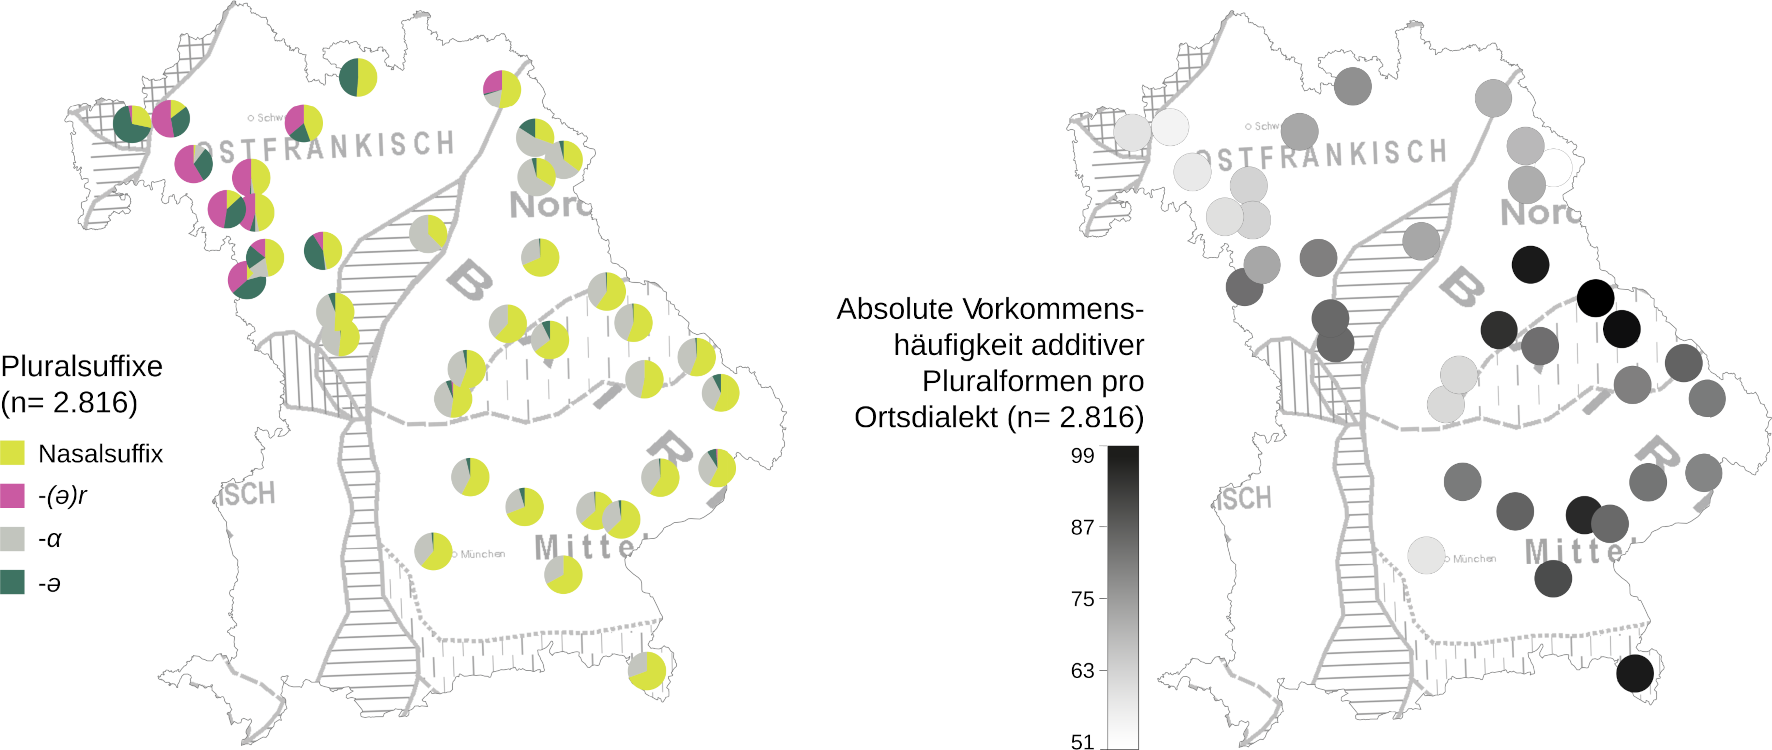
\includegraphics[width=\textwidth]{figures/Karte3.png}
\caption{Häufigkeitsverteilung der Pluralsuffixe und Chloroplethkarte der absoluten Vorkommenshäufigkeit additiver Pluralmarkierung}
\label{map:3}
\end{map}

\mapref{map:3} illustriert, dass additive Pluralmarkierung hinsichtlich der Distribution der einzelnen Pluralsuffixe dialektspezifisch ist (vgl. \sectref{sec:7.1.1.1}). Daneben bestehen areale Unterschiede in der absoluten Vorkommenshäufigkeit additiver Pluralformen, wie die Chloroplethkarte zeigt.

An dieser Stelle ist es sinnvoll, auf Genus als Konditionierungsfaktor von Deklinationsklassen vorzugreifen, da das Raumbild durch den relativen Anteil additiver Pluralmarkierung bei Feminina zu erklären ist (vgl. \sectref{sec:8.3.1.3}). Die Mosaik-Plots\footnote{Sämtliche Mosaik-Plots wurden erstellt mit dem R-Paket \textit{languageR} von Harald Baayen (vgl. \citealt{Baayen2015}, \url{https://www.rdocumentation.org/packages/languageR}).} in \figref{fig:3} visualisieren die Variablen Ortsdialekt (von West nach Ost), Pluralmarkierungstypus\footnote{An dieser Stelle handelt es sich um eine relativ grobe Differenzierung der Pluralmarkierungstypen; zur additiven Markierung werden hier auch kombinierte Verfahren aus Addition und stammaffizierender Markierung, z.\,B. UL+\textit{er}{}-Plural gezählt.}  und absolute Häufigkeit für die drei Genera. Die Flächen der einzelnen Rechtecke sind in ihrer Größe proportional zur Anzahl der Belege, was wiederum einen relativen Vergleich der absoluten Vorkommenshäufigkeit zwischen den Untersuchungsorten ermöglicht (vgl. \citealt[33]{Baayen2015}). Additive Pluralmarkierung
ist demnach ein besonderes frequentes Pluralmarkierungsverfahren für Feminina im südlichen Nordbair. und im Mittelbair., während im restlichen UG Nullplurale den frequenteren Markertypus bilden. Die Extrempunkte bilden das mittelbair.-südbair. Ramsau mit einem Anteil von 77\,\% additiven Pluralen (gegenüber 6\,\% Null und 17\,\% stammaffizierend) und das ofr. Wiesthal mit einem Anteil von 10\,\% an additiven Pluralen (gegenüber 70\,\% Null und 20\,\% stammaffizierend).\footnote{Die absoluten Zahlen sind für Ramsau 78 Belege (60 additiv, 5 Null, 13 stammaffizierend) und für Wiesthal 87 Belege (9 additiv, 61 Null, 17 stammaffizierend).} Auch bei Maskulina und Neutra variiert der relative Anteil von additiven Pluralen im Dialektvergleich, wenn auch weniger deutlich. Bei den Neutra stellt additive Markierung dialektübergreifend das frequenteste Verfahren dar, bei Maskulina hat sie den geringsten Anteil. Wie diese Unterschiede im Einzelnen zu erklären sind und inwiefern sich die konkrete formale Realisierung des additiven Verfahrens bei den Genera unterscheidet, wird im Folgenden und in \chapref{chap:8} mit Blick auf die Zusammensetzung der Deklinationsklassen dargestellt.


\begin{figure}
\begin{subfigure}{\textwidth}\centering
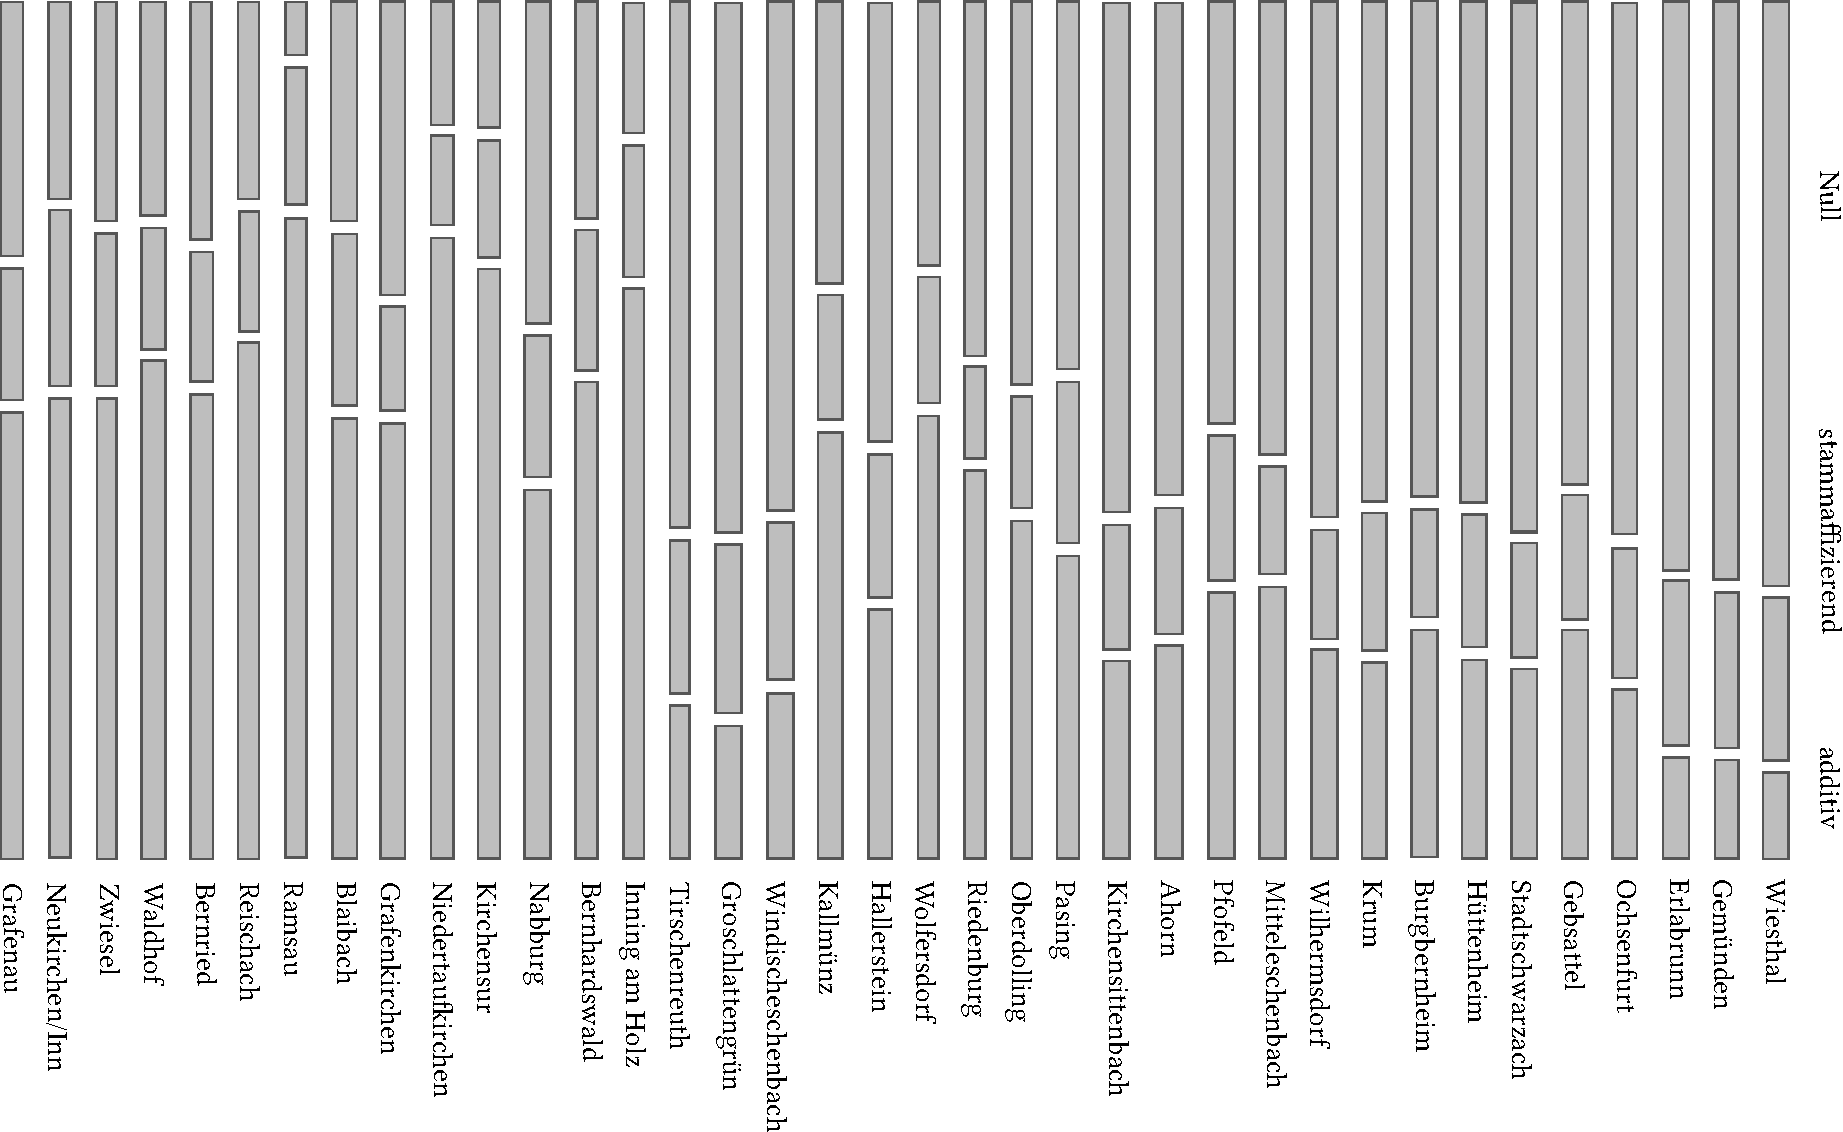
\includegraphics[height=.875\textwidth,angle=90]{figures/revisedNickelNominalmorphologie-img009a.pdf}
\caption{Feminina ($n=3.108$)}
\label{fig:3a}
\end{subfigure}
\caption{Mosaik-Plot der Häufigkeitsverteilung von additiver, stammaffizierender und Nullmarkierung bei den drei Genera (insgesamt $n=7.945$)}
\label{fig:3}
\end{figure}
\begin{figure}\ContinuedFloat
\begin{subfigure}{\textwidth}\centering
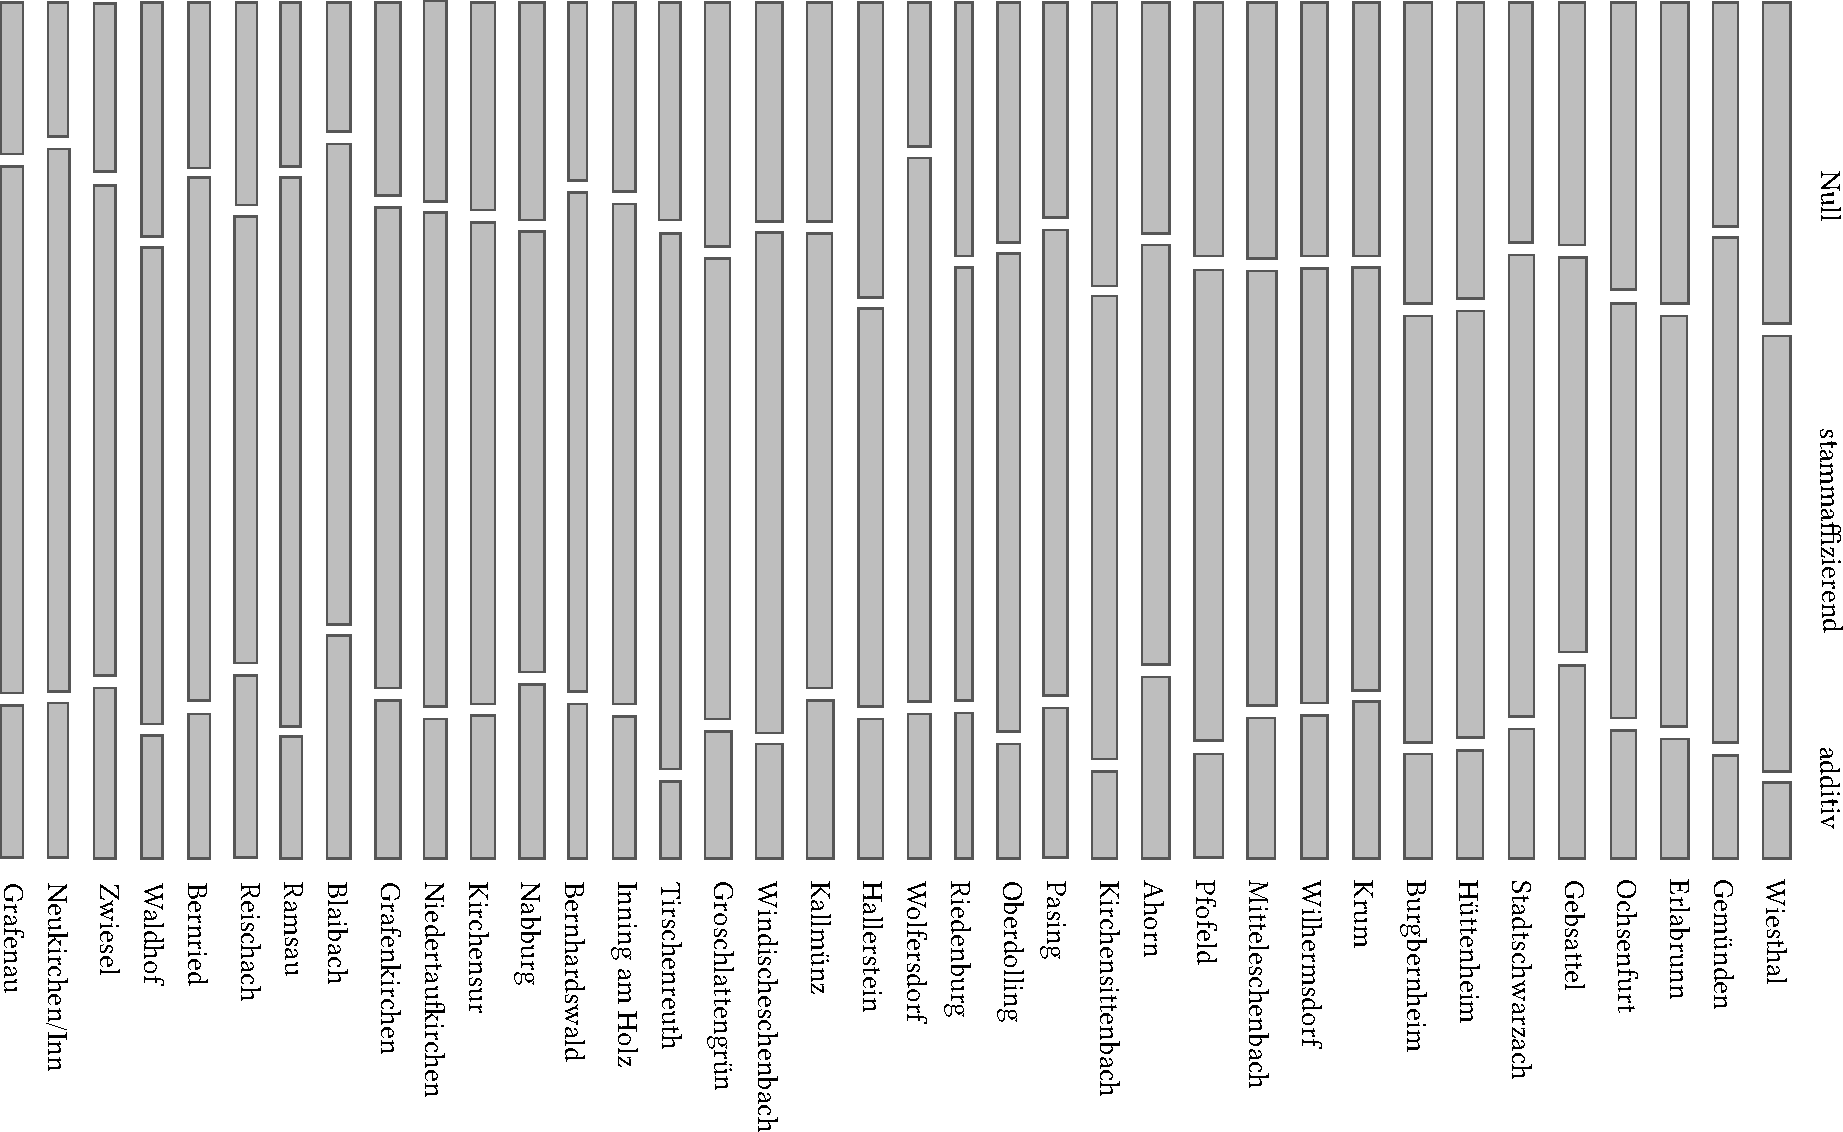
\includegraphics[height=.9\textwidth,angle=90]{figures/revisedNickelNominalmorphologie-img009b.pdf}
\caption{Maskulina ($n=3.426$)}
\label{fig:3b}
\end{subfigure}
\end{figure}
\begin{figure}\ContinuedFloat
\begin{subfigure}{\textwidth}\centering
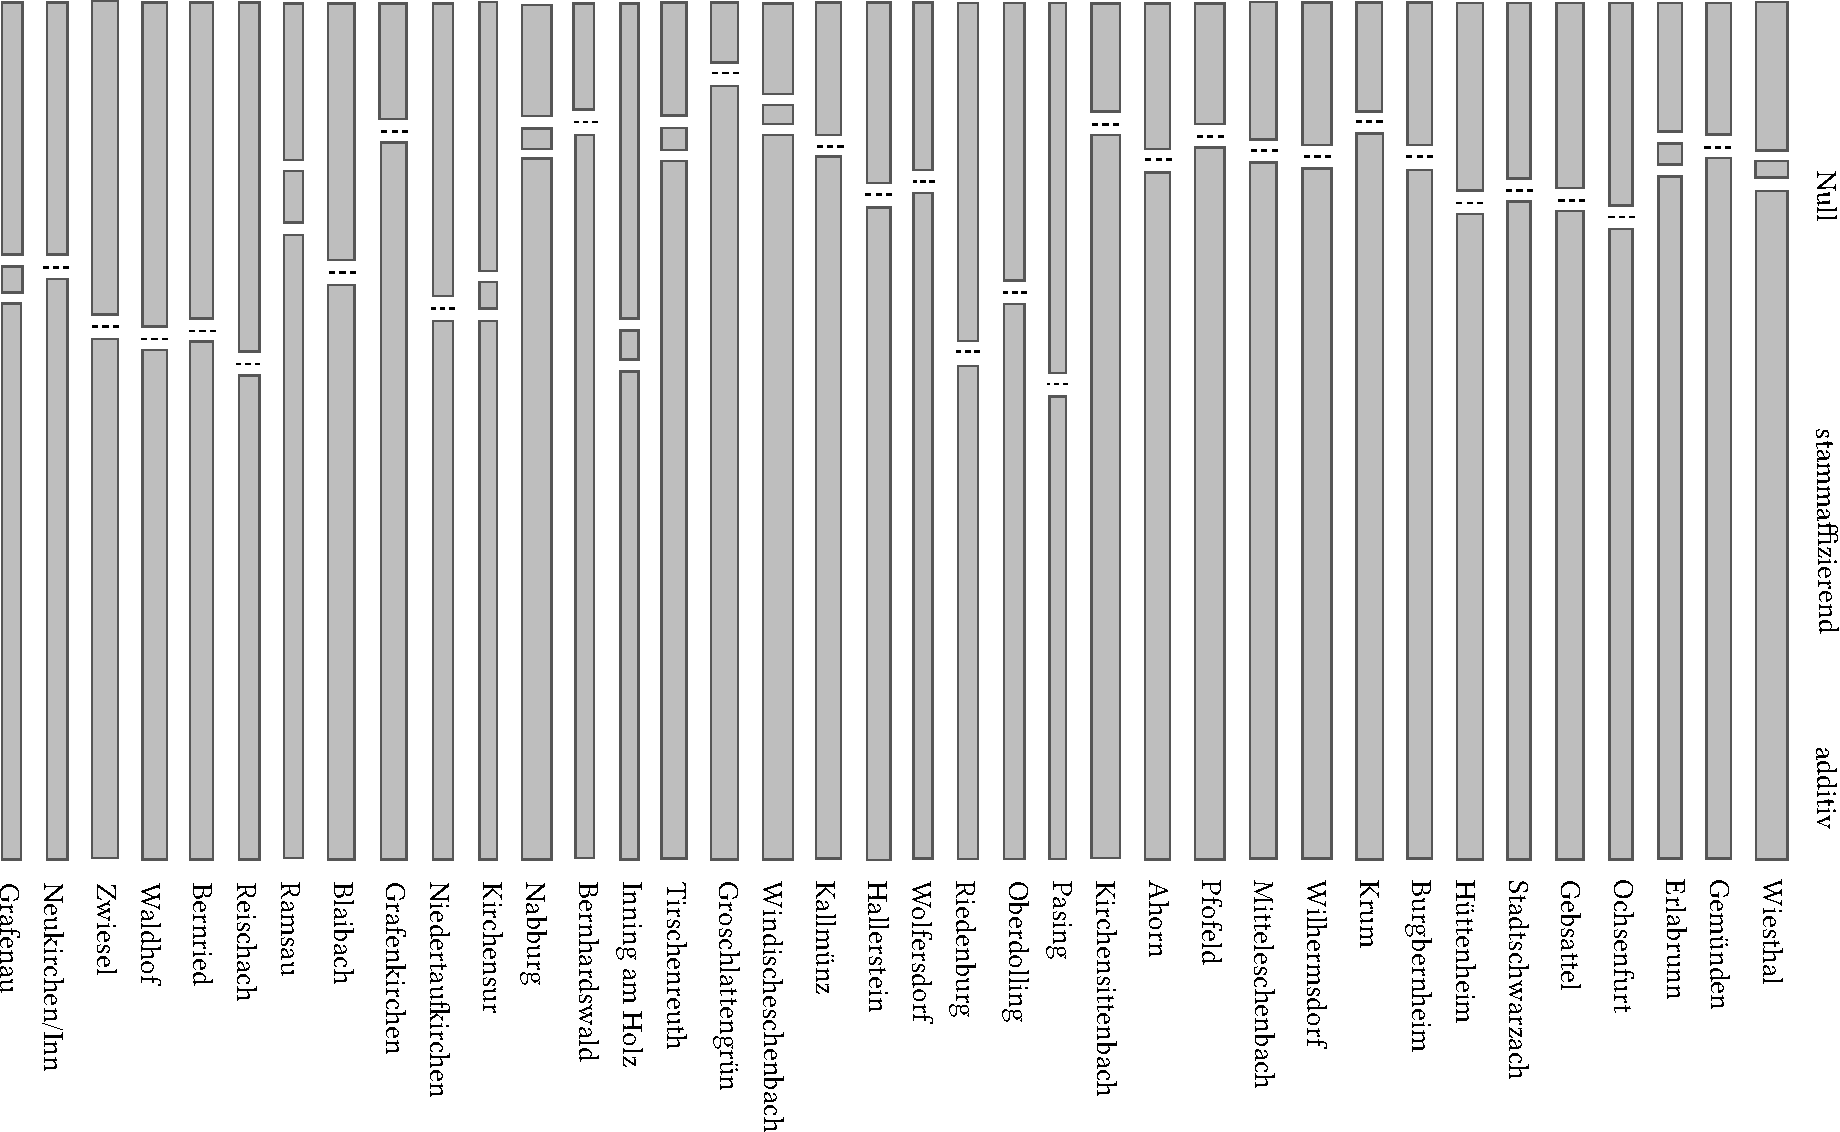
\includegraphics[height=.9\textwidth,angle=90]{figures/revisedNickelNominalmorphologie-img009c.pdf}
\caption{Neutra ($n=1.411$)}
\label{fig:3c}
\end{subfigure}
\end{figure}



\subsubsection{Inventar der Pluralsuffixe}
\label{sec:7.1.1.1}
Additive Pluralmarkierung ist durch Morphophonologie insofern bedingt, als das synchrone Inventar und die areale Verteilung der Flexionssuffixe das Ergebnis historischer phonologischer Prozesse ist (auf Basis der historischen Deklinationsklassenzugehörigkeit). Die phonologischen Prozesse, die im Bereich der Addition relevant sind, betreffen jeweils die Reduktionssilbe. Infolge der Schwa-Apokope entfällt ein additives Verfahren, die Suffigierung mit dem Schwa-Suffix (vgl. standardsprachlich \textit{Hund-e}). Daneben wird die Reduktionssilbe mhd. -\textit{en} in Teilen des UGs mit elidiertem finalen /n/ realisiert, d.\,h. hier besteht Varianz in der formalen Realisierung der Pluralsuffixe -\textit{en} und -\textit{n} (\textit{Ohr-en}, \textit{Hase-n}) in den rezenten Dialekten. Mit Blick auf diese beiden phonologischen Prozesse leiten sich aus einem kontrastiven Vergleich der Flexionssysteme im UG, zwischen dialektalem und standardsprachlichem System oder einer historischen Sprachstufe, zunächst zwei Fragenkomplexe ab:

\begin{itemize}
\item Wie setzt sich das Suffixinventar in Dialekten mit Schwa-Apokope vs. mit Schwa-Erhalt und jenen mit vs. ohne wortfinaler \textit{n}{}-Elision zusammen? Inwiefern variiert (in strukturalistischer Terminologie) der \textit{valeur} der einzelnen Suffixe, d.\,h. ihre Funktionalität und Distribution im jeweiligen Flexionssystem?
\item Lassen sich in apokopierenden Dialekten flexivische Verfahren identifizieren, die Numerussynkretismus infolge der Apokope des Schwa-Suffixes „kompensieren“, und wie sehen diese aus (vgl. \citealt[1197--1198]{Dingeldein1983}, \citealt[135]{Girnth2006}, \citealt[163--164]{Schirmunski1962})?
\end{itemize}

Im oobd. Sprachraum setzt dieApokope in der zweiten Hälfte des 13. Jahrhunderts ein. In Texten des Zeitraums zwischen 1300 und 1350 ist das Pluralsuffix -\textit{e} der alten mask. \textit{a}{}- und \textit{i}{}-Deklination im Bair. und im alem.-bair. Übergangsgebiet bereits zu 100\,\% apokopiert (\citealt[136]{KleinEtAl2018}). Die untersuchten Ortsdialekte des UG gehören zum obd. Apokopegebiet, wenngleich \citet[51 und 203]{Birkenes2014} zeigt, dass es problematisch ist, von rein apokopierenden vs. schwa-erhaltenden Dialekten auszugehen, da es zu wenige empirische Studien über den Status des Schwa in den deutschen Dialekten gibt; vielmehr handele es sich um Tendenzen, da die Apokope einen natürlichen phonologischen Prozess darstelle.

Die Zusammenschau der relevanten Wenker-Karten\footnote{Vgl. die Wenker-Karten zum Nominalbereich mit den Substantivformen des Nom.Pl. (108 „Füße“, 188 „Gänse“, 520 „Leute“, 406 „Berge“), des Dat.Sg. (373/374 „Hause“, 451 „Tische“, 524 „Felde“), die Singularformen mhd. schwacher Feminina (223 „Flasche“, 444 „Seife“, 550 „Wiese“) sowie die schwachen Adjektivformen (43 „gute“, 45 „alte“, 59 „kalte“, 319 „neue“, 531 „brauen“).} zeigt, dass die Untersuchungsorte trotz variierender Isoglossen jeweils im obd. Apokopegebiet liegen. Allerdings finden sich Pluralformen mit Schwa-Suffix für \textit{Gänse} und \textit{Berge} im ofr. Pfofeld (\textit{die bäsen Gänse} ‚die bösen Gänse‘), im ofr. Hallerstein (\textit{Uns’er Berge} ‚unsere Berge‘) und im ofr.-hess. Wiesthal (\textit{onr Berge}). Auf den ersten Blick lässt sich hier nicht sagen, ob es sich um standardnahe Formen handelt oder ob Schwa im dialektalen Suffixinventar auch im obd. Apokopegebiet anzusetzen ist. \mapref{map:3} illustriert, dass additive Formen mit Schwa-Suffix insbesondere im ofr. Teil des UGs durchaus zu finden sind, z.\,B. \teuthoo{hu.nd}{huͅnd} -- \teuthoo{hu.ndE}{huͅndə} ‚Hund‘ (ofr. Gebsattel). Dieses Schwa (und damit die gesamte Pluralform) gleicht in der rezenten Form der standardsprachlichen Form \textit{Hunde}, allerdings unterscheiden sich die Tiefenstrukturen: In der standardsprachlichen Form wird der Plural mit Schwa-Suffix markiert, während die dialektale Form auf die Form *\textit{hund-en} (und damit einen Deklinationsklassenwechsel) zurückgeht, in der das wortfinale /n/ getilgt wurde. Wortfinales Schwa ist in „geschützter Stellung“ \citep[203]{Birkenes2014} vor Nasal damit auch in apokopierenden Dialekten zu finden, vgl. die apokopierte Singularform und die Pluralform mit Schwa-Suffix im ofr. Gemünden am Main: \teuthoo{ho.2s5}{hōͅs̩} -- \teuthoo{ho.2sE}{hōͅsə} ‚Hase‘.

Die Realisierung des Nasalsuffixes mhd. \textit{en} erfolgt in den untersuchten Dialekten in Abhängigkeit von der phonologischen Umgebung. In einem breiten Streifen im Alemannischen und westlichen Ofr. („etwa bis Würzburg“, \citealt[387]{Schirmunski1962}) wird auslautender Nasal in Reduktionssilbe in allen phonologischen Umgebungen elidiert.\footnote{Vgl. \citet[46h]{Kranzmayer1956}, \citet[401]{Rowley1990a}, \citet[143]{Brenner1895} sowie \citet[68--69]{Kemmeter1924}, \citealt[Karte 120]{SBS9.1} und \citealt{WA}-Karte 546 „hinten“ zur Arealität in diesem Teil des Ofr.} Im übrigen Ofr. sowie im Nord- und Mittelbair. ist die Nasaltilgung durch den vorausgehenden Konsonanten bedingt.\footnote{Vgl. \citet[§95.2]{Gebhardt1907}, \citet[Karte 23]{Gütter1971}, \citet[§11]{Frommann1857}, \citet[42]{Hinderling1980}, \citet[Karte 24]{Kranzmayer1956}, \citet[425]{Rowley1990b}, \citet[76--77 und Karte 19]{Rowley1997}, \citet[§582--585]{Schmeller1821}, \citealt{WA}-Karte 444 „Seife“, \citet[101--104]{Wildfeuer2001}.} 	\tabref{tab:16} zeigt anhand exemplarischer Ortsdialekte, dass die vokalische Realisierung von -\textit{en} nach Nasal im gesamten UG erfolgt und gebietsweise nach Stammvokal (Langvokal oder Diphthong),\footnote{Im Datenmaterial ist nur das zweisilbige \textit{Klaue} belegt, das im Ofr. (inklusive ofr.-nordbair. Übergangsgebiet) mit vokalischem Suffix realisiert wird (z.\,B. \teuthoo{gla4<o4u\^A94}{ɡlậọü̯α\klammeruntenpost{}̣} -- \teuthoo{gla4<o4u\^A94}{ɡlậọü̯α\klammeruntenpost{}̣} im ofr. Wilhermsdorf). Im Nord- und Mittelbair. finden sich vor allem nicht-suffigierte Formen im Singular und Plural, daneben vereinzelte Formen mit Nasal (\teuthoo{glôo.<u}{ɡl{\aufstrih}ôͅu} -- \teuthoo{glôo.<un}{ɡl{\aufstrih}ôͅun} im nordbair. Oberdolling) und vokalischem Suffix (\teuthoo{gðlôo4<{gðlôo4<\&ûu.<e4}ûu.<e4}{ɡ̩l{\aufstrih}ộ̃̃{\aufstrih}ûͅẹ} -- \teuthoo{gðlôo4<{gðlôo4<\&ûu.e4n}ûu.e4n}{ɡ̩l{\aufstrih}ộ̃̃{\aufstrih}uͅẹn} im mittelbair. Reischach).} im südlichen Nordbair. und im Mittelbair. zudem nach mhd. \textit{ch}, \textit{f}, \textit{ff}, \textit{pf}, \textit{k}. Nach mhd. \textit{gg} in \textit{Brücke}, \textit{Mücke}, \textit{Glocke}, nach Dental sowie nach den bilabialen Plosiven /p/, /b/ wird -\textit{en} dagegen als Nasal realisiert (ausgenommen ist hier der Vokalisierungsstreifen im westlichen Ofr.).


\begin{table}
\small
\begin{tabularx}{\textwidth}{QQQQQQ}
\lsptoprule
& {Tanne}

 (mhd. \textit{n}) & {Seife}

 (mhd. \textit{f}) & {Eiche}

 (mhd. \textit{(c)h}) & {Stecken}

 (mhd. \textit{k}) & {Karpfen/}

{ Schupfen}

 (mhd. \textit{pf})\\
 \midrule
westl. Ofr.

(Erlabrunn) & \teuthoo{da.nA}{daͅnα} -- \teuthoo{da.nA}{daͅnα} & Sg. \teuthoo{se.v5A94}{seͅv̩α\klammeruntenpost{}̣} & \teuthoo{e.cE}{eͅXə} -- \teuthoo{e.cE}{eͅXə} & Sg. \teuthoo{A4n}{α̣n} \teuthoo{s\#da4gA)4}{šdạɡα\klammeruntenpost{}̣} & {\teuthoo{kharbv5E}{kharbv̩ə} --}

 \teuthoo{kharbv5E}{kharbv̩ə}

\teuthoo{s\#u.bE}{šuͅbə} -- \teuthoo{s\#u.bE}{šuͅbə}\\
\tablevspace
Ofr.

(Wilherms\-dorf) & \teuthoo{da.nA94}{daͅnα\klammeruntenpost{}̣} -- \teuthoo{da.nA94}{daͅnα\klammeruntenpost{}̣} & \teuthoo{sa42v5m}{sạ̄v̩m} -- \teuthoo{sa42v5m}{sạ̄v̩m} & \teuthoo{a94xY}{a\klammeruntenpost{}̣x{\klammerNG}} -- \teuthoo{a94xY}{a\klammeruntenpost{}̣x{\klammerNG}} & \teuthoo{s\#de9.gY}{šde\klammeruntenpost{}ͅɡ{\klammerNG}} -- \teuthoo{s\#de9.gY}{šde\klammeruntenpost{}ͅɡ{\klammerNG}} & {\teuthoo{k\_a.rbv5m}{kʰaͅrbv̩m} --}

 \teuthoo{k\_a.rbv5m}{kʰaͅrbv̩m}\\
 \tablevspace
nördl. Nordbair.

(Grosch\-latten\-grün) & \teuthoo{d5å"nA}{d̩{\burgeroalphamakron}nα} -- \teuthoo{d5å"nA}{d̩{\burgeroalphamakron}nα} & \teuthoo{so9.i.fm@}{so\klammeruntenpost{}ͅiͅfm̥} -- \teuthoo{so9.i.fm@}{so\klammeruntenpost{}ͅiͅfm̥} & \teuthoo{qo.<i.cN@}{ʔôͅiͅXŋ̥} -- \teuthoo{qo.<i.cN@}{ʔôͅiͅXŋ̥} & \teuthoo{s\#de.kqN@}{šdeͅkʔŋ̥} -- \teuthoo{s\#de.kqN@}{šdeͅkʔŋ̥} & {\teuthoo{g\_o3Apfm@}{ɡʰŏαpfm̥} --}

 \teuthoo{g\_o3Apfm@}{ɡʰŏαpfm̥}

\teuthoo{s\#upfm@}{šupfm̥} -- \teuthoo{s\#upfm@}{šupfm̥}\\
\tablevspace
südl. Nordbair./

nordbair.-mittelbair. Übergangs\-gebiet

(Kallmünz) & \teuthoo{da.nA}{daͅnα} -- \teuthoo{da.nAn}{daͅnαn} & \teuthoo{so.ifA}{soͅifα} -- \teuthoo{so.ifAn}{soͅifαn} & \teuthoo{o.iX!A}{oͅiꭖα}-- \teuthoo{o.ic1An}{oͅiX\⚬αn} & {\teuthoo{s\#de.kA}{šdeͅkα} --}

 \teuthoo{s\#de.kAn}{šdeͅkαn} & {\teuthoo{k,\_a.rpfA}{k͓ʰaͅrpfα} --}

 \teuthoo{k\_arpfAn}{kʰarpfαn}

\teuthoo{s\#u.pfA}{šuͅpfα}-- \teuthoo{s\#u.pfAn}{šuͅpfαn}\\
\tablevspace
Mittelbair.

(Grafenau) & {\teuthoo{A}{α} \teuthoo{d5e."+nA}{d̩ẽ̄ͅnα} --}

 \teuthoo{de.>+nAn}{dễͅnαn}, \teuthoo{de.>+nAne4}{dễͅnαnẹ} & {\teuthoo{s5o.<Af,E}{s̩ôͅαf͓ə} --}

 \teuthoo{s\%o.<AfEn}{s͈ôͅαfən} & {\teuthoo{o9.<AxA}{o\klammeruntenpost{}̂ͅαxα} --}

 \teuthoo{o9.<AxAn}{o\klammeruntenpost{}̂ͅαxαn} & Sg. \teuthoo{s\#5d5ekA}{š̩d̩ekα} & {\teuthoo{s\#u.b\%v\%A}{šuͅb͈v͈α} --}

 \teuthoo{d5s\#5u.pfAn}{d̩š̩uͅpfαn}\\
 \tablevspace
mittelbair-südbair. Übergangsgebiet (Ramsau) & \teuthoo{d\%a.<n}{d͈âͅn} -- \teuthoo{d\%a.nA}{d͈aͅnα} & \teuthoo{s\%oAfð5}{s͈oαf̩̩} -- \teuthoo{s\%oa4fn@}{s͈oạfn̥} & \teuthoo{o4a4X!}{ọạꭖ} -- \teuthoo{o4a4X!Y@}{ọạꭖ{\klammerNG}̥} & Sg. \teuthoo{s\#\%t,e.kHEY}{š͈t͓eͅkhͯə{\klammerNG}} & {}--\\
\lspbottomrule
\end{tabularx}
\caption{Realisierung der Reduktionssilbe -\textit{en} in standardsprachlichen Zweisilbern in der Singular- und Pluralform (sofern in den Daten belegt) in exemplarischen Ortspunkten des UG (vgl. Karte 19 in \citealt{Rowley1997})}
\label{tab:16}
\end{table}

An den verschiedenen Formen in 	\tabref{tab:16} fällt auf, dass die Qualität des reduzierten Vokals im UG und auch in den Ortsdialekten variiert (vgl. \citealt[387]{Schirmunski1962}). Die areale Verteilung der vokalischen Pluralsuffixe in \mapref{map:3} illustriert, dass in den ofr. Ortsdialekten vor allem -\textit{\teuthoo{E}{ə}} und -\textit{\teuthoo{E.}{əͅ}} (für den Reduktionsvokal zwischen [\teuthoo{A}{α}] und [\teuthoo{E}{ə}]) belegt ist, während im bair. Teil des UGs (inklusive ofr.-nordbair. Übergangsgebiet) vor allem -\textit{\teuthoo{A}{α}} („Tiefschwa“) und in geringerem Maße -\textit{\teuthoo{E}{ə}} erscheint (vgl. \citealt[6]{Mausser1915}).\footnote{Daneben findet sich in den bair. Ortsdialekten teilweise Vollvokal (vgl. \teuthoo{mo.<Ak}{môͅαk} -- \teuthoo{me.<k,t,e4}{mêͅk͓t͓ẹ} ‚Markt‘ im mittelbair. Reischach und \teuthoo{s\#ta42l}{štạ̄l} -- \teuthoo{s\#ta4<l"e4}{štậl̄ẹ} ‚Starl‘ im mittelbair. Wolfersdorf mit vorderem [\teuthoo{e.}{eͅ}] und \teuthoo{nuS}{nuʃ} -- \teuthoo{ni.ʃ{\textasciitilde}ôe.}{niʃ{\aufstrih}e} ‚Nuss‘ im nordbair. Groschlattengrün mit zentralisiertem [\teuthoo{e.}{eͅ}]).}  Die Durchsicht der Belege zeigt, dass die Distribution der vokalischen Suffixe in jenen Orten, die verschiedene Abstufungen des Reduktionsvokals oder vereinzelt Vollvokal aufweisen, durch phonetische Variation bedingt ist: Schwa und Tiefschwa erscheinen in den gleichen Kontexten (vgl. \citealt[15]{Köhler1934}). Es ist hier also sinnvoll, phonetische Varianz auf einem Kontinuum zwischen \textit{e}{}- und \textit{a}{}-Färbung anzunehmen, zumal das ausdifferenzierte Notationssystem der Teuthonista diese Abstufungen wiedergibt und hier auch Transkriptionseffekte zu beobachten sind.\footnote{Beispielsweise im ofr. Gebsattel, wo die Singular- und Pluralform von ‚Ratte‘ mit differenter Reduktionssilbe transkribiert ist (\teuthoo{ra94dE.}{ra\klammeruntenpost{}̣dəͅ} -- \teuthoo{ra94dA}{ra\klammeruntenpost{}̣dα}), die Gewährsperson aber angemerkt hat „Sg. + Pl. klingt gleich“.}

Dennoch erscheint es -- zumindest im Rahmen einer ersten Klassifikation -- nicht praktikabel, Schwa und Tiefschwa zu einem einzigen vokalischen Suffix zusammenzufassen. Zum einen gibt es Hinweise in der Literatur, dass -\textit{α} und -\textit{ə} im Ofr. phonologisch distinkt sind (vgl. \citealt[82]{Rowley1997}). So findet sich laut \citet[214--215]{Diegritz1971} im Osten Mittelfrankens eine Opposition zwischen /ɐ/ als synchroner Entsprechung von mhd.-\textit{e}/-\textit{en} und /ə/ für mhd. -\textit{er}/-\textit{ære}, während im westlichen Mittelfranken die Opposition zwischen /ə/ (mhd. -\textit{en}, -\textit{em}, -\textit{e}) und /r/ (mhd. -\textit{er}, {}-\textit{ære}) besteht. In dieser Eindeutigkeit können die Verhältnisse für die ofr. Daten allerdings nicht bestätigt werden. Anderseits gibt es Dialekte -- und hier lohnt ein Blick jenseits des eigenen UGs in das Schwäb. und das mittelbair.-schwäb. Übergangsgebiet --, in denen -\textit{α} und -\textit{ə} tatsächlich phonologisch distinkt sind. In einem kleinen Areal im südlichen SBS-Arbeitsgebiet alterniert das Stammsuffix der mhd. schwachen Feminina zwischen -\textit{ə} im Singular und -\textit{α} im Plural: \teuthoo{A}{α} \teuthoo{nu.<iE@}{nûͅiə̥} \teuthoo{glo4kE}{ɡlọkə} -- \teuthoo{nu.<iE@}{nûͅiə̥} \teuthoo{glo4ka}{ɡlọka} ‚eine neue Glocke/neue Glocken‘ (schwäb. Bernbeuren, vgl. \mapref{map:33}, \sectref{sec:7.1.1.4} sowie \citealt[Karten 105--117]{SBS9.1}, \citealt[8]{Rowley1994}).

\begin{sloppypar}
Für das gesamte Untersuchungsgebiet können folgende Suffixtypen unterschieden werden, das (orts-)dialektspezifische Inventar und die areale Variation der Suffixe ergeben sich jeweils aus dem phonologischen System respektive aus den historischen phonologischen Prozessen:\footnote{Daneben findet sich ein einzelner Beleg für \textit{s}{}-Suffix: Die Gewährsperson in Krum bildet die Pluralform zu ‚Kummet‘ spontan als \teuthoo{khumEds}{khuməds} und bietet anschließend die Form \teuthoo{khumEdn}{khumədn} mit dem Kommentar „besser“. Das \textit{s}-Suffix wird im Folgenden daher nicht weiter berücksichtigt (vgl. \sectref{sec:4.2.1} und \citealt[1199]{Dingeldein1983} zum \textit{s}-Suffix in den deutschen Dialekten).} 
\end{sloppypar}

\begin{itemize}
\item \textit{Nasalsuffix} in den phonetischen Realisierungen [m], [n], [ŋ]: Nach (bi-)""labialem Plosiv oder Frikativ wird das Nasalsuffix zu [m] assimiliert, nach velarem Plosiv zu [ŋ] (vgl. \citealt[Karte 24]{Kranzmayer1956}, \citealt[126 und Karte 220]{Rowley1997}, \citealt[388]{Schirmunski1962}, \citealt[§578--580]{Schmeller1821}).\footnote{Vgl. \citet[57--58]{Kufner1961}, \citet[121]{Steininger1994} zum Mittelbair. sowie \citet[§45.I]{Hain1936}, \citet[67--68]{Kemmeter1924}, \citet[15]{Köhler1934} zum Ofr.} Daneben erfolgt gebietsweise Elision des stammauslautenden Konsonanten \textit{b} (\textit{w}), \textit{d}/\textit{t}, \textit{g}, \textit{r} und \textit{x} vor Nasalsuffix, z.\,B. \teuthoo{gða.rb}{ɡ̩aͅrb} -- \teuthoo{gða.rm}{ɡ̩aͅrm} ‚Garbe‘ (mittelbair. Kirchensur), \teuthoo{saux}{saux} -- \teuthoo{tauN}{tauŋ} ‚Auge‘ (nordbair. Nabburg, vgl. \citealt{Rowley1997}: 126).

Im bair. Teil des UGs wird Nasalsuffix teilweise als Reduktionssilbe mit Tiefschwa [αn] realisiert, vgl. \teuthoo{bre4m}{brẹm} -- \teuthoo{bre4"(+mAn}{brẹ̃̄\klammerobenpost{}mαn} ‚Bremse‘ (mittelbair. Niedertaufkirchen), \teuthoo{le.Ax5}{leͅαx̩} -- \teuthoo{le.<AhA4n}{lêͅαhα̣n} ‚Lärche‘ (mittelbair. Waldhof). Diese Realisierungsform findet sich nur bei historisch zweisilbigen Feminina mit apokopierter Singularform. \citet[§26]{Micko-Repp1933} zufolge handelt es sich um eine Neubildung: An das Suffix -\textit{α}, das lautgesetzlich nach Nasal oder Velarplosiv/-frikativ im Stammauslaut erscheint, wird das Nasalsuffix -\textit{n} gehängt, sodass hier eine Art Doppelsuffigierung entsteht (vgl. \citealt[§49]{Kollmer1985}, \citealt[153]{Rowley1997}). Die Outputstruktur der Pluralform entspricht in der Folge den Pluralformen mit Nasalsuffix der \textit{n}{}-erweiterten Feminina mit vokalisch realisierter Reduktionssilbe: \teuthoo{bre42mA}{brẹ̄mα} -- \teuthoo{bre42mAn}{brẹ̄mαn} ‚Bremse‘ (mittelbair. Pasing), \teuthoo{le.AXA}{leͅαꭗα} -- \teuthoo{le.AXAn}{leͅαꭗαn} ‚Lärche‘ (nordbair.-mittelbair. Zwiesel, siehe hierzu ausführlicher Abschnitte~\ref{sec:7.1.1.3} und \ref{sec:8.3.3.1})

\item \textit{\textit{(ə)r}{}-Suffix}
\item \textit{\textit{α}}\textit{{}-Suffix} als vokalische Realisierung von mhd. -\textit{er}, mhd. -\textit{en}
\item \textit{\textit{ə}}\textit{{}-Suffix} als vokalische Realisierung von mhd. -\textit{er}, mhd. -\textit{en}
\end{itemize}

Die oben beobachtete Zweiteilung des UGs in ein bair. vs. ofr. Gebiet setzt sich in der arealen Distribution der Suffixe und in der ortsdialektspezifischen Zusammensetzung des Suffixinventars fort. Im bair. Teil (inklusive nordbair.-ofr. Übergangsgebiet) findet sich ein -- im historischen wie interdialektalen Vergleich -- reduziertes Inventar mit Nasal- und \textit{α}{}-Suffix (daneben teilweise Schwa-Suffix). Neben dem Pluralsuffix mhd. -\textit{en} in bestimmten phonologischen Umgebungen wird auch die Reduktionssilbe mhd. -\textit{er} im bair. Teil des UG vokalisiert als -\textit{α} realisiert, weshalb das \textit{α}{}-Suffix in diesen Dialekten (mit Bezug auf das standardsprachliche System oder eine historische Sprachstufe) „tiefenstrukturell mehrdeutig“ \citep[127]{Rowley1997} ist.\footnote{Vgl. \citet[113]{Haas1983}, \citet[§50c3 und Karte 26]{Kranzmayer1956}, \citet[65]{RennKönig2006}, \citet[82 und Karte 19]{Rowley1997}, \citet[257 und Karte 9]{Werner1961} sowie die \citealt{WA}-Karten 4 „Winter“, 61 „Wasser“, 105 „Pfeffer“.} Das Suffixsystem dieses Typs unterscheidet sich von Systemen, in denen mhd. -\textit{er} und mhd. -\textit{en} auch synchron unterschieden sind, etwa in einem Teil des Unterofr., wo die Reduktionssilbe mhd. -\textit{er} als konsonantisches [r] und mhd. -\textit{en} vokalisch realisiert wird. In den übrigen ofr. Tiefenbohrungspunkten besteht Variation in der spezifischen Verteilung konsonantischer und vokalischer Pluralsuffixe in Abhängigkeit von den phonologischen Systemen. Im ofr. Stadtschwarzach und Hüttenheim beispielsweise werden mhd. -\textit{er} und -\textit{en} konsonantisch realisiert, nur nach Nasal und Stammvokal erfolgt Elision des wortfinalen /n/, sodass die Distribution von Nasal- und (Tief-)Schwa-Suffix hier phonotaktisch konditioniert ist (vgl. \sectref{sec:8.3.3.2}). In den übrigen Orten erscheinen sowohl vokalische als auch konsonantische Realisierung von mhd. -\textit{er} und -\textit{en}. Schwa und Tiefschwa sind auch hier „tiefenstrukturell mehrdeutig“, da sie vokalische Realisierungen von mhd. -\textit{er} und -\textit{en} repräsentieren.

Die methodische Schwierigkeit der Analyse besteht nun darin, die Distribution der vokalischen Suffixe auf der phonetischen und auf der morphophonologischen Ebene adäquat abzubilden (vgl. \citealt[40--43]{Hinderling1980}, \citealt[126--129]{Rowley1997}, \citealt[29--30]{SMF7}). Eine Möglichkeit der Analyse besteht darin, die jeweiligen konsonantischen und vokalischen Realisierungen als eigene Suffixtypen zu klassifizieren und damit v.\,a. die synchrone Perspektive zu berücksichtigen (vgl. z.\,B. \citealt[38]{Gladiator1971} und \citealt[57--60]{Kufner1961}). Demnach würden die Suffixe der Flexionsformen von \textit{Hase} im westlichen Ofr. der phonetischen Realisierung entsprechend als drei verschiedene Flexionssuffixe -\textit{ən}, -\textit{ə}, -\textit{α} klassifiziert, vgl. Nom.Sg. \teuthoo{ho9.2s5}{ho\klammeruntenpost{}̄ͅs̩} -- Akk.Sg. \teuthoo{ho9.2sn@}{ho\klammeruntenpost{}̄ͅsn̥} -- Nom.Pl. \teuthoo{ho9.2sn@}{ho\klammeruntenpost{}̄ͅsn̥} (ofr. Burgbernheim), \teuthoo{ho.2s5}{hōͅs̩} -- \teuthoo{ho.2sE}{hōͅsə} --\teuthoo{ho.2sE}{hōͅsə} (ofr. Gebsattel), \teuthoo{ha.2s5}{hāͅs̩} -- \teuthoo{An}{αn} \teuthoo{ha2.sA}{hāͅsα} -- \teuthoo{ha:2sA}{ha{\doubleogonek}̄sα} (ofr. Erlabrunn).\footnote{\citet[38]{Gladiator1971} analysiert das \textit{α}{}-Suffix als Allophon des Phonems /a/ gegenüber den Suffixen [m, n, ŋ] als Allophon von /-n/, da /a/ und /-n/ im Wortauslaut in Opposition stehen könnten, z.\,B. /hɔasa/ ‚heißer‘ vs. /hɔasn/ ‚heißen‘. In dieser Lösung wird die „tiefenstrukturelle“ Mehrdeutigkeit \citep[127]{Rowley1997} der Flexive -\textit{er} und -\textit{en} nicht aufgelöst, \textit{α}{}- und Nasalsuffix werden rein synchron klassifiziert. Anders geht \citet[§27]{Micko-Repp1933} vor, die das \textit{α}{}-Suffix auf -\textit{er} zurückführt, das von den Neutra auf Feminina und Maskulina übertragen wurde.}

Eine alternative Form der Analyse besteht in der Klassifikation von -\textit{ən}, -\textit{ə}, \mbox{-\textit{α}} als Heteromorphe des Nasalsuffixes, deren Distribution durch phonologische Faktoren dialektspezifisch gesteuert ist. Diese Form der Klassifikation ist hier naheliegend, da sich aus Obliquus- und Pluralform die Zuweisung zur schwachen Deklination ergibt. Eine eindeutige Klassifikation von Schwa und Tiefschwa als rezenter Entsprechung des Nasal- oder \textit{er}{}-Suffixes ist allerdings nicht in allen Fällen möglich, wie beispielsweise Pluralformen des Typs \teuthoo{ba2mA}{bāmα} ‚Baum‘ im Nordbair. zeigen (vgl. \citealt[128]{Rowley1997}). Mhd. -\textit{er} und mhd. -\textit{en} in der phonologischen Umgebung nach Nasal werden in diesem Gebiet jeweils als [α] realisiert. Daneben ist im Übergangsgebiet von zentralem und westlichem SMF-Untersuchungsgebiet Tiefschwa als Pluralmarker von \textit{Fleck} nicht eindeutig als Entsprechung von -\textit{er} oder -\textit{en} zu klassifizieren, da in diesem Areal beide Formen belegt sind (\citealt[29--30]{SMF7}). Zudem bleibt bei der zweiten Lösungsvariante offen, inwiefern -\textit{α} als rezente Entsprechung von -\textit{er} und -\textit{en} oder tatsächlich als eigenständiges Pluralsuffix mental repräsentiert ist. \citet[129]{Kalau1984} berichtet beispielsweise von der Verwechselung der standardsprachlichen Pluralsuffixe -\textit{er} und -\textit{en} bei Sprechern des Nürnberger Dialekts, wo beide Suffixe als -\textit{α} realisiert werden. Da es Ziel der synchronen Analyse ist, die Faktoren der Distribution der einzelnen Suffixe auf der Ebene des Einzeldialekts zu erarbeiten, wird auf eine abstrahierende Klassifikation zunächst verzichtet. Die Annotation der Suffixe erfolgte daher entsprechend ihrer phonetischen Realisierung.

\subsubsection{Kombinierte Verfahren}
\label{sec:7.1.1.2}
Neben rein additiven Pluralformen tritt das Pluralsuffix in Kombination mit einem oder mehreren stammaffizierenden Pluralmarkierungsverfahren auf (\tabref{tab:17}).


\begin{table}
\begin{tabularx}{\textwidth}{>{\raggedright\arraybackslash}p{.2\textwidth}lQ}
\lsptoprule

\multicolumn{3}{l}{Kombiniertes Verfahren aus Addition und \ldots}\\
\midrule
\multirow[t]{2}{=}{Kontrasten der Vokalqualität} & Umlaut & \teuthoo{s\#du.2m}{šdūͅm} -- \teuthoo{ds\#di“mA}{dšdīmα} ‚Stube‘ (nordbair.-mittelbair. Bernhardswald)\\
& mhd. \textit{ei} & \teuthoo{o2A}{ōα} -- \teuthoo{qo.<i.A}{ʔôͅiͅα} ‚Ei‘ (nordbair. Groschlattengrün)\\
\tablevspace
\multicolumn{2}{p{.4\textwidth}}{Kontrasten der Vokalquantität} & \teuthoo{no2l}{nōl} -- \teuthoo{noln}{noln} ‚Nadel‘ (mittelbair. Grafenau)\\
\tablevspace
\multicolumn{2}{>{\raggedright\arraybackslash}p{.4\textwidth}}{Umlaut + Kontrasten der Vokalquantität} & \teuthoo{ro42d}{rọ̄d} -- \teuthoo{re.3dA}{rĕͅdα} ‚Rad‘ (ofr. Pfofeld)\\
\tablevspace
\multirow[t]{2}{=}{Konsonantismus\-kontrasten} & Elision & \teuthoo{v5i“}{v̩ī} -- \teuthoo{v5i“cE}{v̩īXə} ‚Vieh‘ (ofr. Krum)\\
& \makecell[tl]{Lenis-Fortis-\\Kontraste} & \teuthoo{ho.ds}{hoͅds} -- \teuthoo{hôoi4tSA}{h{\aufstrih}oịtʃα} ‚Holz‘ (nordbair.-mittelbair. Blaibach)\\
\tablevspace
\multicolumn{2}{p{.4\textwidth}}{Lenis-Fortis-Kontrasten + Quantitätskontrasten} & \teuthoo{ne42sd}{nẹ̄sd} -- \teuthoo{ne4StA}{nẹʃtα} ‚Nest‘ (nordbair.-mittelbair. Zwiesel)\\
\tablevspace
\multicolumn{2}{p{.4\textwidth}}{Lenis-Fortis-Kontrasten + Quantitätskontrasten + Umlaut} & \teuthoo{vo2s}{vōs} -- \teuthoo{va4SA}{vạʃα} ‚Fass‘ (nordbair. Nabburg)\\
\lspbottomrule
\end{tabularx}
\caption{Übersicht kombinierter Pluralmarkierungsstrategien}
\label{tab:17}
\end{table}

Die einzelnen stammaffizierenden Verfahren werden in \sectref{sec:7.1.2}, deklinationsklassenspezifische Faktoren der Distribution in \sectref{sec:8.3} dargestellt.

\subsubsection{„Doppelsuffigierung“: -\textit{α} und -\textit{αn} im Bair.}
\label{sec:7.1.1.3}
Eine dialektraumspezifische Form additiver Pluralmarkierung findet sich im bair. Teil des UGs bei historisch zweisilbigen Feminina mit Schwa-Reduktionssilbe, die in der Singularform Nasalsuffix aufweisen (Typ \textit{Glocke-n}), das in Abhängigkeit von der phonologischen Umgebung des vorausgehenden Lauts als -\textit{n} oder vokalisch als -\textit{α} realisiert wird (vgl. \sectref{sec:7.1.1.1} und 	\tabref{tab:16}). Je nach konsonantischer oder vokalischer Realisierung der Reduktionssilbe erfolgt die additive Pluralmarkierung durch Nasal- oder Tiefschwa-Suffix, z.\,B. \teuthoo{biEkA}{biəkα} -- \teuthoo{biEkAn}{biəkαn} ‚Birke‘ (nordbair. Nabburg), \teuthoo{glok-N}{ɡlok{}͐ŋ} -- \teuthoo{glok-nA}{ɡlok{}͐nα} ‚Glocke‘ (mittelbair. Grafenau), sodass eine Art Doppelsuffigierung aus Stammbildungssuffix\footnote{Da es im Dialektvergleich und lexemweise auch im Ortsdialekt Variation zwischen Singularformen mit apokopierter Schwa-Reduktionssilbe und \textit{n}{}-Erweiterung gibt (z.\,B. \teuthoo{s\#dro2S}{šdrōʃ} neben \teuthoo{s\#dro2Sn}{šdrōʃn} ‚Straße‘, eingehender zur Problematik siehe Abschnitte~\ref{sec:7.1.3.1} und \ref{sec:8.2.3}), wird im Folgenden tatsächlich von einem Stammbildungssuffix ausgegangen. Allerdings ist nicht auszuschließen, dass nicht zumindest lexemweise eine Verschiebung der Morphemgrenze stattgefunden hat und die Reduktionssilbe als Teil des Stammes analysiert und abgespeichert wird. Dies scheint insbesondere dann plausibel, wenn eine Assimilation von Stammauslaut und Nasalsuffix vorliegt, etwa in \teuthoo{s\#tum}{štum} ‚Stube‘. Durch die dialektvergleichende Ausrichtung der Untersuchung und das Nebeneinander von apokopierten und \textit{n}{}-erweiterten Formen scheint das Konzept des Stammbildungssuffixes hier aber praktikabler.} der Singularform und Pluralsuffix -\textit{n} bzw. -\textit{α} entsteht, vereinzelt finden sich in den Daten „Trippelsuffigierungen“: \teuthoo{A}{α} \teuthoo{d5e."+nA}{d̩ẽ̄ͅnα} -- \teuthoo{de.>+nAne4}{dễͅnαnẹ} ‚Tanne‘ (mittelbair. Grafenau), \teuthoo{wo42xA}{wọ̄xα} -- \teuthoo{wo42xAnA}{wọ̄xαnα} ‚Woche‘ (nordbair.-mittelbair. Blaibach). Doppelsuffigierungen sind indes kein Spezifikum des Bair. als solches; \citet[838]{Tiersma1982} etwa bietet Beispiele aus dem Niederländischen, wo historische Pluralformen als Singularformen reanalysiert und in der Folge durch einen „double plural“ markiert wurden (mittelniederländisch Sg. \textit{schoe} ‚Schuh‘ > \textit{schoen} -- \textit{schoenen}).

Varianz besteht bezüglich der Form des Pluralsuffixes, es finden sich bei Nasal-Reduktionssilbe vor allem Abfolgen aus Nasal+\textit{α}, vereinzelt aber auch aus Nasal+\textit{αn}, z.\,B. \teuthoo{s\#du.m}{šduͅm} -- \teuthoo{s\#du.mAn}{šduͅmαn} ‚Stube‘ im mittelbair. Niedertaufkirchen. Terminologisch werden diese Doppelsuffigierungen auch als „potenzierter Plural“ gefasst (etwa bei \citealt[431]{Schirmunski1962} oder \citealt[192]{Zehetner1978}). In Dialektgrammatiken werden die Pluralformen aus Stammbildungssuffix und -\textit{n} bzw. -\textit{α} teilweise auch als standardsprachliche Protoform *-\textit{enen} modelliert (vgl. \citealt[§863]{Schmeller1821}, \citealt[187]{Wildfeuer2001}, \citealt[117]{Zehetner1985}). \citet{Mauser1998a, Mauser1998b} analysiert diesen Markierungstypus als Restitution des mhd. Nasalsuffixes, die infolge der Ausweitung des Flexivs der obliquen Kasus auf den Nom.Sg. im Paradigma der historisch schwachen Feminina erfolgte.

\begin{sloppypar}
Die Chloroplethkarten in \mapref{map:4} zeigen, dass additive Pluralmarkierung nach beiden Realisierungsvarianten des Nasalsuffixes im südlichen Nordbair. und im Mittelbair. zu finden ist.\footnote{Vgl. auch die Kombinationskarten des SBS, die zeigen, dass Suffigierungen des Typs -\textit{nα}/-\textit{nə} bei Feminina an der Ostgrenze des SBS-Arbeitsgebiets, d.\,h. im mittelbair.-schwäb. Übergangsgebiet und am Westrand des Mittelbair., besonders frequent sind (\citealt[Karte 117, 122, 131]{SBS9.1}), sowie die SMF-Kombinationskarte mit maximaler Verbreitung sogenannter „potenzierter“ Plurale im Südosten des SMF-Gebiets (\citealt[Karte 1]{SMF7}).} Nur die Tiefenbohrungspunkte des westlichen Ofr. im sogenannten Vokalisierungsstreifen weisen ebenfalls vereinzelt additive Pluralmarkierung bei Feminina mit vokalisch realisiertem Nasalsuffix auf (vgl. \teuthoo{bru?.gA}{brüͅɡα} -- \teuthoo{bru?gEn}{brüɡən} ‚Brücke‘ im ofr. Ochsenfurt).
\end{sloppypar}


\begin{map}
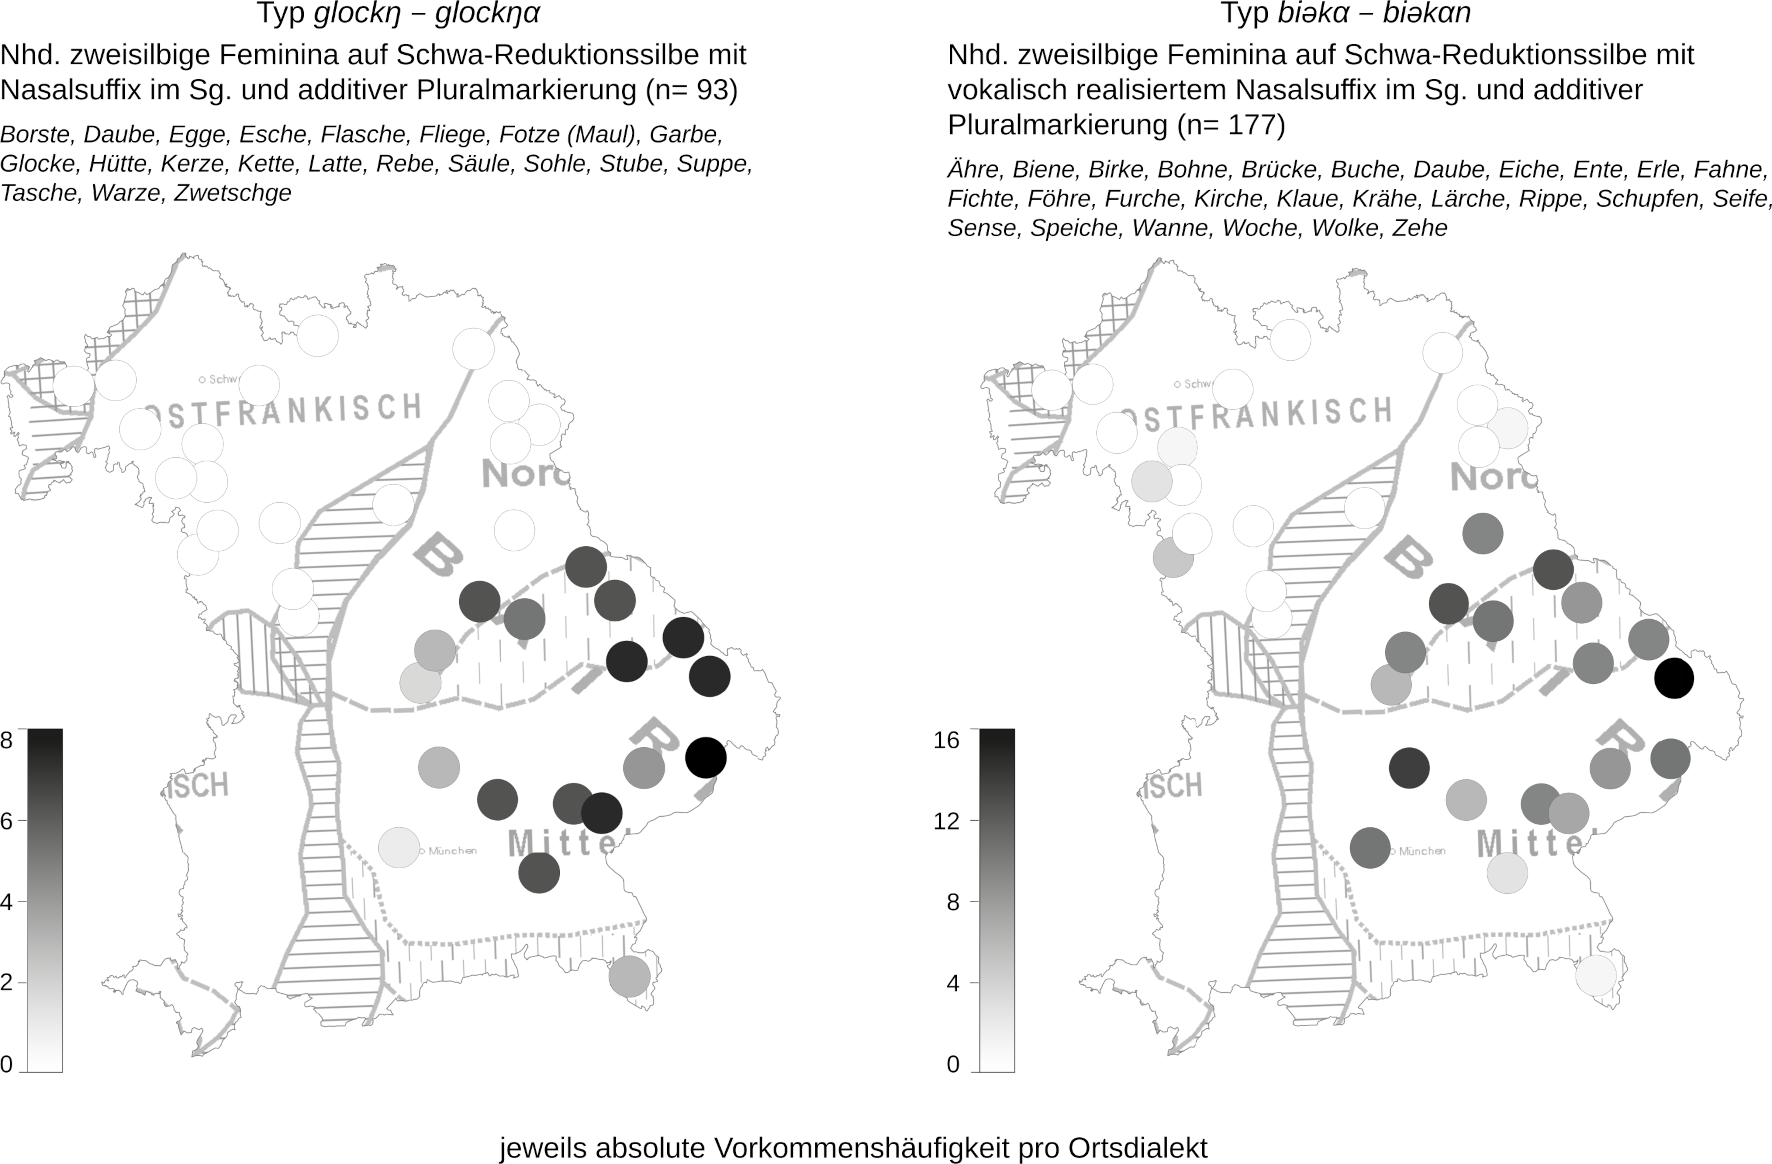
\includegraphics[width=\textwidth]{figures/Karte4.png}
\caption{Chloroplethkarten mit absoluter Vorkommenshäufigkeit additiver Pluralmarkierung bei nhd. zweisilbigen Feminina mit Schwa-Reduktionssilbe ($n=270$)}
\label{map:4}
\end{map}

\citet[131--132]{Mauser2000} zeigt in seiner Apparent-time-Studie für den bair. Dialekt des Salzburger Lungaus, dass die „innovativeren“ numerusdistinkten Formen mit Tiefschwa-Suffix in der älteren Sprechergeneration zu finden sind (z.\,B. \textit{ˈfaɪχtn̩} -- \textit{ˈfaɪχtnɐ} ‚Fichte‘, \textit{ˈloɪb̥m̩} -- \textit{ˈloɪb̥mɐ} ‚Loipe‘), während die jüngere Generation die „konservativeren“ synkretischen Formen verwendet. \citet[132]{Mauser2000} erklärt diesen Befund mit der stärkeren Normorientierung der jüngeren Sprechergeneration, die den „potentiellen Wandel“ blockiere (siehe auch \citealt[216]{Mauser1998a}). \citet[187--188]{Wildfeuer2001} kann in seiner Apparent-time-Studie eines mittelbair. Dialekts indes keine Tendenz zum Aus- oder Abbau der additiven Numerusmarkierung \textit{n}{}-erweiterter Feminina finden.\footnote{Bemerkenswert ist aber, dass auch \citet[218]{Wildfeuer2001} der jüngeren Sprechergeneration trotz einiger Um- und Abbautendenzen bei einzelnen Phänomenen „deutlich konservative Züge“ attestiert.}\largerpage[2]

\begin{sloppypar}
Der zweisilbigen Singularform der \textit{n}{}-erweiterten Feminina gleicht synchron die Struktur der zweisilbigen Maskulina mit Reduktionssilbe -\textit{en} (Typ \textit{Haufen}). Auch hier wird die Reduktionssilbe im gesamten UG in Abhängigkeit vom Stammauslaut als Nasal oder vokalisch realisiert, doch nur im südlichen Nordbair. und im Mittelbair. finden sich bei vokalisch realisierter Reduktionssilbe -\textit{α} additive Pluralformen mit Nasalsuffix: \teuthoo{ho.<v5A}{hôͅv̩α} -- \teuthoo{ho.<vAn}{hôͅvαn} ‚Hafen‘ (mittelbair. Grafenau), \teuthoo{ha4<o4v\%A}{hậọv͈α} -- \teuthoo{ha4<o4<v\%An}{hậộv͈αn} ‚Haufen‘ (mittelbair. Rei\-schach), \teuthoo{k,\_a.rpfA}{k͓ʰaͅrpfα} -- \teuthoo{k\_arpfAn}{kʰarpfαn} ‚Karpfen‘ (nordbair. Kallmünz), \teuthoo{k\_uAxA5}{kʰuαxα̩} -- \teuthoo{k\_uAxAn}{kʰuαxαn} ‚Kuchen‘ (nordbair.-mittelbair. Blaibach, vgl. \citealt[128 und 160]{Rowley1997}). \sectref{sec:8.3.3.1} wird zeigen, dass für die \textit{n}{}-Suffigierung bei femininen und maskulinen CVCV-Strukturen auf -\textit{α} von einem dialektraumspezifischen, produktiven Pluralbildungsmuster ausgegangen werden kann (siehe auch \sectref{sec:8.2.1} zur Deklination der historisch schwachen Maskulina in den rezenten Dialekten).
\end{sloppypar}

Daneben stellt auch die Abfolge aus Nasal im Stammauslaut und \textit{α}{}-Suffix in Pluralformen des Typs \teuthoo{s\#tu.mA}{štuͅmα} ein produktives Pluralbildungsmuster im Mittelbair. dar (inklusive der Übergangsgebiete zum Nord- und Südbair., siehe \citealt[166]{Mauser1998a}, \citealt[425]{Rowley1990b}, \citealt[128 und 160]{Rowley1997}, \citealt[58]{SMF7}, vgl. \citealt[§46h12]{Kranzmayer1956}). Diese Pluralformen mit Nasal+\textit{α} finden sich dabei auch für Feminina, deren Singularform kein Nasalsuffix aufweist, z.\,B. \teuthoo{nôo(+u(+d5}{n{\aufstrih}õ\klammerobenpost{}ũ\klammerobenpost{}d̩} -- \teuthoo{nôo(+u(+nA}{n{\aufstrih}õ\klammerobenpost{}ũ\klammerobenpost{}nα} ‚Naht‘ (nordbair. Oberdolling) und \teuthoo{s5a4<i:}{s̩ậi{\doubleogonek}} -- \teuthoo{s5a4<i:nA}{s̩ậi{\doubleogonek}nα} ‚Säule‘ (mittelbair.-südbair. Ramsau, siehe Abschnitte~\ref{sec:7.1.2.3.2} und \ref{sec:8.3.3.1}).\footnote{\citet[117]{Zehetner1985} nennt etwa noch die Form \textit{Frauna} (neben \textit{Frauan}) ‚Frauen‘, bei \citet[166]{Mauser2000} findet sich \textit{d̥ʀɔˑxd̥} -- \textit{ˈd̥ʀɔˑxt̺nɐ} ‚Tracht‘.}

Neben diesen Belegen für eine produktive Plural-Outputstruktur bei den Feminina finden sich nur für das schwache Maskulinum \textit{Bube} Pluralformen dieses Typs im nordbair.-mittelbair. Übergangsgebiet, vgl. \teuthoo{bo:u}{bo{\doubleogonek}u} -- \teuthoo{bo:umA}{bo{\doubleogonek}umα} -- \teuthoo{midn@}{midn̥} \teuthoo{bo:umAn}{bo{\doubleogonek}umαn} in Blaibach (vgl. \citealt[§38]{Kollmer1985}). Laut \citet[138]{Rowley1997} ist das \textit{α}{}-Suffix hier eine Form fakultativer Pluralmarkierung, die in dieser Form im südlichen Nordbair. und Mittelbair. sonst nur bei \textit{n}{}-erweiterten Feminina zu finden ist (\sectref{sec:9.2}). Diachron ist die Doppelsuffigierung das Ergebnis eines Assimilationsprozesses von Stammauslaut und Nasalsuffix in der Pluralform \textit{buben > bum}, die hier als „neue Grundgröße“ \citep[192]{Zehetner1978} die Basis für die „potenzierte“ additive Markierung bildet. Da auch nicht-assimilierte Singularformen wie \textit{lodn} ‚Latten‘ den Plural additiv mit Tiefschwa-Suffix bilden (Pl. \textit{lodna}), sieht \citet[123]{Steininger1994} Zehetners Argument einer Reanalyse der Wortstruktur infolge der Assimilation kritisch, die Ursache für die Suffigierung bestehe vielmehr darin, „daß der Pl. vom Sg. eindeutig unterschieden wird.“

\subsubsection{Suffixalternation}\label{sec:7.1.1.4}\largerpage
Für historisch zweisilbige Feminina der \textit{n}{}- und \textit{ô}{}-Deklination, die in der rezenten Singularform Nasalsuffix aufweisen, finden sich im mittelbair. Teil des UGs Belege für formal distinkte Singular- und Pluralformen, die sich im Suffix unterscheiden: \teuthoo{brukn}{brukn} -- \teuthoo{brukAn}{brukαn} ‚Brücke‘ (mittelbair. Wolfersdorf), \teuthoo{A}{α} \teuthoo{woi.k-N}{woiͅk{}͐ŋ} -- \teuthoo{woi.kA4n}{woiͅkα̣n} \teuthoo{E.}{əͅ} \teuthoo{hi9.me}{hi\klammeruntenpost{}ͅme} ‚Wolke/Wolken am Himmel‘ (mittelbair. Inning am Holz). Als additives Pluralmarkierungsverfahren stellen diese Suffixalternationen einen Grenzfall dar: Zwar sind -\textit{n} und \textit{{}-αn} jeweils segmentierbar, jedoch erfolgt die Numerusdifferenzierung nicht in Form einer Verkettung von Stammmorphem und Flexiv, als vielmehr in Form eines Austauschs der Morpheme. Die Form des Pluralsuffixes -\textit{αn} sowie die Pluralform als Ganzes entsprechen dabei der spezifischen Outputstruktur der Feminina im Bair. (vgl. \sectref{sec:8.3.3.1}).

Insgesamt finden sich im Korpus nur zwölf Belege dieser Suffixalternation \mbox{-\textit{n}} > -\textit{αn}, davon drei im mittelbair. Wolfersdorf und zwei im mittelbair. Waldhof. Die Alternation scheint im Mittelbair. insgesamt nur vereinzelt zu finden sein ($n=8$, vgl. \citealt[Karte 85 ‚Esche‘]{SOB4}). \citet[§572--573]{Schmeller1821} nennt einzelne Beispiele von Nominativ-Singular- und Pluralformen mit dem Suffix {}-\textit{ən} \mbox{(-\textit{αn})}, \citet[142]{Rowley1997} führt nur Belege für eine Alternation des Suffixes zwischen Nom. und Dat.Pl. in einem Gebiet im nördlichen Nordbair. und im Ofr. in der südlichen Fränkischen Schweiz an: Nom.Pl. \teuthoo{ga4rtn}{ɡạrtn} -- Dat.Pl. \teuthoo{ga4rtan}{ɡạrtan} ‚Gärten‘ (nordbair. Tirschenreuth), Nom.Pl. \teuthoo{ogsn}{oɡsn} -- Dat.Pl. \teuthoo{ogsan}{oɡsan} ‚Ochsen‘ (ofr. Pretzfeld), Nom.Pl. \teuthoo{gho.tSn}{ɡhoͅtʃn} -- Dat.Pl. \teuthoo{gho.tSan}{ɡhoͅtʃan} ‚Katzen‘ (nordbair. Neualbenreuth, vgl. \sectref{sec:7.2.1}). Suffixalternationen bei \textit{n}{}-erweiterten Feminina finden sich unterdessen auch im südlichen Arbeitsgebiet des SBS (d.\,h. im Schwäb. und mittelbair.-schwäb. Übergangsgebiet) in Form einer „geringen Aufhellung, die aber den Sprechern deutlich bewusst ist“ \citep[64]{Freudenberg1959}, von -\textit{ə} zu -\textit{α}/\textit{a}: \teuthoo{A}{α} \teuthoo{nu.<iE@}{nûͅiə̥} \teuthoo{glo4kE}{ɡlọkə} -- \teuthoo{nu.<iE@}{nûͅiə̥} \teuthoo{glo4ka}{ɡlọka} ‚(eine) neue Glocke(n)‘ im schwäb. Bernbeuren (vgl. \mapref{map:33}, \citealt[8]{Rowley1994}, \citealt[261--262 sowie Karten 105--113]{SBS9.1}).

Ein weiterer Fall von Suffixalternation findet sich im Ofr., wo Diminutiva gebietsweise unterschiedliche Diminutivsuffixe in der Singular- und Pluralform aufweisen: -\textit{la}/-\textit{le} im Singular, -\textit{li}/-\textit{liX} im Plural, z.\,B.: \teuthoo{ma42dlA}{mạ̄dlα} -- \teuthoo{ma42dJi.}{mạ̄d{\lkreis}iͅ} ‚Mädchen‘ (ofr. Burgbernheim), \teuthoo{mu?glE}{müɡlə} -- \teuthoo{mu?gli.c}{müɡliX} ‚Mücke‘ (ofr. Gemünden am Main, vgl. \citealt[Karte 34]{Rowley1997}, \citealt[22--23 und Karte 45]{SMF7}, \citealt[Karte 54]{SUF3}, \citealt{WA}-Karte 381 „Apfelbäumchen“). Numerusdifferenzierung findet hier an der Schnittstelle von Flexionsmorphologie und Wortbildung statt, sodass sich die Frage stellt, in welchem Bereich der Morphologie die einzelnen Diminutiv-Flexionsformen in der Analyse stärker verortet werden.

Historisch werden die verschiedenen Suffixe der Singular- und Pluralformen auf verschiedene Derivationssuffixe zurückgeführt:

\begin{itemize}
\item Die Suffixformen -\textit{la}/-\textit{le} im Singular gehen auf das Diminutivsuffix mhd. -\textit{lîn} zurück, das im UG weitestgehend mit elidiertem auslautendem Nasal erscheint.
\item Die Pluralsuffixe -\textit{li}/-\textit{liX} könnten auf ein kollektivierendes Derivationssuffix zurückgehen (\citealt[§596--606]{Schmeller1821}, \citealt[112]{Wrede1908}, vgl. \citealt[24--25]{Rowley1994}, \citealt[194--195]{SMF7}).
\item Im Nordbair. und im ofr.-nordbair. Übergangsgebiet erscheint im Plural das Suffix -\textit{la}, das ebenfalls auf ein Kollektivsuffix (-\textit{lach}) zurückgeht (\citealt[22--24]{Rowley1994}, vgl. \citealt[1253]{Seebold1983}).
\end{itemize}

Wenngleich die Diminutiva historisch auf unterschiedliche Derivationssuffixe zurückgehen, wird synchron in einem Streifen im östlichen Ofr. formal nicht zwischen Singular und Plural unterschieden: Typ \teuthoo{A}{α} \teuthoo{va94sla94}{va\klammeruntenpost{}̣sla\klammeruntenpost{}̣} -- \teuthoo{va94sla94}{va\klammeruntenpost{}̣sla\klammeruntenpost{}̣} ‚Fass‘ (ofr. Ahorn, vgl. \citealt[Karte 33]{Rowley1997}, \citealt[Karten 63.1/2]{Steger1968}). Im Nordbair. (inklusive Übergangsgebiete) ist dagegen der Typ \teuthoo{bri.kl@}{briͅkl̥} -- \teuthoo{bri.klA}{briͅklα} ‚Brücke‘ (nordbair. Groschlattengrün) verbreitet mit Diminutivsuffix -\textit{(ə)l} im Singular und -\textit{la} im Plural. Daneben finden sich synkretische Formen und Formen mit Nasalsuffix, und zwar teilweise nebeneinander, vgl. die Formen \teuthoo{a42dAl@}{ạ̄dαl̥} -- \teuthoo{a42dAlA}{ạ̄dαlα}, \teuthoo{a42dAln}{ạ̄dαln}, \teuthoo{a42dAl}{ạ̄dαl} ‚Ader‘ im nordbair.-mittelbair. Zwiesel. \citet[136]{Rowley1997} zufolge stellen die Plurale auf -\textit{a} die älteren, jene auf -\textit{n} die jüngeren Formen dar.

\begin{sloppypar}
In der Klassifikation des SMF werden Diminutivbildungen des Typs \teuthoo{bri.kl@}{briͅkl̥} -- \teuthoo{bri.klA}{briͅklα} zur Pluralmarkierung durch unterschiedliche Diminutivsuffixe gezählt und damit stärker der Wortbildung zugerechnet (\citealt[204]{SMF7}). Alternativ zu dieser Klassifikation, die die diachrone Entwicklung des Diminutivsuffixes bewahrt, analysiere ich diesen Typus im Sinne einer synchronen Klassifikation als additive Pluralmarkierung mit Nasal- bzw. Tiefschwa-Suffix. Auch wenn die rezenten Diminutivformen diachron auf eine Alternation der Suffixe im Singular und Plural zurückgehen, scheint diese Analyse hier vorteilhafter, denn sie  ermöglicht es, die Formen \teuthoo{a42dAlA}{ạ̄dαlα} und \teuthoo{a42dAln}{ạ̄dαln} gleichermaßen als additive Plurale zu klassifizieren: Sowohl \textit{α}{}- als auch Nasalsuffix gehören zum dialektalen Pluralmarkerinventar in diesem Teil des UGs und stellen damit produktive Pluralbildungsverfahren dar (vgl. \citealt[1199]{Dingeldein1983}).
\end{sloppypar}

\subsection{Stammaffizierende Markierung}
\label{sec:7.1.2}
Zur stammaffizierenden Markierung zählen jene Pluralmarkierungsverfahren, die nicht in einer Verkettung von Morphemen bestehen, sondern die die lautliche Form des Stammes verändern. In den untersuchten Dialekten gehören hierzu Markierungsstrategien, die den Vokalismus oder Konsonantismus des Stammes affizieren, subtraktive Verfahren und kombinierte Markierungen (d.\,h. die kumulative Kombination verschiedener additiver und/oder stammaffizierender Verfahren). Morphologie vollzieht sich hier an der Schnittstelle zum phonologischen System: Stammaffizierende Markierung ist das Ergebnis phonologisch bedingter Alternationen im Flexionsparadigma, die teilweise historische phonologische Prozesse konservieren, teilweise aber auch in den phonologischen Systemen der rezenten Dialekte wirksam sind. Die diachrone Perspektive zeigt hier auf, inwiefern das phonologische System der einzelnen Dialekte Voraussetzung für spezifische morphophonologische Verfahren ist. So sind in Dialekten, die zwar die Einsilberdehnung vollzogen, aber keine Lenis-Fortis-Oppositionen im phonologischen System bewahrt haben, innerparadigmatische Alternationen der Vokalquantität morphologisiert. Dialekte mit Lenis-Fortis-Kontrasten hingegen haben diese neben oder in Kombination mit Quantitätskontrasten funktionalisiert.

Ziel der folgenden Kapitel ist es, das konkrete Inventar stammaffizierender Pluralmarkierungsstrategien auszuweisen und gleichzeitig zu zeigen, inwiefern sie durch dialektspezifische Lautentwicklungen und phonologische Prozesse bedingt sind. Im Einzelfall wird zu entscheiden sein, ob rezente innerparadigmatische Alternationen primär phonologisch bedingt sind, ob sie eine lexikalisierte morphophonologische Alternation darstellen oder ob sie als morphologische Markierungsstrategien funktionalisiert und produktiv sind.

\subsubsection{Kontraste der Vokalqualität}
\label{sec:7.1.2.1}
Kontraste der Vokalqualität stellen im UG ein ausgesprochen frequentes Pluralmarkierungsverfahren dar. Neben dem Umlaut als dem „allgemeinsten Bildungsmittel des Plurals“ \citep[1086]{Lüssy1983} in den hd. Dialekten finden sich der umlautähnliche Diphthongwechsel bei Lexemen mit dem Stammvokal mhd. \textit{ei} (\sectref{sec:7.1.2.1.2}) sowie innerparadigmatische Wechsel der Zungenhöhe (\sectref{sec:7.1.2.1.3}). Auf diachrone phonologische Entwicklungen des Vokalsystems wird nur dann im Detail zurückgegriffen, wenn es für die Fragestellung relevant ist. Für eine detaillierte Aufführung der historischen phonologischen Entwicklungen im Vokalismus in den einzelnen Tiefenbohrungspunkten sei an dieser Stelle auf die relevanten BSA-Bände verwiesen.

\subsubsubsection{Umlaut}
\label{sec:7.1.2.1.1}
Der Umlaut stellt als „Paradebeispiel“ (\citet[57]{Rowley1997} eines innerparadigmatischen Vokalwechsels die frequenteste Form stammaffizierender Morphologie im UG dar. Historisch bezeichnet der Umlaut die assimilatorische Palatalisierung (auch Frontierung, vgl. etwa \citealt{Wiese1987}) eines hinteren Vokals unter Einfluss eines /i/ oder /j/ in der Folgesilbe (vgl. \citealt[194--199]{Schirmunski1962}, \sectref{sec:3.1.1}). Auch synchron entspricht der Umlaut einem Wechsel von velarem zu palatalem Vokal, das spezifische Wechselmuster des Umlauts besteht nach \citet[57]{Rowley1997} dabei idealiter in der „vollen“ Korrelation der Zungenhöhe. Das Prinzip der Zungenhöhenkorrelation stelle dabei auch diachron ein stabiles Merkmal dar, da die phonologischen Entwicklungen der Vokalsysteme der nordostbayrischen Dialekte die vorderen und hinteren Vokalreihen gleichermaßen betreffe oder die Korrelation im Falle von mhd. \textit{a}, \textit{â} durch Ausgleich hergestellt werden könne (\citealt[57--66]{Rowley1997}, vgl. \citealt[47]{Steger1968}). Zu einer Aufhebung der „vollen“ Zungenhöhenkorrelation führt dagegen die Dehnung des Basisvokals infolge der Einsilberdehnung, da der Quantitätskontrast als weiteres phonologisches Merkmal hinzukommt \citep[67]{Rowley1997}.

\citet[117]{Rowley1997} bestätigt für die Dialekte Nordostbayerns den Befund \citegen{Moulton1971} für das Schweizerdeutsche: Das morphophonologische Prinzip des Umlauts besteht in der Alternation zwischen velarem und palatalem Vokal und damit in der Modulation der Merkmalsopposition [±palatal]. Analoge Umlautformen sind stets korrelierende Umlaute, d.\,h. die Merkmalsopposition [±palatal] ist morphologisiert \citep[117]{Rowley1997}. Von korrelierenden Umlauten sind nach \citet[118]{Rowley1997} teilkorrelierende Umlaute zu unterscheiden, die neben der Modulation des Merkmals [±palatal] Variation in einem weiteren phonologischen Merkmal aufweisen (nämlich Rundung, Öffnung oder Vokalquantität). Nicht-korrelierende Umlaute weichen daneben in gleich mehreren phonologischen Merkmalen ab.

Die folgenden Detailanalysen mit Bezug auf das mhd. Vokalsystem werden zeigen, dass die Umlautrelationen dialektspezifisch sind und im interdialektalen Vergleich variieren. Zu unterscheiden sind Systeme, in denen historisch eine Reduktion der Vokalalternanzen stattgefunden hat, und Systeme, in denen diachron eine lautgesetzlich bedingte Ausdifferenzierung der Vokalalternanzen erfolgt ist. Die Oppositionen in den rezenten Vokalsystemen und damit auch die dialektalen Umlautmöglichkeiten sind jeweils das Ergebnis historischer phonologischer Prozesse, die den Stammvokalismus affizieren (in diesem Zusammenhang insbesondere Rundung/Entrundung, Monophthongierung/Diphthongierung), von Aufhebung von Oppositionen (d.\,h. Zusammenfall von Lauten) und von Phonemspaltungen (vgl. \citealt[1084]{Lüssy1983}, \citealt[117]{Rowley1997}, \citealt[200--202]{Schirmunski1962}, \citealt[1046]{Wiesinger1983d}).

\subsubsubsubsection{Rezente Umlautentsprechungen vor dem Hintergrund des mhd. Protosystems}
In \figref{fig:4} werden die rezenten Umlautentsprechungen für fünf exemplarische Ortsdialekte im ofr. Rundungsgebiet (Erlabrunn), im ofr. Entrundungsgebiet (Wilhermsdorf), im Nordbair. (Windischeschenbach) und im Mittelbair. (Kirchensur) getrennt für die mhd. Vokalreihen dargestellt. Die Anordnung der Umlautmöglichkeiten entspricht der Anordnung im Vokaltrapez, d.\,h. die velaren Basisvokale sind in den einzelnen Grafiken rechts zu finden, die palatalen Umlautvokale links. Basis- und Umlautvokale wurden nach Quantität differenziert. Anders als \citet[1049]{Wiesinger1983d} setze ich keine quantitätslosen Vokalsysteme für das Nord- und Mittelbair. an, da Quantitäts- und Lenis-Fortis-Kontraste unabhängig voneinander realisiert werden können (vgl. \sectref{sec:7.1.2.3.1}).




\begin{sidewaysfigure}
\small
\begin{tabularx}{\textwidth}{@{}Qp{2.5cm}p{2cm}>{\centering}p{3.5cm}p{2cm}@{}}
 & ofr.\newline Wilhermsdorf & ofr.\newline Erlabrunn & nordbair.\newline Windischeschenbach   & mittelbair.\newline  Kirchensur \\
 \hline
%  \parbox[b]{4cm}{
 \textbf{mhd. i--ü--u, î--iu--û}\newline\footnotesize
  Fuchs, Hund, Nuss, Sohn, Strumpf, Stube, Turm, Wurm, Wurst, Wurzel; \newline
  Bauch, Faust, Haufen, Haus, Haut, Maul, Maus, Sau, Strauß, Zaun
%   }
    &
    \begin{tikzpicture}[baseline=(i.base),every node/.style={inner sep=0,outer sep=0}]
      \node(i){i\strut};
      \node(e)[below=0mm of i]{e \strut};
      \node(ea)[below=0mm of e]{eα \strut};
      \node(ae)[below=0mm of ea]{ae \strut};


      \node(u)[right=10mm of i]{u\strut};
      \node(o)[below=0mm of u]{o\strut};
      \node(oa)[below=0mm of o]{oα\strut};
      \node(ao)[below=0mm of oa]{ao\strut};

      \draw(i.east)--(u.west);
      \draw(e.east)--(o.west);
      \draw(ea.east)--(oa.west);
      \draw(ae.east)--(ao.west);
    \end{tikzpicture}
    &
    \begin{tikzpicture}[baseline=(ü.base),every node/.style={inner sep=0,outer sep=0}]
      \node(ü){ü\strut};
      \node(none1)[below=0mm of ü]{~\strut};
      \node(ö)[below=0mm of none1]{ö \strut};
      \node(öö)[below=0mm of ö]{\=ö \strut};
      \node(aü)[below=0mm of öö]{aü \strut};
      \node(ai)[below=0mm of aü]{ai \strut};


      \node(u)[right=10mm of i]{u\strut};
      \node(uu)[below=0mm of u]{\=u\strut};
      \node(o)[below=0mm of uu]{o\strut};
      \node(oo)[below=0mm of o]{\=o\strut};
      \node(ao)[below=2mm of oo]{ao\strut};

      \draw(ü.east)--(u.west);
      \draw[dotted,thick](ü.east)--(uu.west);
      \draw[dotted,thick](ö.east)--(u.west);
      \draw(ö.east)--(o.west);
      \draw(öö.east)--(oo.west);
      \draw[dotted,thick](ö.east)--(ao.west);
      \draw[dotted,thick](ö.east)--(oo.west);
      \draw(aü.east)--(ao.west);
      \draw(ai.east)--(ao.west);
    \end{tikzpicture}
    &
    \begin{tikzpicture}[baseline=(i.base),every node/.style={inner sep=0,outer sep=0}]
      \node(i){i\strut};
      \node(iie)[below=0mm of i]{{\=\i}ǝ \strut};
      \node(none1)[below=0mm of iie]{~\strut};
      \node(aai)[below=0mm of none1]{\=ai \strut};
      \node(ai)[below=0mm of aai]{ai \strut};


      \node(u)[right=10mm of i]{u\strut};
      \node(uue)[below=0mm of u]{{\=u}ə\strut};
      \node(aa)[below=0mm of uue]{\={ạ}\strut};
      \node(aao)[below=0mm of aa]{\=ao\strut};

      \draw(i.east)--(u.west);
      \draw(iie.east)--(uue.west);
      \draw(aai.east)--(aao.west);
      \draw[dotted,thick](ai.east)--(aa.west);
      \draw[dotted,thick](ai.east)--(aao.west);
    \end{tikzpicture}
    &
      \begin{tikzpicture}[baseline=(i.base),every node/.style={inner sep=0,outer sep=0}]
      \node(i){i\strut};
      \node(ii)[below=0mm of i]{\=i \strut};
      \node(ae)[below=0mm of ii]{ae \strut};
      \node(aae)[below=0mm of ae]{\=ae \strut};


      \node(u)[right=10mm of i]{u\strut};
      \node(uu)[below=0mm of u]{\=u\strut};
      \node(ao)[below=0mm of uu]{ao\strut};
      \node(aao)[below=0mm of ao]{\=ao\strut};

      \draw(i.east)--(u.west);
      \draw(ii.east)--(uu.west);
      \draw(ae.east)--(ao.west);
      \draw(aae.east)--(aao.west);
      \draw[dotted,thick](i.east)--(uu.west);
      \draw[dotted,thick](ae.east)--(aao.west);
    \end{tikzpicture}\\
    \hline
\textbf{mhd. e--ö--o, ê--œ--ô}\newline\footnotesize
Bock, Boden, Borste, Dof, Dorn ,Forsch, Bbel, Horn, Joch, Knophf, Knoten, Kopf, Korb, Korn, Kfroph, Loch, Ofen, Rock, Schloss, Stock, Tochter, Tropf, Trog, Vogel, Zopf;\newline
Floh, Kloß, Lohn, Ohr &
    \begin{tikzpicture}[baseline=(i.base),every node/.style={inner sep=0,outer sep=0}]
      \node(e){e\strut};
      \node(ee)[below=0mm of e]{\=e \strut};
      \node(none1)[below=0mm of ee]{~ \strut};

      \node(o)[right=10mm of i]{o\strut};
      \node(oo)[below=0mm of o]{\=o\strut};
      \node(aa)[below=0mm of oo]{\=a\strut};

      \draw(e.east)--(o.west);
      \draw(ee.east)--(oo.west);
      \draw(ee.east)--(aa.west);
      \draw[dotted,thick](e.east)--(oo.west);
    \end{tikzpicture}
    &
    \begin{tikzpicture}[baseline=(i.base),every node/.style={inner sep=0,outer sep=0}]
      \node(ö){ö\strut};
      \node(none1)[below=0mm of ö]{~ \strut};
      \node(ööi)[below=0mm of none1]{\=öï\strut};
      \node(ööa)[below=0mm of ööi]{\=öα\strut};

      \node(o)[right=10mm of ö]{o\strut};
      \node(oo)[below=0mm of o]{\=o\strut};
      \node(oou)[below=0mm of oo]{\=ou\strut};
      \node(ooa)[below=0mm of oou]{\=oα\strut};

      \draw(ö.east)--(o.west);
      \draw(ööi.east)--(oou.west);
      \draw(ööa.east)--(ooa.west);
      \draw[dotted,thick](ö.east)--(oo.west);
      \draw[dotted,thick](ö.east)--(oou.west);
      \draw[dotted,thick](ö.east)--(ooa.west);
    \end{tikzpicture}
    &
    \begin{tikzpicture}[baseline=(ü.base),every node/.style={inner sep=0,outer sep=0}]
      \node(iie){\=iə\strut};
      \node(e)[below=0mm of iie]{e};
      \node(eea)[below=0mm of e]{{\=e}α  \strut};
      \node(eei)[below=0mm of eea]{\=ei \strut};
      \node(a)[below=0mm of eei]{ạ \strut};

      \node(uue)[right=10mm of i]{{\=u}ə\strut};
      \node(ooo)[below=2mm of uue]{\aufstrich\=oo\strut};
      \node(ooa)[below=2mm of ooo]{\=oα\strut};

      \draw(iie.east)--(uue.west);
      \draw(eea.east)--(ooa.west);
      \draw[dotted,thick](e.east)--(uue.west);
      \draw[dotted,thick](eei.east)--(ooo.west);
      \draw[dotted,thick](eei.east)--(ooa.west);
      \draw[dotted,thick](a.east)--(ooa.west);
    \end{tikzpicture}
    &
    \begin{tikzpicture}[baseline=(ü.base),every node/.style={inner sep=0,outer sep=0}]
      \node(i){i\strut};
      \node(none1)[below=0mm of i]{~\strut};
      \node(e)[below=0mm of none1]{e \strut};
      \node(ee)[below=0mm of e]{\=e \strut};

      \node(none2)[right=10mm of i]{~\strut};
      \node(uu)[below=0mm of none2]{\=u\strut};
      \node(o)[below=0mm of uu]{o\strut};
      \node(oo)[below=0mm of o]{\=o\strut};
      \node(oou)[below=0mm of oo]{\aufstrich\=ou\strut};

      \draw(e.east)--(o.west);
      \draw(ee.east)--(oo.west);
      \draw[dotted,thick](i.east)--(uu.west);
      \draw[dotted,thick](e.east)--(oo.west);
      \draw[dotted,thick](ee.east)--(oou.west);
    \end{tikzpicture}\\
    \textbf{mhd. a, â, ë, ä æ}\newline\footnotesize
    Acker, Apfel, Ast, Bach, Band, Bank, Blatt, Dach, Darm, Faden, Fass, Gabel, Gang, Gans, Garten, Glas, Grab, Grabene, Hafen, Hammer, Hand, Kalb, Kamm, Karren, Magd, Magen, Mann, Markt, Nacht, Nagel, Name, Rad, Sack, Schlag, Schnabel, Schwanz, Stadt, Stall, Start, Tag, Wade, Wagen, Wald, Wasen, Zahn;\newline
    Draht, Naht, Pfahl, Schaf, Straße
    &
    \begin{tikzpicture}[baseline=(i.base),every node/.style={inner sep=0,outer sep=0}]
      \node(e){e\strut};
      \node(ee)[below=0mm of e]{\=e \strut};

      \node(o)[right=10mm of e]{o\strut};
      \node(oo)[below=0mm of o]{\=o\strut};
      \node(a)[below=0mm of oo]{a\strut};
      \node(aa)[below=0mm of a]{\=a\strut};

      \draw(e.east)--(o.west);
      \draw(e.east)--(a.west);
      \draw(ee.east)--(oo.west);
      \draw(ee.east)--(aa.west);
      \draw[dotted,thick](e.east)--(oo.west);
    \end{tikzpicture}
    &
    \begin{tikzpicture}[baseline=(i.base),every node/.style={inner sep=0,outer sep=0}]
      \node(ö){ö\strut};
      \node(e)[below=0mm of ö]{e \strut};
      \node(ee)[below=0mm of e]{\=e \strut};
      \node(eei)[below=0mm of ee]{\=ei \strut};
      \node(ööa)[below=0mm of eei]{\=öα \strut};
      \node(eea)[below=0mm of ööa]{\=eα \strut};
      \node(a1)[below=0mm of eea]{\d{a} \strut};
      \node(aa1)[below=0mm of a1]{\=a \strut};


      \node(oo)[right=10mm of ee]{\=o\strut};
      \node(ooa)[right=10mm of ööa]{\=oα\strut};
      \node(a2)[right=10mm of a1]{a\strut};
      \node(aa2)[right=10mm of aa1]{\=a\strut};

      \draw(e.east)--(aa2.west);
      \draw(ee.east)--(oo.west);
      \draw(ee.east)--(aa2.west);
      \draw(ööa.east)--(ooa.west);
      \draw(eea.east)--(ooa.west);
      \draw(a1.east)--(a2.west);
      \draw(aa1.east)--(oo.west);
      \draw[dotted,thick](ö.east)--(oo.west);
      \draw[dotted,thick](ö.east)--(ooa.west);
      \draw[dotted,thick](ö.east)--(a2.west);
      \draw[dotted,thick](e.east)--(oo.west);
      \draw[dotted,thick](e.east)--(aa2.west);
      \draw[dotted,thick](eei.east)--(aa2.west);
      \draw[dotted,thick](a1.east)--(oo.west);
      \draw[dotted,thick](aa1.east)--(ooa.west);
    \end{tikzpicture}
    &
    \begin{tikzpicture}[baseline=(i.base),every node/.style={inner sep=0,outer sep=0}]
      \node(iie){\=iə\strut};
      \node(e)[below=0mm of iie]{e \strut};
      \node(ee)[below=0mm of e]{\=e \strut};
      \node(eei)[below=0mm of ee]{\=ei \strut};
      \node(a)[below=0mm of eei]{\d{a} \strut};
      \node(aa)[below=0mm of a]{\d{\=a} \strut};
%

      \node(none1)[right=10mm of iie]{~\strut};
      \node(o)[below=2mm of none1]{\=o\strut};
      \node(ooo)[below=0mm of o]{\aufstrich\=oo\strut};
      \node(ooa)[below=0mm of ooo]{\=oα\strut};
      \node(oa)[below=0mm of ooa]{\burgeroa\strut};

      \draw(ee.east)--(o.west);
      \draw(a.east)--(oa.west);
      \draw(aa.east)--(o.west);
      \draw[dotted,thick](iie.east)--(o.west);
      \draw[dotted,thick](e.east)--(o.west);
      \draw[dotted,thick](eei.east)--(ooo.west);
      \draw[dotted,thick](a.east)--(ooa.west);
    \end{tikzpicture}
    &
    \begin{tikzpicture}[baseline=(i.base),every node/.style={inner sep=0,outer sep=0}]
      \node(e){e\strut};
      \node(ee)[below=0mm of e]{\=e \strut};
      \node(a)[below=0mm of ee]{\d{a} \strut};
      \node(aa)[below=0mm of a]{\d{\=a} \strut};

      \node(o)[right=10mm of e]{o\strut};
      \node(oo)[below=0mm of o]{\=o\strut};
      \node(a2)[below=0mm of oo]{\k{a}\strut};

      \draw(e.east)--(o.west);
      \draw(e.east)--(a2.west);
      \draw(ee.east)--(oo.west);
      \draw(a.east)--(a2.west);
      \draw(aa.east)--(oo.west);
      \draw[dotted,thick](e.east)--(oo.west);;
    \end{tikzpicture}\\
    \textbf{mhd. ie--üe--uo}\newline\footnotesize
    Bruder, Fuß, Huhn, Hut, Krug, Kuh, Mutter, Pflug, Stuhl
    &
    \begin{tikzpicture}[baseline=(i.base),every node/.style={inner sep=0,outer sep=0}]
      \node(i){i\strut};
      \node(ii)[below=0mm of i]{\=i \strut};


      \node(u)[right=10mm of i]{u\strut};
      \node(uu)[below=0mm of u]{\=u\strut};

      \draw(i.east)--(u.west);
      \draw(ii.east)--(uu.west);
    \end{tikzpicture}
    &
    \begin{tikzpicture}[baseline=(i.base),every node/.style={inner sep=0,outer sep=0}]
      \node(üüe){\=üə\strut};
      \node(ö)[below=0mm of üüe]{ö \strut};
      \node(ööa)[below=0mm of ö]{\=öα \strut};


      \node(uue)[right=10mm of üüe]{\=uə\strut};
      \node(none1)[below=0mm of uue]{~\strut};
      \node(ooa)[below=0mm of none1]{oα\strut};

      \draw(üüe.east)--(uue.west);
      \draw(ööa.east)--(ooa.west);
      \draw[dotted,thick](ö.east)--(uue.west);
      \draw[dotted,thick](ööa.east)--(uue.west);
    \end{tikzpicture}
    &
    \begin{tikzpicture}[baseline=(i.base),every node/.style={inner sep=0,outer sep=0}]
      \node(none1){~\strut};
      \node(eei)[below=0mm of none1]{\=ei \strut};
      \node(ei)[below=0mm of eei]{ei \strut};

      \node(ööu)[right=10mm of üüe]{\aufstrich\=öu\strut};
      \node(oou)[below=0mm of ööu]{\aufstrich\=ou\strut};

      \draw(eei.east)--(oou.west);
      \draw[dotted,thick](eei.east)--(ööu.west);
      \draw[dotted,thick](ei.east)--(ööu.west);
    \end{tikzpicture}
    &
    \begin{tikzpicture}[baseline=(i.base),every node/.style={inner sep=0,outer sep=0}]
      \node(none1){~\strut};
      \node(iia)[below=0mm of none1]{\=iα \strut};

      \node(ua)[right=10mm of none1]{uα\strut};
      \node(uua)[below=0mm of ua]{\=uα\strut};

      \draw(iia.east)--(uua.west);
      \draw[dotted,thick](iia.east)--(ua.west);
    \end{tikzpicture}
    \\
    \textbf{mhd. ei--öu--ou}\newline\footnotesize
    Baum, Reifen
    &
    \begin{tikzpicture}[baseline=(i.base),every node/.style={inner sep=0,outer sep=0}]
      \node(e){e\strut};
      \node(a)[right=10mm of e]{a\strut};
      \draw(e.east)--(a.west);
    \end{tikzpicture}
    &
    \begin{tikzpicture}[baseline=(i.base),every node/.style={inner sep=0,outer sep=0}]
      \node(ö){ö\strut};
      \node(aa)[right=10mm of ö]{\=a\strut};
      \draw(ö.east)--(aa.west);
    \end{tikzpicture}
    &
    \begin{tikzpicture}[baseline=(i.base),every node/.style={inner sep=0,outer sep=0}]
      \node(ai){âi\strut};
      \node(a)[right=10mm of ai]{\d{a}\strut};
      \draw[dotted,thick](ai.east)--(a.west);
    \end{tikzpicture}
    &
    \begin{tikzpicture}[baseline=(i.base),every node/.style={inner sep=0,outer sep=0}]
      \node(ea){eα};
      \node(oa)[right=10mm of ea]{oα\strut};
      \draw(ea.east)--(oa.west);
    \end{tikzpicture}\\



\end{tabularx}
  \caption{Rezente Umlautentsprechungen in exemplarischen Ortsdialekten mit mhd. Bezugssystem ($n=342$)\label{fig:4}}
\end{sidewaysfigure}

Die Umlautvokale unterscheiden sich in jenen Dialekten, in denen die Rundung der mhd. Bezugsvokale bewahrt wurde, von jenen, in denen Entrundung eingetreten ist, z.\,B. mhd. \textit{o}/\textit{ö} in \teuthoo{khôo.<ubv}{kh{\aufstrih}ôͅubv} -- \teuthoo{kho?bv}{khöbv} ‚Kopf‘ im ofr. Erlabrunn vs. \teuthoo{k\_o94bv5}{kʰo\klammeruntenpost{}̣bv̩} -- \teuthoo{khÔe:bv5}{kh{\doppelaufstrih}e{\doubleogonek}bv̩} im ofr. Wilhermsdorf. Entrundung der palatal-gerundeten Vokale findet sich im größten Teil des UGs, bewahrt ist Rundung im Unterofr. bis hinein in den Henneberger Raum und das Osthessische.\footnote{Vgl. \citet[67--68 und Karte 13]{Rowley1997}, \citet[204--208]{Schirmunski1962}, \citet[41--43 und Karten 22/31]{Steger1968}, \citet[1103]{Wiesinger1983e} sowie \citealt{WA}-Karte 465 „Häuser“.} Im Entrundungsgebiet werden die mhd. Umlautvokale \textit{ö}, \textit{ü}, \textit{iu} usw. ungerundet realisiert und sind mit mhd. \textit{e}, \textit{i}, \textit{î} usw. zusammengefallen, vgl. mhd. \textit{o}/\textit{ö} in \teuthoo{v5ro42s\#}{v̩rọ̄š} -- \teuthoo{v5re?S'}{v̩rëʃ̌} ‚Frosch‘ vs. mhd. \textit{a}/\textit{e} in \teuthoo{gða.ns}{ɡ̩aͅns} -- \teuthoo{gðens}{ɡ̩ens} ‚Gans‘ im mittelbair. Kirchensur (vgl. \citealt[§4a4]{Kranzmayer1956}, \citealt[1102]{Wiesinger1983e}).

In Rundungsdialekten finden sich gerundete Vorderzungenvokale als Basisvokale in nur wenigen Lexemen; wesentlich frequenter sind sie als Umlautprodukte in Flexionsformen, weshalb sie „deutliche Exponenten“ \citep[68]{Rowley1997} flexivischer Information darstellen. In diesen Dialekten kann Rundung in Kombination mit dem Umlaut als morphophonologischer Marker auch bei historisch palatal-ungerundeten Vokalen auftreten. Der palatal-gerundete Umlautvokal \textit{ö} (neben der diphthongischen Variante \teuthoo{o?"A}{ȫα}) findet sich in den Rundungsdialekten für alle historischen Vokalreihen, und zwar auch „an historisch unberechtigter Stelle“ \citep[68]{Rowley1997}. Dies gilt nach \citet[1103]{Wiesinger1983e} vor allem in der phonologischen Umgebung von Konsonanten mit Lippenrundung (\textit{b}/\textit{p}, \textit{w}, \textit{f}, \textit{š} und Affrikate \textit{bf}/\textit{pf}), beispielsweise bei \teuthoo{a.bv5l@}{aͅbv̩l̥} -- \teuthoo{o?bv5l@}{öbv̩l̥} -- Dim. \teuthoo{o?bv5ElA}{öbv̩əlα} ‚Apfel‘ (ofr. Krum) oder \teuthoo{a}{a} \teuthoo{bvo2L@}{bvōL̥} -- \teuthoo{bvo"?L}{bvȫL} ‚Pfahl‘ (ofr. Ahorn), daneben aber auch \teuthoo{dro.2Ed}{drōͅəd} -- \teuthoo{dro"?.Ed}{drȫͅəd} ‚Draht‘ (ofr. Stadtschwarzach), als nicht-korrelierender Umlaut in \teuthoo{ma94<o\$l}{ma\klammeruntenpost{}̣̂o̤l} -- \teuthoo{mo?9.lE.}{mö\klammeruntenpost{}ͅləͅ} -- Dim. \teuthoo{mo?9.lE.}{mö\klammeruntenpost{}ͅləͅ} ‚Maul‘ (ofr. Erlabrunn) oder als analogischer Umlaut in \teuthoo{do94An}{do\klammeruntenpost{}̣αn} -- \teuthoo{do?.Enê}{döͅən{\burgereshwa}} ‚Dorn‘ (ofr. Ahorn, vgl. \citealt[88--89]{Kemmeter1924}, \citealt[42]{Steger1968}).\footnote{Auch in den von \citet[30]{Niederlöhner1937} angeführten Beispielen der Realisierung von mhd. \textit{e}/\textit{ä} in (historisch) geschlossenen Silben als [ö] im Coburger Raum (Tiefenbohrungspunkt Ahorn) entspricht die lautliche Umgebung stets Konsonanten mit Lippenrundung, z.\,B. \textit{drøb} ‚Treppe‘, \textit{wøs} ‚Wespe‘ (vgl. \citealt[44]{Koß1967}).}

Diachron hat hier zum Teil eine Ausdifferenzierung der Vokalalternanzen stattgefunden: Für die synchronen Entsprechungen von mhd. \textit{a}, \textit{â} kommen die palatal-gerundeten neben den palatal-gespreizten Umlautvokalen vor, für mhd. \textit{o}/\textit{ö} und mhd. \textit{u}/\textit{ü} sind hingegen nur Alternationen von Velarvokal und gerundetem Umlautvokal belegt. Die synchronen Umlautentsprechungen in den ofr. Rundungsdialekten weisen damit ebenfalls „fast ablautähnliche Züge“ \citep[123]{Nübling2006} auf, wie sie Nübling für das Luxemburgische konstatiert: Die Vokalwechsel sind asymmetrisch und der Pluralvokal nicht in allen Fällen aus dem Singularvokal ableitbar (siehe auch \citealt[118]{Nübling2006}). Der Umlautvokal \textit{ö} erscheint als Marker der Pluralinformation dabei als stärker funktionalisiert, wie auch der Wechsel zwischen palatal-gespreiztem und palatal-gerundetem Vokal in der Plural- und der Diminutivform \teuthoo{de.?rv}{dëͅrv} -- \teuthoo{do?.rvEr}{döͅrvər} -- Dim. \teuthoo{de.?rvli.}{dëͅrvliͅ} ‚Dorf‘ im ofr. Hüttenheim belegt.

In den entrundeten Dialekten des Ofr. und Mittelbair. sind die Umlautrelationen (mit Ausnahme von mhd. \textit{a}, \textit{â}) weniger komplex, die Zuordnung von Basis- und Umlautvokal entspricht einer 1:1-Zuordnung. Da innerparadigmatische Vokalquantitätskontraste in diesen Dialekten ebenfalls morphologisiert sind, finden sich neben den korrelierenden Umlauten regelmäßig teilkorrelierende Umlaute, die sich im Merkmal der Palatalität und in der Vokalquantität unterscheiden. Die Umlautentsprechungen des Nordbair., hier exemplarisch Win\-discheschenbach, ähneln im Prinzip diesen Wechselmustern, allerdings ist hier eine stärkere Ausdifferenzierung der Umlautvokale zu beobachten. Die rezenten Entsprechungen sind in ihrer Distribution durch dialektspezifische historische Entwicklungen und durch die phonologische Umgebung konditioniert, wie weiter unten gezeigt wird. Der „ablautähnliche“ Charakter der Umlautmöglichkeiten des Nordbair. ist damit ererbt, wie exemplarisch an den Umlautentsprechungen für mhd. \textit{a}, \textit{â} zu sehen ist.

\vfill
\begin{table}[H]
\small
\begin{tabularx}{\textwidth}{QQQQQ}
\lsptoprule
& ofr. Erlabrunn & ofr. Wilhermsdorf & nordbair. Windisch\-eschenbach & mittelbair.

Kirchensur\\
\midrule
mhd. \textit{â}

(‚Draht‘) & \teuthoo{dro.2Ad5\_}{drōͅαd̩ʰ} -- \teuthoo{dro"?.Ad5\_}{drȫͅαd̩ʰ} & \teuthoo{dro:2d5\_}{dro{\doubleogonek}̄d̩ʰ} -- \teuthoo{dre.2d5\_}{drēͅd̩ʰ} & \teuthoo{drôo.2>o4d}{dr{\aufstrih}ō̂ͅọd} -- \teuthoo{dre<.i.d5\_}{drêͅiͅd̩ʰ} & \teuthoo{dro.2d}{drōͅd} -- \teuthoo{dra24d}{drạ̄d}\\
\tablevspace
mhd. \textit{a} in Dehnung (‚Glas) & \teuthoo{gla9.2s}{ɡla\klammeruntenpost{}̄ͅs} -- \teuthoo{gl{\textasciitilde}ôe9.<isEr}{gl{\aufstrih}eͅisər} -- \teuthoo{gla42slA94}{ɡlạ̄slα\klammeruntenpost{}̣} & \teuthoo{glo9.2s5}{ɡlo\klammeruntenpost{}̄ͅs̩} -- \teuthoo{gle942sE.}{ɡle\klammeruntenpost{}̣̄səͅ} -- \teuthoo{gle942sJA94}{ɡle\klammeruntenpost{}̣̄s{\lkreis}α\klammeruntenpost{}̣} & \teuthoo{glo24s}{ɡlọ̄s} -- \teuthoo{gli“EsA}{ɡlīəsα} -- \teuthoo{gla24sý@}{ɡlạ̄sɫ̥} & \teuthoo{glo.2s}{ɡlōͅs} -- \teuthoo{gle.2sA}{ɡlēͅsα} -- \teuthoo{gla42sl}{ɡlạ̄sl}\\
\tablevspace
mhd. \textit{a}

(‚Acker‘) & \teuthoo{a):gEr}{a\klammeruntenpost{}{\doubleogonek}ɡər} -- \teuthoo{a94gEr}{a\klammeruntenpost{}̣ɡər} & \teuthoo{a9.gE}{a\klammeruntenpost{}ͅɡə} -- \teuthoo{e.gE}{eͅɡə} & \teuthoo{åkA}{{\burgeroalpha}kα} -- \teuthoo{a\$kA}{a̤kα} & \teuthoo{o.kA}{oͅkα} -- \teuthoo{a4kA}{ạkα}\\
\lspbottomrule
\end{tabularx}
\caption{Dialektale Entsprechungen von mhd. \textit{a} mit erhaltener Kürze und in Dehnung, mhd. \textit{â} sowie den Umlautvokalen}
\label{tab:18}
\end{table}
\vfill\pagebreak

Mhd. \textit{â} und mhd. \textit{a} in Dehnung werden in den Dialekten des UG velarisiert (mit variierender Qualität des Verdumpfungsprodukts auf einem phonetischen Kontinuum \teuthoo{a2.}{āͅ}-\teuthoo{o.2}{ōͅ}-\teuthoo{o2}{ō}, bei mhd. \textit{â} im Nordbair. als Diphthong \teuthoo{o2.u}{ōͅu} bzw. \teuthoo{ôo2o}{{\aufstrih}ōo} in Windischeschenbach, vgl. \citealt{Gütter1971}: Karte 8). Im Bair. und im westlichen Ofr. wird auch mhd. \textit{a} bei erhaltener Kürze verdumpft, im übrigen Ofr. erfolgt keine qualitative Veränderung.{\interfootnotelinepenalty=10000\footnote{Vgl. \citet[§1b und Karte 1]{Kranzmayer1956}, \citet[57--58 und Karte 9]{Rowley1997}, \citet[200--201]{Schirmunski1962}, \citet[46--50 und Karte 2]{Steger1968}.}} Die Sekundär\-umlautvokale mhd. \textit{ä}, {\textit{æ}} werden im Unterofr. und im Bair. als heller \textit{ạ}{}-Laut, der Primär\-umlaut mhd. \textit{ë} hingegen als \textit{e}{}-Variante (\teuthoo{e.}{eͅ}-\teuthoo{e}{e}-\teuthoo{e4}{ẹ}) realisiert, sodass innerparadigmatische Alternationen zwischen Primär- und Sekundär\-umlaut erscheinen können (\tabref{tab:18}).\footnote{Vgl. \citet[Karte 2]{Gütter1971}, \citet[§2, §3d und Karte 2]{Kranzmayer1956}, \citet[59--63 und Karte 10]{Rowley1997}, \citet[197]{Schirmunski1962}, \citet[52--63]{Steger1968}.} \citet[§9]{Werner1961} zeigt indes, dass die mhd. Unterscheidung von Primär- und Sekundär\-umlaut in den Dialekten zwar „weitgehend direkt“ fortgesetzt werde, es innerhalb dieser Dialekte allerdings spezifische „Umlautshindernisse“ gebe, die den Primär\-umlaut blockiert haben, sodass die Verteilung von Primär- und Sekundär\-umlaut in diesen Fällen doch vor allem phonologisch konditioniert ist. Zudem ist in der Formenbildung von Plural und Diminutiv v.\,a. im Ofr. innerparadigmatischer Ausgleich zu beobachten (\citealt[60]{Rowley1997}, \citealt[52]{Steger1968}). Die rezenten Umlautentsprechungen von Primär- und Sekundär\-umlaut im Verdumpfungsgebiet können als lautgesetzliche Entsprechungen damit gleichermaßen als korrelierende Umlaute modelliert werden, deren Distribution entweder eine Fortsetzung der historischen Verhältnisse oder innerparadigmatischen Ausgleich belegt.\footnote{Zudem gibt es Belege für eine semantische Differenzierung: \teuthoo{s\#lo2.g}{šlōͅɡ} -- \teuthoo{s\#le2g}{šlēɡ} ‚Schläge‘ vs. \teuthoo{s\#la2g}{šlāɡ} ‚Holzschläge‘ im mittelbair. Dialekt von München und Umgebung \citep[78]{Wittmann1943}.}  \citet[130--133]{Keller1976} zeigt daneben in seiner Apparent-time-Studie zum Dialekt von Regensburg, dass die rezente Entsprechung des Sekundär\-umlauts mhd. \textit{ä} zugunsten einer \textit{e}{}-Variante des Primär\-umlauts (und damit auch der standardsprachlichen Variante) abgebaut wird.


\begin{table}
\small
\begin{tabularx}{\textwidth}{QQQQQ}
\lsptoprule
 & \multicolumn{2}{l}{ofr. Coburg} & &\\
\cmidrule(lr){2-3}
& \citet{Niederlöhner1937}\footnote{Vgl. \citet[§21 und §55]{Niederlöhner1937}.} & BSA-Tiefen\-boh\-rungs\-punkt Ahorn & ofr.-nordbair. Kirchensittenbach & nordbair. Windischeschenbach\\
\midrule
mhd. \textit{e} in Dehnung

\textit{Glas, Nagel, Kette} & \teuthoo{gl\textbf{i"\textsuperscript{o}}so}{gl\textbf{ī\textsuperscript{o}}so}
 ‚Gläser‘ & \teuthoo{A}{α} \teuthoo{glo<us}{ɡlôus} -- \teuthoo{gl\textbf{e2}}{gl\textbf{ē}}(\teuthoo{i}{i})\teuthoo{sê}{s{\burgereshwa}} -- \teuthoo{A}{α} \teuthoo{gla942slä}{ɡla\klammeruntenpost{}̣̄slä} ‚Glas‘ & \teuthoo{glo.2s}{ɡlōͅs} -- \teuthoo{gle.2sA}{ɡlēͅsα} -- \teuthoo{gle42sl}{ɡlẹ̄sl} ‚Glas‘ & \teuthoo{glo24s}{ɡlọ̄s} -- \teuthoo{gl\textbf{“E}sA}{gl\textbf{īə}sα} -- \teuthoo{gla24sý@}{ɡlạ̄sɫ̥} ‚Glas‘\\
\tablevspace
& \teuthoo{n\textbf{i"\textsuperscript{o}}xl}{n\textbf{ī\textsuperscript{o}}xl} ‚Nägel‘ & \teuthoo{A}{α} \teuthoo{no<uxl@}{nôuxl̥} -- \teuthoo{n\textbf{e2i}XL@}{n\textbf{ēi}xL̥} -- \teuthoo{A}{α} \teuthoo{na942xAlA}{na\klammeruntenpost{}̣̄xαlα} ‚Nagel‘ & \teuthoo{no42Gl}{nọ̄{\ɡtilde}l} -- \teuthoo{ne42Gl}{nẹ̄{\ɡtilde}l} -- \teuthoo{ne:<cAl@}{nê{\doubleogonek}Xαl̥} ‚Nagel‘ & \teuthoo{no42gl"5@}{nọ̄ɡl̩̥̄} -- \teuthoo{ne42gl"5@}{nẹ̄ɡl̩̥̄} -- \teuthoo{no42XEdý@}{nọ̄ꭗədɫ̥} ‚Nagel‘\\
\tablevspace
& \teuthoo{gh\textbf{i"\textsuperscript{o}}d}{gh\textbf{ī\textsuperscript{o}}d} ‚Kette‘ & \teuthoo{A}{α} \teuthoo{gh\textbf{i“A}dn@}{gh\textbf{īα}dn̥} -- \teuthoo{gh\textbf{i“A}dn@}{gh\textbf{īα}dn̥} -- \teuthoo{mid}{mid} \teuthoo{ghedn@}{ɡhedn̥} ‚Kette‘ & \teuthoo{k\_\textbf{i4"}n}{kʰ\textbf{ị̄}n} -- \teuthoo{k\_\textbf{i4"}n}{kʰ\textbf{ị̄}n} -- \teuthoo{mi.di.k\_\textbf{i4"}n}{miͅdiͅkʰ\textbf{ị̄}n} ‚Kette‘ & \teuthoo{g\_\textbf{i“E}n}{gʰ\textbf{īə}n}-- \teuthoo{g\_\textbf{i“E}n}{gʰ\textbf{īə}n} -- \teuthoo{mik\_\textbf{i“E}rAn}{mikʰ\textbf{īə}rαn} ‚Kette‘\\
\tablevspace
mhd. \textit{ö} in Dehnung

\textit{Ofen, Vogel} & \textbf{y̅}\teuthoo{\textbf{\textsuperscript{o}}fola}{\textbf{\textsuperscript{o}}fola} ‚Öflein‘ & \teuthoo{dê}{d{\burgereshwa}} \teuthoo{qu2Evm@}{ʔūəvm̥} -- \teuthoo{di}{di} \teuthoo{q\textbf{u"?E}vm@}{ʔ\textbf{ǖə}vm̥} -- \teuthoo{A}{α} \teuthoo{q\textbf{u"?E}vêlä}{ʔ\textbf{ǖə}v{\burgereshwa}l{\burgershwaalpha}} ‚Ofen‘ & \teuthoo{u42vm}{ụ̄vm} -- \teuthoo{\textbf{i4"}vm}{\textbf{ị̄}vm} -- \teuthoo{\textbf{i4"}vAl@}{\textbf{ị̄}vαl̥} ‚Ofen‘ & \teuthoo{qu.<Evm@}{ʔûͅəvm̥} -- \teuthoo{q\textbf{i4"}vm@}{ʔ\textbf{ị̄}vm} -- \teuthoo{A}{α} \teuthoo{qu<.EvEdý)@}{ʔûͅəvədɫ\klammeruntenpost{}̥} ‚Ofen‘\\
\tablevspace
& \teuthoo{f}{f}\textbf{y̅}\teuthoo{\textbf{\textsuperscript{o}}xl}{\textbf{\textsuperscript{o}}xl} ‚Vögel‘ & \teuthoo{vo2xl@}{vōxl̥} -- \teuthoo{vo"?X]L@}{vȫꭗ\klammeruntenpost{}L̥} -- \teuthoo{A}{α} \teuthoo{vo"?«u?»cêlä}{vȫ(ü)X{\burgereshwa}lä} ‚Vogel‘ & \teuthoo{vu42gl}{vụ̄ɡl} 
\teuthoo{v\textbf{i4"}gl}{v\textbf{ị̄}gl} -- \teuthoo{v\textbf{i4"}cAl@}{v\textbf{ị̄}ꭗαl̥} ‚Vogel‘ & \teuthoo{vu<.Egl@}{vûͅəɡl̥} -- \teuthoo{v\textbf{i4"E}gl@}{v\textbf{ị̄ə}gl̥} -- \teuthoo{vu.<EXEdý@}{vûͅəꭗədɫ̥} ‚Vogel‘\\
\lspbottomrule
\end{tabularx}
\caption{Hebung von mhd. \textit{e}, \textit{ö} in Dehnung im Vergleich dreier exemplarischer Tiefenbohrungspunkte (Hebung in Fettdruck)}
\label{tab:19}
\end{table}

Ein weiterer Grund für die zu beobachtende Ausdifferenzierung der dialektalen Umlautentsprechungen findet sich bei der Vokalreihe mhd. {\textit{e}}{{}-}{\textit{ö}}{{}-}{\textit{o}}. Im östlichen Ofr., im nördlichen Nordbair. und im ofr.-nordbair. Übergangsgebiet unterscheidet sich die lautgesetzliche Entsprechung der Vokalreihe mhd. \textit{e}{}-\textit{ö}{}-\textit{o} in Abhängigkeit vom Erhalt der Kürze bzw. dem Eintreten der Vokaldehnung. Bei erhaltener Kürze erscheint für den Primär\-umlaut und für den Umlautvokal mhd. \textit{ö} (bzw. dessen palatal-ungerundeter Entsprechung) eine \textit{e}{}-Variante, vgl. Primär\-umlaut mit erhaltener Kürze in \teuthoo{bo42X}{bọ̄ꭗ} -- \teuthoo{be.x5}{beͅx̩} (neben Sekundär\-umlaut \teuthoo{ba4x,}{bạx͓}) ‚Bach‘ sowie mhd. \textit{o}/\textit{ö} in \teuthoo{A}{α} \teuthoo{bu.<Eg\_}{bûͅəɡʰ} -- \teuthoo{be\$3k\_}{bĕ̤kʰ} ‚Bock‘ im nordbair. Windischeschenbach. Mhd. \textit{e} und \textit{ö} in Dehnung sind in diesem Teil des UGs hingegen gehoben und entsprechen lautgesetzlich dem Diphthong \teuthoo{i“E}{īə} bzw. dem Monophthong \teuthoo{i“}{ī}, vgl.\teuthoo{glo24s}{ɡlọ̄s} -- \teuthoo{gli“EsA}{ɡlīəsα} (mit Primär\-umlaut, in der Diminutivform \teuthoo{gla24sý@}{ɡlạ̄sɫ̥} erscheint Sekundär\-umlaut) ‚Glas‘ und \teuthoo{hûu2.EBl.}{h{\aufstrih}ūͅə{\btilde}lͅ} -- \teuthoo{hi“EBl.}{hīə{\btilde}lͅ} ‚Hobel‘ in nordbair. Windischeschenbach, \teuthoo{k\_o.lb}{kʰoͅlb} -- \teuthoo{k\_îi.“l.vA}{kʰ{\aufstrih}īͅlͅvα} -- Dim. \teuthoo{k\_a.lvAlA}{kʰaͅlvαlα} ‚Kalb‘ im ofr.-nordbair. Kirchensittenbach (vgl. \sectref{sec:7.1.2.1.3} sowie \citealt[Karte 50 und 101]{SNOB1}).\largerpage{} Ein dialektübergreifender Vergleich exemplarischer Substantivformen mit mhd. \textit{e}, \textit{ö} in Dehnung zeigt zunächst, dass die Hebung in den Ortsdialekten nicht in allen Lexemen durchgeführt oder erhalten ist (\tabref{tab:19}). Gleichzeitig -- und dies ist mit Blick auf die Ausdifferenzierung der synchronen Umlautentsprechungen ein interessanter Befund -- gibt es einen sys"-te"-ma"-tischen Unterschied zwischen den Hebungen im Nordbair. (inklusive ofr.-nordbair. Übergangsgebiet) und dem ofr. Ahorn: Im entrundenden Dialekt des Nordbair. sind mhd. \textit{e} und \textit{ö} in Dehnung zusammengefallen, die rezenten Entsprechungen in Form der Hebungsprodukte \teuthoo{i“E}{īə}/\teuthoo{i“}{ī} erscheinen als Umlautvokale für Singularstämme mit Stammvokal mhd. \textit{a} und mhd. \textit{o} (vgl. \citealt[73]{Roth1940}). Im Rundungsdialekt des ofr. Ahorn hingegen entspricht dem gehobenen Umlautvokal mhd. \textit{ö} in Dehnung der gerundete Umlautvokal \teuthoo{u"?E}{ǖə}, für mhd. \textit{e} in Dehnung erscheint als Primär\-umlaut \teuthoo{e2i}{ēi} sowie \teuthoo{i“A}{īα}; hier liegt eine Ausdifferenzierung der Vokalalternanzen vor.

Bemerkenswert ist dabei der Formenvergleich der BSA-Daten mit den Belegen in \citegen{Niederlöhner1937} Dialektgrammatik zum Coburger Raum, in denen für mhd. \textit{e} in Dehnung der Diphthong \teuthoo{i“o}{ī\textsuperscript{o}} als Leitform genannt wird, da hier teilweise Varianz zu beobachten ist. \citet[36]{Koß1967} führt die diphthongierten Hebungsformen \teuthoo{i“E}{īə}-\teuthoo{u2E}{ūə}-\teuthoo{u?"E}{ǖə} für mhd. \textit{e}{}-\textit{o}{}-\textit{ö} in Dehnung für ein relativ geschlossenes Gebiet um das ofr. Coburg an, allerdings können auch in diesem Gebiet Hebungen des Typs \teuthoo{e2i}{ēi}-\teuthoo{o2u}{ōu}-\teuthoo{o?"i}{ȫi} vorkommen, und zwar zum Teil nebeneinander.\footnote{Vgl. \citet[37, FN 88]{Koß1967} sowie die Prinzipien A und B in \citet[§28]{Werner1961} und den dialektgeographischen Teil in \citet[§24]{Niederlöhner1937}.} Nach \citet[36]{Koß1967} gehören Hebungen des Typs \teuthoo{e2i}{ēi}-\teuthoo{o2u}{ōu}-\teuthoo{o?"i}{ȫi} zur „jüngeren Schicht der Umgangssprache“, die Ausdifferenzierung der rezenten Entsprechungen stellen demnach weniger einen „durchgehenden Lautwandel“, sondern Dialektwandel infolge des Abbaus eines Dialektmerkmals (\teuthoo{i“E}{īə} > \teuthoo{e2}{ē}> \teuthoo{e2i}{ēi}) als ein Phänomen der Vertikalen dar. Bereits \citet[64]{Roth1940} berichtet von einem Nebeneinander von lautgesetzlichen Hebungen („älterer Umlaut“) und „Neubildungen“ im nordbair. Egerland, z.\,B älteres \teuthoo{nI2Eý}{nı̄əɫ} vs. jüngeres \teuthoo{ne2ý}{nēɫ} oder die verschiedene Diminutivformen \teuthoo{nI2EcEl}{nı̄əXəl}, \teuthoo{na2cEl}{nāXəl}, \teuthoo{ne2cEl}{nēXəl}, \teuthoo{no2cEl}{noXəl} ‚Nägelein‘ (vgl. \citealt[64]{Trukenbrod1973}).

Während für mhd. \textit{e}, \textit{ö} mit erhaltener Kürze vs. in Dehnung eine Phonemspaltung und damit Ausdifferenzierung der Umlautmöglichkeiten stattgefunden hat, ist für mhd. \textit{æ} im Nordbair. ein Zusammenfall der Umlautvokale zu beobachten. Mhd. \textit{æ} erscheint im Nordbair. und im ofr.-nordbair. Übergangsgebiet in Normalentwicklung als Monophthong \teuthoo{a24}{ạ̄} oder als Diphthong \teuthoo{e.<i}{êͅi}, der eine analoge Bildung zum Umlautvokal von mhd. \textit{ô} darstellt, vgl. mhd. \textit{â} in \teuthoo{drôo.2>o4d}{dr{\aufstrih}ō̂ͅọd} -- \teuthoo{dre<.i.d5\_}{drêͅiͅd̩ʰ} ‚Draht‘ und mhd. \textit{ô} in \teuthoo{vlôo<.o5X}{vl{\aufstrih}ôͅo̩ꭗ} -- \teuthoo{vle.<i.c}{vlêͅiX} ‚Floh‘ im nordbair. Windischeschenbach sowie die verschiedenen Entsprechungen für mhd. \textit{æ} in den Formen Sg. \teuthoo{E}{ə} \teuthoo{s\#Ôo.uv}{š{\doppelaufstrih}oͅuv} -- Pl. \teuthoo{s\#o.ufA\_}{šoͅufαʰ} (ohne Vokalmodulation) -- Dim. \teuthoo{s\#ôe<@iflA}{š{\aufstrih}ê̥if‌lα} ‚Schaf‘ und \teuthoo{s\#a42fE}{šạ̄fə} ‚Schäfer‘ im nordbair. Tirschenreuth.\footnote{Vgl. \citet[Karte 10]{Gütter1971}, \citet[§2h]{Kranzmayer1956} sowie \citet[Karte 41]{Steinhauser1965} zum nordbair. Burglengenfeld. \citet[66]{Zehetner1978} führt den Zusammenfall von mhd. \textit{â} und \textit{ô} auch für die Hallertau an, d.\,h. für ein „Spannungsfeld zwischen der vordingenden [sic] oberbayerisch-münchnerischen und der rezessiven nordbair. Ausprägung des Bair.“ \citep[56]{Zehetner1978}.} Die Richtung des Zusammenfalls der Umlautprodukte von mhd. \textit{â}, \textit{ô} zum Umlautvokal von mhd. \textit{ô} entspricht nach \citet[121]{Rowley1997} dem Ideal der Korrelation der Zungenhöhe, die bei lautgesetzlichem \textit{â}{}-Umlaut nicht gegeben gewesen wäre.

Daneben stellt die Entwicklung der Vokalreihe mhd. {\textit{e}}{{}-}{\textit{ö}}{{}-}{\textit{o}} vor /r/ im nördlichen Nordbair. ein Spezifikum dar. Mhd. \textit{o} ist hier sporadisch zu \textit{a} gesenkt und später teilweise restituiert, daneben werden auch mhd. \textit{e} und \textit{ö} vor /r/ gesenkt (vgl. \citealt[§5g und Karte 8]{Kranzmayer1956}, \citealt[63]{Rowley1997}). Im Dialekt von Windischeschenbach, genauer in der „Landmundart“ \citep[33]{Denz1977}, erscheinen die Umlautvokale als heller \textit{ạ}{}-Laut, vgl. \teuthoo{do<)4Ev5}{dô\klammeruntenpost{}̣əv̩} -- \teuthoo{da4rf,A}{dạrf͓α} (neben dem Spontanbeleg \teuthoo{de4EfA)}{dẹəfα\klammeruntenpost{}} ‚Dorf‘, \teuthoo{bo<ES't}{bôəʃ̌t} -- \teuthoo{ba4rS'tA}{bạrʃ̌tα} ‚Borste‘. Laut \citet[56--57]{Steger1968} ist der \textit{ạ}{}-Laut in der phonologischen Umgebung vor /r/ das Ergebnis einer artikulatorischen Ähnlichkeit von mhd. \textit{ë} vor /r/ und \textit{æ}, für die beide gleichermaßen die „bair. Neuerung“ bereits im Mittelhochdeutschen durchgeführt wurde (vgl. \citealt{Denz1977}: 34). Eine alternative Erklärung bestehe in einer jüngeren, kombinatorischen Senkung der dialektalen Entsprechung von mhd. \textit{ër} > \textit{\teuthoo{e.r}{eͅr}} zu \textit{\teuthoo{a4r}{ạr}} \citep[57]{Steger1968}. Gleichzeitig ist das „wahllose Durcheinander des Egerländischen“ bei den rezenten Entsprechungen von mhd. -\textit{\teuthoo{e.A}{eͅα}}-, -\textit{\teuthoo{e.r}{eͅr}}- oder -\textit{\teuthoo{a4r}{ạr}}- nach \citet[§3k1]{Kranzmayer1956} das Ergebnis von innerparadigmatischem Ausgleich.\footnote{Daneben führt \citet[§3k1]{Kranzmayer1956} für die „ganz altertümlichen Ecken des Nordbair.“ eine Differenzierung in Abhängigkeit von der mhd. Silbenanzahl an: Der Nominativ von ‚Berg‘ wird als \teuthoo{be.2Ax}{bēͅαx}, die historisch zweisilbige Dativform als \teuthoo{ba4rx}{bạrx} realisiert.}

\subsubsubsubsection{Zusammenschau der dialektalen Umlautrelationen im Untersuchungsgebiet}
Als Zwischenfazit dieses Überblicks über die unterschiedlichen Umlautrelationen und der dialektspezifischen Entwicklungen des Vokalsystems lassen sich für die untersuchten Dialekte drei Tendenzen ermitteln. Im Mittelbair. und im ofr. Entrundungsgebiet sind die Vokalalternanzen weniger asymmetrisch als im ofr. Rundungsgebiet und im Nordbair. (inklusive ofr.-nordbair. Übergangsgebiet). Infolge der Verdumpfung der \textit{a}{}-Laute und des Zusammenfalls der lautgesetzlichen Nachfolger entsteht in diesen Dialekten eine Konzentration der Umlautmöglichkeiten für die dialektalen Entsprechungen von mhd. \textit{a}, \textit{â} und mhd. \textit{o}, \textit{ô}: Die Umlautvokale \teuthoo{e}{e}/\teuthoo{e2}{ē} und \teuthoo{a4}{ạ}/\teuthoo{a42}{ạ̄} korrespondieren mit \teuthoo{o}{o}/\teuthoo{o.}{oͅ} bzw. \teuthoo{a.}{aͅ}/\teuthoo{a.2}{āͅ} für beide Laute des mhd. Protosystems gleichermaßen (vgl. \figref{fig:4}, \citealt[Karte 9]{Rowley1997}).

Dieses bereits reduzierte System aus Basis- und Umlautvokalen ist in einem kleinen Areal im Bayerischen Wald, dem Gebiet der sogenannten „tertiären Monophthonge“ \citep{Wildfeuer2004}, noch weiter reduziert. Die mittelbair. Entsprechungen \textit{ae} und \textit{ao} für mhd. \textit{î}{}-\textit{iu}{}-\textit{û} (neben \textit{ou}{}-\textit{öu}) sind in diesem Gebiet zu \teuthoo{a2}{ạ̄} bzw. \teuthoo{e2}{ē} monophthongiert (vgl. \citealt{WA}-Karten 465 ‚Häuser‘, \citealt[Karte 18/19]{RennKönig2006}). In der Folge entsprechen diese monophthongischen Vokalvarianten den Umlautalternanzen von mhd. \textit{a}/\textit{â} und \textit{o}/\textit{ô}, z.\,B. \teuthoo{ba.2}{bāͅ} -- \teuthoo{ba4x}{bạx} ‚Bauch‘ und \teuthoo{b5v5a.2sd}{b̩v̩āͅsd} -- \linebreak\teuthoo{b\%v\%e:2sd}{b͈v͈e{\doubleogonek}̄sd} ‚Faust‘ in Bernried, \teuthoo{ha.2d}{hāͅd} -- \teuthoo{he:2d}{he{\doubleogonek}̄d} ‚Haut‘ und \teuthoo{sa.2}{sāͅ} -- \teuthoo{tS,e:2}{tʃ͓e{\doubleogonek}̄} ‚Sau‘ in Blaibach, \teuthoo{A}{α} \teuthoo{ha.2s}{hāͅs} -- \teuthoo{tSwo<A}{tʃwôα} \teuthoo{he:2sA}{he{\doubleogonek}̄sα} ‚Haus‘ und \teuthoo{ma.2s}{māͅs} -- \teuthoo{me:<«i»s}{mê{\doubleogonek}(i)s} ‚Maus‘ in Grafenkirchen. \citet[136]{Wildfeuer2004} berichtet bereits von einer Schrumpfung des Gebiets, in den vorliegenden Daten finden sich Belege für Monophthonge nur noch in Blaibach, Bernried und Grafenkirchen im nordbair.-mittelbair. Übergangsgebiet (nicht aber in Zwiesel und Grafenau). Durch den Abbau dieses Dialektmerkmals ergibt sich eine erneute Ausdifferenzierung der Umlautmöglichkeiten; nur in Blaibach sind sämtliche Entsprechungen von mhd. \textit{û}/\textit{iu} monophthongisch realisiert.

Von diesen morphophonologischen Systemen mit einer (vor der diachronen Folie) Reduktion der Vokalalternanzen, die jeweils durch lautgesetzliche Entwicklungen bedingt ist, unterscheidet sich das nordbair. System. Auch hier sind die einzelnen Vokalalternanzen das Ergebnis lautgesetzlicher Entwicklungen, allerdings hat eine starke Ausdifferenzierung des Vokalsystems in Abhängigkeit von der phonologischen Umgebung stattgefunden. Diese Ausdifferenzierung ist in den rezenten Dialekten in hohem Maße konserviert, sodass die Alternanzen der Vokalqualität tatsächlich stark an den Ablaut erinnern. Auch im ofr. Rundungsgebiet ist eine Ausdifferenzierung der Umlautmöglichkeiten zu beobachten, allerdings ist diese das Ergebnis der Morphologisierung eines Umlautvokals: Das palatal-gerundete \textit{ö} erscheint hier lexemweise u.\,a. auch als Umlautvokal für die dialektalen Entsprechungen von mhd. \textit{a}, \textit{â} (vgl. \citealt[61]{Rowley1997}). \citet[200]{Schirmunski1962} bezeichnet analoge Umlaute wie diese als „‚angelehnte‘ grammatische“ Umlaute, da das Muster der Vokalalternation nicht dem Muster des mhd. Bezugsvokals entspricht, aber an ein anderes Alternationsmuster „angelehnt“ wurde. Der Erfolg des Umlautvokals \textit{ö} im ofr. Rundungsgebiet ist bedingt durch die Typenfrequenz des Umlautmusters und die Tokenfrequenz einzelner Lexeme (vgl. \citealt[120--121]{Rowley1997}).

Weitere analoge Umlaute finden sich bei mhd. {\textit{ou}}{/\textit{öu}}, das nur für \textit{Baum} mit modulativem Plural belegt ist. Mhd. \textit{ou}/\textit{öu} ist infolge der Monophthongierung im UG in weiten Teilen des UGs zusammengefallen (vgl. \teuthoo{Es}{əs} \teuthoo{a942x}{a\klammeruntenpost{}̣̄x} -- \teuthoo{a942N}{a\klammeruntenpost{}̣̄ŋ} -- Dim. \teuthoo{a942xEli.}{a\klammeruntenpost{}̣xəli} ‚Auge‘ im ofr. Krum), wenngleich sich aufgrund der wenigen Belegwörter mit mhd. \textit{öu} nur vorsichtige Aussagen zur lautgesetzlichen Entwicklung treffen lassen.\footnote{Vgl. \citet[65]{Rowley1997} sowie \citet[§22 und Karte 17/18]{Kranzmayer1956}, \citet[Karte 23]{RennKönig2006}, \citet[Karte 147]{SUF2}, \citealt{WA}-Karte 380 „Apfelbäumchen“.} Infolge des Zusammenfalls der gesamten Reihe \textit{ei}{}-\textit{öu}{}-\textit{ou} zu \teuthoo{a2}{ạ̄}\footnote{Nach \citet[9--10]{Werner1964} gehört diese Entwicklung -- in Abgrenzung zum Thüringischen und zum Coburgischen -- zu den „Leitformen des Oberostfränkischen“ (vgl. \citealt[178]{Steger1968}).} finden sich im Ofr. gleichermaßen analoge Umlaute des Typs \teuthoo{a2}{ạ̄} -- \teuthoo{e}{e} bzw. \teuthoo{e.}{eͅ} (und im ofr. Rundungsgebiet mit palatal-gerundetem Umlaut \textit{ö}) für Lexeme mit dem Basisvokal mhd. \textit{ou} und mhd. \textit{ei}, vgl. \teuthoo{dEr}{dər} \teuthoo{ba"(+m}{bã̄\klammerobenpost{}m} -- \teuthoo{di}{di} \teuthoo{bo§?4m}{bọ̈̆m} -- Dim. \teuthoo{bo§?4mlE.}{bọ̈̆mləͅ} ‚Baum‘ im ofr. Gemünden am Main und die Diminutivformen in \teuthoo{ba2m}{bām} -- \teuthoo{ba2mE}{bāmə} -- \teuthoo{be.mlE}{beͅmlə} ‚Baum‘ im ofr. Ochsenfurt sowie für mhd. \textit{ei} \teuthoo{ra942v}{ra\klammeruntenpost{}̣̄v} -- \teuthoo{re):v5}{re\klammeruntenpost{}{\doubleogonek}v̩} ‚Reifen‘ im ofr. Krum (vgl. \citealt[65]{Rowley1997}, \citealt[200]{Schirmunski1962}, vgl. \sectref{sec:7.1.2.1.2}).\footnote{Vgl. \citet[23]{Förster1912/13}, \citet[§84]{Gebhardt1907}, \citet[§192]{Heilig1898}, \citet[§99--100]{Kaußler1962} und \citet[82--86/94--96]{Koß1967} zum Ofr.}  Analoge Umlaute finden sich für \textit{Baum} ebenfalls im Nordbair., allerdings entspricht das Umlautmuster \teuthoo{a2}{ạ̄} -- \teuthoo{a<i}{âi} hier nicht dem analogen Umlaut von mhd. \textit{ei} (im Nordbair. gilt der umlautähnliche Vokalwechsel \teuthoo{oA}{oα} -- \teuthoo{oi}{oi}), sondern der Umlautvokal entspricht mhd. \textit{î} (\citealt[98]{Roth1940}, vgl. \citealt[65]{Rowley1997}, \citealt[§49]{Schießl1914}):\footnote{In diesem Punkt unterscheiden sich das Ofr. und das Nordbair., da -- nach \citet[§52]{Werner1961} -- die Monophthongierung von mhd. \textit{ei}, \textit{ou} zu \teuthoo{a.}{aͅ} vor der Diphthongierung von mhd. \textit{î} zu \textit{ai} erfolgt ist und beide Entwicklungen in der Folge im Ofr. „säuberlich geschieden sind“.} \teuthoo{E}{ə} \teuthoo{hôo.<o4X,E}{h{\aufstrih}ôͅọꭗ͓ə} \teuthoo{b5a24m}{b̩ạ̄m} -- \teuthoo{hôo.<o4Xe\$}{h{\aufstrih}ôͅọꭗe̤} \teuthoo{b5a<\$i.m}{b̩â̤iͅm} im nordbair. Groschlattengrün.\footnote{Laut \citet[65]{Götz1987} lautet die Pluralform im nordbair. Kallmünz \teuthoo{b5a2.m}{b̩ạ̄m} -- \teuthoo{b5e+i+m}{bẽͅĩm}, in den vorliegenden Daten ist der Umlaut nur noch in der Diminutivform belegt: \teuthoo{ba24m}{bạ̄m} -- \teuthoo{ba24m}{bạ̄m} -- \teuthoo{be.+i6mErl@}{bẽͅĩmərl̥}. Karten 49/50 in \citet{Kopp1959} zeigen den Isoglossenverlauf von mhd. \textit{ou} in \textit{Baum} und mhd. \textit{öu} in \textit{Bäumlein} im  westliches Ofr. (\teuthoo{a.}{aͅ} -- \teuthoo{e.}{eͅ}) und ofr.-nordbair. Übergangsgebiet (\teuthoo{a}{a} -- \teuthoo{e.i}{eͅi}). [ai] als Entsprechung von mhd. \textit{öu} ist zudem im Mittelbair. belegt (vgl. \citealt[90--91]{Grundler1951}).}

Im Fall des Umlauts mhd. {\textit{ü}} lassen sich im UG interessante dialektspezifische Entwicklungen an der Schnittstelle von Phonologie und Morphologie beobachten. Im Oobd., daneben auch im Alemannischen, ist das Eintreten des Umlauts von kurzem \textit{u} vor Velar- und Labialkonsonanten unterblieben oder rückgängig gemacht worden (vgl. \citealt[§9b]{Kranzmayer1956}, \citealt[33]{RennKönig2006}, \citealt[201]{Schirmunski1962}). Nach \citet[98]{Hinderling2004} verlieren im östlichen Mittelbair., dem Ursprung des Phänomens, kurze \textit{ü} in geschlossener Silbe das Merkmal der Palatalität, während der lange palatal-gerundete Umlaut das Merkmal der Rundung verliert. Alternativ zu dieser phonologischen Erklärung nimmt \citet[1084--1085]{Lüssy1983} grundsätzlich eine sekundäre Umlautlosigkeit an: Im nördlichen Oobd. bestehe demnach die „strukturelle Tendenz“, Umlautlosigkeit als Merkmal der Singularform zu bewahren oder analogisch herzustellen. Somit ist der Umlaut in diesem Dialektraum als morphophonologischer Marker stärker funktionalisiert, als dies beispielsweise in den südbair. und alem. Dialekten der Fall ist, wo der Umlaut mhd. \textit{ü} öfter bewahrt ist. Zusätzlich sei die phonologische Stellung des \textit{ü} eher schwach, sodass die Umlautlosigkeit des Oobd. das Ergebnis eines Zusammenspiels von „phonologische[r] Labilität“ \citep[1085]{Lüssy1983} und analogischer Tilgung im Singular ist.


\begin{table}
\begin{tabular}{llll}
\lsptoprule
& Singular & Plural & \\\midrule
‚Mücke‘ & \teuthoo{A}{α} \teuthoo{mugN@}{muɡŋ̥} & \teuthoo{mu?gN}{müɡŋ} & ofr. Ahorn\\
\tablevspace
‚Brücke‘ & \teuthoo{bru.gð}{bruͅɡ̩} & \teuthoo{bri.gN}{briͅɡŋ} & ofr.-nordbair. Kirchsittenbach\\
& \teuthoo{b,ruk}{b͓ruk} & \teuthoo{b,rik}{b͓rik} & nordbair. Nabburg\\
& \teuthoo{b5rukh}{b̩rukh} & \teuthoo{b5rikAn}{b̩rikαn} & mittelbair. Neukirchen am Inn\\
& \teuthoo{bru.kh}{bruͅkh} & \teuthoo{brI?(kA4n}{brı̈\klammerobenpost{}kα̣n} & mittelbair. Waldhof\\
\tablevspace
‚Furche‘ & \teuthoo{vu2EX!}{vūəꭖ} & \teuthoo{invi“?4EX!En}{invị̈̄əꭖən} & nordbair. Tirschenreuth\\
& \teuthoo{vo.rc}{voͅrX} & \teuthoo{vîirc}{v{\aufstrih}irX} & ofr.-nordbair. Pfofeld\\
& \teuthoo{AvuA}{αvuα} & \teuthoo{viAN}{viαŋ} & nordbair.-mittelbair. Blaibach\\
& \teuthoo{vu\$rgá\_}{vṳrɡ͈ʰ} & \teuthoo{vîI?AN}{v{\aufstrih}ı̈αŋ} & mittelbair. Inning am Holz\\
\tablevspace
‚Schupfen‘ & \teuthoo{s\#u4pv5A}{šụpv̩α} & \teuthoo{s\#i)4pv5A}{ši\klammeruntenpost{}̣pv̩α} & nordbair.-mittelbair. Blaibach\\
\tablevspace
‚Stube‘ & \teuthoo{s\#dum}{šdum} & \teuthoo{s\#di94"m}{šdi\klammeruntenpost{}̣̄m} & ofr. Hallerstein\\
& \teuthoo{s\#du.m}{šduͅm} & \teuthoo{s\#dI3m}{šdı̆m} & nordbair. Groschlattengrün\\
& \teuthoo{s\#du.m}{šduͅm} & \teuthoo{s\#dI3m}{šdı̆m} & nordbair. Windischeschenbach\\
& \teuthoo{s\#du.m}{šduͅm} & \teuthoo{s\#di.m}{šdiͅm} & ofr.-nordbair. Mitteleschenbach\\
& \teuthoo{s\#du.2m}{šdūͅm} & \teuthoo{ds\#di“mA}{dšdīmα} & nordbair.-mittelbair. Bernhardswald\\
& \teuthoo{s\#du3).m}{šdŭ\klammeruntenpost{}ͅm} & \teuthoo{s\#dI3)4m}{šdı̆\klammeruntenpost{}̣m} & nordbair.-mittelbair. Blaibach\\
\lspbottomrule
\end{tabular}
\caption{Morphologischer Umlaut bei Kurzvokal mhd. \textit{u}/\textit{ü} in geschlossener Silbe}
\label{tab:20}
\end{table}

Im UG ergibt sich für mhd. \textit{u}/\textit{ü} eine Staffellandschaft mit lexemweise unterschiedlich verlaufenden Isoglossen und tendenziell mehr Formen mit Umlaut im Norden als im Süden (vgl. \citealt[96]{Hinderling2004}, \citealt[Karte 7]{Gütter1971}, \citealt[Karte 158/159]{SNOB1}).\footnote{Dies zeigt beispielsweise auch \citet[41--42]{Wagner1964} für das Ofr. südlich von Bayreuth: Hier gibt es ein Nebeneinander der umgelauteten und nicht-umgelauteten Form von \textit{Brücke}, wobei die Form ohne Umlaut häufiger verwendet wird, siehe auch \citet[115]{Trukenbrod1973}.} Eine Funktionalisierung des Umlauts als Pluralmarker (im Mittelbair. und im nordbair.-mittelbair. Übergangsgebiet teilweise in Kombination mit additiver Markierung) ist vor allem im Nordbair. (inkl. ofr.-nordbair. Übergangsgebiet), im nordbair.-mittelbair. Übergangsgebiet (mehrfach belegt in Blaibach) sowie vereinzelt im Mittelbair. zu finden (\tabref{tab:20}, vgl. \citealt[Karte 141]{SNOB1}).

Die Vokalalternation der Hochzungenvokale /u/ und /i/ findet sich infolge eines „Rückumlauts“ \citep[443]{Schirmunski1962} auch bei \textit{Fisch}, da \citet{Schirmunski1962} zufolge die Kollektivbedeutung als Pluralform reinterpretiert wurde. Der analoge Vokalwechsel ist belegt im oberofr. Entrundungsgebiet um Hof (z.\,B. \teuthoo{f\&ûu.s\#5ûu.s\#5}{f{\aufstrih}uͅš̩} -- \teuthoo{fi.s\#5}{f‌iͅš̩} im ofr. Schnarchenreuth) und auch im ofr. Rundungsgebiet \teuthoo{nvu2s\#}{nvūš} -- \teuthoo{vu§?s\#}{vü̆š} im ofr. Gemünden am Main,\footnote{Dies belegen auch \citet[20]{Köhler1934} sowie \citet[3]{Kübler1896}.} daneben auch im Hessischen und im Thüringischen (\citealt[118/119]{SNOB1}, \citealt[Karte 4]{SUF1}, vgl. \citealt[1198]{Dingeldein1983}, \citealt[1087]{Lüssy1983}). Daneben sind weitere Analogieumlaute (und damit Deklinationsklassenwechsel) regelmäßig belegt bei \textit{Tag} und \textit{Name} sowie bei \textit{Hund} und \textit{Knoten} im Ofr. und Nordbair. (siehe \sectref{sec:8.2}, vgl. \citealt[45]{Denz1977}, \citealt[85]{Kemmeter1924}, \citealt[§128 und 796]{Schmeller1821}, \citealt[75]{Zehetner1978}).

\subsubsubsection{Diphthongalternation bei mhd. \textit{ei}}
\label{sec:7.1.2.1.2}
Die lauthistorische Normalentwicklung von mhd. \textit{ei} führte im bair. Teil des Untersuchungsgebiets zu einem umlautähnlichen Vokalwechsel. In Teilen des Nordbair. entwickelte sich mhd. \textit{ei} in historischen Einsilbern lautgesetzlich zu \textit{oa}, in historischen Mehrsilbern zu \textit{oi}, sodass als Ergebnis dieses Diphthongwechsels in Abhängigkeit von der historischen Silbenanzahl eine innerparadigmatische Stammvokalalternation des Typs \teuthoo{oA}{oα} -- \teuthoo{oi}{oi}\footnote{Das Alternationsmuster \teuthoo{oA}{oα} -- \teuthoo{oi}{oi} transkribiert \citet[94--95]{Roth1940} für das nordbair. Egerland daneben in der Qualität \teuthoo{oE}{oə} -- \teuthoo{oi}{oi} an, z.\,B. \teuthoo{klo2.Ed}{klōͅəd} ‚Kleid‘ -- \teuthoo{klo2.il@}{klōͅil̥} ‚Kleidchen‘.} (bzw. mit monophthongiertem Stammvokal \teuthoo{å²}{{\burgeroalphamakron}} -- \teuthoo{oi}{oi} im Tiefenbohrungspunkt Groschlattengrün) entsteht (vgl. \citealt[§20h und Karte 16]{Kranzmayer1956}, \citealt[66 und Karte 12]{Rowley1997}):

\begin{quote}\centering
\begin{tabularx}{.7\textwidth}{lQQQ}
Ausgangsform  & \teuthoo{s\#doan}{šdoan} &  &  \teuthoo{s\#doinE}{šdoinə}\\
apokopierte Form & \teuthoo{s\#doan}{šdoan} & &  \teuthoo{s\#doin}{šdoin}\\
Nasalelision  &  \textit{\teuthoo{s\#doa}{šdoa}}  &  \textit{\teuthoo{s\#doi}{šdoi}} &\\
\end{tabularx}
\end{quote}

\begin{map}[p]
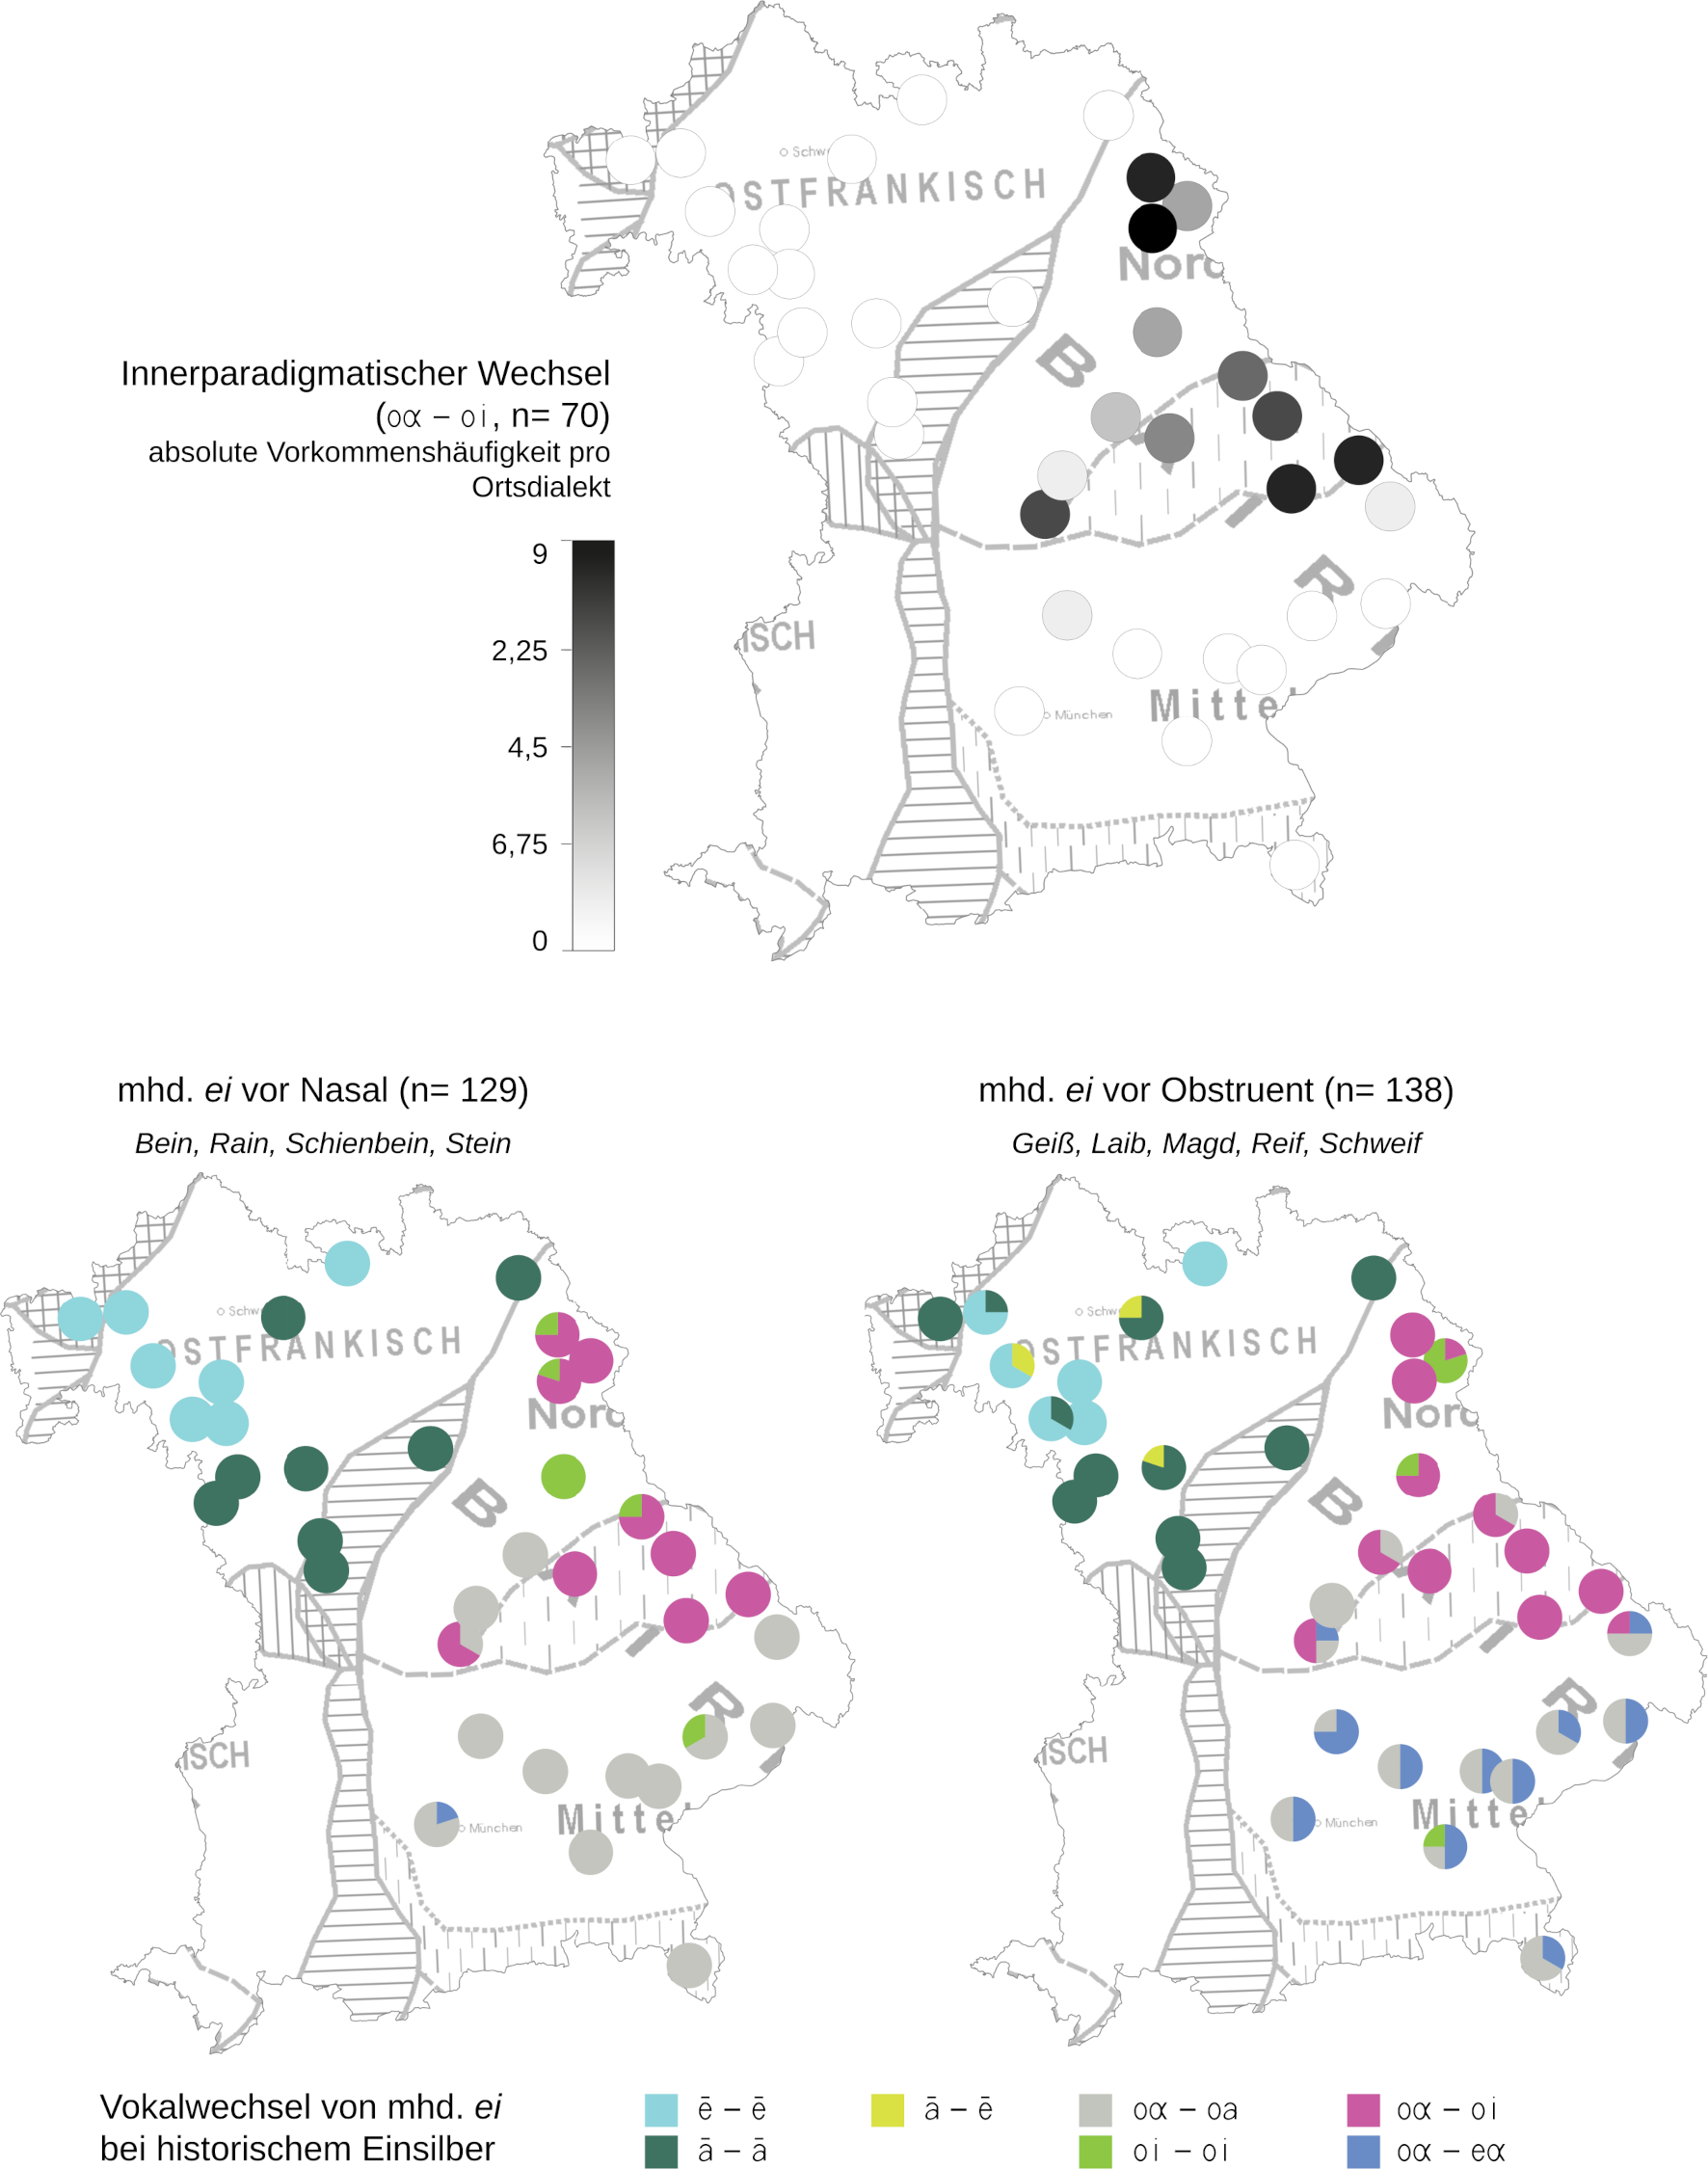
\includegraphics[width=\textwidth]{figures/Karte5.png}
\caption{Häufigkeitsverteilung der Vokalwechsel von mhd. \textit{ei} bei historischen Einsilbern und Chloroplethkarte mit absoluter Vorkommenshäufigkeit des \textit{oα-oi}{}-Wechsels}
\label{map:5}
\end{map}

Dieser innerparadigmatische Wechsel findet sich in Flexionsformen und Wortbildungen, z.\,B. Sg. \teuthoo{lo<.A}{lôͅα} -- Pl. \teuthoo{lo<i}{lôi} -- Dim. \teuthoo{lo.<iw@l@}{lôͅiw̥l̥} (‚Laib‘, nordbair.-mittelbair. Grafenkirchen). „Umlautähnlich“ ist der Kontrast der Vokalqualität nach \citet[66]{Rowley1997} deshalb, weil der Vokalwechsel zwar dem Umlaut ähnelt, aber keine Korrelation der Zungenhöhe besteht (vgl. \sectref{sec:7.1.2.1.1}). Im UG gibt es neben diesem Wechsel ohne Korrelation der Zungenhöhe Belege für einen Diphthongwechsel mit Zungenhöhenkorrelation, d.\,h. einen analogen Umlaut \teuthoo{oA}{oα} -- \teuthoo{eA}{eα} anstelle des lauthistorischen Diphthongs \teuthoo{oi}{oi}. Im nördlichen Nordbair. ist dieser Diphthongwechsel v.\,a. in Komparativformen belegt, \citet[66]{Rowley1997} führt die Komparativform \teuthoo{weac!a}{weaꭖa} ‚weicher‘ neben der lautgesetzlichen Realisierung \teuthoo{woic!a}{woiꭖa} an.\footnote{Vgl. auch \citet[§75.1]{Kollmer1987}, \citet[§75c6]{Micko1930}, \citet[96]{Roth1940}, \citet[§56.4]{Schießl1914}. Im mittelbair. Dialekt der Hallertau ist der analoge Umlaut in Komparativformen „keineswegs obligatorisch“, \textit{wɔ\textsuperscript{a}}\textit{ha} ist neben \textit{wɛ\textsuperscript{a}}\textit{ha} ‚weicher‘ belegt \citep[167]{Zehetner1978}. \citet[168]{Zehetner1978} bietet daneben Belege für den analogen Umlaut in Wortbildungen, z.\,B. /brɛ\textsuperscript{a}dn/ ‚Breite‘ zu /brɔ\textsuperscript{a}d/ ‚breit‘, /sɔ\textsuperscript{a}h/ ‚Urin‘ und /sɛ\textsuperscript{a}hin/ ‚nach Urin riechen‘, aber /gɔ\textsuperscript{a}s/ ‚Geiß‘, /gɔ\textsuperscript{a}sln/ ‚nach Geiß riechen‘.}  In den BSA-Daten findet sich der analoge Umlaut mit Zungenhöhenkorrelation (\teuthoo{eA}{eα}) vor allem in den mittelbair. Ortsdialekten bei den Lexemen \textit{Schweif}, z.\,T. \textit{Reif} und \textit{Geiß}. Der einzige Beleg des Wechsels \teuthoo{oA}{oα} -- \teuthoo{eA}{eα} vor Nasal in \textit{Stein} im mittelbair. Pasing (\teuthoo{s\#de<A<nA}{šdêα̂nα} neben \teuthoo{s\#do>+A+}{šdỗα̃}, \teuthoo{s\#do>+A+nA}{šdỗα̃nα}) ist nach \citet[168]{Zehetner1978} „nicht eigentlich ländlich, sondern anscheinend münchnerischer Provenienz“ (vgl. \citealt[Karte 78]{SOB4}). Im Dialekt von München und im westmittelbair. Eisenhofen ist dieses analoge Umlautmuster auch bei mhd. \textit{î} in \textit{Streifen} (mhd. \textit{strîfe}) belegt: \teuthoo{s\#dro.2Af}{šdrōͅαf} -- \teuthoo{s\#tre.Af}{štreͅαf} (\citealt[79]{Wittmann1943}, vgl. \citealt[44]{White1966}).\footnote{Im Dialekt von Eisenhofen ist das Umlautmuster \teuthoo{oA}{oα} -- \teuthoo{eA}{eα} bei Maskulina und Neutra stark besetzt, da es -- nach \citet[44]{White1966} -- die rezente Entsprechung von mhd. \textit{ô}/\textit{œ} (\teuthoo{flo.ax}{f‌loͅax} -- \teuthoo{fle.ax}{f‌leͅax} ‚Floh‘) und von mhd. \textit{o}/\textit{ö} vor /r/ (\teuthoo{kho.a«r»b}{khoͅa(r)b} -- \teuthoo{khe.a«r»b}{kheͅa(r)b} ‚Korb‘) bildet. Der analoge Umlaut bei mhd. \textit{ei} in \textit{Streifen} und \textit{Schweif} entspricht diesem Muster. Neben Belegen eines analogen Umlauts \teuthoo{oA}{oα} -- \teuthoo{eA}{eα} in Plural- und Komparativformen (\teuthoo{s\#wo.2Af}{šwōͅαf} -- \teuthoo{s\#weAff}{šweαff} ‚Schweif‘, \teuthoo{bro.Ad}{broͅαd} -- \teuthoo{bre2AdA}{brēαdα} ‚breit‘) berichtet \citet[85]{Grundler1951} für das mittelbair. Erding außerdem von semantischen Unterschieden bei Formen ohne bzw. mit analogem Umlaut: \teuthoo{bro2.Adn}{brōͅαdn} ‚breiter Acker‘, \teuthoo{bre2Adn}{brēαdn} ‚Breite (Maßbezeichnung)‘ für mhd. \textit{breite}.}

Die Entsprechung von mhd. \textit{ei} ist im Verbreitungsgebiet vor Nasal z.\,T. anders verlaufen als vor Obstruent, weshalb die beiden lautlichen Umgebungen in \mapref{map:5} getrennt behandelt wurden (vgl. \citealt[Karten 20--22]{Gütter1971}, \citealt[56--59]{RennKönig2006}, \citealt[66 und Karte 12]{Rowley1997}). An der Raumbildung der Karte lässt sich dabei die unterschiedliche Normalentwicklung im Ofr. und im Bair. nachvollziehen. In den ofr. Ortsdialekten finden sich die monophthongischen Realisierungen \teuthoo{e2}{ē} oder \teuthoo{a2}{ạ̄}, während mhd. \textit{ei} in den bair. Dialekten diphthongisch realisiert wird. Interessant an den ofr. Daten ist, dass es auch hier Belege für einen analogen Umlaut gibt (einzig bei dem Lexem \textit{Reif}, Typ \teuthoo{ra2v}{rāv} -- \teuthoo{re2v}{rēv}).\footnote{In Erlabrunn gibt es zudem einen Einzelbeleg für eine Alternation der Vokalqualität mittels Entrundung des Stammvokals bei gleichzeitiger Kürzung: \teuthoo{ro"?:v5}{rȫ{\doubleogonek}v̩} -- \teuthoo{re?v5}{rëv̩} (‚Reif‘).}

Im bair. Teil des UGs gibt es eine Zweiteilung. Im Nordbair. und im nordbair.-mittelbair. Übergangsgebiet überwiegt die innerparadigmatische Alternation \teuthoo{oA}{oα} -- \teuthoo{oi}{oi}, während im größten Teil der mittelbair. Tiefenbohrungspunkte die Realisierung von mhd. \textit{ei} ohne innerparadigmatischen Wechsel überwiegt (\teuthoo{oA}{oα} -- \teuthoo{oA}{oα}). Der Diphthong \teuthoo{oA}{oα} entspricht hier der mittelbair. Normalentwicklung von mhd. \textit{ei} (vgl. \citealt[§20h]{Kranzmayer1956}). Auch im Nordbair. sowie im nordbair.-mittelbair. Übergangsgebiet gibt es Belege für Formen ohne innerparadigmatischen Wechsel, jedoch ist dieser innerparadigmatische Ausgleich lexemweise zu \teuthoo{oi}{oi} erfolgt, im gesamten UG etwa bei \textit{Rain} (vgl. \citealt[441]{Götz1987}, \citealt[§75]{Micko1930}). Bemerkenswert ist, dass die Ausdifferenzierung der rezenten Entsprechungen von mhd. \textit{ei} relativ jung zu sein scheint. \citet[§14]{Micko-Repp1933} gibt den lautgesetzlichen \teuthoo{oA}{oα}-\teuthoo{oi}{oi}-Wechsel als Variante der älteren Generation an, die im mittelbair. Wadetstift neben Formen ohne innerparadigmatischen Wechsel (\teuthoo{oi}{oi} -- \teuthoo{oi}{oi}) belegt ist; der Wechsel \teuthoo{oA}{oα} -- \teuthoo{eA}{eα} sei als „jüngste Erscheinung“ im Basisdialekt noch selten.


\begin{map}
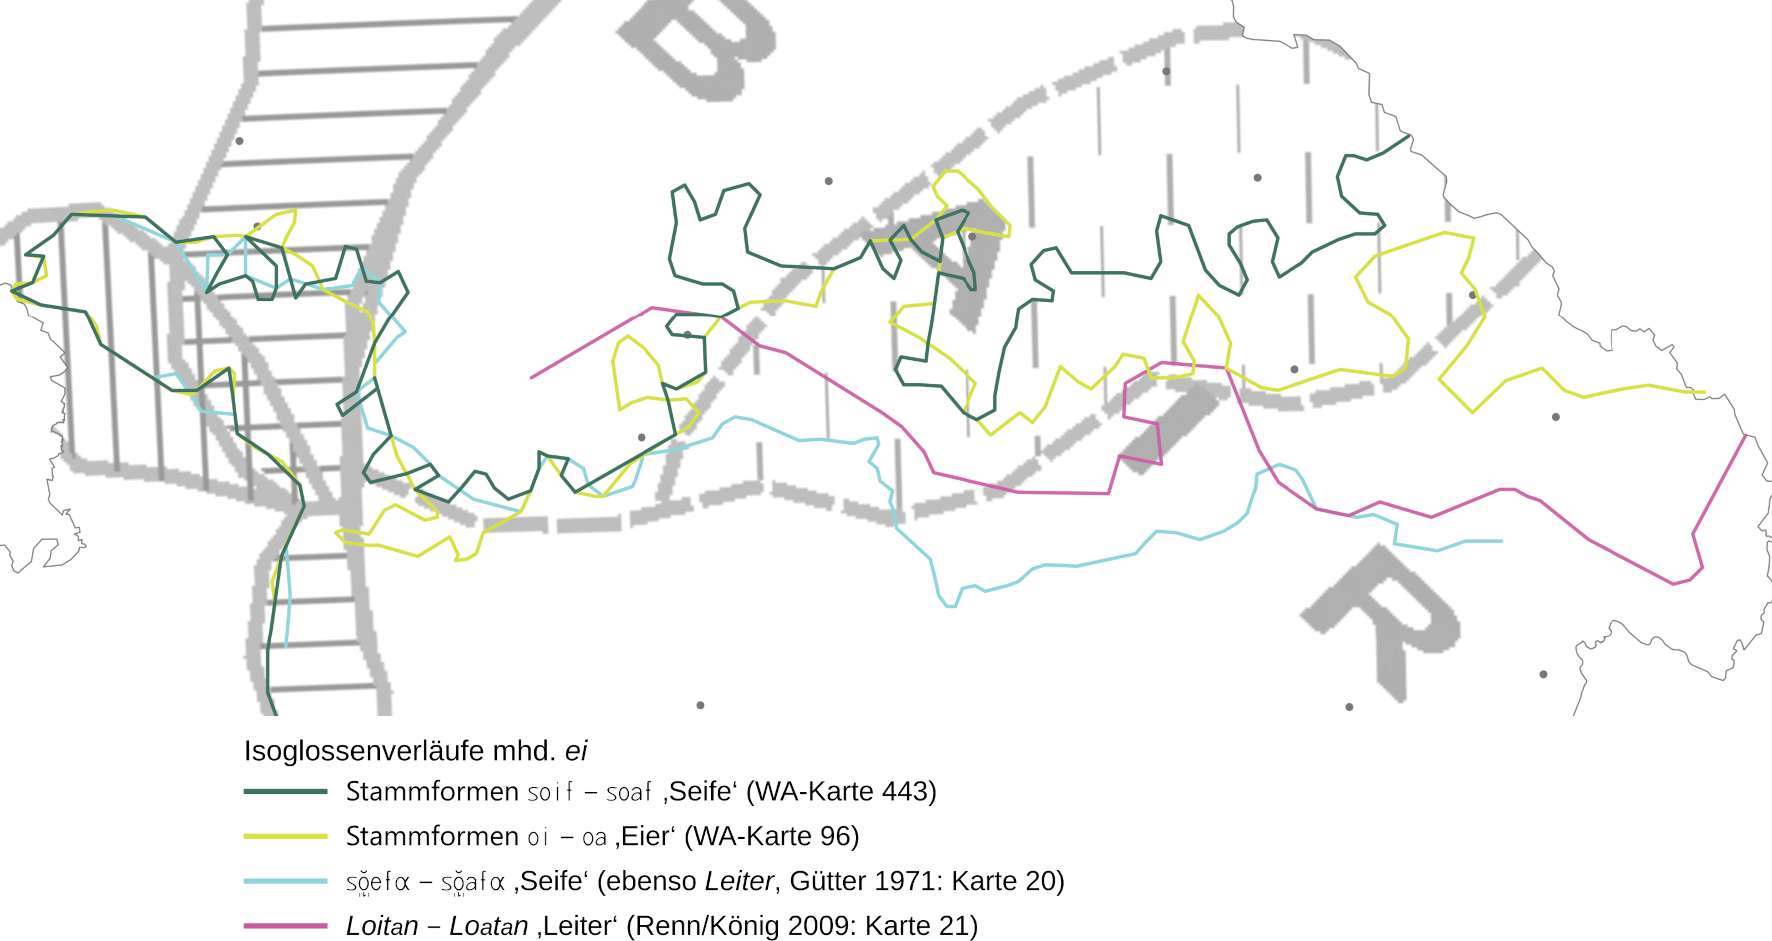
\includegraphics[width=\textwidth]{figures/Karte6.png}
\caption{Lexemspezifische Isoglossenverläufe von mhd. \textit{ei} im nordbairisch-mittelbairischen Übergangsgebiet}
\label{map:6}
\end{map}

Ein Vergleich mit den relevanten Wenker-Karten\footnote{Im \textit{Sprachatlas des Deutschen Reich} sind drei Lexeme mit historischen Mehrsilbern kartiert (\textit{Eier}, \textit{Kleider}, \textit{Seife}). Die \citealt{WA}-Karte \textit{Kleider} (Akk.Pl.) ist dabei nur bedingt aufschlussreich, da im größten Teil des Bair. das Heteronym \textit{Gewand} verbreitet ist.} zeigt, dass auch im südlichen Nordbair., d.\,h. in jenem Areal, für das die Leitform \teuthoo{oi}{oi} gilt, Formen mit dem Diphthong \teuthoo{oA}{oα} in der Stammform (\textit{kload}{}-, \textit{soaf}{}-)\footnote{\citealt{WA}-Karte 444 (\textit{Seife}, Akk.Sg.fem.) zeigt, dass \textit{Seife} in diesem Gebiet auch synchron zweisilbig in der \textit{n}{}-erweiterten Form (und nicht etwa in der einsilbigen apokopierten Form) realisiert wird.} belegt sind. Damit ist auch im Wenker-Material eine Varianz zwischen Vokalwechsel und innerparadigmatischem Ausgleich (nach mittelbair. Normalentwicklung) zu finden. Gleichzeitig zeigen die Isoglossenverläufe, dass die Realisierung des Diphthongs in diesem Übergangsgebiet lexemspezifisch zu sein scheint (\mapref{map:6}).

Aufgrund der geringen Anzahl der abgefragten Lexeme für die jeweilige phonologische Umgebung von mhd. \textit{ei} vor Nasal vs. Obstruent ist es schwierig, über lexemspezifische Entwicklungen hinaus zu generalisieren. Die areale Verteilung der Diphthongwechsel ergibt in der Tendenz für die nordbair. Ortsdialekte die umlautähnlichen Wechsel \teuthoo{oA}{oα} -- \teuthoo{oi}{oi} sowie den Typus \teuthoo{oi}{oi} -- \teuthoo{oi}{oi} ohne Alternanz, während in den mittelbair. Orten der Typus \teuthoo{oA}{oα} -- \teuthoo{oA}{oα} (sowie vereinzelt \teuthoo{oi}{oi} -- \teuthoo{oi}{oi}) und die Alternation mit Zungenhöhenkorrelation \teuthoo{oA}{oα} -- \teuthoo{eA}{eα} belegt ist. Im nordbair.-mittelbair. Übergangsgebiet sind neben dem \teuthoo{oA}{oα}-\teuthoo{oi}{oi}-Wechsel beide Ausgleichsvarianten (\teuthoo{oA}{oα} -- \teuthoo{oA}{oα} und \teuthoo{oi}{oi} -- \teuthoo{oi}{oi}) zu finden. Damit sind die innerparadigmatischen Diphthongwechsel ein spezifisches Phänomen des Nordbair. und des nordbair.-mittelbair. Übergangsgebiets, während der analoge Umlaut \teuthoo{oA}{oα} -- \teuthoo{eA}{eα} im Mittelbair. gilt, sich aber nach Norden hin auszudehnen scheint. Laut \citet[167]{Zehetner1978} finden sich diese \teuthoo{oA}{oα}-\teuthoo{eA}{eα}-Formen in der mittelbair. Hallertau, nicht aber in dem Gebiet nördlich bis zur Donau („Donauland“), da man dort der Markierung der Pluralinformation durch analogen Umlaut aufgrund der lautgesetzlichen \teuthoo{oA}{oα}-\teuthoo{oi}{oi}-Alternation nicht „bedurfte“. Während sich in den vorliegenden Daten ein einzelner Beleg der \teuthoo{oA}{oα}-\teuthoo{eA}{eα}-Alternation im südlichen Nordbair. in Oberdolling (\teuthoo{ro4Af}{rọαf} -- \teuthoo{re.Af,}{reͅαf͓} ‚Reif‘) findet, zeigen die BSA-Karten zur Pluralmarkierung von \textit{Geiß} demgegenüber ein relativ geschlossenes Gebiet des Typs \teuthoo{go<As}{ɡôαs} -- \teuthoo{geAS}{ɡeᾳʃ}, das die Hallertau und auch das „Donauland“ nördlich davon umfasst (vgl. \citealt[Karte 8]{SOB4}, \citealt[Karte 89/90]{SNiB7}).\largerpage

Insgesamt scheint die Realisierung von mhd. \textit{ei} mit oder ohne Vokalwechsel in den untersuchten Ortsdialekten aber stark lexemspezifisch zu sein. Aus flexionsmorphologischer Perspektive führen beide Realisierungsvarianten des innerparadigmatischen Vokalwechsel (\teuthoo{oA}{oα} -- \teuthoo{oi}{oi} bzw. \teuthoo{oA}{oα} -- \teuthoo{eA}{eα}) zu differenten Singular- und Pluralformen. In den Singular- und Pluralformen ohne innerparadigmatische Alternation wird der Plural nicht modulativ in Form eines (umlautähnlichen oder analogen Umlaut-)Vokalwechsels, sondern mittels anderer Pluralmarkierungsstrategien respektive Nullplural gebildet. \citet{Wildfeuer2001} beschreibt in seiner Apparent-time-Studie dreier mittelbair. Sprechergruppen einen Wandel hin zu einer kumulativen Markierung des Plurals von \textit{Stein}. In der älteren Sprechergruppe ist der Diphthongwechsel von mhd. \textit{ei} im Sg. [õα] zu Pl. [ãi] mit 80\,\% belegt, bei der mittleren Sprechergruppe mit 70\,\%, während die jüngere Gruppe den Plural von \textit{Stein} nur zu 30\,\% rein modulativ mit Diphthongwechsel bildet und in der Mehrzahl (70\,\%) die „Maximalmarkierung“, d.\,h. den modulativ-additiven Plural des Typs \textit{šdõα} -- \textit{šdãinα}, verwendet \citep[188]{Wildfeuer2001}.

Als Pluralmarkierungsverfahren funktionalisiert und produktiv ist der Diph\-thong\-wech\-sel \teuthoo{oA}{oα} -- \teuthoo{oi}{oi} da, wo er unabhängig von der phonologischen Umgebung der historischen Ein- vs. Mehrsilbigkeit in (ehemals) zweisilbigen Substantiven erscheint (vgl. \tabref{tab:21}): \teuthoo{gmo+A}{ɡmõα} -- \teuthoo{gmoi}{ɡmoi} ‚Gemeinde‘ (nordbair.-mittelbair. Bernhardswald), \teuthoo{so4<AfA}{sộαfα} -- \teuthoo{so4<e4f,An}{sộẹf͓αn} ‚Seife‘ (nordbair. Riedenburg), \teuthoo{s\#po<AH}{špôαhͯ} -- \teuthoo{s\#po<EHAn}{špôəhͯαn} ‚Speiche‘ (mittelbair. Wolfersdorf), \teuthoo{o<AHA}{ôαhͯα} -- \teuthoo{o4<eXAn}{ộeꭗαn} ‚Eiche‘ (nordbair. Oberdolling).

\begin{table}
\begin{tabularx}{\textwidth}{QQ}
\lsptoprule
Historische Einsilber & Historische Mehrsilber\\
\midrule
\textit{Bein, Ei}, \textit{Geiß}, \textit{Laib}, \textit{Magd/Maid,}\footnote{Mhd. \textit{ege} in \textit{megetlîn} wird zu \textit{ei} kontrahiert (ebenso in \textit{getregede} ‚Getreide‘), kontrahiertes \textit{ei} entwickelt sich in der Folge in den untersuchten Dialekten analog zu mhd. \textit{ei}, z.\,B. \teuthoo{mo.2i\textsuperscript{d}l@}{mōͅi\textsuperscript{d}l̥}, \teuthoo{d5ro2.i}{d̩rōͅi} im nordbair. Kallmünz \citep[441]{Götz1987} vs. \textit{drɔ\textsuperscript{a}}\textit{d} in der mittelbair. Hallertau (\citealt[158]{Zehetner1978}, vgl. \citealt[32]{Förster1912/13}, \citealt[§81]{Gebhardt1907}, \citealt[83]{Grundler1951}, \citealt[§75d]{Micko1930}.} \textit{Rain, Reif(en)}, \textit{Schweif}, \textit{Seil}, \textit{Stein}  & \textit{Breite}\footnote{nur SMF} \textit{Eiche}, (\textit{Ge}{}-)\textit{Leise}, \textit{Gemeinde}, \textit{Seife}, \textit{Speiche}\\
\lspbottomrule
\end{tabularx}
\caption{Lexeme mit mhd. \textit{ei} als Stammvokal im Korpus}
\label{tab:21}
\end{table}


\subsubsubsection{Wechsel der Zungenhöhe}\label{sec:7.1.2.1.3}\largerpage[2]
Im UG sind mhd. \textit{e} und \textit{ö} in Dehnung teilweise zu \textit{ī} gehoben worden, im östlichen Ofr. und im nördlichen Nordbair. werden sie diphthongisch als \teuthoo{I2A}{ı̄α} realisiert (vgl. \sectref{sec:7.1.2.1.1}).{\interfootnotelinepenalty=10000\footnote{Vgl. \citet[Karte 3]{Gütter1971}, \citet[4d]{Kranzmayer1956}, \citet[73--74 und Karte 15]{Rowley1997}, \citet[121--125 und Karte 22]{Steger1968}, \citealt[75]{SMF3}, \citet[1110]{Wiesinger1983c}. Daneben wurde in der Parallelreihe mhd. \textit{e-ö-o} auch mhd. \textit{o} zu \textit{ū} gehoben (vgl. \citealt[Karte 4]{Gütter1971}, \citealt[73 und Karte 15]{Rowley1997}).}} Die Dehnung des Stammvokals ist im Rahmen der Einsilberdehnung nur in der Singularform, nicht aber in der additiven und damit zweisilbigen Pluralform eingetreten, weshalb in jenen Ortsdialekten, in denen mhd. \textit{e} und \textit{ö} in Dehnung gehoben wurden, innerparadigmatische Alternationen zwischen gehobenem Vokal in der Singularform und im Plural mhd. \textit{e} bzw. \textit{ö} in Normalentwicklung erscheinen (mhd. \textit{ö} nur in einer Form mit sogenannter Markiertheitsumkehrung im ofr.-hess Wiesthal, vgl. \tabref{tab:22}).
Die Alternation besteht damit in einem lautgesetzlich entstandenen Wechsel der Zungenhöhe bei zwei Palatalvokalen. Bemerkenswert sind hier die Belege für \textit{Erle} und \textit{Kerze} im Nord- und Mittelbair., da der Wechsel der Zungenhöhe nicht bei historischen Ein-, sondern Zweisilbern erscheint und damit nicht lautgesetzlich ist.

Daneben gibt es eine weitere Form eines Wechsels der Zungenhöhe zwischen geschlossenem \teuthoo{e24}{ẹ̄} und offenem \teuthoo{e.}{eͅ}, den \citet[116--117]{Rowley1997} für das nördliche Nordbair. anführt und der sich in den vorliegenden Daten im nordbair. Windischeschenbach und Nabburg und daneben im ofr.-nordbair. Übergangsgebiet (Tiefenbohrungspunkte Pfofeld\footnote{Karten 25/26 (mhd. \textit{e} in \textit{Zähne}, \textit{Blätter}) und 28 (mhd. \textit{ö} in \textit{Vögel}) in \citet{Kollmann1961} zeigen die Isoglossenverläufe der Hebung von mhd. \textit{e}, \textit{ö} in Dehnung im ofr.-nordbair. Übergangsgebiet und dass diese im Tiefenbohrungspunkt Pfofeld ebenfalls teilweise erfolgt ist, vgl. die Formen in den eigenen Daten: \teuthoo{vu42gJ}{vụ̄ɡ{\lkreis}} -- \teuthoo{vi4"gJ}{vị̄ɡ{\lkreis}} -- \teuthoo{ve.hAl.A}{veͅhαlͅα} ‚Vogel‘, aber \teuthoo{dsu42}{dsụ̄} -- \teuthoo{dse42}{dsẹ̄} ‚Zahn‘ (vgl. \citealt[22--24]{Kollmann1961} sowie \citealt[Karte 33/34]{Brendel1962}, \citealt[§12 und Karte 3]{Kaußler1962}, \citealt[Karte 22]{Kopp1959}).} und Kirchensittenbach) findet (vgl. \citealt[§65]{Kollmer1985}).

Ortsdialektspezifisch ist daneben die Senkung von mhd. \textit{i} in historischen Zweisilbern und die resultierende innerparadigmatische Alternation in Wiesthal im ofr.-hess. Übergangsgebiet (vgl. \citealt[1108]{Wiesinger1983c}).

\begin{table}
\small
\begin{tabularx}{\textwidth}{llllQ}
\lsptoprule
& {Singular} & {Plural} & &\\
\midrule
\makecell[tl]{{mhd. \textit{ë},}\\
{mhd. \textit{e}}} & \teuthoo{brI9."d}{brı\klammeruntenpost{}̄ͅd} & \teuthoo{bre4dE}{brẹdə} & \multicolumn{2}{>{\raggedright\arraybackslash}p{.53\textwidth}}{‚Brett‘ (ofr. Burgbernheim, daneben ofr.-nordbair. Pfofeld)}\\
\tablevspace
& \teuthoo{vôe?e\$d}{v{\aufstrih}ëe̤d} & \teuthoo{v\%ôe?i.dA}{v͈{\aufstrih}ëiͅdα} & \multicolumn{2}{>{\raggedright\arraybackslash}p{.53\textwidth}}{‚Feld‘ (nordbair. Oberdolling, daneben ofr.-nordbair. Kirchensittenbach)}\\
\tablevspace
& \teuthoo{ni94"s\#d}{ni\klammeruntenpost{}̣̄šd} & \teuthoo{ne.s\#dA}{neͅšdα} & \multicolumn{2}{>{\raggedright\arraybackslash}p{.53\textwidth}}{‚Nest‘ (ofr.-nordbair. Mitteleschenbach, daneben ofr. Burgbernheim und Pfofeld, nordbair. Groschlattengrün, Tirschenreuth und Windischeschenbach, vgl. \citealt[Karte 40]{SUF3})}\\
\tablevspace
& \teuthoo{vle42g}{vlẹ̄ɡ} & \teuthoo{vle.gá\_}{vleͅɡ͈ʰ} & \multicolumn{2}{>{\raggedright\arraybackslash}p{.53\textwidth}}{‚Fleck‘ (ofr.-nordbair. Pfofeld, vgl. \citealt[69]{SNOB1})}\\
\tablevspace
& \teuthoo{gðNec1d}{ɡ̩ŋeX\⚬d} & \teuthoo{gNe.c1t}{ɡŋeͅX\⚬t} & \multicolumn{2}{>{\raggedright\arraybackslash}p{.53\textwidth}}{‚Knecht‘ (nordbair. Nabburg, daneben ofr.-nordbair. Pfofeld, nordbair. Windischeschenbach)} \\
\tablevspace
& \teuthoo{i.“A2l}{īͅᾱl} & \teuthoo{e\$Aln}{e̤αln} & \multicolumn{2}{>{\raggedright\arraybackslash}p{.53\textwidth}}{‚Erle‘ (mittelbair. Neukirchen am Inn, daneben mittelbair. Waldhof)}\\
\tablevspace
& \teuthoo{g\_iEtSn@}{ɡʰiətʃn̥} & \teuthoo{g\_e.EtSn@}{ɡʰeͅətʃn̥} & \multicolumn{2}{>{\raggedright\arraybackslash}p{.53\textwidth}}{‚Kerze‘ (nordbair. Groschlattengrün, daneben mittelbair. Inning am Holz und Neukirchen am Inn)}\\
\tablevspace
{mhd. \textit{i}} & \teuthoo{vi“s\#}{vīš} & \teuthoo{ve94s\#}{ve\klammeruntenpost{}̣̄š} & {‚Fisch‘} & \multirow[t]{4}{=}{(ofr.-hess.-Wiesthal, vgl. \citealt[Karte 4]{SUF1}, \citealt{WA}-Karte 449 ‚Tische‘)}\\
& \teuthoo{gri“v5}{ɡrīv̩} & \teuthoo{gre4v5}{ɡrẹv̩} & {‚Griff‘} & \\
& \teuthoo{s\#di“c}{šdīX} & \teuthoo{s\#deX}{šdeꭗ} & {‚Stich‘} & \\
& \teuthoo{di“s\#}{dīš} & \teuthoo{dswe2}{dswē} \teuthoo{des#}{deš} & {‚Tisch‘} & \\
& \teuthoo{wi“E.d}{wīəͅd} & \teuthoo{we4d5\_}{wẹd̩ʰ} & \multicolumn{2}{>{\raggedright\arraybackslash}p{.53\textwidth}}{‚Wirt‘ (ofr. Erlabrunn, daneben ofr. Ochsenfurt, vgl. \citealt[Karte 16]{SUF1})}\\
\tablevspace
{mhd. \textit{ö}} & \makecell[tl]{\teuthoo{dsi.“bv5}{dsīͅbv̩}\\(neben\\\teuthoo{dse\$2bv}{dsē̤bv})} & \makecell[tl](\teuthoo{di la.NE dse4bv5}{di laͅŋə dsẹbv̩}) & \multicolumn{2}{>{\raggedright\arraybackslash}p{.53\textwidth}}{‚Zopf‘ (ofr.-hess.-Wiesthal)}\\
\lspbottomrule
\end{tabularx}
\caption{Belege von innerparadigmatischem Wechsel der Zungenhöhe im UG ($n=26$)}
\label{tab:22}
\end{table}

\subsubsection{Kontraste der Vokalquantität}
\label{sec:7.1.2.2}
Innerparadigmatische Kontraste der Quantität des Stammvokals können als Numerusmarker funktionalisiert sein. Die Pluralmarkierung findet dabei (wie auch die Modulation der Vokalqualität) an einer „symbolverdächtigen Stelle des Wortes“ \citep[283]{Harnisch1994a} statt (anders als beispielsweise Konsonantenelisionen oder -fortisierungen im Stammauslaut, vgl. \sectref{sec:7.1.2.3}). Kürzungen der Vokalquantität werden hier nicht als Form eines subtraktiven Plurals, sondern als Modulationen der Vokalquantität klassifiziert (vgl. \citealt[25]{Birkenes2014}, \citealt[584]{Dressler2000}, anders \citealt{Nübling2006} für das Luxemburgische).

Im UG erfolgte phonologischer Wandel der Vokalquantität durch Dehnung in offener Tonsilbe, durch Dehnung von mhd. Einsilbern mit betontem Kurzvokal sowie durch Kürzung historischer Dreisilber.\footnote{Siehe hierzu \citet[§E33 und §34k]{Kranzmayer1956}, \citet[69--73]{Rowley1997}, \citet[181--189]{Schirmunski1962}, \citet{Seiler2009}, \citet[35--41]{Steger1968}, \citet[1091--1094]{Wiesinger1983a}.} Laut \citet[§34k.1]{Kranzmayer1956} entspringen sämtliche historische Veränderungen der Vokalquantität im UG dem „Bemühen, die Wortkörper unabhängig von ihrer Silbenzahl gleich lang zu gestalten“ (vgl. \citealt[12]{Kollmer1949}). Einen ähnlichen Erklärungsansatz der Quantitätsverhältnisse im Ofr. und Bair. bietet die Morentheorie (vgl. einführend \citealt[1071--1074]{Auer1989} sowie \citealt{Auer1991}): Das minimale Wort besteht in Dialekten, die Einsilberdehnung durchgeführt haben, aus einer zweimorigen Silbenstruktur (vgl. \citealt[254--260]{Seiler2009} sowie \sectref{sec:7.1.2.3.1}). Um diese zu erfüllen, wird der kurze (einmorige) Vokal zu einem langen (zweimorigen) Vokal gedehnt, der auslautende Konsonant ist nicht-morenwertig.

Werden historische Einsilber synchron mit Kurzvokal realisiert, so kann dies laut \citet[70]{Rowley1997} das Ergebnis von standardsprachlichem Einfluss oder von innerparadigmatischem Ausgleich sein, \citet[132--133]{Schübel1955} führt für den ofr. Dialekt Stadtsteinachs zudem die auf den Stammvokal folgende Konsonantenverbindung sowie die Gebrauchsfrequenz als mögliche Einflussfaktoren an. \citet[§34k5]{Kranzmayer1956} zufolge ist die Einsilberdehnung im Nordbair. und Ofr. „am besten bewahrt“, doch sind die lautgesetzlichen Quantitätsverhältnisse im Ofr. laut \citet[71]{Rowley1997} durch innerparadigmatischen Ausgleich „mancherorts stark verwischt“ (vgl. \citealt[70--71]{Heilig1898}, \citealt[1]{Heinebrodt1963}, \citealt[Karte 22]{Kranzmayer1956}). Erhalten sind die Quantitätskontraste in einem Teil des Ofr. (Bayreuther, Bamberger und Erlanger Raum) dagegen systematisch in Kombination mit Kontrasten der Vokalqualität, etwa bei einem Wechsel der Zungenhöhe wie in \teuthoo{vle2g}{vlēg} -- \teuthoo{vle.g}{vleͅɡ} ‚Fleck‘ \citep[194]{Rowley1997}.

Aus flexionsmorphologischer Perspektive sind die phonologischen Prozesse, die die Vokalquantität betreffen, dann relevant, wenn innerparadigmatische Alternationen zwischen Kurz- und Langvokal entstehen, wie es infolge der Einsilberdehnung der Fall ist. Der Stammvokal der einsilbigen Singularform wurde gedehnt, der Stammvokal in geschlossener Tonsilbe der zweisilbigen (additiven) Pluralform und der Diminutivform blieben kurz, z.\,B. \teuthoo{blo942d\_}{blo\klammeruntenpost{}̣̄dʰ} -- \teuthoo{ble):dA}{ble\klammeruntenpost{}{\doubleogonek}dα} ‚Blatt‘ (ofr.-nordbair. Mitteleschenbach), \teuthoo{vo2s5}{vōs̩} -- \teuthoo{ve.s4Er}{veͅṣər} -- Dim. \teuthoo{ve.sla}{veͅsla} ‚Fass‘ (ofr. Hallerstein).\footnote{Quantitätskontraste durch Einsilberdehnung und erhaltene Kürze aufgrund von Mehrsilbigkeit erscheint -- wie die Diminutivformen zeigen -- nicht nur innerhalb von Flexionsparadigmen, sondern auch bei Wortbildungen, wie die ofr. Beispiele von \citet[132]{Schübel1955} illustrieren: \teuthoo{wI2Ed}{wı̄əd} -- \teuthoo{wedA}{wedα} -- \teuthoo{wedshaus}{wedshaus} ‚Wirt -- Wirtin -- Wirtshaus‘, \teuthoo{gnu2ofb}{ɡnūofb} -- \teuthoo{gnobflox}{ɡnobf‌lox} -- \teuthoo{gno?bflA}{ɡnöbf‌lα} ‚Knopf -- Knopfloch -- Knöpfchen‘.}  Wies die zweisilbige Pluralform eine offene Tonsilbe auf, trat lautgesetzliche Dehnung in offener Tonsilbe ein, z.\,B. \teuthoo{ro.2d5\_}{rōͅd̩ʰ} -- \teuthoo{re9.2dE.}{re\klammeruntenpost{}̄ͅdəͅ} -- Dim. \teuthoo{re.2dJA94.}{rēͅd{\lkreis}α\klammeruntenpost{}̣ͅ} ‚Rad‘ (ofr. Burgbernheim), \teuthoo{glo.2s}{ɡlōͅs} -- \teuthoo{gle.2sA}{ɡlēͅsα} -- Dim. \teuthoo{gla42sl}{ɡlạ̄sl} ‚Glas‘ (mittelbair. Kirchensur). Bei mhd. Substantiven mit Schwa als Pluralmarker entstanden infolge eines zweiten (nachfolgenden)\footnote{Hierzu führt \citet[§266]{Heilig1898} aus (vgl. \citealt[48]{Roth1940}): „Diese Formen [d.\,h. Formen mit innerparadigmatischem Quantitätenkontrast des Typs vīš -- viš ‚Fisch‘, GN] beweisen, daß nach dem Abfall des \textit{e} die Dehnung der einsilbigen Wörter bereits abgeschlossen gewesen sein muss.“}  phonologischen Prozesses, der Apokope, rein stammaffizierende Flexionsformen des Typs \teuthoo{vi“s\#}{vīš} -- \teuthoo{vI3s\#5}{vı̆š̩} ‚Fisch‘ (nordbair. Groschlattengrün). Die phonologische Umgebung der Einsilberdehnung (bestehend im Kontrast zur zweisilbigen Pluralform) war nicht mehr transparent (vgl. \citealt[188]{Seiler2008}).

\begin{table}
\small
\begin{tabularx}{\textwidth}{lQQQ>{\raggedright\arraybackslash}p{.1\textwidth}>{\raggedright\arraybackslash}p{.25\textwidth}}
\lsptoprule
\makecell[tl]{{Quantitäts-}\\{muster}} & {Singular} & {Plural} & {Diminutiv} & &\\
\midrule
{(a) K -- K} -- K & \teuthoo{dê}{d{\burgereshwa}} \teuthoo{qågê}{ʔ{\burgeroalpha}ɡ{\burgereshwa}} & \teuthoo{di}{di} \teuthoo{qa94gê}{ʔa\klammeruntenpost{}̣ɡ{\burgereshwa}} & \teuthoo{Aq}{αʔ} \teuthoo{a94gêlA}{a\klammeruntenpost{}̣ɡ{\burgereshwa}lα} & \multicolumn{2}{>{\raggedright\arraybackslash}p{.35\textwidth}}{‚Acker‘ (ofr. Ahorn)}\\
 &   \teuthoo{do4xd}{dọxd} & \teuthoo{de?cd}{dëXd} & \teuthoo{de?cdlA}{dëXdlα} & \multicolumn{2}{>{\raggedright\arraybackslash}p{.35\textwidth}}{‚Docht‘ (ofr. Hüttenheim)}\\
 \tablevspace
 {(b) L -- L} -- L & \teuthoo{go.2wl@}{ɡōͅwl̥} & \teuthoo{go.2wl@}{ɡōͅwl̥} & \teuthoo{go"?.wElE}{ɡȫͅwələ} & \multicolumn{2}{>{\raggedright\arraybackslash}p{.3\textwidth}}{‚Gabel‘ (ofr. Gemünden am Main)}\\
 &  \teuthoo{glo.2s}{ɡlōͅs} & \teuthoo{gle.2sA}{ɡlēͅsα} & \teuthoo{gla42sl}{ɡlạ̄sl} & \multicolumn{2}{>{\raggedright\arraybackslash}p{.35\textwidth}}{‚Glas‘ (mittelbair. Wolfersdorf)}\\
 \tablevspace
 \hspace{1ex}{Untertypen} & & & & {Dat. Pl} & \\
 \hspace{1ex}\makecell[tl]{{(b)} {„normal“}\\{L} {--} {L} {--} L{--} {L}} & \teuthoo{ma942dla94}{ma\klammeruntenpost{}̣̄dla\klammeruntenpost{}̣} & \teuthoo{ma942dla94}{ma\klammeruntenpost{}̣̄dla\klammeruntenpost{}̣} & \teuthoo{ma942dla94}{ma\klammeruntenpost{}̣̄dla\klammeruntenpost{}̣} & {\teuthoo{den}{den} \teuthoo{glan}{ɡlan} \teuthoo{ma2dlana}{mādlana}} & {‚Mädchen‘ (ofr. Hallerstein)}  \\
 & \teuthoo{ba2m}{bām} & \teuthoo{ba2m}{bām} & \teuthoo{ba2mlA}{bāmlα} & {\teuthoo{a<u.vm@}{âuͅvm̥} \teuthoo{ba2m}{bām}} & {‚Baum‘ (ofr. Krum)} \\
 \tablevspace
 \hspace{1ex}\makecell[tl]{{(b1)}\\{L} {--} {L} {--} L{--} {K}} & \teuthoo{ba42m}{bạ̄m} & \teuthoo{ba42m}{bạ̄m} & \teuthoo{b5âa4"+i.me4}{b̩{\aufstrih}ạ̃̄iͅmẹ} & \teuthoo{a4v5}{ạ̄v} \teuthoo{de4}{dẹ} \teuthoo{ba43m}{bặm} & {‚Baum‘ (mittelbair. Grafenau)} \\
 \tablevspace
 {\bfseries (c) L -- L} -- K & \teuthoo{A}{α} \teuthoo{o.2dA}{ōͅdα} & \teuthoo{dqo.2dAn}{dʔōͅdαn} & \teuthoo{a\$dAîlA}{a̤dα{\aufstrih}lα} & \multicolumn{2}{>{\raggedright\arraybackslash}p{.35\textwidth}}{‚Ader‘ (nordbair.-mittelbair. Bernhardswald)}\\
  & \teuthoo{gro.2}{ɡrōͅ} & \teuthoo{gre42wA}{ɡrẹ̄wα} & \teuthoo{gre94wErl}{ɡre\klammeruntenpost{}̣wərl} & \multicolumn{2}{>{\raggedright\arraybackslash}p{.35\textwidth}}{‚Grab‘ (nordbair.-mittelbair. Grafenkirchen)}\\
  \tablevspace
 {\bfseries (d) K -- K} -- L & \teuthoo{dA}{dα} \teuthoo{vlu?gl@}{vlüɡl̥} & \teuthoo{vlu?gl@}{vlüɡl̥} & \teuthoo{A}{α} \teuthoo{vlu?"gê.lA}{vlǖɡ{\burgereshwa}ͅlα} & \multicolumn{2}{>{\raggedright\arraybackslash}p{.35\textwidth}}{‚Flügel‘ (ofr. Ahorn)}\\
  & \teuthoo{ha.kN}{haͅkŋ} & \teuthoo{ha.kN}{haͅkŋ} & \teuthoo{ha4<gl@}{hậɡl̥} & \multicolumn{2}{>{\raggedright\arraybackslash}p{.35\textwidth}}{‚Haken‘ (mittelbair. Waldhof)}\\
  \tablevspace
 {\bfseries (e) L -- K} -- K & \teuthoo{vo24gl@}{vọ̄ɡl̥} & \teuthoo{ve94gl}{ve\klammeruntenpost{}̣ɡl} & \teuthoo{ve94XEl°@}{ve\klammeruntenpost{}̣ꭗəl̥̑} & \multicolumn{2}{>{\raggedright\arraybackslash}p{.35\textwidth}}{‚Vogel‘ (nordbair.-mittelbair. Bernhardswald)}\\
  & \teuthoo{ba42m}{bạ̄m} & \teuthoo{bo?9.m}{bö\klammeruntenpost{}ͅm} & \teuthoo{bo?.mlA}{böͅmlα} & \multicolumn{2}{>{\raggedright\arraybackslash}p{.35\textwidth}}{‚Baum‘ (ofr. Erlabrunn)}\\
  \tablevspace
 {\bfseries (f) L -- K} -- L & \teuthoo{s\#5d5u94<m}{š̩d̩u\klammeruntenpost{}̣̂m} & \teuthoo{d5s\#5d5u9.mA}{d̩š̩d̩u\klammeruntenpost{}ͅmα} & \teuthoo{s\#5d5I"?(we4}{š̩d̩ı̈̄\klammerobenpost{}wẹ} & \multicolumn{2}{>{\raggedright\arraybackslash}p{.35\textwidth}}{‚Stube‘ (mittelbair. Grafenau)}\\
  & \teuthoo{ro2d}{rōd} & \teuthoo{re):dEy}{re\klammeruntenpost{}{\doubleogonek}də⅄} & \teuthoo{ra942dlA}{ra\klammeruntenpost{}̣̄dlα} & \multicolumn{2}{>{\raggedright\arraybackslash}p{.35\textwidth}}{‚Rad‘ (ofr. Krum)}\\
  \tablevspace
 {\bfseries (g) K -- L} -- L & \teuthoo{ga94dE}{ɡa\klammeruntenpost{}̣də} & \teuthoo{ge.<AdE}{ɡêͅαdə} & \teuthoo{ge.<AdlE}{ɡêͅαdlə} & \multicolumn{2}{>{\raggedright\arraybackslash}p{.35\textwidth}}{‚Garten‘ (ofr. Gebsattel)}\\
  & \teuthoo{s\#lo4x}{šlọx} & \teuthoo{s\#le.<ic}{šlêͅiX} & \teuthoo{s\#la2xlA}{šlāxlα} & \multicolumn{2}{>{\raggedright\arraybackslash}p{.35\textwidth}}{‚Schlag‘ (ofr. Stadtschwarzach)}\\
  \tablevspace
 {\bfseries (h) K -- L} -- K & \teuthoo{s\#dra.S}{šdraͅʃ} & \teuthoo{s\#dra.2sn@}{šdrāͅsn̥} & \teuthoo{s\#dra4Sl@}{šdrạʃl̥} & \multicolumn{2}{>{\raggedright\arraybackslash}p{.35\textwidth}}{‚Straße‘ (nordbair.-mittelbair. Bernhardswald)}\\
  & \teuthoo{k\_o.lb}{kʰoͅlb} & \teuthoo{k\_îi.“l.vA}{kʰ{\aufstrih}īͅlͅvα} & \teuthoo{k\_a.lvAlA}{kʰaͅlvαlα} & \multicolumn{2}{>{\raggedright\arraybackslash}p{.35\textwidth}}{‚Kalb‘ (ofr.-nordbair. Kirchensittenbach)}\\
 \lspbottomrule
 \end{tabularx}
 \caption{Vokalquantitätsmuster im UG (K: Kurzvokal, L: Langvokal, vgl. \citealt[115--116]{Rowley1997})\label{tab:23}}
\end{table}



Angelehnt an die von \citet[115]{Rowley1997} beschriebenen Quantitätsmuster in dessen nordostbayrischem UG lassen sich die in 	\tabref{tab:23} zusammengefassten Quantitätsverhältnisse für historische Ein-, Zwei- und Dreisilber in den vorliegenden Daten nachweisen. Während die Vokalquantität in den Diminutivformen mit Blick auf das Eintreten der Vokaldehnung (bzw. des Erhalts alter Kurzvokale) in ehemaligen Dreisilbern aufschlussreich ist, ist für die flexionsmorphologische Perspektive nur die innerparadigmatische Alternation zwischen Kurz- und Langvokal in den Singular- und Pluralformen in den Typen (e) bis (h) relevant und wird im Folgenden behandelt.\footnote{Für eine vergleichende Darstellung der arealen, dialektspezifischen Vokalquantität in Diminutivformen sei an dieser Stelle auf die relevanten BSA-Bände verwiesen. Da nur für einen kleinen Teil der Substantive Diminutivformen konsequent abgefragt wurden, kann die Analyse von Vokalquantität in Singular-, Plural- und Diminutivformen nicht systematisch erfolgen (vgl. aber \citealt{Rowley1997} für weitere Belege aus dessen nordostbayrischem UG).} Daneben finden sich innerparadigmatische Alternation für die Dativ-Plural-Form des Untertyps (b1), der sich laut \citet[115]{Rowley1997} im Ofr. und Thüringischen, in den vorliegenden Daten aber auch in den bair. Ortspunkten findet (vgl. \sectref{sec:7.2.1}). Die Typen (g) und (h) mit einem Wechsel der Vokalquantität durch Dehnung werden von Rowley nicht beschrieben. \mapref{map:7} zeigt, dass innerparadigmatische Alternationen in Form von Vokaldehnung in den vorliegenden Daten -- zu einem geringeren Teil ($n=147$, 13\,\%) und da verstärkt in einzelnen mittelbair. Tiefenbohrungspunkten -- aber durchaus zu finden sind.

Insgesamt illustriert die Häufigkeitsverteilung in  \mapref{map:7}, dass es eine Zweiteilung des UGs in spezifisch ofr. vs. spezifisch bair. Quantitätsverhältnisse gibt. Im bair. Teil des UGs sind Vokalquantität und Lenis-Fortis-Kontraste im Konsonantismus des Stammauslauts korreliert, weshalb innerparadigmatische Kontraste zwischen Kurz- und Langvokal dort mehrheitlich in Kombination mit Konsonantismuskontrasten auftreten (ausführlich hierzu \sectref{sec:7.1.2.3.1}). In den ofr. Tiefenbohrungspunkten sind Vokalquantitätskontraste zumeist isoliert zu finden.\footnote{Bei der Datenauswertung wurde an dieser Stelle nicht unterschieden, welcher Typ von innerparadigmatischer Konsonantismusalternationen vorlag. Im Ofr. handelt es sich um Alternationen zwischen erhaltenem und elidiertem Konsonanten (mit vereinzelten Belegen von Lenis-Fortis-Alternationen im ofr.-nordbair. Übergangsgebiet), während es im Bair. primär Lenis-Fortis-Kontraste sind.}

\vfill
\begin{map}[H]
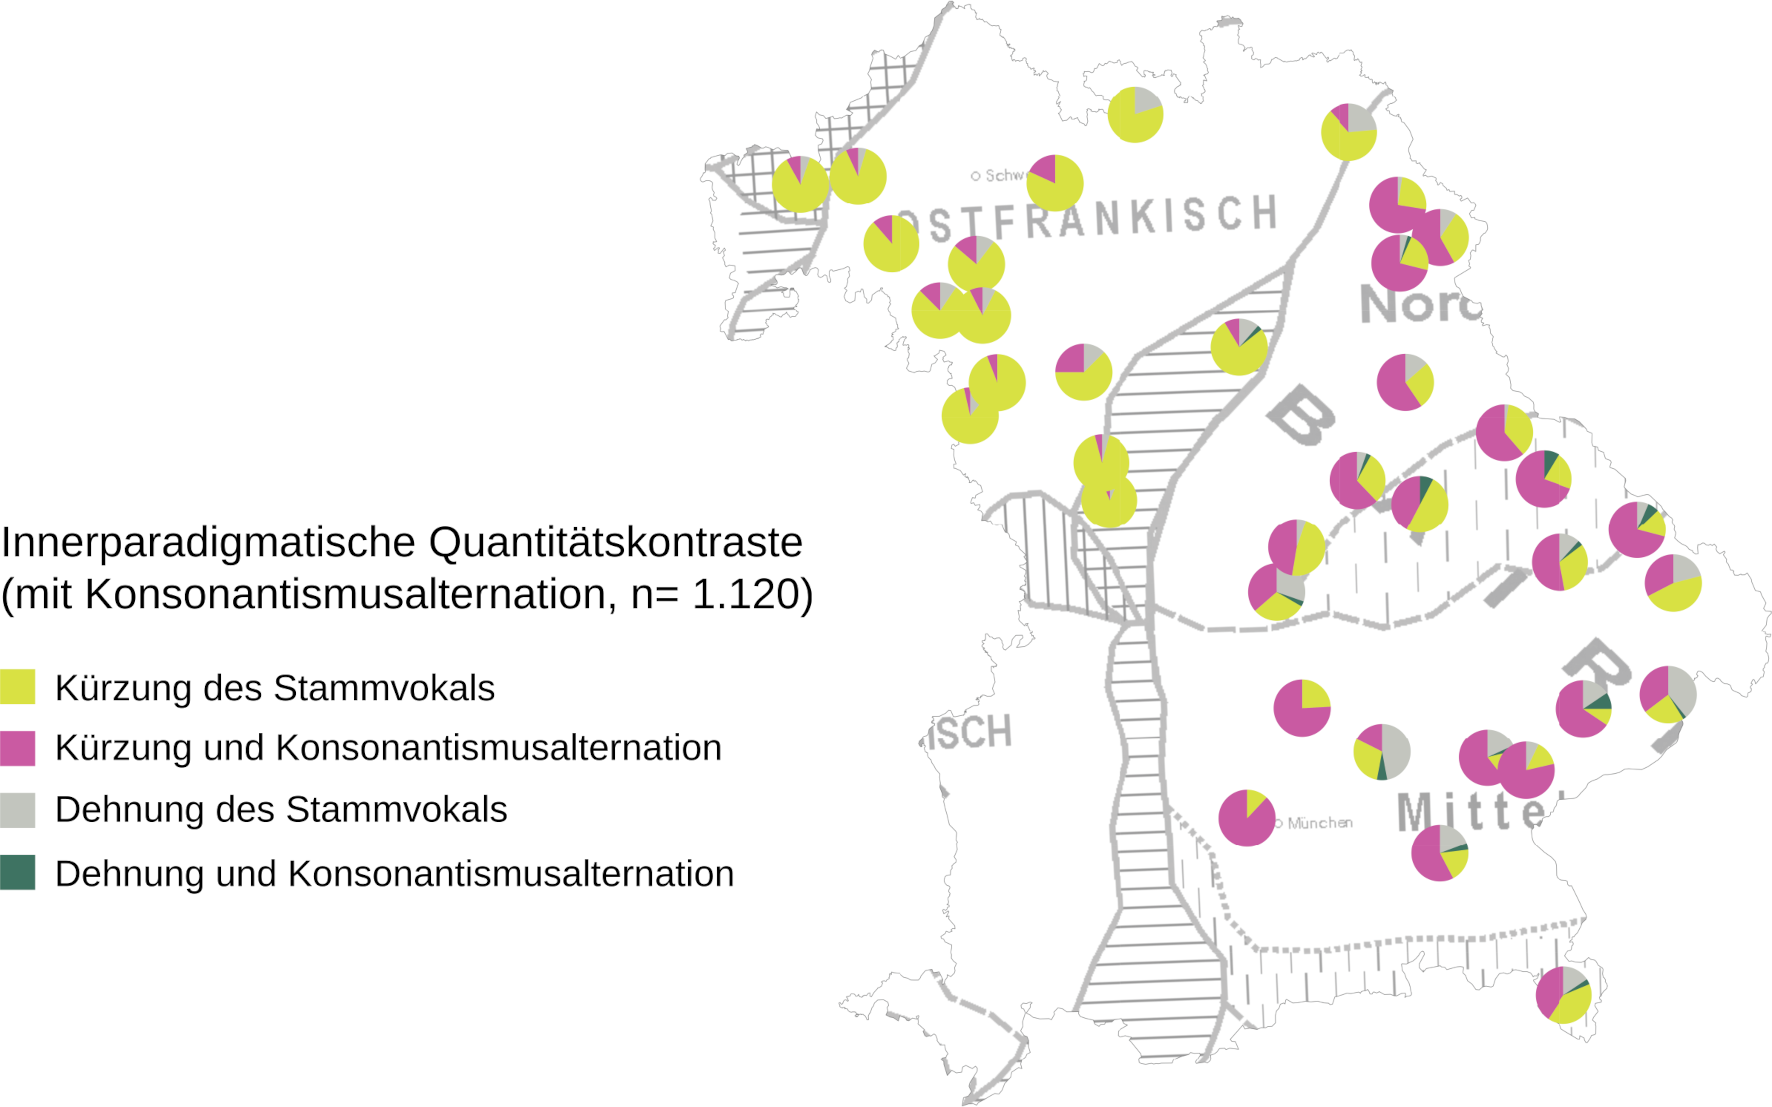
\includegraphics[width=\textwidth]{figures/Karte7.png}
\caption{Häufigkeitsverteilung verschiedener Realisierungen innerparadigmatischer Kontraste der Vokalquantität}
\label{map:7}
\end{map}
\vfill\pagebreak

\mapref{map:8} visualisiert die Häufigkeitsverteilung für Vokalquantitätswechsel des L-K-Musters (d.\,h. Kürzung) für die verschiedenen phonologischen Umgebungen im Auslaut von historischen Einsilbern mit altem Kurzvokal. Quan\-ti\-tät\-kon\-tras\-te bei Lexemen mit altem Kurzvokal vor Obstruent oder Affrikate sind zumeist großräumig belegt.\footnote{Dialektraumspezifisch sind nur die Quan\-ti\-tät\-kon\-tras\-te bei \textit{Brett} im Ofr. und \textit{Griff} im Nord- und Mittelbair., daneben sind sie im gesamten UG, allerdings nur vereinzelt bei \textit{Bett}, \textit{Bloch}, \textit{Fleck}, \textit{Joch}, \textit{Schaff}, \textit{Stadt} und \textit{Weg} belegt.} Vor bestimmten phonologischen Umgebungen, insbesondere bei altem Kurzvokal vor den Konsonantenfolgen /l/ und Konsonant sowie Nasal+Obstruent, sind Quantitätskontraste teilweise regelmäßig ausgeblieben.\footnote{Quantitätskontraste vor /l/ und Konsonant sind nur im nördlichen Nordbair. sowie im westlichen Ofr. zu finden, Einsilberdehnung vor Nasal+Obstruent ist teilweise im Ofr. sowie im nordbair. Tirschenreuth und im mittelbair. Kirchensur nicht belegt. Außerdem sind in den ofr. Tiefenbohrungspunkten Stadtschwarzach und Krum keine Quantitätskontraste in der Abfolge aus altem Kurzvokal und Affrikate belegt.}

Zu den Pluralformen historischer Einsilber zählen neben rein stammaffizierenden Markierungen (Typ fīš -- fiš ‚Fisch‘, frōš -- freš ‚Frosch‘) auch kombinierte Verfahren aus additiver Markierung und Modulation (Quantität, zum Teil in Kombination mit Alternationen der Vokalqualität). Bei zweisilbigen Pluralformen mit geschlossener Silbe sind die innerparadigmatischen Quantitätskontraste lautgesetzlich entstanden. Bei zweisilbigen Pluralformen mit offener Silbe hingegen ist im UG lautgesetzlich Dehnung in offener Tonsilbe eingetreten, allerdings finden sich auch hier im Ofr. und vereinzelt im Bair. innerparadigmatische Quantitätskontraste des L-K-Musters bei \textit{Grab} und \textit{Rad}, bei denen von morphologischen Quantitätskontrasten ausgegangen werden kann: \teuthoo{gro.2}{ɡrōͅ} -- \teuthoo{gre4?wA}{ɡrẹ̈wα} -- Dim. \teuthoo{gre24wAl}{ɡrẹ̄wαl} ‚Grab‘ (nordbair.-mittelbair. Blaibach), \teuthoo{ro2d}{rōd} -- \teuthoo{re):dEy}{re\klammeruntenpost{}{\doubleogonek}də⅄} -- Dim. \teuthoo{ra942dlA}{ra\klammeruntenpost{}̣̄dlα} ‚Rad‘ (ofr. Krum, vgl. \citealt[165]{Rowley1997} und \citealt[Karte 23]{SMF7}). Bemerkenswert ist dabei, dass die Quantitätskontraste hier zum Teil in Ortsdialekten belegt sind (nämlich im ofr. Wilhermsdorf und ofr. Ahorn), die im interdialektalen Vergleich in absoluten Zahlen nur wenige Formen mit Quantitätskontrasten aufweisen, wo diese Form der Pluralmarkierung also ein wenig frequentes Verfahren darstellt (\citealt[110]{SMF7}).


\begin{map}
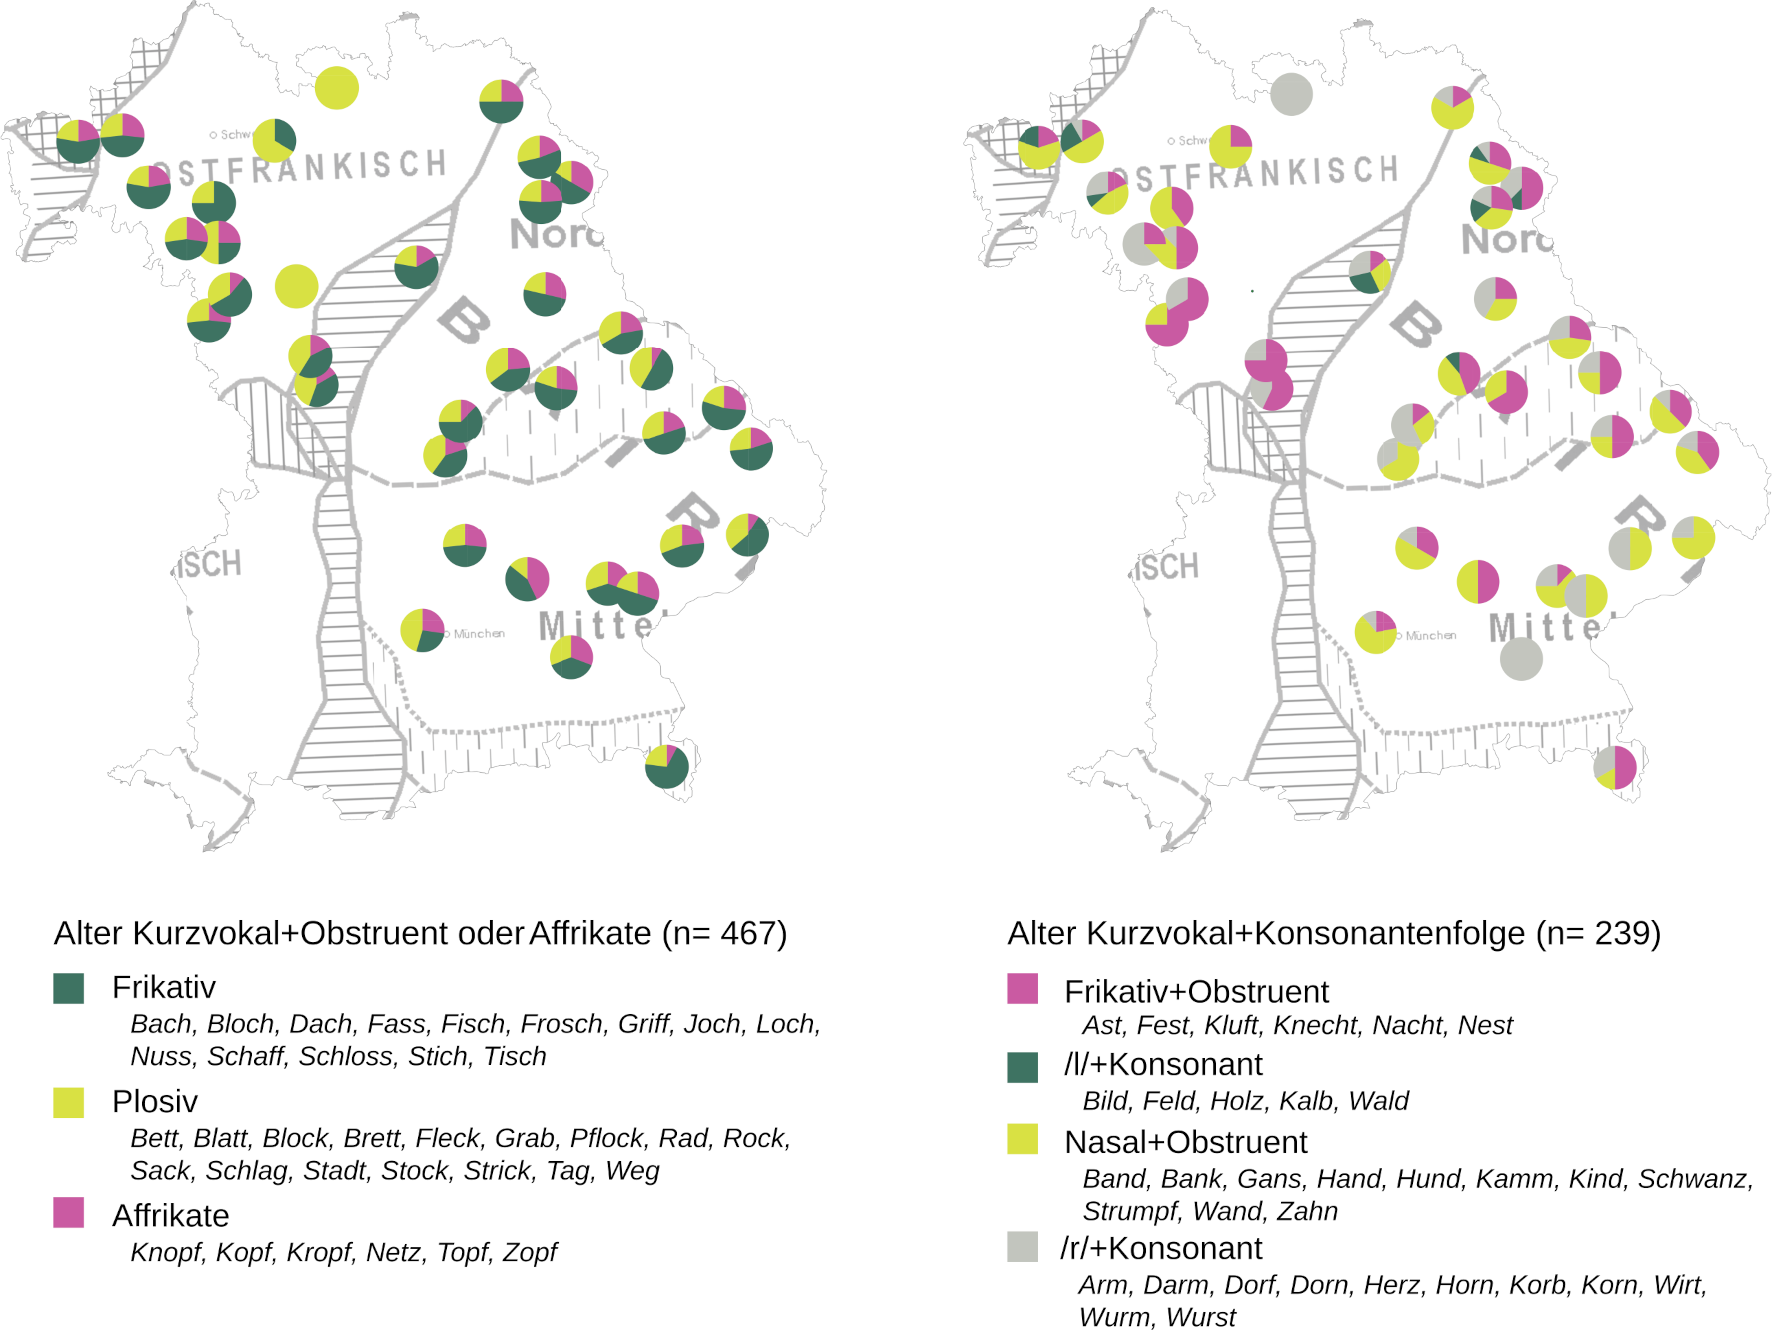
\includegraphics[width=\textwidth]{figures/Karte8.png}
\caption{L-K-Quantitätswechsel bei historischen Einsilbern mit altem Kurzvokal ($n=706$)\protect\footnote{In den BSA-Erhebungen wurde alter Kurzvokal vor Nasal in historischen Einsilbern nur in \textit{Sohn} (keine Belege für innerparadigmatische Quantitätskontraste) und \textit{Mann} (Kürzung in den ofr. und nordbair. Tiefenbohrungspunkten) abgefragt, weshalb diese Umgebung in der Kombinationskarte nicht berücksichtigt wurde. Ebenso nicht berücksichtigt wurde alter Kurzvokal+/l/, das nur in \textit{Stall} abgefragt wurde und im Ofr. sowie vereinzelt im Bair. belegt ist.}}
\label{map:8}
\end{map}

Neben Quantitätskontrasten in historischen Einsilbern mit altem Kurzvokal sind Quantitätskontraste auch bei historischen Einsilbern mit altem Langvokal oder Diphthong belegt (\mapref{map:9}). Während es Ortsdialekte gibt, die Quantitätskontraste bei altem Kurzvokal, nicht aber bei altem Langvokal oder Diphthong aufweisen (ofr. Mitteleschenbach und Hallerstein, bair. Inning am Holz), sind letztere in den Ortsdialekten im westlichen Ofr., im nördlichen Nordbair. sowie vereinzelt im Mittelbair. häufiger belegt. Die Durchsicht der Belege für die einzelnen Ortspunkte zeigt, dass innerparadigmatische Quantitätskontraste bei mhd. Langvokal oder Diphthong in der Tendenz nur vor jenen wortfinalen Konsonanten bzw. Konsonantenfolgen erscheinen, für die sie auch für alte Kurzvokale (d.\,h. als Ergebnis regulärer Einsilberdehnung) zu finden sind.\footnote{Nur in den mittelbair. Ortsdialekten Waldhof und Neukirchen am Inn ist bei \textit{Faust} ein Quantitätskontrast in der Umgebung vor Frikativ+Obstruent belegt, der für alte Kurzvokale nicht belegt ist.} Die phonologische Umgebung des auslautenden Konsonanten bzw. der Konsonantenfolge ist allerdings nur ein Faktor, um diese analogen Quantitätskontraste zu erklären. Insgesamt handelt es sich auch hier primär um lexemspezifische Entwicklungen mit z.\,T. großräumiger arealer Verteilung, so finden sich \textit{Faust}, \textit{Fuß}, \textit{Geiß}{ }und \textit{Haut} im Ofr. und Bair., \textit{Bauch} in den bair. Ortsdialekten, \textit{Schweif} im Mittelbair. und \textit{Stuhl} nur im Ofr.\footnote{In der Teilkarte zur arealen Verteilung wurden jene Lexeme nicht kartiert, die als einzige Vertreter eines mhd. Protovokals belegt sind: \textit{Vieh} (mhd. \textit{ie),} das mit Quantitätskontrast nur im ofr. Gebsattel belegt ist, \textit{Kloß} (mhd. \textit{ô}/\textit{o}, nur in SMF und SUF abgefragt) sowie \textit{Baum} (mhd. \textit{ou}), das im Unterofr. und vereinzelt im Nord- und Mittelbair. Quantitätskontraste aufweist.}


\begin{map}
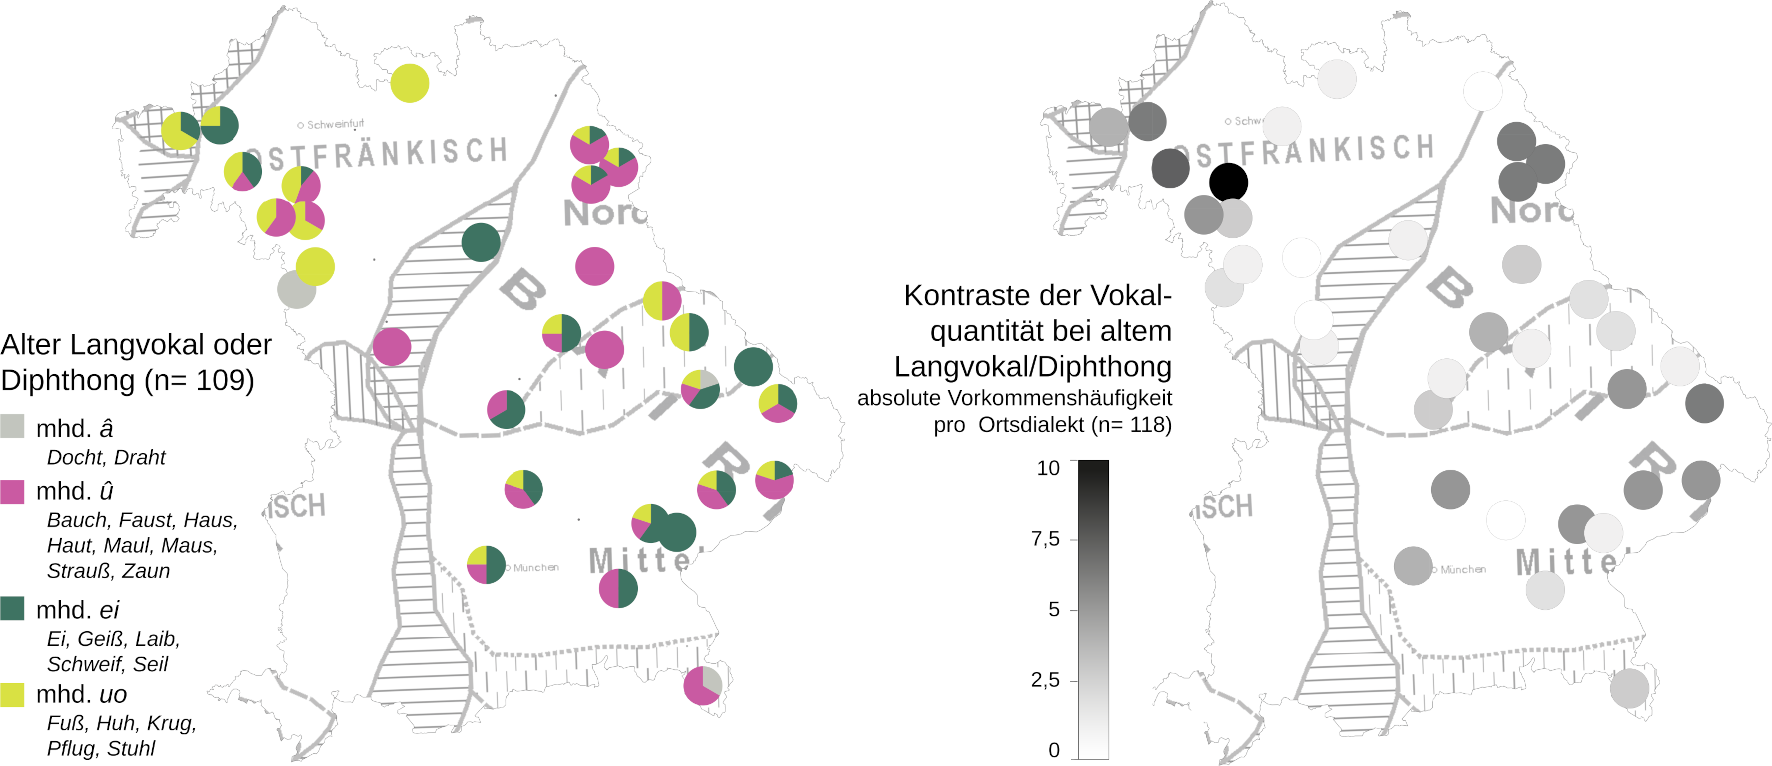
\includegraphics[width=\textwidth]{figures/Karte9.png}
\caption{Häufigkeitsverteilung und absolute Vorkommenshäufigkeit von L-K-Quantitätskontrasten bei altem Langvokal oder Diphthong in historischen Einsilbern}
\label{map:9}
\end{map}

Inwiefern stellen innerparadigmatische Quantitätskontraste nun ein produktives Pluralmarkierungsverfahren dar? Bei historischen Einsilbern mit altem Kurz- und Langvokal können mit Blick auf die BSA-Daten Quantitätsalternationen zwischen lexemspezifischen Lexikalisierungen und genereller Produktivität in Abhängigkeit von der Auslautkonsonanz verortet werden. Wie schwierig die Frage nach der Morphologisierung der Alternationen ist, ist daneben auch an innerparadigmatischen Quantitätskontrasten bei historischen Zwei- und Dreisilbern zu sehen. Die Belege innerparadigmatischer Quantitätsalternation bei historischen Mehrsilbern sind ausgesprochen heterogen, es handelt sich zumeist um vereinzelte Belege, die keine Arealbildung erkennen lassen. Schaut man wiederum auf die absolute Vorkommenshäufigkeit pro Ortsdialekt, so gibt es -- wie auch bei den analogen Quantitätskontrasten bei altem Langvokal oder Diphthong -- Ortspunkte, in denen morphologische Quantitätsalternationen bei historischen Mehrsilbern häufiger vorkommen (mit einem Schwerpunkt in einigen bair. Tiefenbohrungspunkten). In anderen Ortspunkten des UGs, die zwar Quantitätskontraste bei historischen Einsilbern kennen, sind sie für historische Mehrsilber nicht belegt, d.\,h. sie scheinen hier als Pluralmarkierungsverfahren nicht zur Verfügung zu stehen.


\begin{map}
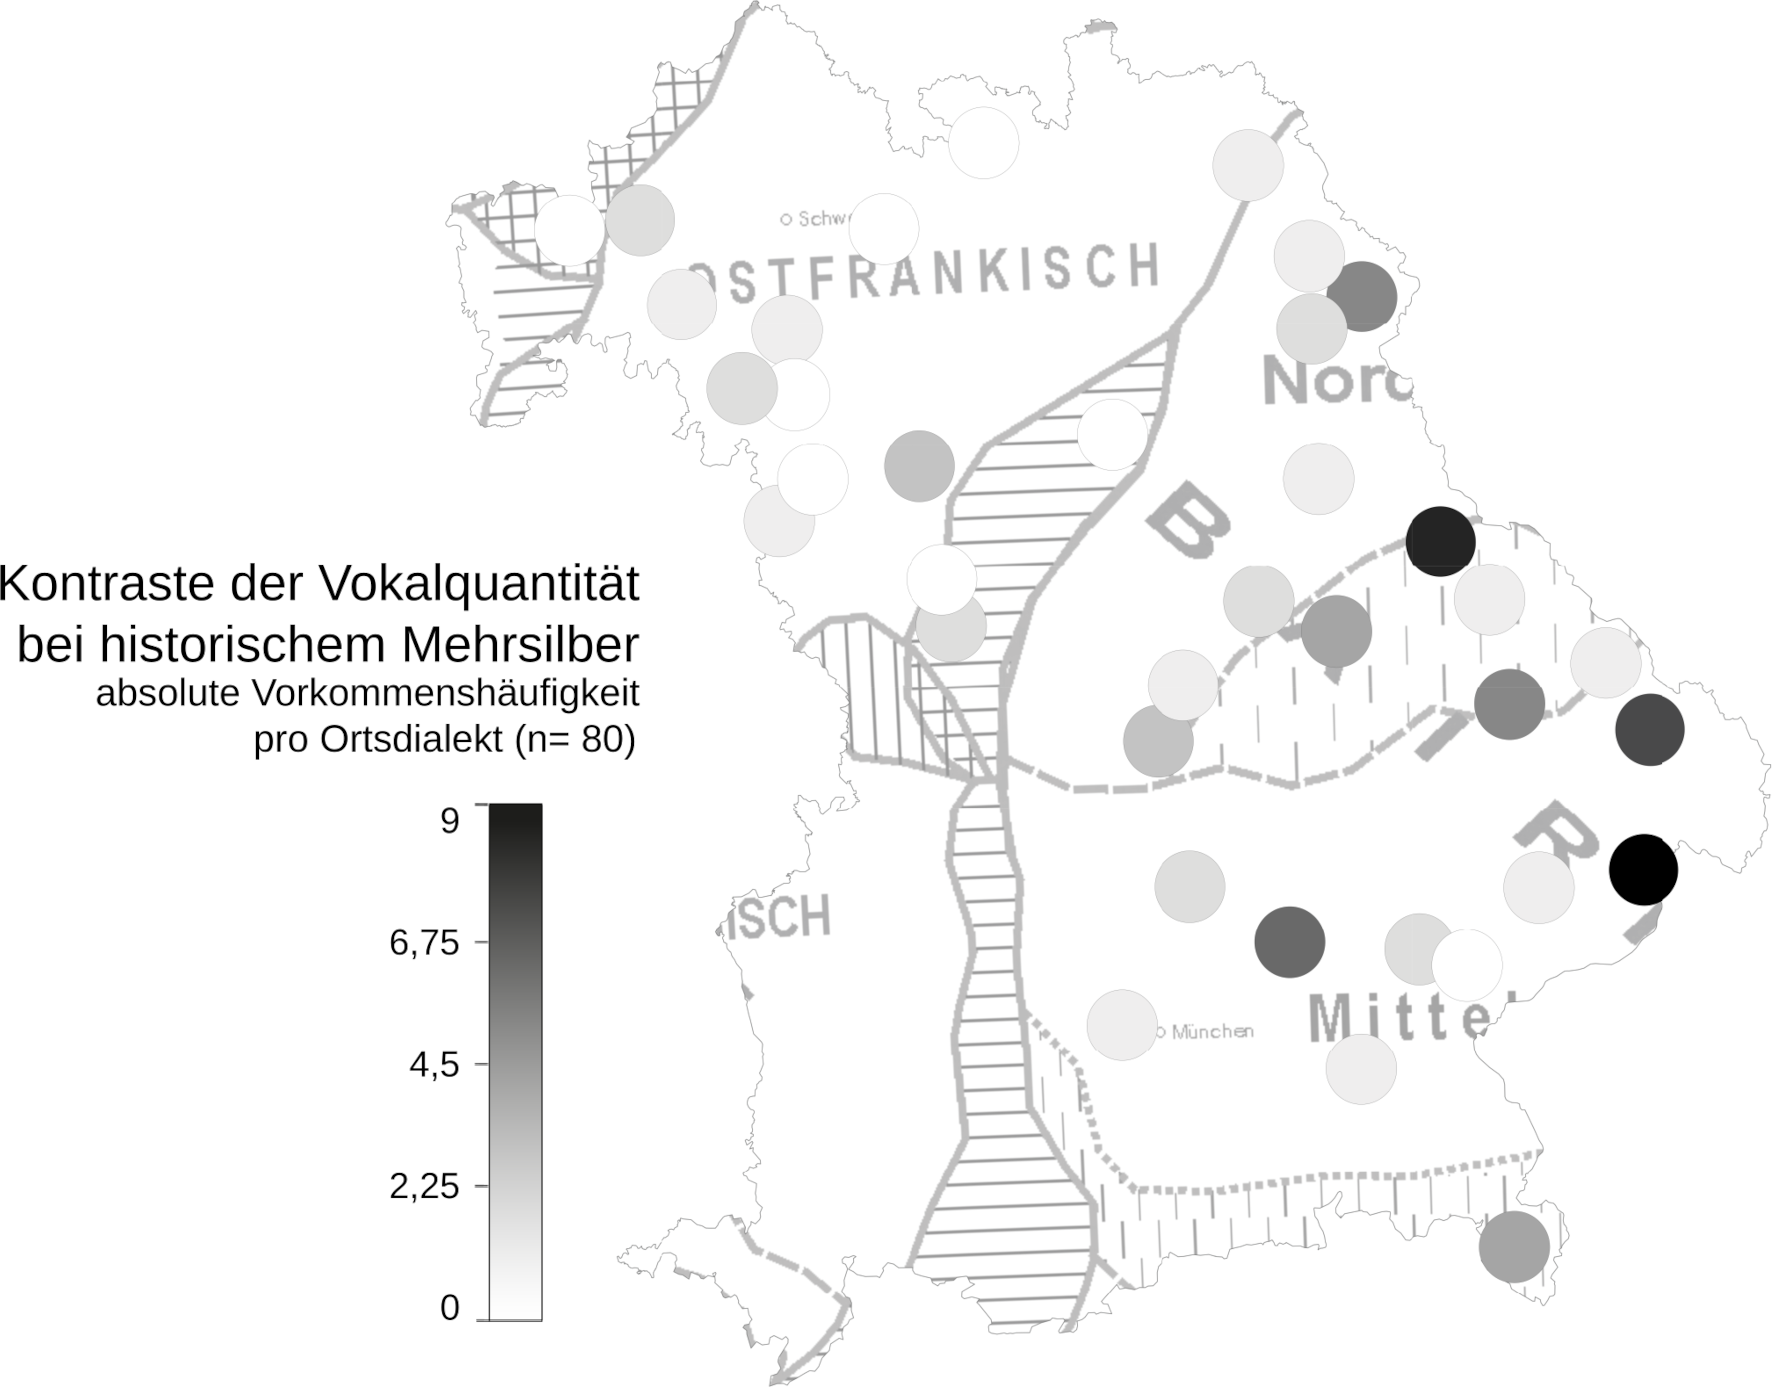
\includegraphics[width=\textwidth]{figures/Karte10.png}
\caption{Chloroplethkarte mit absoluter Vorkommenshäufigkeit von Quantitätskontrasten bei historischen Mehrsilbern}
\label{map:10}
\end{map}

\citegen{Kranzmayer1935} Darstellung zur Entwicklung historischer Zwei- und Dreisilber in oobd. Dialekten eröffnet eine diachrone Perspektive, die zumindest in Teilen eine Erklärung von Quantitätskontrasten bei historischen Mehrsilbern bietet. Lautgesetzlich entstehen im Frühmittelhochdeutschen innerparadigmatische Alternationen zwischen Langvokal in zwei\-silbigen Nominativ-Singular-Formen und Kurzvokal in dreisilbigen Nominativ-Plural-, Dativ-Singular- oder Diminutivformen, z.\,B. Nom.Sg. \teuthoo{va2tEr}{vātər} -- Dat.Sg. \teuthoo{vatEre}{vatəre} im Zimbrischen (vgl. das Vokalquantitätsmuster (c) in \tabref{tab:23}). Nach \citet[82]{Kranzmayer1935} war diese Entwicklung historisch „gemeinoberdeutsch“ und ist im Oobd. zumindest in Restformen bewahrt, darunter in der Region um Ries und Altmühltal sowie in einem oberfränkischen Gebiet um Ebermannstadt und Kulmbach (vgl. die Karte in \citealt[67]{Kranzmayer1935}). \citet[73]{Rowley1997} zufolge ist der lautgesetzliche Zustand in dessen nordostbayrischem UG nicht erhalten, in den vorliegenden Daten finden sich aber durchaus Belege für innerparadigmatische Alternationen bei his\-to\-ri\-schen Zwei- und Dreisilbern (\tabref{tab:24}).\largerpage[-1]

Inwiefern diese Belege tatsächlich einen konservierten lautgesetzlichen Zustand abbilden, muss offenbleiben. Die phonotaktische Umgebung der Erstsilbenkürze, die Dreisilbigkeit, verschwand durch die Apokope bereits im Mittelhochdeutschen in vielen Lexemen, die innerparadigmatische Alternation war damit nicht mehr transparent \citep[83]{Kranzmayer1935}. Gleichzeitig dokumentieren die Beispiele der \tabref{tab:24}, dass (vor der Folie des mhd. Protosystems) sowohl Lexeme mit additiver als auch stammaffizierender Pluralbildung mit innerparadigmatischen Quantitätskontrasten (teilweise in Kombination mit Lenis-Fortis-Kontrasten) belegt sind. Bei historisch starken Substantiven mit Umlautplural und bei historischen Zweisilbern ohne Änderung der Silbenanzahl in der flektierten Form liegen keine lautgesetzlich entstandene Quantitätsalternation vor.

Kranzmayers diachrone Modellierung der Vokalquantität in Abhängigkeit von der historischen Silbenanzahl kann indes einzelne Fälle synchroner Alternationen als konservierte Formen erklären. So deuten die Mehrfachbelege bei \textit{Gabel} darauf hin, dass die von Kranzmayer beschriebenen Verhältnisse im Oobd. großräumige Geltung hatten. Gleichzeitig können diese Formen ein Indiz für eine -- womöglich frühe -- Morphologisierung von Quantitätskontrasten bei zweisilbigen (neben einsilbigen) Stämmen in einzelnen Dialekten sein. Im Folgenden wird bei der Klassifikation von Quantitätskontrasten bei historischen Mehrsilbern konsequent eine synchrone Perspektive eingenommen und von einem morphologisierten Verfahren und analogischen Bildungen ausgegangen.


\begin{table}[p]
\caption{Innerparadigmatische Quantitätskontraste in historischen Zwei- und Dreisilbern im UG (Auswahl, $n=84$)\label{tab:24}}
\begin{subtable}{\textwidth}
\caption{historische Dreisilber\label{tab:24a}}
\small
\begin{tabularx}{\textwidth}{lllQ}
\lsptoprule
mhd. Flexion & {Singular} & {Plural}  & \\\midrule
 stswf. & \teuthoo{ga<vl}{ɡâvl} & \teuthoo{ga94vln}{ɡa\klammeruntenpost{}̣vln} &   ‚Gabel‘ (ofr. Gebsattel, daneben ofr. Pfofeld, mittelbair. Neukirchen am Inn, nordbair. Riedenburg, nordbair.-mittelbair. Grafenkirchen)\\
 \tablevspace
  & \teuthoo{v5e4<dA4}{v̩ệdα̣} & \teuthoo{ve4dAn}{vẹdαn} &   ‚Feder‘ (mittelbair. Inning am Holz)\\
  \tablevspace
 swstf. & \teuthoo{k,\_e2n}{k͓ʰēn} & \teuthoo{k,\_enAn}{k͓ʰenαn} &   ‚Kette‘ (nordbair.-mittelbair. Bernhardswald)\\
 \tablevspace
 stf. & \teuthoo{me.2d}{mēͅd} & \teuthoo{me.xd}{meͅxd} &   ‚Magd‘ (ofr. Stadtschwarzach, daneben ofr. Wilhermsdorf)\\
 \tablevspace
  & \teuthoo{gJo<A4s}{ɡ{\lkreis}ôα̣s} & \teuthoo{gJoA4s\%}{ɡ{\lkreis}oα̣s͈} &   ‚Geleise‘ (südbair.-mittelbair. Ramsau)\\
  \lspbottomrule
\end{tabularx}
\end{subtable}

\begin{subtable}{\textwidth}
\caption{historische Zweisilber mit altem Kurzvokal in offener Silbe\protect\footnote{Daneben belegt sind innerparadigmatische Quantitätskontraste bei \textit{Ader}, \textit{Auge}, \textit{Boden}, \textit{Faden}, \textit{Föhre}, \textit{Haken}, \textit{Hase}, \textit{Hemd}, \textit{Knoten}, \textit{Kröte}, \textit{Magen}, \textit{Name}, \textit{Nagel}, \textit{Säge}, \textit{Säule}, \textit{Schere}, \textit{Schnabel}, \textit{Speiche}, \textit{Stadel}, \textit{Stube}, \textit{Wade}, \textit{Wagen}.}}
\label{tab:24b}
\small
\begin{tabularx}{\textwidth}{llllQ}
\lsptoprule
\makecell[tl]{{mhd.}\\{Flexion}} & {Singular} & {Plural} & \makecell[tl]{Dimi-\\nutiv} & \\\midrule
 swm. & \teuthoo{gro42m}{ɡrọ̄m} & \teuthoo{gra4§(+m}{ɡrạ̃̆\klammerobenpost{}m} &  & ‚Graben‘ (mittelbair. Grafenau)\\
 \tablevspace
  & \teuthoo{bu2}{bū} & \teuthoo{bum}{bum} & \teuthoo{bi“bla}{bībla} & ‚Bube‘ (ofr. Hallerstein, daneben nordbair.-mittelbair. Bernried und Zwiesel)\\
  \tablevspace
 stm. & \teuthoo{he42vA}{hẹ̄vα} & \teuthoo{the4vA}{thẹvα} & \teuthoo{he42vErl}{hẹ̄vərl} & ‚Hafen‘ (nordbair.-mittelbair. Grafenkirchen)\\
 \tablevspace
  & \teuthoo{mae\$bru9.2dE}{mae̤bru\klammeruntenpost{}̄ͅdə} & \teuthoo{mae\$br{\textasciitilde}îidE}{mae̤br{\aufstrih}idə} &  & ‚Bruder‘ (ofr. Wilhermsdorf)\\
  \tablevspace
  & \teuthoo{vo.<ucl}{vôͅuXl} & \teuthoo{vo?.u?cl}{vöͅüXl} & \teuthoo{v5o?.u?cEli}{v̩öͅüXəli} & ‚Vogel‘ (ofr. Stadtschwarzach, daneben nordbair.-mittelbair. Bernhardswald)\\
  \tablevspace
 swf. & \teuthoo{Ata.2om}{αtāͅom} & \teuthoo{ta.om}{taͅom} &  & ‚Taube‘ (nordbair.-mittelbair. Grafenkirchen, daneben mittelbair. Waldhof)\\
 \tablevspace
 swstf. & \teuthoo{no2l}{nōl} & \teuthoo{noln}{noln} &  & ‚Nadel‘ (mittelbair. Grafenau, daneben mittelbair. Inning am Holz)\\
 \lspbottomrule
\end{tabularx}
\end{subtable}
\end{table}


\begin{table}
\ContinuedFloat
\caption{Innerparadigmatische Quantitätskontraste in historischen Zwei- und Dreisilbern im UG (Auswahl, $n=84$)}
\begin{subtable}{\textwidth}
\caption{historische Zweisilber mit altem Kurzvokal in geschlossener Silbe\protect\footnote{Daneben bei \textit{Birne}, \textit{Borste}, \textit{Furche}, \textit{Henne}, \textit{Karren}, \textit{Katze}, \textit{Lärche}, \textit{Ratte}, \textit{Rippe}, \textit{Tochter}, \textit{Wanne}, \textit{Wespe}.}}
\label{tab:24c}
\small
\begin{tabularx}{\textwidth}{lQQl>{\raggedright\arraybackslash}p{.4\textwidth}}
\lsptoprule
\makecell[tl]{mhd.\\Flexion} & {Singular} & {Plural} & {Diminutiv} & \\\midrule
  swm. & \teuthoo{s\#li.“4n}{šlị̄ͅn} & \teuthoo{s\#lin}{šlin} &  & ‚Schlitten‘ (mittelbair. Neukirchen am Inn)\\
  \tablevspace
  & \teuthoo{gðo<At}{ɡ̩ôαt}-\teuthoo{n@}{n̥} & \teuthoo{gða)\$t}{ɡ̩a\klammeruntenpost{}̤t}-\teuthoo{n@}{n̥} & \teuthoo{ga4rtl}{ɡạrtl} & ‚Garten‘ (mittelbair. Grafenau, daneben nordbair. Tirschenreuth)\\
  \tablevspace
 stm. & \teuthoo{ho:"(+mEr}{hō{\doubleogonek}̃\klammerobenpost{}mər} & \teuthoo{ha94mr}{ha\klammeruntenpost{}̣mr} &  & ‚Hammer‘ (ofr. Stadtschwarzach)\\
 \tablevspace
 stf. & \teuthoo{b\_mu.<AtA}{bʰmûͅαtα} & \teuthoo{mu.AtAn}{muͅαtαn} &  & ‚Garten‘ (mittelbair. Niedertaufkirchen, daneben nordbair.-mittelbair. Grafenkirchen, mittelbair. Inning am Holz)\\
 \tablevspace
 stswf. & \teuthoo{se42NSd}{sẹ̄ŋʃd} & \teuthoo{dse4NSdn@}{dsẹŋʃdn̥} &  & ‚Sense‘ (nordbair. Kallmünz, daneben nordbair.-mittelbair. Grafenkirchen, mittelbair. Neukirchen am Inn)\\
 \tablevspace
  & \teuthoo{wu.(<Ed5s5ý@}{wûͅ\klammerobenpost{}əd̩s̩ɫ̥} & \teuthoo{wi.Et,S,ý@}{wiͅət͓ʃ͓ɫ̥} &  & ‚Wurzel‘ (nordbair. Groschlattengrün, daneben nordbair. Oberdolling)\\
  \tablevspace
 swf. & \teuthoo{mu<g-N@}{mûɡ{}͐ŋ̥} & \teuthoo{muk-N@}{muk{}͐ŋ̥} &  & ‚Mücke‘ (mittelbair. Grafenau)\\
\lspbottomrule
\end{tabularx}
\end{subtable}
\end{table}


\subsubsection{Konsonantismuskontraste}\label{sec:7.1.2.3}\largerpage[-1]
Neben Alternationen im Paradigma, die durch Kontraste der Vokalqualität oder -quantität entstehen, affizieren andere Alternationsmuster den Konsonantismus des Stammes. Konsonantismuskontraste finden sich im Auslaut des Stammes und damit an einer Stelle, die -- anders als der Stammvokal -- „für morphologische Symbolisierung nicht primär vorgesehen“ ist \citep[284]{Harnisch1994a}. Phänomene des Konsonantismus werden im Folgenden konsequent aus der -- zugegebenermaßen engen, aber für die Forschungsfrage relevanten -- Perspektive der Flexionsmorphologie behandelt. Der Anspruch ist daher nicht, historische Entwicklungen des Konsonantismus vollständig darzustellen, sondern Ziel ist es, phonetisch-phonologische Entwicklungen aufzuzeigen und zu diskutieren, inwiefern diese für die Kodierung der flexivischen Information funktionalisiert sind. Die Kernfrage des Kapitels lautet folglich: Wann ist lautliche Variation im Konsonantismus zwischen Singular- und Pluralform auf der pho\-ne\-tisch-pho\-no\-lo\-gisch\-en Ebene anzusiedeln, weil sie beispielsweise durch die phonotaktische Position eines Konsonanten in der Wortform bedingt ist? Und wann entsprechen mal isolierte, mal großräumigere Fälle von innerparadigmatischen Konsonantismusalternationen einem Pluralmarkierungsverfahren und damit diachron einer morphologischen Funktionalisierung?


\begin{figure}
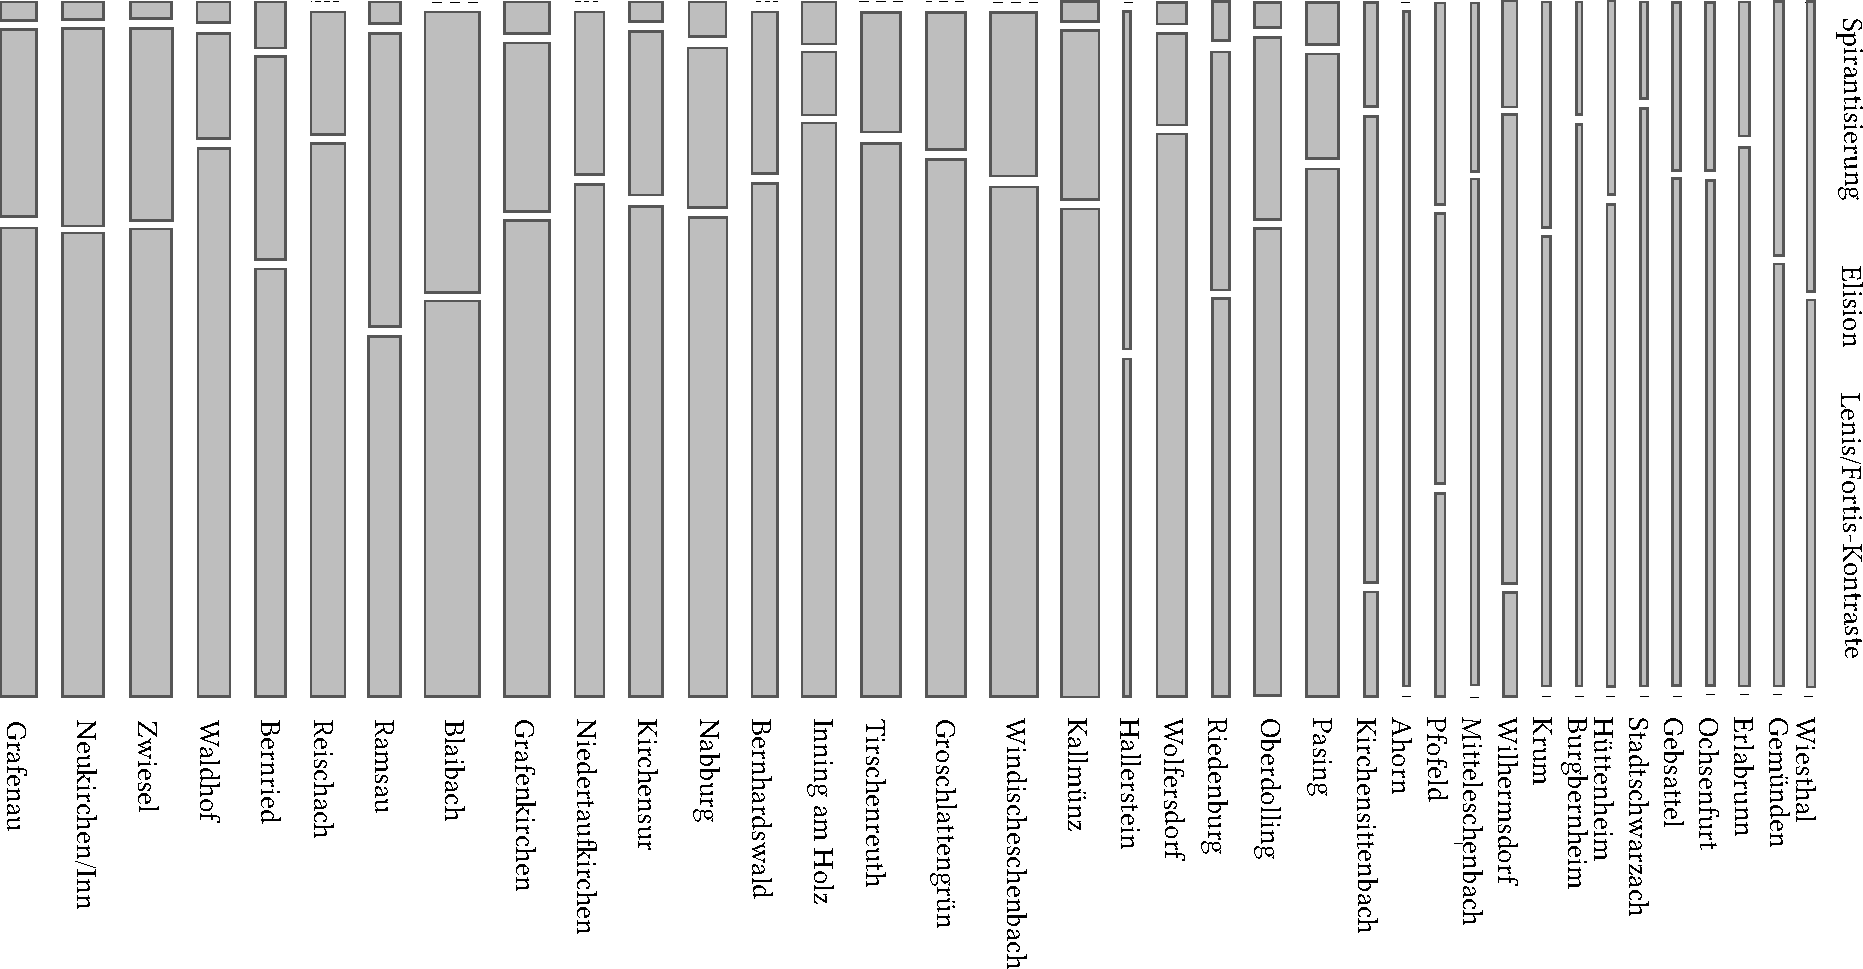
\includegraphics[height=.75\textwidth,angle=90]{figures/revisedNickelNominalmorphologie-img018.pdf}
\caption{Mosaik-Plot mit Häufigkeitsverteilung innerparadigmatischer Konsonantismuskontraste ($n=875$)}
\label{fig:5}
\end{figure}

Innerparadigmatische Konsonantismusalternationen sind -- wie auch die anderen bisher vorgestellten stammaffizierenden Verfahren -- das Ergebnis phonologischer Prozesse. Diese Prozesse sind im Bereich des Konsonantismus in den ofr. und bair. Dialekten unterschiedlich verlaufen (exemplarisch sind hier die sogenannte binnenhochdeutsche und die mittelbair. Konsonantenschwächung zu nennen), woraus auch synchron eine Zweiteilung des UGs resultiert -- sowohl bezogen auf das phonologische als auch auf das zur Verfügung stehende flexionsmorphologische Inventar. Dass es hinsichtlich der verschiedenen Typen von innerparadigmatischen Konsonantismuskontrasten und ihrer relativen Häufigkeit dialektspezifische Unterschiede gibt, illustriert \figref{fig:5}. Das Mosaik-Plot visualisiert die Variablen Ortsdialekt (von West nach Ost), Typus der Konsonantismusalternation und absolute Häufigkeit. Anhand der Größe der Flächen der Rechtecke ergibt sich, dass innerparadigmatische Konsonantismusalternationen in den nord- und mittelbair. Tiefenbohrungspunkten weitaus häufiger belegt sind als in den ofr. Daneben zeigt die Verteilung der verschiedenen Typen, dass es eine dialektspezifische Markierungsstrategie gibt: Lenis-Fortis-Kontraste finden sich nur im Bair. (\sectref{sec:7.1.2.3.1}). Und auch bei innerparadigmatischen Alternationen zwischen elidiertem und erhaltenem Konsonanten gibt es im Bair. spezifische Flexionsmuster, wie in \sectref{sec:7.1.2.3.2} gezeigt wird.

Wie schwierig die Grenzziehung zwischen synchron aktivem phonetisch"=phonologischem Prozess und der Morphologisierung von Konsonantismusalternationen ist, ist exemplarisch an der vokalischen vs. konsonantischen Realisierung von Liquiden zu sehen (\tabref{tab:25}). Im Datenmaterial gibt es Singular- und Pluralformen, bei denen sich durch die additive Markierung der Pluralform innerparadigmatische Alternationen im Stammauslaut zwischen vokalisch realisiertem Liquid im Singular und in intervokalischer Position konsonantisch realisiertem Liquid im Plural ergeben. Die Belege stammen aus dem bair. Teil des UGs, d.\,h. dem Gebiet /l/-Vokalisierung und der konsequenten /r/-Vokalisierung (d.\,h. systematische Vokalisierung von /r/ im absoluten Auslaut wie in \textit{Jahr} und im Auslaut vor Konsonant, z.\,B. \textit{Berg}, \textit{Turm}).\footnote{Die Erhebungen im Rahmen des \textit{Bayerischen Sprachatlas} haben ergeben, dass sich das von \citet{Kranzmayer1956} beschriebene Gebiet der konsequenten \textit{r}{}-Vokalisierung „deutlich nach Westen, teilweise bis an den Lech“ verschoben hat (\citealt[65]{RennKönig2006}). Für das Lexem \textit{Tor} (Typ \teuthoo{do.}{doͅ} -- \teuthoo{dorA}{dorα} oder \teuthoo{deArA}{deαrα}) finden sich daneben auch Belege im Ofr. (vgl. \citealt[§34c4, §49c3 und Karte 26]{Kranzmayer1956}, \citealt[82]{Rowley1997} sowie \citealt[60--99]{SMF4} zur \textit{r}{}-Realisierung im Ofr.).}


\begin{table}
\begin{tabular}{llll}
\lsptoprule
 & {Singular} & {Plural} & \\\midrule
{/r/} & \teuthoo{gs\#i4"4A}{ɡšị̣̄α} & \teuthoo{gs\#i4"4ArA}{ɡšị̣̄αrα} & ‚Geschirr‘ (Kirchensittenbach)\\
& \teuthoo{o.2A4}{ōͅα̣} & \teuthoo{o.2A4rA}{ōͅα̣rα} & ‚Ei‘ (Grafenau)\\
& \teuthoo{s\#do.2dl@do2A}{šdōͅdl̥dōα} & \teuthoo{de2ArA}{dēαrα} & ‚Tor‘ (Nabburg)\\
& \teuthoo{diE}{diə} & \teuthoo{diErAn}{diərαn} & ‚Tür‘ (Blaibach)\\
\tablevspace
{/l/} & \teuthoo{s5ma4<i.}{s̩mậiͅ} & \teuthoo{b-ma4<i.lA}{b{}͐mậiͅlα} & ‚Maul‘ (Grafenau)\\
\lspbottomrule
\end{tabular}
\caption{Beispiele für innerparadigmatische Alternation bei Liquid im absoluten Auslaut in der Singular- und in intervokalischer Position in der Pluralform\label{tab:25}}
\end{table}

In diesen Singular- und Pluralformen ist die Realisierung der Liquiden durch die jeweilige Position in der Wortform bedingt und in der Folge vorhersagbar, Vokalisierung und konsonantische Realisierung von /l/ und /r/ können als Allophone klassifiziert werden. Eine ähnliche Lösung bietet sich auch für intervokalische Spirantisierungen an (\sectref{sec:7.1.2.3.3}) und für additive Formen mit erhaltenem Obstruenten (\sectref{sec:7.1.2.3.2}). Formenbildung an der Schnittstelle zwischen Phonologie und Morphologie ist hier stärker in der Phonologie zu verorten und primär durch phonologische Prozesse gesteuert. Gleichzeitig erscheinen die Alternationen sehr regelmäßig in Flexionsformen, sodass sie durchaus als „begleitende“ morphophonologische Marker funktionalisiert sein könnten und als solche perzipiert werden (und entsprechend kognitiv verankert sind).

\subsubsubsection{Lenis-Fortis-Kontraste}
\label{sec:7.1.2.3.1}
\begin{quote}
Die Darstellung der Quantität ist das Einfachste und zugleich das Schwierigste in der bair. mda. [Mundart, GN]. \citep[12]{Kollmer1949}
\end{quote}

Im bair. Teil des UG sind innerparadigmatische Kontraste zwischen Lenis- und Fortisobstruenten durch das sogenannte „bairische Silbengesetz“ (auch Pfalzsche Regel, vgl. \citealt{Pfalz1913, Pfalz1936}) bedingt: Im Auslaut der Haupttonsilbe folgt Leniskonsonanz auf Langvokal, auf Kurzvokal hingegen Fortiskonsonanz (vgl. 	\tabref{tab:26}). Die Opposition zwischen Lenis- und Fortis-Konsonant besteht dabei weniger in einem Kontrast der Konsonantenstärke als vielmehr in einem Kontrast der Konsonantenquantität (vgl. \citealt[33--35]{Bachmann2000}, \citealt[30]{Hinderling1980}, \citealt[177]{Kufner1957}, \citealt[14]{Schießl1909}, \citealt[240]{Seiler2009} sowie \citealt[30]{Auer1991}).


\begin{table}
\begin{tabular}{llll}
\lsptoprule
 Langvokal\,+\,Leniskonsonanz & \multicolumn{2}{l}{Kurzvokal\,+\,Fortiskonsonanz} & \\
 {VːC\textsubscript{lenis}} & \multicolumn{2}{c}{VC\textsubscript{fortis}} & \\\cmidrule(lr){1-1}\cmidrule(lr){2-3}
 Nom.Sg. & Nom.Pl. & Diminutiv & \\  \midrule
 \teuthoo{gri“v}{ɡrīv} & \teuthoo{grI3f}{ɡrı̆f} &  & ‚Griff‘\\
 \teuthoo{hu<nd}{hûnd} & \teuthoo{hu3nt\_}{hŭntʰ} & \teuthoo{hu3ntÿ}{hŭnt\ɫ} & ‚Hund‘\\
 \teuthoo{di“s\#5}{dīš̩} & \teuthoo{dI3S}{dı̆ʃ} &  & ‚Tisch‘\\
\cmidrule(lr){1-2}
\multicolumn{2}{c}{ {Minimalpaare}} &  & \\
\lspbottomrule
\end{tabular}
\caption{Beispiele für innerparadigmatische Lenis-Fortis-Kontraste mit Minimalpaaren aus dem nordbair. Groschlattengrün}
\label{tab:26}
\end{table}

Die Lenis-Fortis-Opposition ist ein Spezifikum des nord- und mittelbair. Teils des UGs, und zwar sowohl aus phonologischer als auch aus flexionsmorphologischer Perspektive. \citet[59]{Seidelmann2013} sieht in dem Kontrast zwischen Lenis und Fortis denn auch „die zentrale Opposition im phonologischen System des Mittelbairischen“ und die sog. mittelbairische und die binnenhochdeutsche Konsonantenschwächung als „zwei konträr organisierte Systeme“ (\citealt[60]{Seidelmann2013}, vgl. \citealt[34--35]{Steger1968}). Infolge der verschiedenen phonologischen Prozesse, die nach \citet[§34]{Kranzmayer1956} zur „mittelbair. Konsonantenschwächung“ gezählt werden (darunter die Lenisierung von Fortes im In- und Auslaut nach Langvokal, vgl. \tabref{tab:33}), sind Vokal- und Konsonantenquantität im Nord- und Mittelbair. korreliert. Im Ofr. hingegen ist die distinktive Opposition zwischen mhd. Lenes und Fortes als Ergebnis der binnenhochdeutschen Konsonantenschwächung in allen Positionen aufgehoben; in Minimalpaaren wie ofr. \teuthoo{vI2s\#}{vı̄š} -- \teuthoo{vis\#}{viš} ‚Fisch‘ ist der Kontrast der Vokalquantität das relevante Merkmal.


\begin{map}
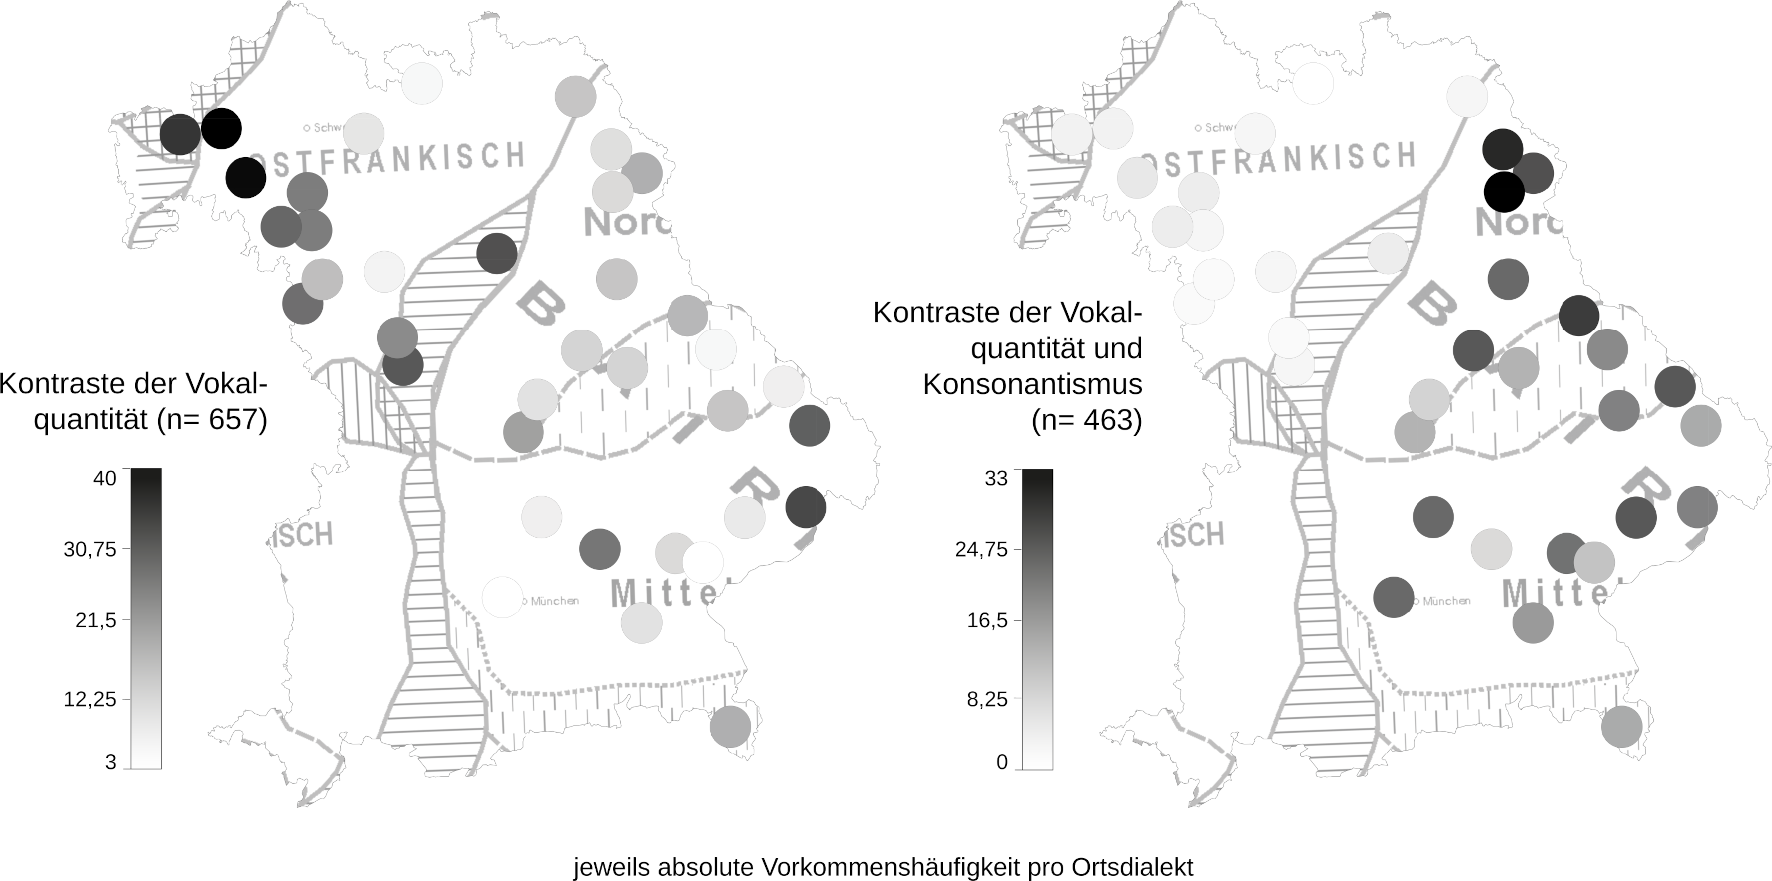
\includegraphics[width=\textwidth]{figures/Karte11.png}
\caption{Chloroplethkarten zur absoluten Vorkommenshäufigkeit von Quantitätskontrasten vs. Quantitäts- und Konsonantismuskontrasten ($n=1.120$)}
\label{map:11}
\end{map}

Synchron spiegelt sich die divergente Entwicklung der phonologischen Systeme im Ofr. und im Nord- und Mittelbair. hinsichtlich Vokalquantität und Konsonantismus in den stammaffizierenden Pluralmarkierungsstrategien wider. Die Chloroplethkarten in \mapref{map:11} illustrieren, dass es für die absoluten Häufigkeiten stammaffizierender Pluralmarkierungen, die die Quantität von Stammvokal sowie von in- und auslautendem Konsonantismus betreffen, in der Tendenz eine Zweiteilung gibt: Während sich Kontraste der Vokalquantität in allen Tiefenbohrungspunkten, schwerpunktmäßig aber in den Ortspunkten des westlichen Ofr. finden, sind Kontraste, die die Vokalquantität in Kombination mit Lenis-Fortis-Kontrasten betreffen, nur in den bair. Ortsdialekten nachweisbar.

Ausgangspunkt aller Analysen zum Phänomen -- diachroner wie synchroner -- sind die rezenten Quantitätsverhältnisse im Nord- und Mittelbair. „Unkontrovers“ ist laut \citet[343]{MoosmüllerScheutz2018}, dass diese aus einer zweimorigen Silbenstruktur resultieren und ein Beispiel von „mora compensation“ \citep[1080]{Auer1989} darstellen, d.\,h. von kompensatorischem Quantitätenausgleich im phonologischen Wort.\footnote{In Einsilbern folgt Morenkompensation auf der Wortebene denselben Prinzipien wie bei Morenkompensation in der Silbe \citep[1082]{Auer1989}.} In der Silbe sind die Quantitäten von Vokal und Konsonant komplementär zueinander verteilt: Auf einen kurzen (einmorigen) Vokal folgt ein Fortiskonsonant (dieser entspricht einer einmorigen Geminate),\footnote{Geminate wird hier und im Folgenden in der Definition von \citet[108]{Seiler2005} verwendet, „i.e., a geminate is a consonant that is underlyingly moraic and phonetically long [\ldots].“ Geminaten in dieser Definition können im Inlaut (ambisilbisch) und wortfinal im Auslaut erscheinen.}  auf einen langen (zweimorigen) Vokal folgt ein nicht-morenwertiger Leniskonsonant bzw. -Konsonantencluster (vgl. \citealt[342]{MoosmüllerScheutz2018}, \cites[113]{Seiler2005}[260]{Seiler2009}).\footnote{In dem Artikel „Some ways to count morae“ zählt \citet[1090]{Auer1989} anders, da das phonologische Wort im Bair. drei Moren umfasse (ebenso \citealt[35]{Hinderling1980}). In einer Wortform wie [re:d] ‚rede (1.Ps.Sg.Präs.)‘ ist der Langvokal danach zweimorig, der Leniskonsonant einmorig (vgl. \citealt[11]{Auer1991}). Auers morentheoretische Analyse unterscheidet sich außerdem dahingehend, dass Geminaten nicht wortfinal erscheinen können und daher regelbasiert reduziert werden (\citealt[1093]{Auer1989}, vgl. \citealt[14]{Auer1991}). Wortformen mit wortfinaler Geminate wie Pl.
\textit{fischsch} ‚Fisch‘ modelliert \citet[1094--1095]{Auer1989} in ihrer lexikalischen Repräsentation mit einer leeren More, die einem Silbenkern entspricht und nicht durch ein Segment besetzt wird.}\largerpage

Kontrovers ist hingegen, welches der beiden korrelierenden Merkmale Träger der Merkmalsopposition und welches phonologisch nicht distinktiv ist. Dialektologische Arbeiten mit (morpho)phonologischem Schwerpunkt (\citealt{Dozauer1967}, \citealt{HarnischRowley1990}, \citealt{Hinderling1980}, \citealt{Kufner1957}, \citealt{Rowley1997}, \citealt{Wiesinger1990}) sehen das relevante Merkmal in der Lenis-Fortis-Opposition, die Vokallänge dagegen ist allophonisch (hierzu kritisch \citealt[355]{MoosmüllerScheutz2018}). \citet{Bannert1976} bietet mit seinen instrumentellen Quantitätsmessungen eine frühe empirische Untersuchung und ein zweites Erklärungsmodell, das nicht die Lenis-Fortis-Opposition, sondern eine prosodische Größe als phonologisch distinktives Merkmal definiert: die komplementäre Relation von Vokal und Konsonant. Vokal und Folgekonsonant werden in dieser Analyse als eine Einheit aufgefasst, deren jeweilige Anteile sich in der Lenis- vs. Fortisrelation komplementär zueinander verhalten; unabhängig von der absoluten Dauer ist die komplementäre Relation konstant groß.\footnote{Die Grundstruktur der komplementären Länge zwischen Vokal und nachfolgendem Konsonanten beträgt im Verhältnis im Lenisfall 3:1, im Fortisfall 2:3 \citep[87]{Bannert1976}. Die Analyse einer komplementären Länge von Vokal und Konsonant findet sich als Konzept des Silbenschnitts bereits bei \citet{Sievers1976}, \citet{Pfalz1913} oder -- aus strukturalistischer Perspektive -- bei \citet{Trubetzkoy1977}.}

Wie die rezenten Quantitätsverhältnisse als Spezifikum des Nord- und Mittelbair. diachron entstanden sind, rekonstruiert \citet{Seiler2005, Seiler2008, Seiler2009} mit einer phonologischen Analyse der Lautwandelprozesse. In Seilers Interpretation stellt auch der Konsonantismus, genauer: dessen Morenwertigkeit, eine Bedingung für Veränderungen der Vokalquantität und folglich das relevante Merkmal dar \citep[267]{Seiler2009}. Die innerparadigmatische Alternation zwischen Lang\-vo\-kal\,+\,Le\-nis und Kurz\-vo\-kal\,+\,For\-tis ist das Ergebnis verschiedener regulärer Lautveränderungen (\cites[187]{Seiler2008}[244--245]{Seiler2009}, vgl. \citealt[§34k2-3]{Kranzmayer1956}):\largerpage

\begin{itemize}
\item \textit{Finale} \textit{Geminatenkürzung}: Im absoluten Auslaut erfolgte Kürzung (auch Lenisierung) von Geminaten (Sg. \teuthoo{tiS'S'}{tiʃ̌ʃ̌} > \teuthoo{tiS'}{tiʃ̌} ‚Tisch‘, vgl. auch \citealt[20--21]{Lessiak1933}). Infolge der Apokope des Schwa der Pluralform (Pl. \teuthoo{tiS'S'E}{tiʃ̌ʃ̌ə} > \teuthoo{tiS'S'}{tiʃ̌ʃ̌}) entsteht die innerparadigmatische Alternation zwischen Lenis im Singular und Fortis (d.\,h. Geminate) im Plural (vgl. \citealt[1098]{Wiesinger1983a}).
\item \textit{Einsilberdehnung}: Vokale in Einsilbern werden gedehnt, wenn ein einzelner Konsonant in der Silbenkoda folgt (dabei spielt es keine Rolle, ob der Einzelkonsonant das Ergebnis von finaler Geminatenkürzung ist, vgl. \citealt[259]{Seiler2009}). Den Erklärungsansatz liefert die Morentheorie im Sinne von \citet{Hayes1989}: Dialekte, die Einsilberdehnung durchgeführt haben, haben eine mindestens zweimorige Silbenstruktur (vgl. \citealt[259]{Seiler2009}). Ist der Konsonant nicht-morenwertig, wird der einmorige Kurzvokal zu einem zweimorigen Langvokal gedehnt.
\item \textit{Reanalyse} \textit{und} \textit{„analogical} \textit{grammar} \textit{simplification“} \citep[122]{Seiler2005}: Da „\textit{most} long vowels“\footnote{Wenngleich diese frequenzbasierte Annahme plausibel scheint, fehlt m.\,E. die Fundierung durch tatsächliche Frequenzwerte. Grundsätzlich fällt in der Diskussion um die bair. Quantitätsverhältnisse auf, dass sich die Forschungsdiskussion in weiten Teilen auf dieselben Beispielbelege in \citet{Pfalz1913, Pfalz1936} und \citet{Kufner1957} bezieht (vgl. die Kritik in \citealt[344]{MoosmüllerScheutz2018} sowie \citealt{Seidelmann2013}).} gedehnte Vokale waren, geht \citet[117]{Seiler2005} davon aus, dass alle Langvokale als gedehnte Vokale generalisiert (d.\,h. reanalysiert) wurden. Infolge der Reanalyse sind Langvokale im Mittelbair. nicht mehr lexikalisch spezifiziert, sondern das Ergebnis einer einzigen Regel: „stressed vowels are short in syllables closed by geminates; otherwise, stressed vowels are long“ \citep[118]{Seiler2005}.
\end{itemize}

Als Ergebnis dieser Prozesse (insbesondere der Reanalyse und Regelvereinfachung) ist Vokalquantität im phonologischen System des Mittelbair. nicht mehr distinkt, sondern nach \citet[122]{Seiler2005} regelbasiert vorhersagbar, wenn eine bimorische Silbenstruktur des Bair. und der Lenis-Fortis-Kontrast als relevantes Merkmal zugrunde gelegt wird. Die spezifische Kombination der Lautwandelprozesse im Mittelbair. stelle dabei eine notwendige, aber keine hinreichende Bedingung für die rezenten Quantitätsverhältnisse dar, wie ein Vergleich der Vokalquantität im Südbair. zeigt (\citealt[121--122]{Seiler2005}, vgl. \citealt[§34k und Karte 22]{Kranzmayer1956}).

Die phonologischen Prozesse, die Seiler in seiner diachronen Rekonstruktion ansetzt (finale Geminatenkürzung, Apokope und Einsilberdehnung), nimmt \citet{Hinderling1980} in ähnlicher Form für seine synchrone phonologische Interpretation der innerparadigmatischen Lenis-Fortis-Alternationen an.\footnote{Seine Analyse ist insofern „morphophonemisch“, als er „Tatbestände der Morphologie“ in seine generative phonologische Analyse einbezieht \citep[28--29]{Hinderling1980}.} In additiven Flexionsformen wie den Verbformen 1.Ps.Sg. [re:d] vs. 2.Ps.Sg. [retsst], 3.Ps.Sg. [ret] ‚reden‘ folgt der innerparadigmatische Wechsel einem „phonologischen Mechanismus“ \citep[30]{Hinderling1980}: Durch „fortis-lenis-relevante“ Suffixe\footnote{\citet[31]{Hinderling1980} unterteilt Stämme und Suffixe danach, ob sie „fortis-lenis-relevant“ oder „fortis-lenis-neutral“ sind, d. h. entweder einen Lenis- oder Fortisobstruenten enthalten oder auf Vokal, Diphthong oder „nicht oppositionsfähigen“ Nasal auslauten.} wie die Flexive der 2. und 3.Ps.Sg. entsteht tiefenstrukturell eine Konsonantenverbindung, die Formen [retsst], [ret] werden /red+sd/, /red+d/ phonologisiert (ebd.: 32--36). Ausgehend von der Annahme, dass wortfinale Geminaten im Bair. lenisiert (d.\,h. gekürzt) werden, modelliert \citet[39]{Hinderling1980} für die Lenis-Fortis-Alternation bei oberflächenstrukturell endungslosen Pluralformen des Typs [fi:š] -- [fišš] ‚Fisch‘ eine Tiefenstruktur mit Endung im Pl.: /fišš/ -- /fišša/. Der „phonetische ‚Ausstoß‘“ \citep[39]{Hinderling1980} ist das Ergebnis dreier Transformationsregeln: (1) wortfinale Lenisierung des Fortiskonsonanten (d.\,h. Geminantenkürzung), (2) Dehnung des Kurzvokals vor Leniskonsonant, (3) Tilgung des /a/ der Pluralform (\citealt[39]{Hinderling1980}, kritisch hierzu \citealt[17]{Scheutz1984}). Auch historisch apokopierte Singularformen wie mhd. \textit{bette} ‚Bett‘ und mhd. \textit{ratze} ‚Ratte‘ sind in der Analyse \citegen[44]{Hinderling1980} mit einem stummen /a/ phonologisiert (d.\,h. einem „Stammbildungssuffix“, \citealt[76]{Harnisch1995}): [bet]=/bedda/, [rats]=/radda/.

Die beiden vorgestellten phonologischen Analysen -- ebenso wie die morphophonologische Analyse, die \citet{Harnisch1995, Harnisch2016} aus Perspektive der Natürlichen generativen Phonologie vornimmt -- haben gemein, dass sie ausgehend von ihrem jeweiligen regelbasierten Ansatz die rezenten bair. Quantitätsverhältnisse als vorhersagbar, das komplementäre Verhältnis von Vokalquantität und Lenis-Fortis-Konsonanz als „strikt“ \citep[70]{Harnisch1995} modellieren. Singular- und Pluralformen wie \teuthoo{he3Ed5s5\#}{hĕəd̩š̩} -- \teuthoo{he3EtSA}{hĕətʃα} ‚Herz‘ (nordbair. Windischeschenbach) oder \teuthoo{vi“s\#}{vīš} -- \teuthoo{vi“S'}{vīʃ̌} ‚Fisch‘ (mittelbair. Pasing), bei denen auf einen Kurzvokal im Singular eine Lenisaffrikate, respektive auf einen Langvokal im Plural ein Fortiskonsonant folgt, widersprechen diesen Vorhersagen. Wie können diese innerparadigmatischen Alternationen aus flexionsmorphologischer Perspektive nun modelliert, welches Kodierungsverfahren kann angesetzt werden?

Diachron (und synchron) weisen Quantitätskontraste durch die innerparadigmatischen Alternationen in nominalen Flexionsformen „a particular degree of saliency“ \citep[116]{Seiler2005} auf (und gleichzeitig eine hohe Gebrauchsfrequenz), sie sind im Nord- und Mittelbair. als Pluralmarker funktionalisiert (vgl. \cites[118]{Seiler2005}[195]{Seiler2008} sowie \citealt[16]{Pfalz1936}, \citealt[123]{Rowley1997}). Dennoch widerspricht die Realität der Daten der Annahme einer „strikten“ Korrelation. Dass es eine freie Varianz der Vokalquantität im (Mittel-)Bair. gibt, zeigt auch \citet{Seidelmann2013} anhand von Belegen in Ortsgrammatiken und Sprachatlasbänden. Er kommt zu dem Schluss, dass es weniger eine feste Korrelation von Vokal- und Konsonantenquantität als „vielmehr eine maximal freie Sprechrhythmik und sprechstilistische Modellierbarkeit ohne phonologische Relevanz der Vokal- (und Kon\-so\-nan\-ten-)""dauer“ \citep[61]{Seidelmann2013} gibt. Kern der Pfalzschen Regel sei „die maximale Profilierung des Fortis-Lenis-Gegensatzes im Mittelbairischen, mit unterstützender Differenzierung der Vokaldauer, aber sie ist keine Performanzregel und begründet keinen phonetischen Automatismus“ (\citealt[61]{Seidelmann2013}, ähnlich in \citealt{Seidelmann2002}).\footnote{Ähnliches beschreibt \citet{Denz1977} in seiner Ortsgrammatik zu Windischeschenbach. Die Vokalquantität biete eine „Unterscheidungshilfe“, ob Lenis oder Fortis vorliegt, obgleich „der Quantitätengegensatz der Vokale beim Sprechen oft relativ unscharf ist, aber auch die Stärke bzw. Dauer der Konsonanten nicht in allen Wortstellungen und in jeder lautlichen Nachbarschaft gleich deutlich wird.“ \citep[72]{Denz1977}.} Interessant ist in diesem Zusammenhang der Gedanke, dass der Varianz, die Seidelmann in den Daten der Dialektmonografien gefunden hat, „eine Normvorstellung, die genau der von Pfalz formulierten Regel entspricht“, gegenübersteht \citep[60]{Seidelmann2013}. Das bair. Silbengesetz stelle daher eher einen „Rahmen“ dar, „der unterschiedliche Füllungen, ja auch Modifikation zulässt“ \citep[104]{Seidelmann2002}.

Daneben liefern diverse jüngere instrumentalphonetische Studien Evidenz für eine weniger feste Korrelation von Vokal- und Konsonantenquantität. So kommen \citet{MoosmüllerScheutz2018} in ihrer instrumentalphonetischen Studie mit zwei ostmittelbair. Gewährspersonen zu dem Ergebnis, dass Bannerts Modell einer komplementären Relation nur eingeschränkt gilt. Sie finden für Lenes und Fortes variierende Relationswerte und gehen davon aus, dass „bereits ein geringfügiges Übergewicht des Vokals bzw. des Konsonanten ausreicht, um den jeweils entgegengesetzten Eindruck hervorzurufen“ (\citealt[357]{MoosmüllerScheutz2018}). Bereits \citet{Scheutz1984, Scheutz1985} kommt zu dem Fazit, dass es Schwellenwerte sind, die zu einem Lenis- oder Fortiseindruck führen. Quantität stelle zwar einen Faktor bei der Diskrimination von Lenes vs. Fortes dar, aber weder Quantität noch die komplementäre Relation von Vokal und Konsonant noch andere in der Forschung diskutierte Merkmale können „zweifelsfrei als alleiniger, unabhängiger Distinktionsträger eruiert werden“, daher gehe er „bis zum Erweis des Gegenteils entgegen dem phonologischen Usus von einer ‚Mehrfachmarkierung‘ aus“ (\citealt[160]{Scheutz1985}, ähnlich \citealt[27]{Scheutz1984}).\footnote{Ein ähnliches Fazit zieht \citet[17]{Kleber2017}: „[\ldots] differences in consonant duration should not be interpreted as signaling a phonemic fortis-lenis contrast; instead they contribute together with different vowel durations to phonemic complementary length.“}  Die Studien von \citet{KlinglerEtAl2017} und \citet{MoosmüllerBrandstätter2014} zeigen außerdem, dass sich im Mittelbair. Sequenzen aus Langvokal und Fortis (VːC\textsubscript{fortis}) nachweisen lassen, die von Bannerts Modell und \citet{Pfalz1913} nicht berücksichtigt wurden (und beiden jeweils widersprechen), und zwar sowohl in zweisilbigen CVCV-Sequenzen als auch in Einsilbern. \citet{Kleber2017} weist in einem intergenerationellen Vergleich von älteren und jüngeren Mittelbairisch- und Sächsischsprechern zudem nach, dass der Unterschied zwischen Sächsisch- und Bairischsprechern in der älteren Generation größer ist als bei der jüngeren, d.\,h. dass das Dialektmerkmal der komplementären Länge zur jüngeren Generation hin in Produktion wie Perzeption abgebaut wird und dass Vokalquantität bei jüngeren Sprechern tendenziell unabhängig von der Quantität des Konsonanten realisiert wird (während Vokal- und Konsonantenquantität bei den älteren Sprechern korreliert, vgl. \citealt[12 und 18]{Kleber2017}).

\subsubsubsubsection{Lenis-Fortis-Kontraste zwischen Phonetik, Phonologie und Morphologie in den BSA-Daten}

Die Daten des \textit{Bayerischen Sprachatlas} bestätigen die Ergebnisse der instrumentalphonetischen Studien insofern, als die innerparadigmatischen Quantitätsverhältnisse (bezogen auf Vokal- und Konsonantendauer) vielfältiger und komplexer sind, als es der Terminus Bair. Silben\textit{gesetz} impliziert. Die beiden Übersichtskarten in \mapref{map:12} zeigt, dass sich innerparadigmatische Lenis-Fortis-Al\-ter\-na\-tio\-nen in allen bair. Tiefenbohrungspunkten finden, daneben in Form von Einzelbelegen im ofr.-nordbair. Übergangsgebiet sowie im ofr. Hallerstein und Wilhermsdorf. Die innerparadigmatische Alternation kann entweder darin bestehen, dass im Singular Leniskonsonanz, im Plural Fortiskonsonanz (jeweils in Kombination mit oder ohne Kontrast der Vokalquantität) oder im Singular Fortiskonsonanz, im Plural Leniskonsonanz (mit oder ohne Kontrast der Vokalquantität) erscheint. Damit ist die Realität der sogenannten „Wechselparadigmen“ \citep[37]{Hinderling1980} vielfältiger als Lenis im Singular, Fortis im Plural (vgl. \citealt[123]{Rowley1997}). Nach \citet[179]{Scheutz1985} sind Lenis-Fortis-Kontraste in flektierten Wortformen „synchron eben gerade nicht (mehr) transparent und voraussagbar, sondern an morphologische Regularitäten geknüpft oder überhaupt lexikalisiert.“ Die Daten zeigen indes, dass \citeauthor{Scheutz1984}' (\citeyear[17]{Scheutz1984}) Aussage, dass für Singular und Plural „ganz bestimmte Quantitätsverhältnisse verknüpft werden“, einen (wenn auch kleinen) Teil der Alternationen nicht erklärt.

\vfill
\begin{map}[H]
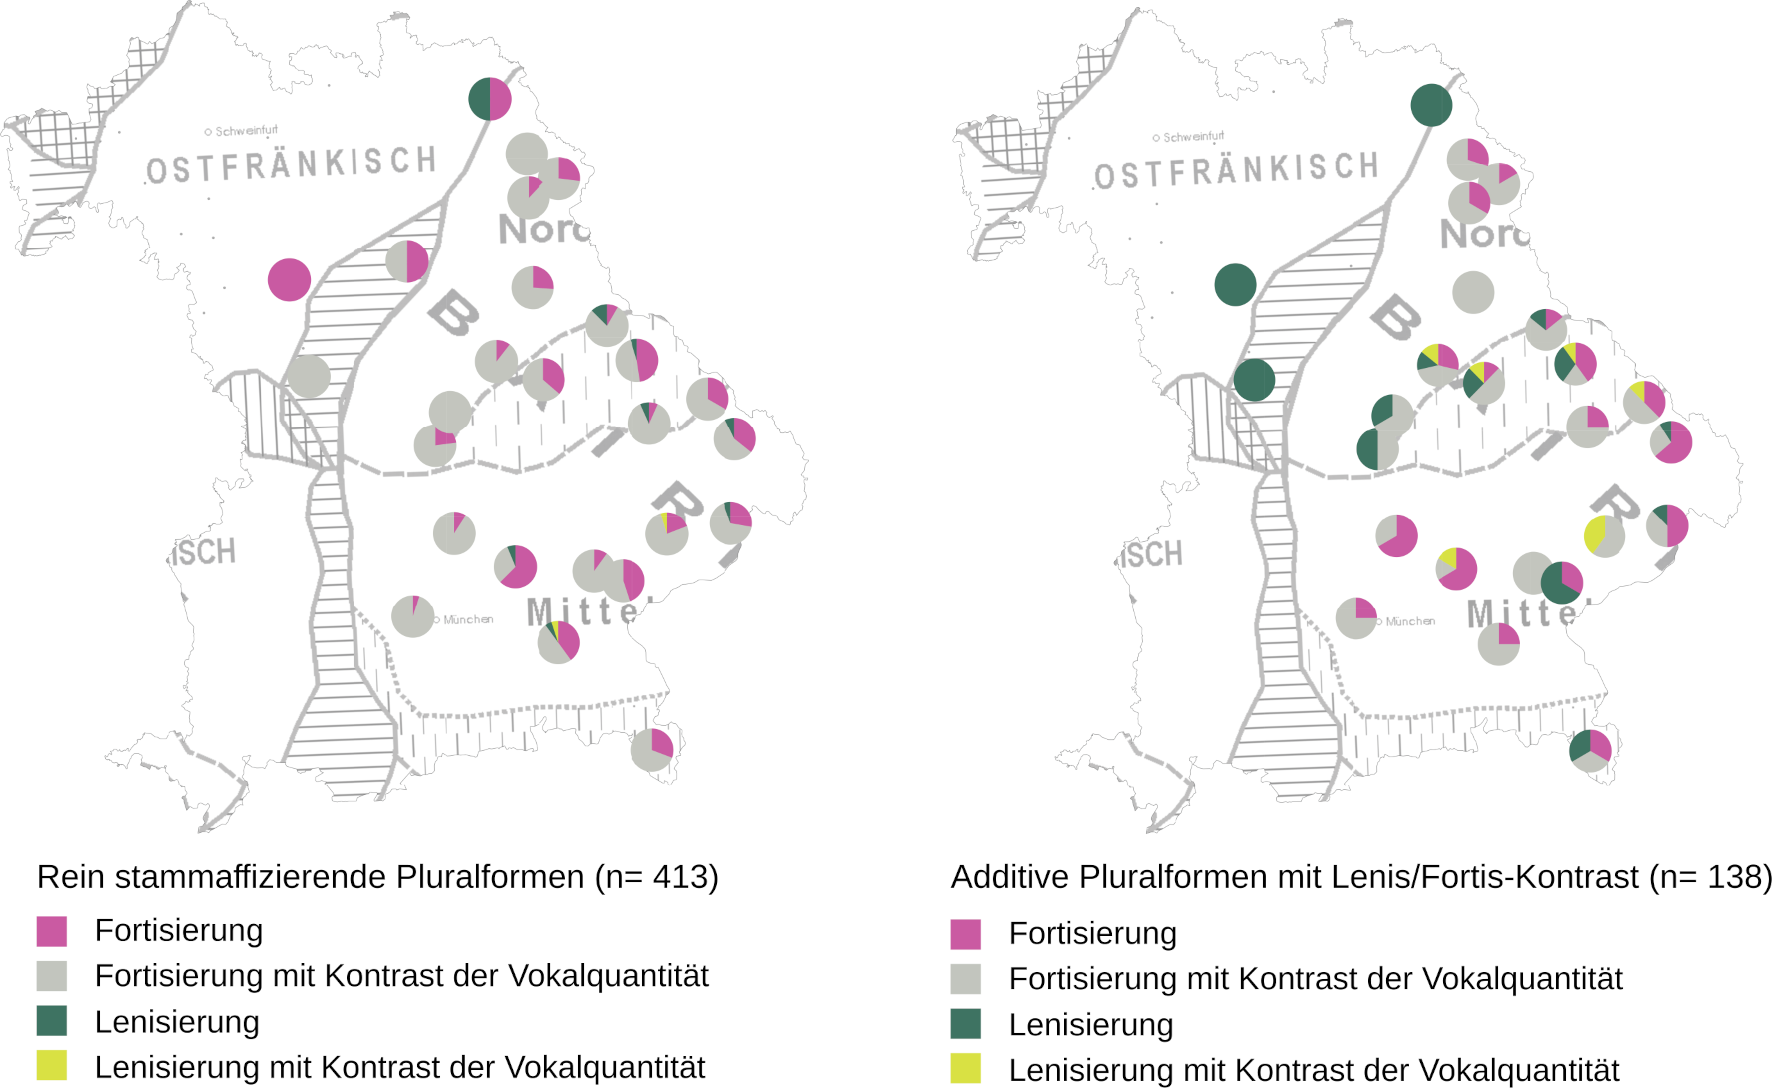
\includegraphics[width=\textwidth]{figures/Karte12.png}
\caption{Häufigkeitsverteilung innerparadigmatischer Lenis-Fortis-Kontraste im In- und Auslaut bei stammaffizierenden und additiven Pluralformen ($n=551$)}
\label{map:12}
\end{map}
\vfill\pagebreak

Tatsächlich zeigt die Gegenüberstellung von additiven und stammaffizierenden Verfahren, dass bei additiven Formen der Anteil an Lenes im Plural größer ist als in stammaffizierenden Pluralformen. Insbesondere im nordbair.-mittelbair. Übergangsgebiet, teilweise auch im Mittelbair. wird der Stammauslaut vor Nasalsuffix regelmäßig lenisiert (z.\,B. \teuthoo{An}{αn} \teuthoo{imp,\_}{imp͓ʰ} -- \teuthoo{imbqm}{imbʔm} ‚Imme‘ im nordbair.-mittelbair. Blaibach, \teuthoo{mu94<k,\_}{mu\klammeruntenpost{}̣̂k͓ʰ} -- \teuthoo{mu94<gán@}{mu\klammeruntenpost{}̣̂ɡ͈n̥} ‚Mücke‘ im mittelbair. Reischach). In einem Viertel der Lenisierungen entspricht die Korrelation von Vokal- und Konsonantismusquantität dabei dem bair. Silbengesetz, im Singular erscheint Kurzvokal+Fortis und im Plural Langvokal+Lenis, z.\,B. \teuthoo{A}{α} \teuthoo{tSe.3k}{tʃĕͅk} -- \teuthoo{tSe:<gn@}{tʃê{\doubleogonek}ɡn̥} ‚Zecke‘ im nordbair.-mittelbair. Blaibach. Insgesamt kann hier aber allenfalls von Tendenzen gesprochen werden, da sich für additive Pluralformen mit Nasalsuffix gleichermaßen Belege für Lenis im Singular und Fortis im Plural finden: \teuthoo{do<x1d}{dôx\⚬d} -- \teuthoo{do<x1t,n@}{dôx\⚬t͓n̥} ‚Docht‘ (ohne Quantitätskontrast) im nordbair.-mittelbair. Blaibach, \teuthoo{ho.<us\%}{hôͅus͈} -- \teuthoo{ho.uS,n@}{hoͅuʃ͓n̥} ‚Hase‘ (mit Quantitätskontrast) im mittelbair. Neukirchen am Inn. Daneben bietet \citet[§61.6]{Schießl1914} einen Hinweis darauf, dass die Lenis-Fortis-Alternation auch phonotaktisch bedingt sein kann: Im mittelbair. Dialekt von Eichendorf erscheint Fortis in der Verbindung Na\-sal+Den\-tal\-plo\-siv+Na\-sal „ausnahmslos“, das heißt, in additiven Pluralformen des Typs \textit{šd\~und} -- \textit{šd\~untn} ‚Stunde‘ oder in schwachen Akkusativ-Singular-Formen wie \textit{bl\~{\i}nd} -- \textit{ən bl\~{\i}ntn} ‚einen Blinden‘ ist Fortisplosiv durch die phonologische Umgebung gesteuert.

Auch bei den apokopierten Singularstammformen finden sich verschiedene Realisierungen der Vokal- und Konsonantenquantitätsverhältnisse und der Alternationsmuster, wie \tabref{tab:27} exemplarisch für drei Feminina im nordbair.-mittelbair. Übergangsgebiet illustriert: Während es für \textit{Brücke} und \textit{Straße}\footnote{Nach \citet[1093]{Wiesinger1983e} sind mhd. Langvokale wie mhd. \textit{â} in \textit{Straße} vor Frikativ- und Plosivgeminaten im Mittel- und Nordbair. sowie im Unterofr. regulär gekürzt worden.}  zum Teil innerparadigmatische Fortis/Lenis-Alternationen (teilweise auch in Korrelation mit der Vokalquantität) vor Nasalsuffix gibt, findet sich für \textit{Achse} kein innerparadigmatischer Wechsel. Interessant ist in diesem Zusammenhang außerdem, dass apokopierte Singularformen nur in der Tendenz, nicht aber grundsätzlich, Fortisauslaut aufweisen (dies modelliert die Tiefenstruktur /aksa/ vs. [aks] ‚Achse‘ nach \citealt[44]{Hinderling1980}), und sich verschiedene (Gegen-)Beispiele mit Konsonantismusalternation finden, z.\,B. \teuthoo{se).Nsd}{se\klammeruntenpost{}ͅŋsd} -- \teuthoo{se).Nst,-n@}{se\klammeruntenpost{}ͅŋst͓{}͐n̥} ‚Sense‘ im nordbair. Windischeschenbach und \teuthoo{bi.Agá\_}{biͅαɡ͈ʰ} -- \teuthoo{bi.AkAn}{biͅαkαn} ‚Birke‘ im mittelbair. Kirchensur.


\begin{table}
\begin{tabular}{lllll}
\lsptoprule
& {Singular} & {Plural} & {Diminutiv} & \\
\midrule
 ‚Achse‘ & \teuthoo{dqa4k,S}{dʔạk͓ʃ} & \teuthoo{dqa4kSn@}{dʔạkʃn̥} &  & Bernhardswald\\
& \teuthoo{a4<gðs5}{ậɡ̩s̩} & \teuthoo{a4<gðs5n@}{ậɡ̩s̩n̥} &  & Bernried\\
& \teuthoo{a4ks}{ạks} & \teuthoo{a4ksn@}{ạksn̥} &  & Blaibach\\
& \teuthoo{wo4<Na4kS}{wộŋạkʃ} & \teuthoo{wo4<Na4kSn@A}{wộŋạkʃn̥α} &  & Grafenkirchen\\
& \teuthoo{a4k,S,}{ạk͓ʃ͓} & \teuthoo{a4kSn@}{ạkʃn̥} &  & Zwiesel\\
\tablevspace
 ‚Brücke‘ & \teuthoo{bru.k,\_}{bruͅk͓ʰ} & \teuthoo{bru.gðn@}{bruͅɡ̩n̥} & \teuthoo{brigðl°@}{briɡ̩l̥̑} & Bernhardswald\\
& \teuthoo{brugá}{bruɡ͈} & \teuthoo{brugáAn}{bruɡ͈αn} & \teuthoo{brI.?gáAl}{brı̈ͅɡ͈αl} & Bernried\\
& \teuthoo{bru4k\_}{brụkʰ} & \teuthoo{bru.gðn@}{bruͅɡ̩n̥} & \teuthoo{bri4gðe4}{brịɡ̩ẹ} & Blaibach\\
& \teuthoo{bruk\_}{brukʰ} & \teuthoo{bru.kN@}{bruͅkŋ̥} & \teuthoo{brikl}{brikl} & Grafenkirchen\\
& \teuthoo{bruk\_}{brukʰ} & \teuthoo{bruk,An}{bruk͓αn} & \teuthoo{brI.?kAl}{brı̈ͅkαl} & Zwiesel\\
\tablevspace
 ‚Straße‘ & \teuthoo{s\#dra.S}{šdraͅʃ} & \teuthoo{s\#dra.2sn@}{šdrāͅsn̥} & \teuthoo{s\#dra4Sl.@}{šdrạʃl̥ͅ} & Bernhardswald\\
& \teuthoo{s\#5d5roS}{š̩d̩roʃ} & \teuthoo{s\#5d5ra4Sn@}{š̩d̩rạʃn̥} & \teuthoo{s\#5d5ra4SAl}{š̩d̩rạʃαl} & Bernried\\
& \teuthoo{s\#dra.S}{šdraͅʃ} & \teuthoo{s\#dra.Sn@}{šdraͅʃn̥} & \teuthoo{s\#dra4Sl@}{šdrạʃl̥} & Blaibach\\
& \teuthoo{s\#dra.S}{šdraͅʃ} & \teuthoo{s\#dra.Sn@}{šdraͅʃn̥} & \teuthoo{s\#dra4Sý@}{šdrạʃɫ̥} & Grafenkirchen\\
& \teuthoo{s\#d5ra:S}{šd̩ra{\doubleogonek}ʃ} & \teuthoo{s\#5d5ra.2sn@}{š̩d̩rāͅsn̥} & \teuthoo{s\#5d5ra4<s\%l@}{š̩d̩rậs͈l̥} & Zwiesel\\
\lspbottomrule
\end{tabular}
\caption{Exemplarische Beispiele apokopierter Singularformen -- Plural mit Nasalsuffix im nordbair.-mittelbair. Übergangsgebiet\label{tab:27}}
\end{table}

So heterogen das bisherige Bild bei CVC(C)-Einsilbern ist, so heterogen sind auch die Quantitätsverhältnisse bei zweisilbigen CVCV-Sequenzen, d.\,h. bei historischen Mehrsilbern. Auch hier findet sich vereinzelt ein Nebeneinander von Lenis- und Fortisalternanzen, z.\,B. \teuthoo{o):kA}{o\klammeruntenpost{}{\doubleogonek}kα} -- \teuthoo{a4gáA}{ạɡ͈α} ‚Acker‘ im nordbair.-mittelbair. Bernried vs. \teuthoo{o<.gáA}{ôͅɡ͈α} -- \teuthoo{a4<k,A}{ậk͓α} (neben \teuthoo{a4<gáA}{ậɡ͈α}) im mittelbair. Neukirchen am Inn, daneben gibt es vereinzelte Beispiele für Lenisierungen wie \teuthoo{ha4f,A}{hạf͓α} -- \teuthoo{ha4v\%An}{hạv͈αn} -- Dim. \teuthoo{ha4i.v\%e4}{hạiͅv͈ẹ} ‚Hafen‘ im mittelbair. Grafenau. Die Gegenüberstellung von exemplarischen Zweisilbern in den mittelbair. Tiefenbohrungspunkten (\tabref{tab:28}) zeigen einerseits, dass es Belege für die Kombination von Langvokal+Fortiskonsonanz (bei \textit{Mutter}) und von Kurz\-vo\-kal+Le\-nis\-kon\-so\-nanz (\textit{Apfel} in Inning am Holz und Neukirchen) in den Daten gibt (vgl. \citealt{MoosmüllerBrandstätter2014}). Anderseits gibt es Variation im Singularparadigma hinsichtlich der Vokalquantität (vgl. Nom. und Dat.Sg. von \textit{Mutter} in mittelbair. Kirchensur und Pasing) sowie zwischen Nom.Sg., Nom.Pl. bzw. Diminutivform hinsichtlich Lenis-Fortis-Konsonanz (vgl. \textit{Schwester} im mittelbair. Inning am Holz und Neukirchen sowie \textit{Apfel} in Inning am Holz).

\begin{table}[p]
\begin{tabularx}{\textwidth}{llQQl}
\lsptoprule
& {Nom.Sg.} & {Nom.Pl.} & {Dat.Sg.} & \\
\midrule
 ‚Mutter‘ & \teuthoo{b-mu.<AtE}{b{}͐mûͅαtə} & \teuthoo{b-mîiAtE@}{b{}͐m{\aufstrih}iαtə̥} &  & Inning am Holz\\
& \teuthoo{b5muAtA}{b̩muαtα} & \teuthoo{muAtAn}{muαtαn} & \teuthoo{A}{α} \teuthoo{dA}{dα} \teuthoo{mu<AtA}{mûαtα} & Kirchensur\\
& \teuthoo{b-mu.<AtE}{b{}͐mûͅαtə} & \teuthoo{mu94<AtEn}{mu\klammeruntenpost{}̣̂αtən} & \teuthoo{dA4mu4<AtEn}{dα̣mụ̂αtən} & Neukirchen am Inn\\
& \teuthoo{b\_mu.<AtA}{bʰmûͅαtα} & \teuthoo{mu.AtAn}{muͅαtαn} & \teuthoo{A}{α} \teuthoo{dA}{dα} \teuthoo{mu.<AtAn}{mûͅαtαn} & Niedertaufkirchen\\
& \teuthoo{b5\_mu.AtA}{b̩ʰmuͅαtα} & \teuthoo{miAtA}{miαtα} & \teuthoo{dA}{dα} \teuthoo{mu.<AtA}{mûͅαtα} & Pasing\\
& \teuthoo{b5mu.AtA}{b̩muͅαtα} & \teuthoo{bmi.AtA}{bmiͅαtα} & \teuthoo{dA}{dα} \teuthoo{muAtA}{muαtα} & Wolfersdorf\\
\tablevspace
 ‚Schwester‘ & \teuthoo{mâa4<e+}{m{\aufstrih}ậẽ} \teuthoo{s\#wes\%t,A4}{šwes͈t͓α̣} & \teuthoo{ma4<i.ne}{mậiͅne} \teuthoo{s\#we4S,t;An}{šwẹʃ͓t͓͓αn} &  & Inning am Holz\\
& \teuthoo{ma4<e<}{mậê} \teuthoo{s\#we4Sd5A}{šwẹʃd̩α} & \teuthoo{ma4<e<ne4}{mậênẹ} \teuthoo{s\#we4Sd5An}{šwẹʃd̩αn} &  & Kirchensur\\
& \teuthoo{ma4i:}{mai{\doubleogonek}} \teuthoo{s\#wes\%d\%A}{šwes͈d͈α} & \teuthoo{ma4<i.ne}{mậiͅne} \teuthoo{s\#wes\%t;En}{šwes͈t͓͓ən} &  & Neukirchen am Inn\\
& \teuthoo{ma4<e4}{mậẹ} \teuthoo{s\#we4s5t,A}{šwẹs̩t͓α} & \teuthoo{ma4e4ne4}{mạẹnẹ} \teuthoo{s\#we4s5tAn}{šwẹs̩tαn} &  & Niedertaufkirchen\\
& \teuthoo{m{\textasciitilde}ôe.<I:}{m{\aufstrih}êi{\doubleogonek}} \teuthoo{s\#we4Sd\%A}{šwẹʃd͈α} & \teuthoo{m{\textasciitilde}ôe.>(+i:(6nîi:}{m{\aufstrih}êi{\doubleogonek}n{\aufstrih}i{\doubleogonek}}
 \teuthoo{s\#we4Sd\%An}{šwẹʃd͈αn} &  & Pasing\\
& \teuthoo{mâa4>(+e>(+}{m{\aufstrih}ậ̃\klammerobenpost{}ễ\klammerobenpost{}} \teuthoo{s\#we4Sd5A}{šwẹʃd̩α} & \teuthoo{ma4+e+ne4}{mạ̃ẽnẹ} \teuthoo{{s\#we4Sd5A}n}{šwẹʃd̩αn} &  & Wolfersdorf\\
\midrule & Nom.Sg. & Nom.Pl. & Diminutiv & \\\midrule
 ‚Apfel‘ & \teuthoo{o4b5v\%e}{ọb̩v͈e} & \teuthoo{e4<b5v\%e}{ệb̩v͈e} & \teuthoo{e4b\%fAl}{ẹb͈fαl} & Inning am Holz\\
& \teuthoo{o4pfe4}{ọpfẹ} & \teuthoo{e4pfe4}{ẹpfẹ} & \teuthoo{a4pfAl}{ạpfαl} & Kirchensur\\
& \teuthoo{ob5v\%e}{ob̩v͈e} & \teuthoo{e94bv\%e?}{e\klammeruntenpost{}̣bv͈ë} & \teuthoo{a4b\%v\%Al}{ạb͈v͈αl} & Neukirchen am Inn\\
& \teuthoo{o4pfe4}{ọpfẹ} & \teuthoo{e4pfe4}{ẹpfẹ} & \teuthoo{a4pfAl}{ạpfαl} & Niedertaufkirchen\\
& \teuthoo{a.pfîi:}{aͅpf{\aufstrih}i{\doubleogonek}} & \teuthoo{e4pfîi:}{ẹpf{\aufstrih}i{\doubleogonek}} & \teuthoo{a4pfAl°}{ạpfαl̑} & Pasing\\
& \teuthoo{a:pfe4}{a{\doubleogonek}pfẹ} & \teuthoo{e4pfe4}{ẹpfẹ} & \teuthoo{a4pfAl}{ạpfαl} & Wolfersdorf\\
\lspbottomrule
\end{tabularx}
\caption{Quantitätsverhältnisse in CVCV-Strukturen in den mittelbair. Tiefenbohrungspunkten (Auswahl)\label{tab:28}}
\end{table}

Anhand dieses exemplarischen Blicks in die BSA-Daten wird deutlich, dass für die Analyse -- neben der (morpho)phonologischen Ebene -- notwendigerweise die Ebene der Transkription berücksichtigt werden muss. Teilweise bestehen die Lenis-Fortis-Kontraste in nur einem Segment einer Konsonantensequenz, teilweise nur in der Abstufung der Diakritika, vgl. \teuthoo{no.2Xd}{nōͅꭗd} -- \teuthoo{na4x5d\%}{nạx̩d͈} ‚Nacht‘ im mittelbair. Pasing (vgl. die Typisierungsprinzipien in \sectref{sec:6.3.1.2}).\footnote{\citet[13]{Schießl1909} zeigt der in seiner phonetischen Darstellung des mittelbair. Dialekts von Eichendorf, dass Lenis-Fortis-Kontraste bei Velarfrikativ [x] durch die weniger starke „Reibeenge“ weniger deutlich ausfallen als bei den übrigen Frikativen oder bei Plosiv, demnach können zudem unterschiedlich starke Kontraste für die einzelnen konsonantischen Artikulationsarten angenommen werden.} Artikulation findet eben nicht in Form binärer phonologischer Oppositionen, sondern als Ausprägungen einer kontinuierlichen Skala statt; die Teuthonista als sehr fein abgestuftes Transkriptionssystem dokumentiert diese z.\,T. minimalen phonetischen Unterschiede. So sieht auch \citet[22]{Scheutz1984} als Ergebnis seiner Quantitätsmessungen „die eher kontinuierliche als streng dichotomische Skalierung der Quantitätsverhältnisse“ als „ein kaum zu leugnendes Faktum“ an. Dies wurde auch während der Exploration des \textit{Bayerischen Sprachatlas} beobachtet, wie ein Blick in den Einführungsband des SNiB zeigt:

\begin{quote}
Insgesamt wurde im Erhebungszeitraum außerdem festgestellt, dass die Bestimmung der Vokalquantitäten, vor allem vor Frikativ oder Nasalkonsonant oft sehr schwierig ist. Der damit in Zusammenhang stehende Gegensatz von Lenis-Fortis ist oft nicht eindeutig. Die tatsächliche Realisierung verstößt häufig gegen die ‚bairische Gesetzmäßigkeit‘ von Fortes nach Kurzvokal, Lenes nach Langvokal und Diphthongen. (\citealt[23]{SNiB1})\footnote{Vgl. auch \citet[405--406]{Götz1987} zu Schwierigkeiten der Transkription der bair. Quantitätsverhältnisse.}
\end{quote}

Eine Auswertung von innerparadigmatischen Quantitätskontrasten in den Daten des BSA kann nicht losgelöst von methodischen Spezifika der BSA-Daten stattfinden, die morphophonologische Analyse ist zunächst immer an die phonetische Ebene gekoppelt. Darüber hinaus ist die Lenis-Fortis-Alternation aus morphophonologischer Sicht auch deshalb besonders interessant, weil sie im Mittelbair. „gewissermaßen ein Doppelleben“ \citep[191]{Seiler2008} führt: Sie ist sowohl morpho(phono)logisch als auch phonologisch konditioniert, selbst wenn entsprechende Lenis-Fortis-Alternationen synchron lexikalisiert und nicht das Ergebnis eines produktiven phonologischen Prozesses sein sollten (vgl. \citealt[19]{Scheutz1984}).

\subsubsubsubsection{Lenis-Fortis-Kontraste zwischen Lexikalisierung und Produktivität}


Das hohe Maß an phonetischer Variation, die sich für die bair. Daten insgesamt und auch innerhalb der einzelnen Tiefenbohrungspunkte zeigt (vgl. die vorgestellten instrumentalphonetischen Studien sowie die exemplarischen Beispiele in 	\tabref{tab:28}), hat wiederum Auswirkungen auf die Modellierung als morphophonologisches Verfahren. Die Analyse der BSA-Daten zeigt hier, in welchem Maße Morphologie an Phonetik und Phonologie gebunden ist, und wie Sprecher des Bair. (morpho)phonologische Oppositionen als Pluralmarkierungsstrategien nutzen. So finden sich in den Daten Belege, dass Lenis-Fortis-Kontraste im UG als Pluralmarkierungsstrategie (teilweise in Kombination mit Kontrasten der Vokalquantität) im bair. Teil des UGs morphologisiert sind. \tabref{tab:29} zeigt zunächst innerparadigmatische Alternationen bei zweisilbigen CVCV-Segmenten auf.


\begin{table}
\begin{tabularx}{\textwidth}{lllQ}
\lsptoprule
{Singular} & {Plural} & {Diminutiv} & \\
\midrule
 \teuthoo{o4<b5v5l°@}{ộb̩v̩l̥̑} & \teuthoo{epfl°@n@}{epf‌l̥̑n̥} &  & ‚Apfel‘ (nordbair.-mittelbair. Bernhardswald)\\
 \tablevspace
 \teuthoo{goAd\%-n@}{ɡoαd͈n̥} & \teuthoo{ga4rt-n@}{ɡạrt͐n̥} & \teuthoo{ga4rtl@}{ɡạrtl̥} & ‚Garten‘ (nordbair.-mittelbair. Zwiesel)\\
 \tablevspace
 \teuthoo{ha4<gðl@}{hậɡ̩l̥} & \teuthoo{ha4k;l@n}{hạk͓͓l̥n} & \teuthoo{ha4<gAl}{hậɡαl} & ‚Haken‘ (mittelbair. Neukirchen am Inn) \\
 \tablevspace
 \teuthoo{mu<g-N@}{mûɡ{}͐ŋ̥} & \teuthoo{muk-N@}{muk{}͐ŋ̥} &  & ‚Mücke‘ (mittelbair. Grafenau)\\
 \tablevspace
 \teuthoo{bmu<EdA}{bmûədα} & \teuthoo{mutEn}{mutən} &  & ‚Mutter‘ (nordbair.-mittelbair. Grafenkirchen)\\
 \tablevspace
 \teuthoo{o4<v\%A}{ộv͈α} & \teuthoo{e4<f;A}{ệf͓͓α} &  & ‚Ofen‘ (nordbair. Oberdolling)\\
 \tablevspace
 \teuthoo{s\#u.b\%v\%A}{šuͅb͈v͈α} & \teuthoo{d5s\#5u.pfAn}{d̩š̩uͅpfαn} &  & ‚Schupfen‘ (mittelbair. Grafenau)\\
 \tablevspace
 \teuthoo{do94Xd\%A}{do\klammeruntenpost{}̣ꭗd͈α} & \teuthoo{d5e.Xt,A4}{d̩eͅꭗt͓α̣} &  & ‚Tochter‘ (mittelbair. Inning am Holz)\\
 \tablevspace
 \teuthoo{wu.(<Ed5s5ý@}{wûͅ\klammerobenpost{}əd̩s̩ɫ̥} & \teuthoo{wi.Et,S,ý@}{wiͅət͓ʃ͓ɫ̥} &  & ‚Wurzel‘ (nordbair. Groschlattengrün)\\
\lspbottomrule
\end{tabularx}
\caption{Lenis-Fortis-Kontraste in CVCV-Strukturen}
\label{tab:29}
\end{table}

Belege wie diese finden sich in vorhandenen Dialektdarstellungen kaum (vgl. \textit{Schindel} -- \textit{Schindtl} ‚Schindel‘ für das nordbair. Muttersdorf bei \citealt{Micko1933}, zitiert nach \citealt[123]{Rowley1997}). \citet[123]{Rowley1997} etwa kann in seinen nordostbayerischen Daten keine Belege für eine Morphologisierung des Lenis-Fortis-Kontrasts finden. Und auch in den vorliegenden Daten handelt es sich um einzelne Belege dieser Pluralmarkierungsstrategie für die jeweiligen Lexeme,\footnote{Für \textit{Mutter} ist in Blaibach und Bernhardswald (nordbair.-mittelbair. Übergangsgebiet) Lenisierung belegt: \teuthoo{bmuAtA}{bmuαtα} -- \teuthoo{muAdAnA}{muαdαnα} (Blaibach), \teuthoo{muEt,E}{muət͓ə} -- \teuthoo{mu<EdAnE}{mûədαnə} (Bernhardswald).} sodass sich nicht sagen lässt, ob es sich um lexikalisierte Formen handelt oder ob die Gewährspersonen sie spontan in Form von kumulierten Markierungsstrategien realisierten. (Nur im Fall von \teuthoo{mu<g-N@}{mûɡ{}͐ŋ̥} -- \teuthoo{muk-N@}{muk{}͐ŋ̥} ‚Mücke‘ im mittelbair. Grafenau besteht der formale Unterschied einzig im Quantitätenkontrast, die Alternative wäre damit Nullplural.)

Neben den Lenis-Fortis-Alternationen bei zweisilbigen CVCV-Stämmen gibt es in den Daten Belege eines morphologisierten Verfahrens für historische Einsilber. Die Wechsel sind insofern „unvoraussagbar“ \citep[46]{Hinderling1980}, als sie (in der Terminologie Hinderlings) historische „Lenislexeme“ betreffen, für die die Alternation nicht infolge eines (diachronen oder synchronen) phonetisch-phonologischen Prozesses entstanden ist, z.\,B. -- bei historischem Langvokal -- \teuthoo{ma<os}{mâos} -- \teuthoo{ma<iS}{mâiʃ} (nordbair. Tirschenreuth) und \teuthoo{ma(<4u.s5}{mâ\klammerobenpost{}̣uͅs̩} -- \teuthoo{ma43i.S}{mặiͅʃ} ‚Maus‘ (nordbair. Windischeschenbach).\footnote{\citet[329]{Zehetner1983} zählt für den Freisinger Stadtdialekt synchron auch \textit{Hut} zu den Lenisstämmen, da die Leniskonsonanz auch in anderen Stammformen erhalten ist, \textit{Huad} -- \textit{Hiad} neben Dim. \textit{Hiadal}. Folgt man dieser synchronen Klassifikation, gibt es in den vorliegenden Daten auch für diesen Lenisstamm analoge Lenis-Fortis-Kontraste im Nordbair. und nordbair.-mittelbair. Übergangsgebiet, z.\,B. \teuthoo{hôo.ud}{h{\aufstrih}oͅud} -- \teuthoo{hôe.it}{h{\aufstrih}eͅit} (nordbair. Nabburg).} Für die Alternation bei \textit{Maus} finden sich in den SNOB-Roh\-da\-ten weitere Belege im nördlichen Nordbair., sodass die kumulierte Pluralmarkierungsstrategie in diesem Gebiet tatsächlich lexikalisiert zu sein scheint (vgl.  \mapref{map:9} zu Quantitätskontrasten altem Langvokal oder Diphthong).


\begin{map}
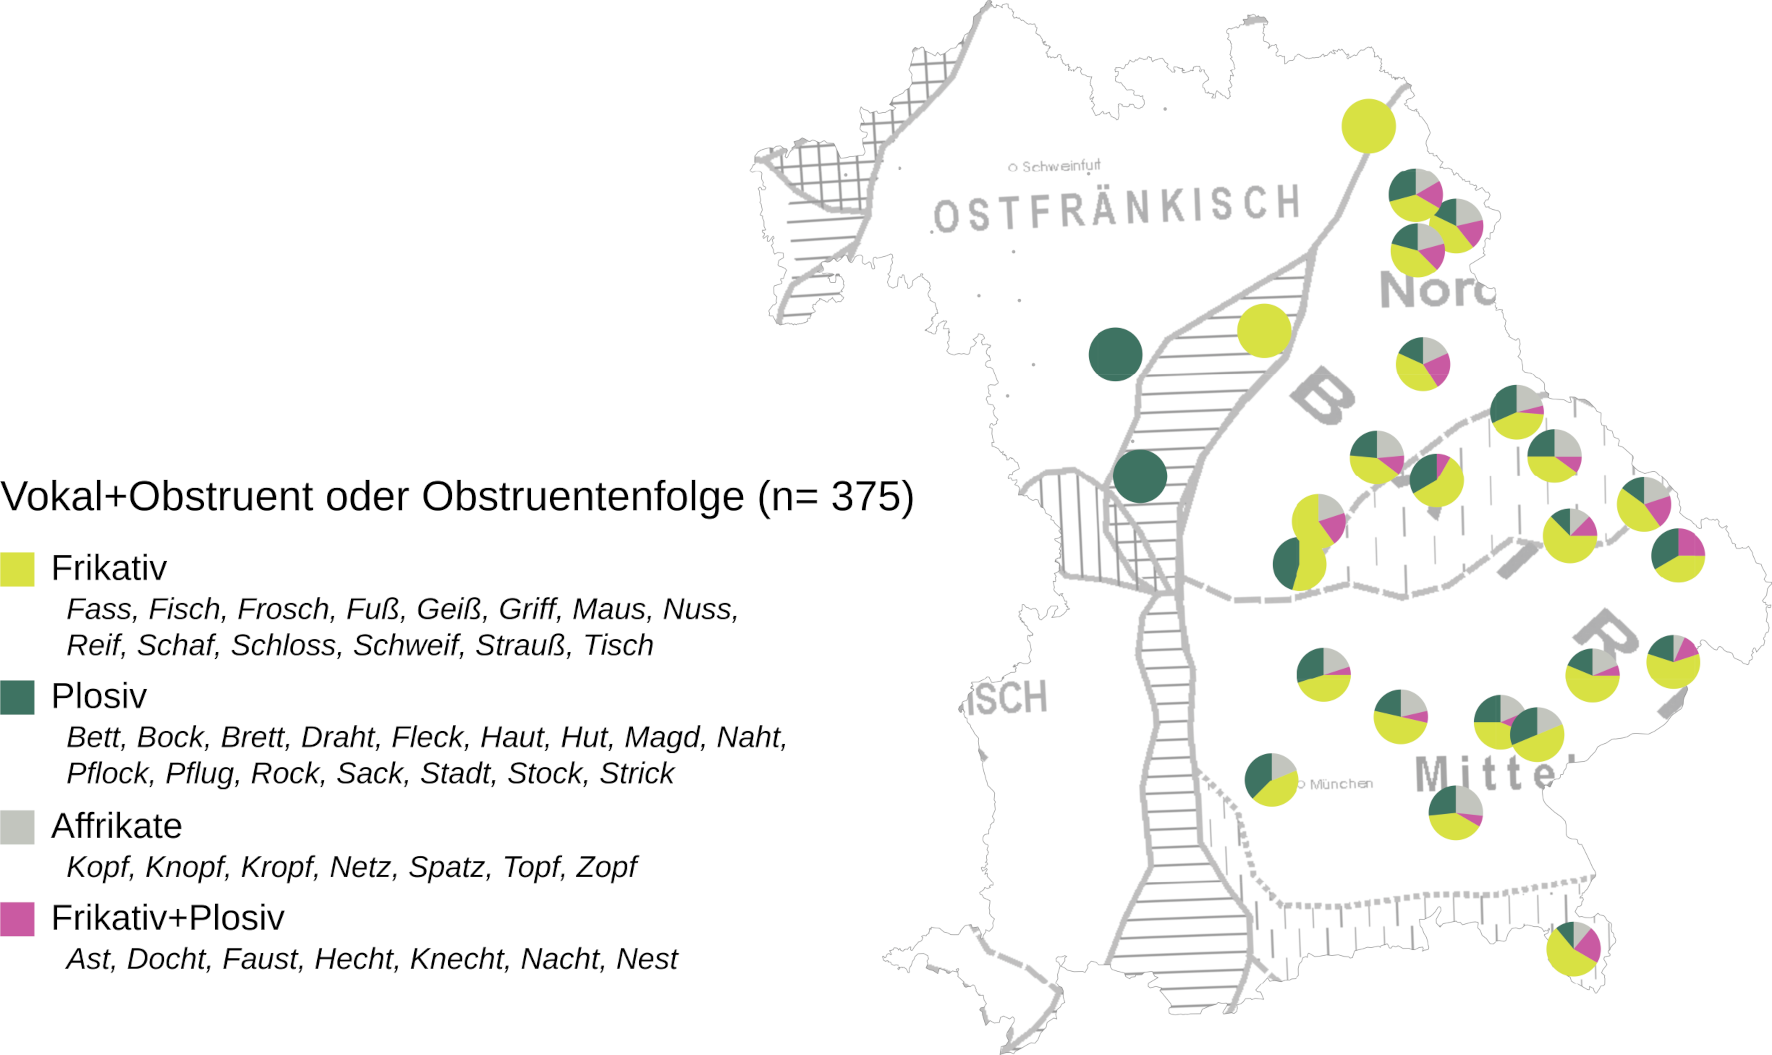
\includegraphics[width=\textwidth]{figures/Karte13.png}
\caption{Lenis-Fortis-Kontraste in Einsilbern in verschiedenen phonologischen Umgebungen}
\label{map:13}
\end{map}

Eine differenzierte Analyse von Leniskonsonanz im Singular und Fortiskonsonanz im Plural bei historischen Einsilbern zeigt darüber hinaus, dass die innerparadigmatische Alternation (respektive deren Fehlen) durch die Konsonanz (Einzelkonsonant oder Konsonantenfolge) des Auslauts bedingt sein kann (\mapref{map:13}). Lenis-Fortis-Kontraste finden sich in den verschiedenen (teilweise auch allen) phonologischen Umgebungen in den nördlichen nordbair. Tiefenbohrungspunkten. Die mittelbair. Ortspunkte und jene des nordbair.-mittelbair. Übergangsgebietes weisen insgesamt größere Unterschiede auf, da die innerparadigmatische Alternation hier nicht für sämtliche Konsonantenarten oder bei Konsonantenverbindungen belegt ist.\footnote{So finden sich beispielsweise im nordbair. Riedenburg keine Alternationen bei Plosiven, in verschiedenen mittelbair. Tiefenbohrungspunkten finden sich keine Belege für Alternationen bei Dental- oder Velarplosiv. Vereinzelt weisen Tiefenbohrungspunkte Alternation für Konsonantenfolgen, aber keine Alternation bei Affrikaten auf (mittelbair. Grafenau, nordbair.-mittelbair. Bernhardswald). Bemerkenswert ist, dass im nordbair. Oberdolling systematisch keine Lenis-Fortis-Kontraste bei Konsonantenfolgen erscheinen, bei Einzelkonsonanten aber sämtliche Obstruenten belegt sind.}

Auf der Lexemebene sind bei Einsilbern mit Vokal-Obstruent-Abfolge regionale Schwankungen zu beobachten, die v.\,a. durch lexemspezifische Entwicklungen bedingt sind. Einzelne Lexeme haben großräumige Geltung, andere sind nur in einem kleineren Gebiet oder vereinzelt belegt:

\begin{itemize}\sloppy
\item Bei den Frikativen sind großräumig \textit{Schweif}, \textit{Reif}, \textit{Griff}; \textit{Fuß}, \textit{Geiß}, \textit{Schloss} und \textit{Fisch}, \textit{Frosch}, \textit{Tisch} belegt, im Nordbair. finden sich daneben \textit{Fass}, \textit{Strauß}.
\item Lenis-Fortis-Kontrast bei Plosiv findet sich großräumig für \textit{Haut}, \textit{Sack}, \textit{Stock}, \textit{Rock}, vereinzelt im Nordbair und im nordbair.-mittelbair. Übergangsgebiet \textit{Bett}, \textit{Hut} und \textit{Stadt}.
\item Lenis-Fortis-Kontraste in wortfinalen Konsonantenclustern haben für die Abfolge /st/ in \textit{Ast}, \textit{Faust} großräumige Geltung (vereinzelt findet sich \textit{Fest}). /xt/ ist im Nordbair. teilweise belegt für \textit{Docht} und \textit{Hecht} und im gesamten bair. UG vereinzelt bei \textit{Nacht} und \textit{Knecht} (vgl. \citealt[33]{Hinderling1980}, \citealt[119]{Seiler2005}).\footnote{In Liquid-Obstruent-Abfolgen, die hier nicht kartiert wurden, finden sich vereinzelt Fortisierungen bei \textit{Bild}, \textit{Feld}, \textit{Holz} und \textit{Wald} im Nordbair. Großräumig im Nord- und Mittelbair. finden sich Lenis-Fortis-Kontraste in /r/-Obstruent-Abfolgen bei \textit{Dorf}, vereinzelt bei \textit{Wirt}, \textit{Markt}, \textit{Korb}, \textit{Herz} (jeweils mit vokalisiertem /r/).}
\item Die Affrikaten /pf/ und /ts/ sind großräumig für \textit{Knopf}, \textit{Kropf}, \textit{Zopf} und vereinzelt \textit{Topf} und \textit{Netz} im Nordbair. bzw. nordbair.-mittelbair. Übergangsgebiet belegt.
\end{itemize}

Systematisch neutralisiert ist nach \citet[45]{Zehetner1978} „die Wirkkraft“ des sogenannten Bair. Silbengesetzes in Abfolgen aus /r/+Obstruent und auch bei Nasal+Obstruent, es finden sich Kombinationen von Kurzvokal und Leniskonsonanz (vgl. \citealt{Hinderling1980}: 28). Laut \citet[123]{Rowley1997} besteht im südlichen Nordbair. der formale Unterschied zwischen Singular- und Pluralform in Nasal-Obstruent-Abfolgen einzig im Lenis-Fortis-Kontrast. Dieser Befund findet sich in den vorliegenden Daten in einzelnen Ortsdialekten des Nord- und Mittelbair. wieder: Im mittelbair. Kirchensur und im nordbair. Tirschenreuth gibt es keine Belege für Vokalquantitätskontraste vor Nasal+Obstruent in historischen Einsilbern, daneben werden auch in anderen mittelbair. und teilweise nordbair. Tiefenbohrungspunkten innerparadigmatische Kontraste vor Nasal+Obstruent nur in Form von Lenis-Fortis-Kontrasten realisiert, z.\,B. \teuthoo{s\#wa.nds5}{šwaͅnds̩} -- \teuthoo{s\#wa4ntS}{šwạntʃ} ,‚Schwanz‘ (mittelbair. Kirchensur) und \teuthoo{A}{α} \teuthoo{hund}{hund} -- \teuthoo{hunt\_}{huntʰ} -- Dim. \teuthoo{hund5Al}{hund̩αl} ‚Hund‘ (nordbair.-mittelbair. Blaibach). Insgesamt scheint es sich aber v.\,a. um lexemspezifische Entwicklungen zu handeln. So sind \textit{Hund} und \textit{Strumpf} ohne Quantitätskontraste in Ortspunkten belegt, die Quantitätskontraste bei anderen Lexemen (z.\,B. \textit{Schwanz} und \textit{Band}) aufweisen.

Damit zeigt die Auswertung der einzelnen Obstruenten und Konsonantenabfolgen im Auslaut der Singularform, dass die phonologische Umgebung eine Variable ist, die für jeden Ortsdialekt bedingt, ob innerparadigmatische Quantitätskontraste (von Vokal und/oder Obstruent) im System des Ortsdialekts als Pluralmarkierungsstrategie zur Verfügung stehen. Daneben scheint die Art des Kodierungsverfahrens häufig lexemspezifisch zu sein.


\begin{figure}
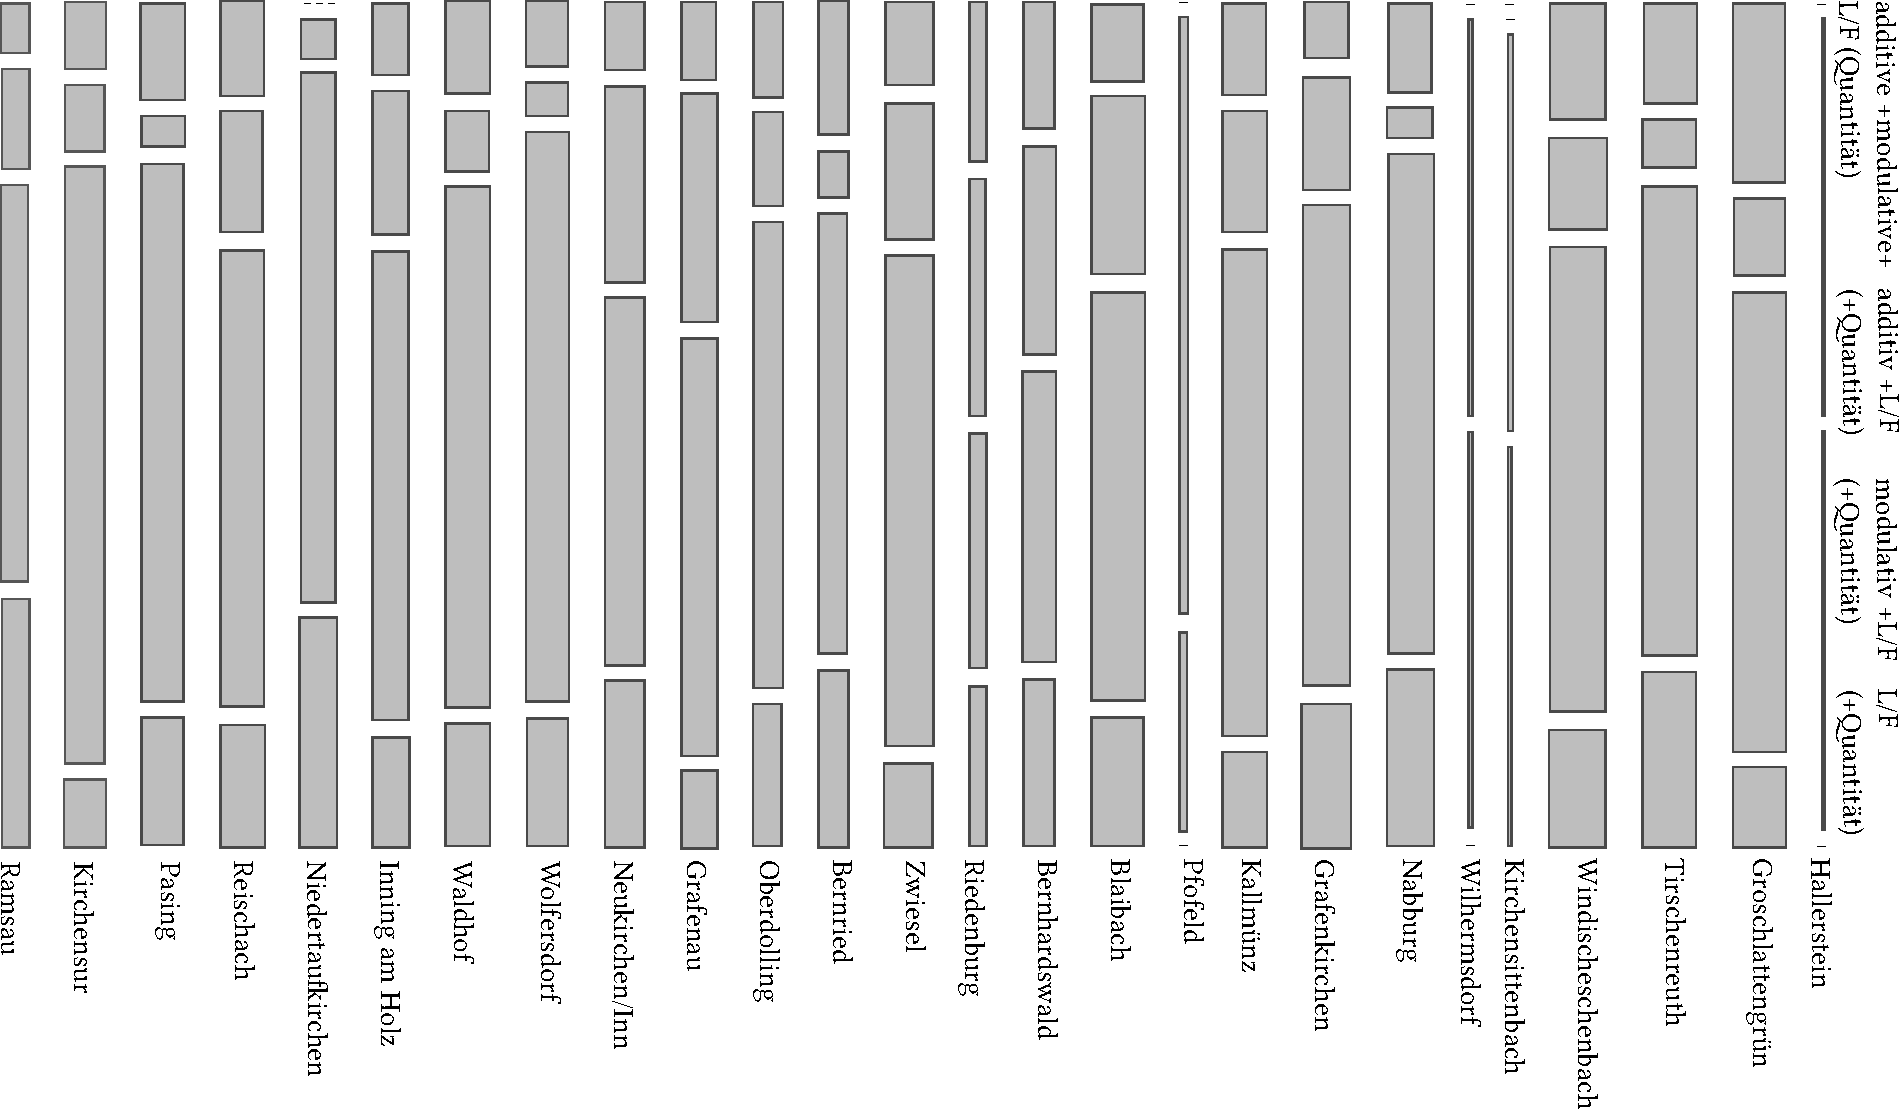
\includegraphics[height=0.75\textwidth, angle=90]{figures/revisedNickelNominalmorphologie-img022.pdf}
\caption{Mosaik-Plot mit Häufigkeitsverteilung von Lenis-Fortis-Kontrasten (L/F) in Kombination mit anderen additiven und stammaffizierenden Verfahren ($n=508$)}
\label{fig:6}
\end{figure}

Lenis-Fortis-Kontraste erscheinen als kumulative Pluralmarkierungen vor allem in Kombination mit Kontrasten der Vokalqualität als weiterem stammaffizierenden Verfahren, wie das Mosaik-Plot in  \figref{fig:6} für alle Tiefenbohrungspunkte mit Lenis-Fortis-Kontrasten illustriert. Das Mosaik-Plot visualisiert die Variablen Ortsdialekt (von Nord nach Süd), Typus des Pluralverfahrens und absolute Häufigkeit. Anhand der Größe der Flächen der Rechtecke ergibt sich, dass die Vorkommenshäufigkeit in den Dialekten schwankt, in den ofr. Ortsdialekten handelt es sich um ein nur peripheres Phänomen. Das Plot zeigt zudem, dass die relative Häufigkeit von Lenis-Fortis-Kontrasten in Kombination mit einem additiven Verfahren in den einzelnen Ortsdialekten z.\,T. stark schwankt, es überwiegen Kombination aus additiv-modulativer Markierung und Quantitätskontrasten. Innerhalb des Nord- und Mittelbair. scheint es hier ortsdialektspezifische Präferenzen zu geben, in welchem Umfang und in welcher Kombination innerparadigmatische Lenis-Fortis-Kontraste als Kodierungsverfahren im Flexionssystem den Sprechern zur Verfügung stehen.

An dieser Stelle ist eine Vorausschau auf Genus als möglichem Konditionierungsfaktor der Deklinationsklassenzugehörigkeit sinnvoll, da die Unterschiede im Mosaik-Plot hinsichtlich der Präferenz einzelner Markierungsstrategien für die Ortsdialekte durch Genus bedingt sind (ausführlicher \sectref{sec:8.3.1}). \mapref{map:14} visualisiert für die areale Dimension die Häufigkeitsverteilung
von Lenis-Fortis-Kontrasten nach Genus differenziert. In allen Ortspunkten sind innerparadigmatische Lenis-Fortis-Kontraste am häufigsten für Maskulina belegt. Dieser Typus von Konsonantismusalternationen ist in den rezenten Dialekten in der Tendenz ein spezifisch maskulines Verfahren, was primär durch die historische Deklinationsklassenzugehörigkeit bedingt ist (vgl. \sectref{sec:8.2.1}). Unterschiede zwischen den Ortspunkten ergeben sich v.\,a. durch unterschiedliche Anteile von Feminina und Neutra. Das mittelbair. Grafenau etwa sticht mit einem vergleichsweise hohen Anteil an Feminina heraus. Der Blick in die Daten zeigt, dass hier Lenis-Fortis-Kontraste nicht nur bei Feminina der historischen \textit{i}{}-Deklination belegt sind, sondern auch in CVCV-Strukturen produktiv ist (z.\,B. \teuthoo{mu<g-N@}{mûɡ{}͐ŋ̥} -- \teuthoo{muk-N@}{muk{}͐ŋ̥} ‚Mücke‘, vgl. 	\tabref{tab:29}).

\begin{map}[p]
\centering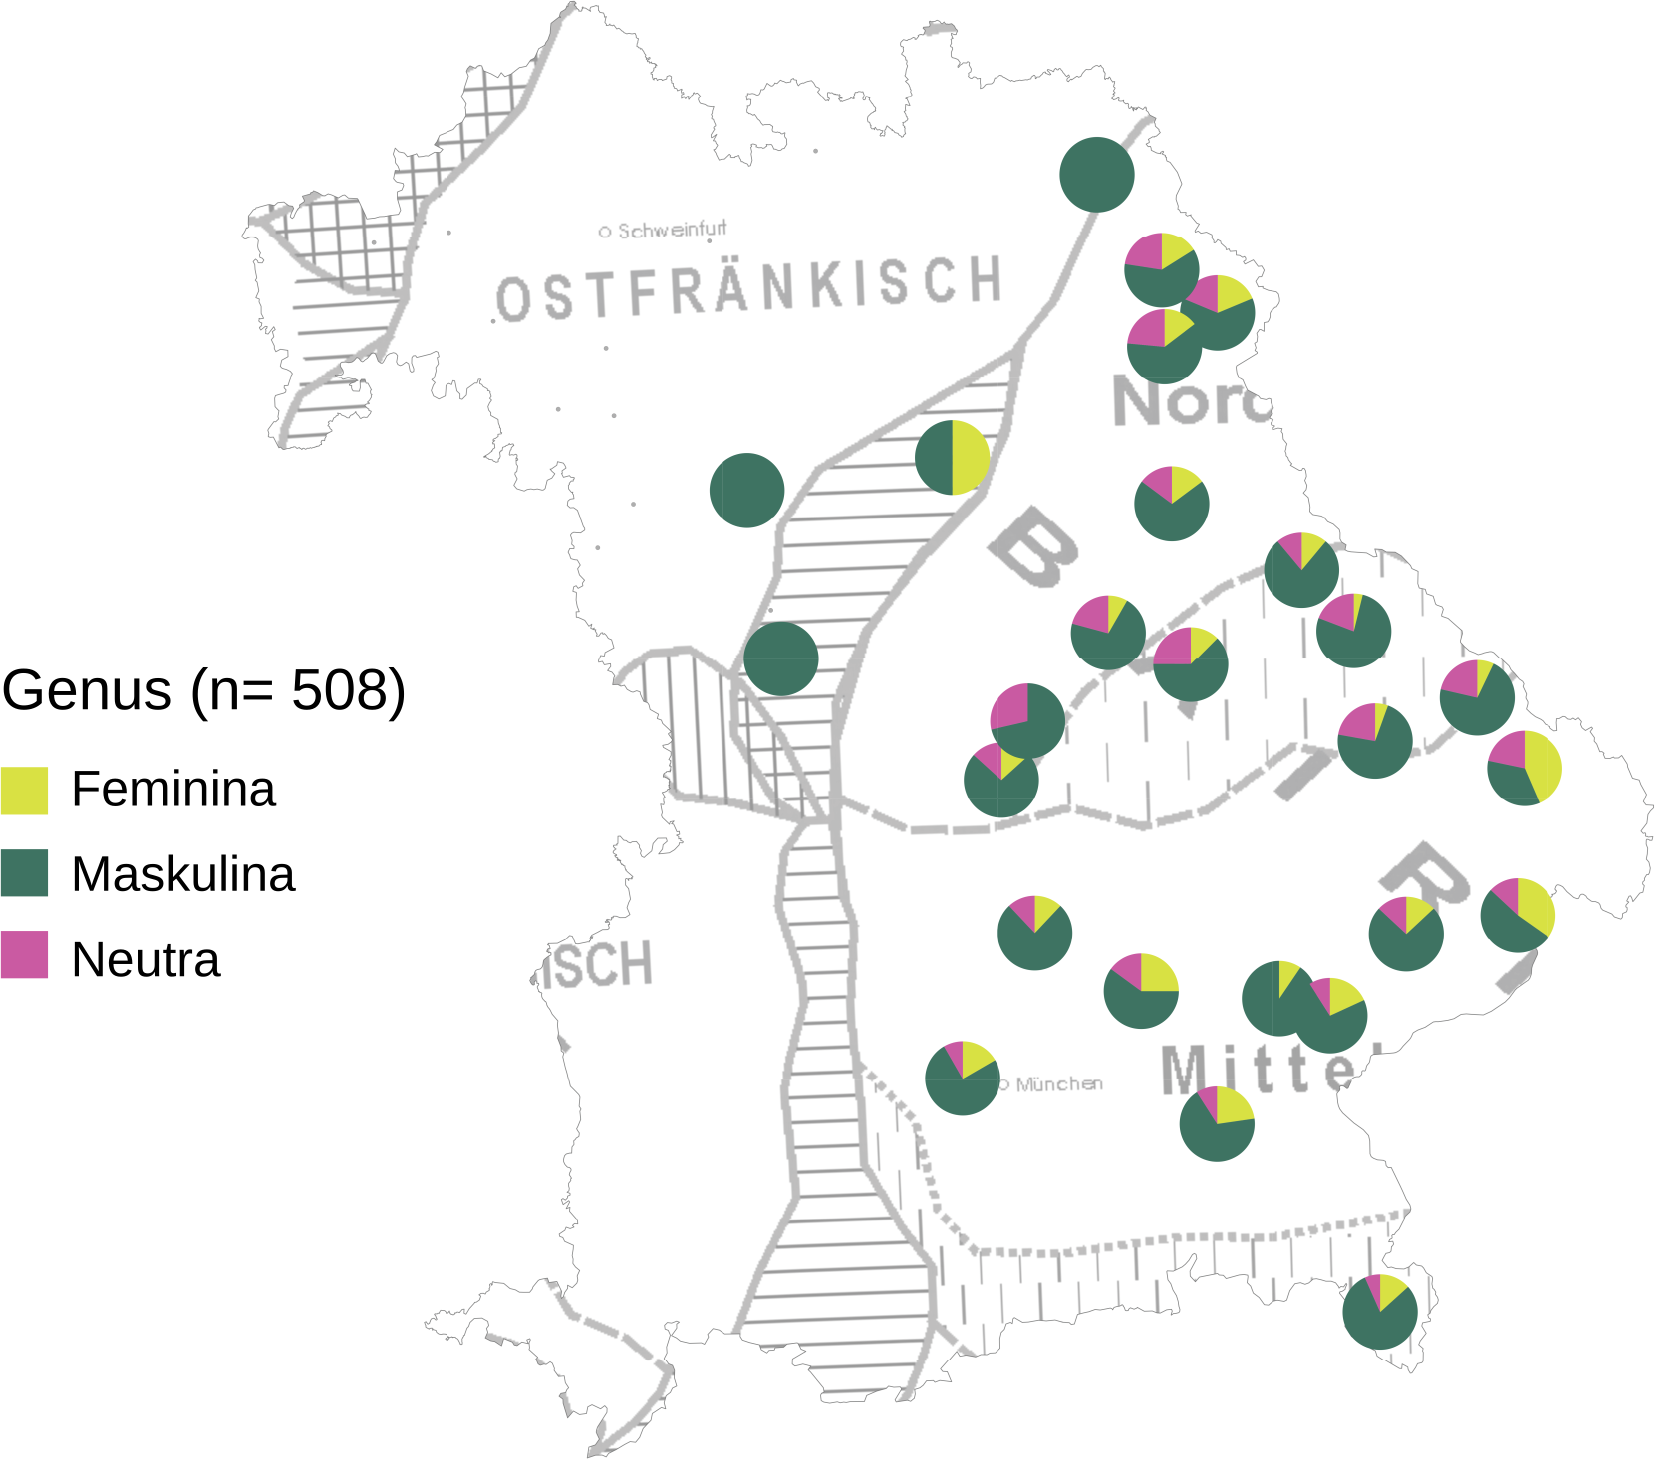
\includegraphics[width=.8\textwidth]{figures/Karte14.png}
\caption{Häufigkeitsverteilung der Lenis-Fortis-Kontraste für die Genera}
\label{map:14}
\end{map}

\begin{table}[p]
\begin{tabular}{lrrr}
\lsptoprule
     &  Maskulinum & Femininum & Neutrum\\
     \midrule
     add/kons/quant & 6 & 16 & 25\\
     add/mod/kons/quant & 4 & 2 & 54\\
     kons/quant & 79 & 9 & 0\\
     mod/kons/quant & 260 & 53 & 0\\
     \lspbottomrule
\end{tabular}
\caption{Korrespondenzanalyse der Variablen Genus und Pluralmarkierungsverfahren ($n=507$)}
\label{tabfig:7}
\end{table}


Dass die Wahl des Kodierungsverfahrens primär durch Genus konditioniert ist, illustriert auch die Korrespondenzanalyse in  \figref{fig:7} und \tabref{tabfig:7}.\footnote{Diese und folgende Korrespondenzanalysen wurden erstellt mit dem R-Paket \textit{languageR} von Harald Baayen (vgl. \citealt{Baayen2015}, \url{https://www.rdocumentation.org/packages/languageR}).} Diese Art der multivariaten Analyse ermöglicht „a low-dimensional map of the data“ \citep[129]{Baayen2015}, in diesem Fall unter Vernachlässigung der arealen Dimension. Analysiert werden die absoluten Werte einer zweidimensionalen Kreuztabelle, wobei zunächst zwei Abstandsmatrizen mittels Chi-Quadrat-Distanz berechnet werden (eine Matrix für den Abstand zwischen den Spalten und eine Matrix für den Abstand zwischen den Zeilen, vgl. \citealt[129--136]{Baayen2015}). In einem zweiten Schritt werden die Abstände dann als Streuungsdiagramm in einem orthogonalen Koordinatensystem visualisiert. Je größer die Abstände zwischen Zeilen und Spalten sind, desto größer sind auch die Abstände im Plot. Die Koordinatenachsen des Plots werden durch zwei Merkmale, hier Genus und Kodierungsverfahren, gebildet, die einzelnen Datenpunkte sind durch die Labels der verschiedenen Merkmalsausprägungen dargestellt. Fälle mit ähnlicher Merkmalsausprägung erscheinen im Plot gruppiert, sodass sich für die Variablen Genus und Art des kombinierten Kodierungsverfahrens durch ihre relative Entfernung zueinander sagen lässt, dass rein stammaffizierende Verfahren dialektunabhängig ein Verfahren der Maskulina sind, während additiv-modulative Markierung mit Lenis-Fortis-Kontrasten häufiger mit Neutrum (Typ \teuthoo{vo2s}{vōs} -- \teuthoo{va4SA}{vạʃα} ‚Fass‘) und additive Markierung mit Lenis-Fortis-Kontrasten eher mit Femininum korrelieren, in geringerem Maße aber auch mit Neutrum (Typ \teuthoo{ne2sd}{nēsd} -- \teuthoo{neStA}{neʃtα} ‚Nest‘).

\begin{figure}[h]
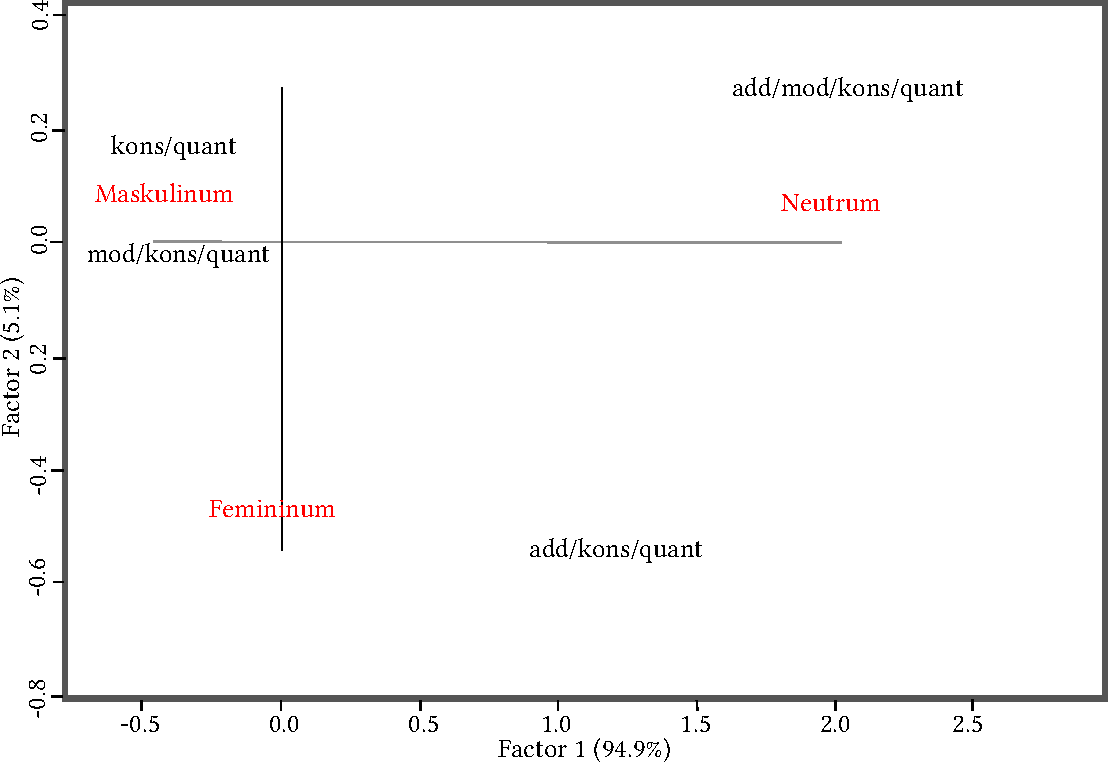
\includegraphics[width=\textwidth]{figures/revisedNickelNominalmorphologie-img024.pdf}
\caption{Korrespondenzanalyse der Variablen Genus und Pluralmarkierungsverfahren ($n=507$)}
\label{fig:7}
\end{figure}

Zusammenfassend lässt sich sagen, dass synchrone Lenis-Fortis-Alternationen (meist in Kombination mit Kontrasten der Vokalquantität) mehrheitlich durch diachronen phonologischen Wandel und damit lautgesetzlich entstanden sind. Darüber hinaus finden sich einzelne Beispiele für analoge Lenis-Fortis-Kontraste, sodass von einem funktionalisierten und zumindest teilweise produktiven Ko"-die"-rungs"-ver"-fah"-ren ausgegangen werden kann. Gleichzeitig zeigen die Daten, dass Lenis-Fortis-Kontraste nicht nur ein „Doppelleben“ \citep{Seiler2008} zwischen Phonologie und Morphologie führen, sondern dass auch Variation in der Artikulation, d.\,h. auf der phonetischen Ebene, vorhanden ist. Diese Variation besteht einerseits diachron in Form von Dialektwandel für dieses Dialektmerkmal (vgl. die vorgestellten instrumentalphonetischen Studien), und auch synchron spiegeln die BSA-Daten wider, dass Quantitätskontraste weniger binär sind, sondern innerhalb eines phonetischen Kontinuums stattfinden. Der entscheidende Punkt ist demnach weniger das Doppelleben zwischen Phonologie und Morphologie, sondern vielmehr das Doppelleben, das Lenis-Fortis-Kontraste als Kodierungsverfahren und im Sprachgebrauch der einzelnen Sprecher führen:\footnote{Vgl. hierzu \citegen[84--85]{Seiler2018} Überlegungen zu Chomskys Konzept I(nternal)- vs. E(xternal)-language.} In welchem Maße tolerieren Sprecher und Hörer des Nord- und Mittelbair. Schwankungen und eventuelle Uneindeutigkeiten der Vokal- und Konsonantenquantität, solange der Kontext die Numerusinformation disambiguiert?\footnote{Ambig sind Formen derweil nur, wenn Pluralmarkierung nur durch Lenis-Fortis-Kontraste und nicht in Form eines kombinierten Verfahrens erfolgt.}  In welchen Kontexten wird die Variation in der sprecherseitigen Realisierung vereindeutigt? Aus flexionsmorphologischer Perspektive schließt sich folgende Frage an: Wieviel Variation „verträgt“ ein Pluralmarkierungsverfahren? Anhand des untersuchten Materials (insbesondere im Hinblick auf Transkriptionseffekte) kann nicht abschließend geklärt werden, wo die Grenzen der Variation für dieses stammaffizierende Markierungsverfahren liegen. Und für die flexionsmorphologische Klassifikation stellt sich schließlich die Frage, in welchem Maße Quantitätskontraste überhaupt eine eigene Deklinationsklasse konstituieren können, wenn sie so anfällig für phonetische Variation sind (siehe \sectref{sec:8.1}).

Mit Blick auf den Sprachgebrauch ist Variation bei der Realisierung der Lenis-Fortis-Opposition einerseits auf der Produktions- und Perzeptionsebene anzusiedeln (nämlich zwischen Sprach\-ökonomie und Explizitheit der Markierung flexivischer Information, vgl. \citealt[88]{Seiler2018}, ausführlicher hierzu \sectref{sec:10.3}). Ein weiterer Aspekt von Variation kann durch das Sprachsystem lizensiert sein. \citet[124]{Steininger1994} beschreibt die Möglichkeit fakultativer Pluralmarkierung bei Lenis-Fortis-Kontrasten im Dialekt Oberneureutherwaids. Wie auch beim potenzierten Plural nach \textit{n}{}-Erweiterung im Singular der Feminina (Typ \teuthoo{das\#n}{dašn} -- \teuthoo{das\#nA}{dašnα} ‚Tasche‘) werden die Quantitätskontraste zur Disambiguierung genutzt. Ist der Plural bereits durch ein Zahlwort markiert, erfolgt keine innerparadigmatische Alternation; Leniskonsonanz ist dann auch in der Pluralform im Auslaut möglich: \textit{d̥iːʒ} -- \textit{d̥iʃ} ‚Tisch‘, aber \textit{t̥sβæ d̥i:ʒ} ‚zwei Tische‘ (\citealt[124]{Steininger1994}, vgl. \sectref{sec:9.2}). Gleichzeitig findet tatsächlich ein Wandel in der Pluralmarkierung statt, wie \citet{Wildfeuer2001} in seinem Apparent-time-Vergleich dreier Altersgruppen nachweist. Im mittelbair. Dialekt von Kirchdorf findet ein Abbau der Pluralmarkierung mittels Quantitäts- und Lenis-Fortis-Kontrast für das Lexem \textit{Tisch} statt. Ca. 70\,\% bzw. 80\,\% der Gewährspersonen der beiden älteren Sprechergruppen bilden den Plural nach diesem Muster, während in der jüngeren Sprechergruppe die Mehrzahl (60\,\%) den Plural nicht markiert (Nullplural gegenüber 40\,\% mit Kontrast der Vokalquantität und Lenis/Fortis, vgl. \citealt[189--190]{Wildfeuer2001}).

\subsubsubsection{Konsonantenelision -- 0/K- vs. K/0-Alternationen}\label{sec:7.1.2.3.2}\largerpage
Eine zweite Form der Pluralmarkierung mittels Konsonantismuskontrast besteht im gesamten UG in der innerparadigmatischen Alternation zwischen Formen mit elidiertem vs. erhaltenem Konsonanten. Die Beispiele in \tabref{tab:30} belegen verschiedene Muster der Konsonantenelision. In der Singularform ist der auslautende Plosiv oder Nasal jeweils elidiert, in allen drei Diminutivformen dagegen erhalten.\footnote{Die Diminutivformen werden hier (wo möglich) vergleichend herangezogen, da der auslautende Nasal oder Obstruent vor dem Diminutivsuffix erhalten ist. Die Berücksichtigung von Diminutiven hat aus Perspektive der Formenbildung den Vorteil, dass Diminutivbildungen ein hohes Maß an formaler Regelmäßigkeit aufweisen (vgl. \citealt[110]{Rowley1997}). Hinzu kommt mit Blick auf die Datenlage, dass sie als einziger Wortbildungstypus sehr regelmäßig und im gesamten UG in den BSA-Erhebungen abgefragt wurden.} Für die Pluralformen können nun drei Muster unterschieden werden, die als zwei unterschiedliche Wechseltypen klassifiziert werden.


\begin{table}
\begin{tabular}{llll}
\lsptoprule
{Singular} & {Plural} & {Diminutiv} & \\
\midrule
 \teuthoo{bu2E}{būə} & \teuthoo{bu2E\textbf{w}E}{būə\textbf{w}ə}
 & \teuthoo{bu"?E\textbf{w}lE}{bǖə\textbf{w}lə} & ‚Bube‘ (Gemünden am Main)\\
 \teuthoo{s\#lo24}{šlọ̄} & \teuthoo{s\#la24g}{šlạ̄\textbf{g}} & \teuthoo{s\#la24\textbf{g}Al}{šlạ̄\textbf{g}αl} & ‚Schlag‘ (Blaibach)\\
 \teuthoo{dso"+}{dsȭ} & \teuthoo{dse"+}{dsẽ̄} & \teuthoo{dsa24\textbf{n}ErlA}{dsạ̄\textbf{n}ərlα}
 & ‚Zahn‘ (Nabburg) \\
\lspbottomrule
\end{tabular}
\caption{Konsonantenelision des Wechseltypus 0/K und 0/0}
\label{tab:30}
\end{table}

\begin{sloppypar}
In Singular-/Pluralformen des Typus \teuthoo{bu2E}{būə} -- \teuthoo{bu2EwE}{būəwə} ist der Konsonant als Stammauslaut im Singular elidiert, im Plural ist er im Inlaut vor dem Pluralsuffix erhalten; die Pluralmarkierung besteht damit in einer Kombination aus additivem und stammaffizierendem Verfahren. Die Pluralmarkierung des Typus \teuthoo{s\#lo24}{šlọ̄} -- \teuthoo{s\#la24g}{šlạ̄ɡ} hingegen ist rein stammaffizierend. Der im Singular elidierte Konsonant ist im Plural erhalten, sodass die Pluralform durch Modulation der Stammvokalqualität und innerparadigmatischer Konsonantismusalternation gebildet wird. Die beiden Typen \teuthoo{bu2E}{būə} -- \teuthoo{bu2EwE}{būəwə} und \teuthoo{s\#lo24}{šlọ̄} -- \teuthoo{s\#la24g}{šlạ̄ɡ} können hinsichtlich der Konsonantismusalternation und in Anlehnung an \citet[123--125]{Rowley1997} als Wechseltypus 0/K zusammengefasst werden: \textit{0} (d.\,h. Elision) im Singular, \textit{K} (d.\,h. Konsonant) im Plural.
\end{sloppypar}

Die Singular-/Pluralform des Typus \teuthoo{dso"+}{dsȭ} -- \teuthoo{dse"+}{dsẽ̄} entspricht einem zweiten Muster, dem Wechseltypus 0/0, d.\,h. hier ist der auslautende Konsonant im Singular und im Plural elidiert und nur in der Diminutivform erhalten. Erhalt vs. Elision des stammauslautenden Konsonanten kann lexemweise in den Ortsdialekten verschieden realisiert sein, wobei sich im gesamten UG die einzelnen Typen nachweisen lassen (daneben die Variante K/K mit erhaltenem Konsonant in beiden Formen, die im Folgenden der Vollständigkeit halber aufgeführt ist, vgl. 	\tabref{tab:31} exemplarisch für das Lexem \textit{Markt}). Welcher der Wechseltypen für ein Lexem realisiert wird, unterliegt arealen, z.\,T. recht kleinräumigen Schwankungen (vgl. \citealt[124]{Rowley1997}).


\begin{table}
\begin{tabularx}{\textwidth}{lQQ}
\lsptoprule
\makecell[tl]{{Konsonan-}\\{tismus}} & {Pluralmarkierungsverfahren} & {Ortsdialekte}\\
\midrule
K/K & \textit{Vokalqualität} \textit{(Umlaut)}

Typ \teuthoo{mo:rgd5}{mo{\doubleogonek}rɡd̩} -- \teuthoo{ma4rgd}{mạrɡd} (Wolfersdorf) & bair. Wolfersdorf, Zwiesel;

ofr. Hallerstein, Mitteleschenbach, Wiesthal\\
\tablevspace
& \textit{Vokalqualität} \textit{(Umlaut)} \textit{+} \textit{e}

Typ \teuthoo{moAkt\_}{moαktʰ} -- \teuthoo{meEkte\$}{meəkte̤} (Groschlattengrün) & bair. Grafenkirchen, Groschlattengrün, Oberdolling;

ofr. Gebsattel, Gemünden am Main, Krum\\
\tablevspace
& \textit{Null}

Typ \teuthoo{margd}{marɡd} -- \teuthoo{margd}{marɡd} (Hüttenheim) & bair. Kirchensur, Ramsau bei Berchtesgaden;

ofr. Hüttenheim\\
\tablevspace
0/0 & \textit{Vokalqualität} \textit{(Umlaut)}

Typ \teuthoo{ma.kH}{maͅkhͯ} -- \teuthoo{ma4kH}{mạkhͯ} (Waldhof) & mittelbair. Waldhof\\
\tablevspace
& \textit{Null}

Typ \teuthoo{moA4k\_}{moα̣kʰ} -- \teuthoo{moA4k\_}{moα̣kʰ} (Bernried) & bair. Bernried, Inning am Holz, Windischeschenbach;

ofr. Kirchensittenbach\\
\tablevspace
0/K & \textit{Vokalqualität} \textit{(Umlaut)}

Typ \teuthoo{A}{α} \teuthoo{mo.Ak,\_}{moͅαk͓ʰ} -- \teuthoo{ma4k,t,}{mạk͓t͓} (Bernhardswald) & bair. Bernhardswald, Kallmünz;

ofr. Pfofeld, Stadtschwarzach, Wilhermsdorf\\
\tablevspace
& \textit{Vokalqualität} \textit{(Umlaut)} \textit{+} \textit{e}

Typ \teuthoo{ma.rk}{maͅrk} -- \teuthoo{me.<rk,te4}{mêͅrk͓tẹ} (Niedertaufkirchen) & mittelbair. Niedertaufkirchen, Pasing, Reischach\\
\tablevspace
K/0 & \textit{Vokalqualität} \textit{(Umlaut)}

Typ \teuthoo{moAkt}{moαkt} -- \teuthoo{meEk}{meək} (Nabburg) & nordbair. Nabburg\\
\lspbottomrule
\end{tabularx}
\caption{Varianten der Konsonantismusalternation im UG für \textit{Markt}}
\label{tab:31}
\end{table}

\begin{sloppypar}
In \tabref{tab:31} ist ein vierter Wechseltypus (K/0) aufgeführt, bei dem der auslautende Konsonant in der Singularform erhalten, in der Pluralform hingegen elidiert ist. Die Struktur von Singular- und Pluralform dieses Wechseltypus gleicht einem subtraktiven Pluralmarkierungsverfahren: Der Stamm der Pluralform wird im Auslaut um ein Phonem reduziert (vgl. \citealt[582f.]{Dressler2000}, \citealt[25]{Birkenes2014} sowie \sectref{sec:7.1.2.4}). Die phonologischen Prozesse hinter dem K/0-Alternationsmuster sind sprachhistorisch jedoch von subtraktiver Morphologie zu unterscheiden, wie die folgenden Darstellungen zeigen werden.
\end{sloppypar}

Die Belege weiterer K/0-Alternationen in \tabref{tab:32} illustrieren, dass es sich im gesamten Korpus um ein eher peripheres Phänomen handelt, das ein Spezifikum des Bair., und zwar des Nordbair. zu sein scheint. Für die in 	\tabref{tab:32} aufgeführten Lexeme lassen sich im gesamten UG auch die übrigen Wechseltypen nachweisen. Die übergeordnete Frage lautet daher: Wie lassen sich die verschiedenen Fälle von innerparadigmatischer Alternation aus flexionsmorphologischer Perspektive systematisieren und modellieren? Stellt die innerparadigmatische Konsonantismusalternation durch Elision bzw. Erhalt des stammauslautenden Konsonanten ein eigenes Pluralmarkierungsverfahren dar (und inwiefern ist es als solches kognitiv verankert und überhaupt produktiv), inwiefern ist die innerparadigmatische Konsonantismusalternation aber auch nur eine phonetisch-phonologische „Begleiterscheinung“ der Pluralbildung?

\begin{table}[H]
\begin{tabular}{llll}
\lsptoprule
{Singular} & {Plural} & {Diminutiv} & \\
\midrule
\teuthoo{moAk\textbf{t}}{moαk\textbf{t}} & \teuthoo{meEk}{meək} &  & ‚Markt‘ (nordbair. Nabburg)\\
\teuthoo{ro2\textbf{d}}{rōi\textbf{d}} & \teuthoo{re42}{rẹ̄} & \teuthoo{ra42\textbf{d}l@}{rạ̄\textbf{d}l} & ‚Rad‘ (nordbair. Nabburg) \\
\teuthoo{lo<A\textbf{b}}{lôα\textbf{b}} & \teuthoo{lo2i}{lōi}. &  & ‚Laib‘ (nordbair. Windischeschenbach) \\
\teuthoo{mo2A\textbf{d}}{mōα\textbf{d}} & \teuthoo{mo9.2i}{mo\klammeruntenpost{}̄ͅi} &  & ‚Magd‘ (nordbair. Nabburg) \\
\teuthoo{tSa4o\$(+\textbf{n}}{tʃạõ\textbf{n}} & \teuthoo{t,S,ôo+i:6}{t͓ʃ{\aufstrih}õi{\doubleogonek}̃} &  & ‚Zaun‘ (mittelbair. Inning am Holz)\\
\lspbottomrule
\end{tabular}
\caption{Konsonantenelision des Wechseltypus K/0}
\label{tab:32}
\end{table}

Die Anzahl der Lexeme, die im Flexionsparadigma zwischen elidiertem vs. erhaltenem Konsonanten alternieren, ist im Korpus begrenzt und aufgrund der schwankenden regionalen Geltung „letztendlich Aufgabe der Ortsgrammatiken“ \citep[124]{Rowley1997}. Insgesamt handelt es sich um ein nicht allzu typenfrequentes Phänomen, das vor allem im Bair. zu einer spezifischen Formenbildung geführt hat. Da die Elision in- oder auslautender Obstruenten und Nasale auf unterschiedliche Regelmäßigkeiten und historische Entwicklungen zurückgeht, werden sie im Folgenden getrennt dargestellt.

\subsubsubsubsection{Elision von Obstruenten in Vokal-Konsonant-Abfolgen}

Der Schwund des Obstruenten in Vokal-Konsonant-Abfolgen und in der Finalposition in Konsonantenclustern ist diachron durch unterschiedliche phonologische Prozesse (Tilgung oder Assimilation an den vorausgehenden Konsonanten) entstanden. Da die innerparadigmatische Alternation zwischen erhaltenem vs. geschwundenem Konsonanten oder in Konsonantenclustern aus flexionsmorphologischer (und damit synchroner) Perspektive demselben Pluralmarker entspricht, werden die Phänomene im Folgenden gemeinsam behandelt.


\begin{map}
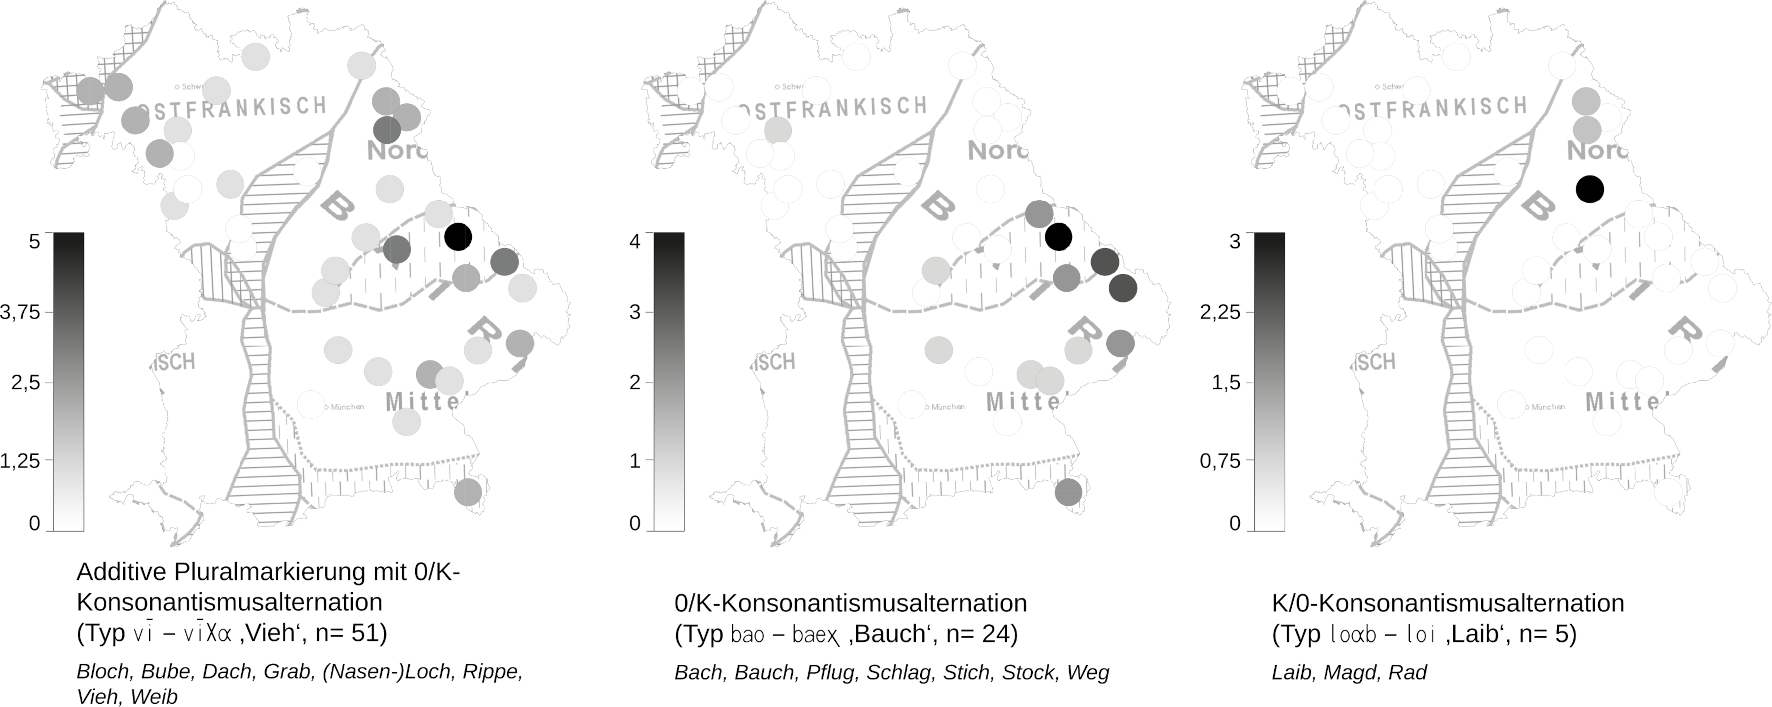
\includegraphics[width=\textwidth]{figures/Karte15.png}
\caption{Absolute Häufigkeit pro Ortsdialekt von innerparadigmatischer Alternation durch Konsonantenelision bei Vokal-Obstruent-Abfolge ($n=80$)}
\label{map:15}
\end{map}

\mapref{map:15} fasst die absolute Häufigkeit innerparadigmatischer Konsonantenelisionen im absoluten Auslaut bei Vokal-Obstruent-Abfolgen zusammen. Die Alternationen sind bei den einzelnen Lexemtypes im Korpus jeweils nur mit geringer Tokenanzahl belegt, insgesamt liegt eine z.\,T. recht kleinteilige, lexemspezifische areale Geltung vor. In Abhängigkeit von der konkreten Pluralmarkierungsstrategie können jedoch zwei Typen innerparadigmatischer Alternationen beschrieben werden: Wechsel zwischen elidiertem und erhaltenem Konsonanten (bzw. Konsonantenabfolge) in additiven Pluralformen (Typ \teuthoo{vi“}{vī} -- \teuthoo{vi“cA}{vīXα} ‚Vieh‘) und Wechsel zwischen elidiertem und erhaltenem Konsonanten in stammaffizierenden Pluralformen (Typ \teuthoo{bao}{bao} -- \teuthoo{baeX}{baeꭗ} ‚Bauch‘). Während Typ \teuthoo{vi“}{vī} -- \teuthoo{vi“cA}{vīXα} lexemweise im gesamten UG zu finden ist, stellen 0/K-Alternationen des Typs \teuthoo{bao}{bao} -- \teuthoo{baeX}{baeꭗ} ein -- wenn auch schwach besetztes -- spezifisch bair. Flexionsmuster dar.

Die Alternationen des Typs \teuthoo{bao}{bao} -- \teuthoo{baeX}{baeꭗ} sind das Ergebnis historischer phonologischer Prozesse, die Fortes und Lenes im In- und Auslaut im UG unterschiedlich affizierten.\footnote{Vgl. \citet[81--88]{Franke1895} zu einem Vergleich von Konsonantenelisionen im Ofr. und Obersächsischen (leider ohne Berücksichtigung der innerparadigmatischen Perspektive und möglicher Alternationen).} Im Zuge der sogenannten mittelbair. Konsonantenschwächung wurden die Fortisobstruenten ab ca. 1300 im Nord- und Mittelbair. lenisiert und sind z.\,T. mit den alten Lenes zusammengefallen.\footnote{Vgl. \citet[§34a und Karte 21]{Kranzmayer1956}, \citet[78--79]{Rowley1997}, \citet[271 und 302]{Schirmunski1962}.} Der bair. Dialektraum lässt sich infolge dieser Entwicklung in einen nord- und mittelbair. Teil gegenüber einem südbair. Teil mit erhaltenen Fortisobstruenten untergliedern, weshalb \citet[§34a2]{Kranzmayer1956} die Bedeutung der mittelbair. Konsonantenschwächung für das Bair. als „ebenso schwer“ wie die der hochdeutschen Lautverschiebung einordnet. Neben der nord- und mittelbair. Ausprägung des Lenisierungsprozesses greift im ofr. Teil des UGs die sogenannte binnenhochdeutsche Konsonantenschwächung, die sich z.\,T. auf das westliche Nordbair. ausdehnt (\tabref{tab:33}, vgl. \citealt[§34c1]{Kranzmayer1956}, \citealt[78]{Rowley1997}).

Aufgrund der phonologischen Prozesse Einsilberdehnung und mittelbair. Konsonantenschwächung (d.\,h. Lenisierung) bei gleichzeitig wirkendem bair. Silbengesetz kann für Einsilber mit historischem Fortisauslaut im Nord- und Mittelbair. von Leniskonsonanz im Auslaut ausgegangen werden (vgl. \citealt[28]{Grundler1951}). Hinzu kommt, dass in den Dialekten des UGs die Auslautverhärtung als Folge von Apokopierung und innerparadigmatischem Ausgleich im Singularparadigma früh zurückgenommen wurde, weshalb es, so \citet[78]{Rowley1997}, „zweckmäßig“ ist, auch bei Lexemen mit historischer Leniskonsonanz im Auslaut mhd. restituierte Lenes anzunehmen (vgl. \citealt[§27d]{Kranzmayer1956}).\largerpage[1.5]

Vor dem Hintergrund dieser historischen phonologischen Prozesse erklären sich nun die innerparadigmatischen Konsonantismusalternationen zwischen elidiertem vs. erhaltenem Obstruenten. Im primären und sekundären (d.\,h. durch Apokope entstandenen) Auslaut schwinden im Nordbair. um Cham und Teilen des Mittelbair. die mhd. restituierten Lenes \textit{b}, \textit{g}, teilweise \textit{d} sowie \textit{ch} in Einsilbern (\citealt[78]{Rowley1997}, \citealt[§28b2, 29c, 30b3, 33c]{Kranzmayer1956}). Dass rezente Konsonantismusalternationen bei Obstruenten im Kontext dieser historischen Prozesse und innerhalb des phonologischen Systems der nord- und mittelbair. Dialekte verstanden werden müssen, illustriert \citegen{Zehetner1978} Modellierung der Phoneme /b d g/ auf einem Spektrum phonetischer Realisierungen (\tabref{tab:34}).\pagebreak

\begin{table}[p]
\small
\begin{tabularx}{\textwidth}{>{\raggedright\arraybackslash}p{.17\textwidth}QQQ}
\lsptoprule
& Anlaut & Inlaut & Auslaut\\
\midrule
\multirow[2]{2}{=}{Binnen\-hoch\-deu\-tsche Kon\-so\-nan\-ten\-schwä\-chung} & \multicolumn{3}{>{\raggedright\arraybackslash}p{.8\textwidth}}{Aufhebung der Fortis-Lenis-Opposition bei mhd. \textit{p}/\textit{pp} und mhd. \textit{b}, mhd. \textit{t}/\textit{tt} und mhd. \textit{d}}\\
\tablevspace
& Erhalt von mhd. \textit{k} (außer vor \textit{l}, \textit{n}, \textit{r}) & \multicolumn{2}{>{\raggedright\arraybackslash}p{.5\textwidth}}{nicht vollständiger Zusammenfall von Fortes und Lenes aufgrund von Spirantisierung und Elision der Lenes (\citealt[78]{Rowley1997}, vgl. \citealt[34c6]{Kranzmayer1956})}\\
\tablevspace
Mittelbair. Konsonantenschwächung & Zusammenfall von mhd. \textit{p} und \textit{b}, \textit{t} und \textit{d} \citep[78]{Rowley1997}, & \multirow[t]{2}{=}{Zusammenfall von Fortes und Lenes, Lenisierung der Fortes (mit Ausnahme frühahd. Geminaten und einzelner Fortes\-konsonantenfolgen, vgl. \citealt[§34c4]{Kranzmayer1956} und \citealt[78]{Rowley1997})} & \\
\tablevspace
& \multirow[t]{10}{=}{Lenisierung der Fortes zu Halbfortes oder Halblenes (\citealt[§34c3]{Kranzmayer1956}),} &  & \\
\\
\\
\\
\\
\\
\\
\\
%\tablevspace
&  & Realisierung frühahd. Geminaten als Fortes (\citealt[§34c2]{Kranzmayer1956}) & \\
\tablevspace
&  & \multicolumn{2}{>{\raggedright\arraybackslash}p{.5\textwidth}}{Geltung des bair. Silbengesetzes: Langvokal+Lenisobstruent, Kurzvokal+Fortisobstruent -- Lenisierung von Fortes nach Langvokal (vgl. \sectref{sec:7.1.2.3.1}, \citealt[§34a, i, k]{Kranzmayer1956}, \citealt[78]{Rowley1997})}\\
\lspbottomrule
\end{tabularx}
\caption{Übersicht der Lenisierungsprozesse im UG}
\label{tab:33}
\end{table}


\begin{table}
\small
\begin{tabularx}{\textwidth}{lQQQQQQQQ}
\lsptoprule
& Af\-fri\-ka\-te & as\-pi\-rier\-te Fortes & Fortes & Halb\-fortes & Lenes & re\-du\-zier\-te Lenes & Spi\-ran\-ten & Eli\-sion\\
\midrule
Phon & [pf] & [p\textsuperscript{h}] & [p] & [\teuthoo{ç}{ç}] & [b] & [\textsuperscript{b}] & [\teuthoo{B}{{\btilde}} \teuthoo{w}{w}] & ø\\
 & [ts] & [t\textsuperscript{h}] & [t] & [\textsuperscript{d}\textsubscript{t}] & [d] & [\textsuperscript{d}] &  & ø\\
 & *[kx] & [k\textsuperscript{h}] & [k] & [\textsuperscript{k}\textsubscript{g}] & [g] & [\textsuperscript{g}] & [\teuthoo{c}{X} h] & ø\\
 \tablevspace
 \cmidrule(lr){3-7}
Phonem & /bf/ & \multicolumn{5}{c}{/b/} & {/w/} & \\
 & /ds/ & \multicolumn{5}{c}{/d/} &  & \\
 & /gh/ & \multicolumn{5}{c}{/g/} & {/h/} & \\
\lspbottomrule
\end{tabularx}
\caption{Inventar der Obstruentenphoneme und phonetische Entsprechungen im Mittelbair. der Hallertau (nach \citealt[178--179]{Zehetner1978})}
\label{tab:34}
\end{table}

Für die Vokal-Konsonant-Abfolge /Vx/ ist eine innerparadigmatische Alternation im Ofr. nur für \textit{Vieh} teilweise belegt (z.\,B. \teuthoo{v5i“}{v̩ī} -- \teuthoo{v5i“cE}{v̩īXə}, ofr. Krum), in den übrigen Tiefenbohrungspunkten wird die Singularform hier mit Frikativ im Auslaut realisiert, z.\,B. \teuthoo{vôe.ic}{v{\aufstrih}eͅiX} -- \teuthoo{vôe.icA}{v{\aufstrih}eͅiXα} (nordbair. Nabburg). Weitere Belege einer innerparadigmatischen Alternation bei /Vx/-Abfolge in mehrheitlich rein stammaffizierenden Pluralformen finden sich nur in den Tiefenbohrungspunkten des Bayerischen Waldes, im östlichen Mittelbair. sowie im mittelbair.-südbair. Ortspunkt Ramsau. Die Elision des Auslauts der Singularform ist hier Ergebnis der mittelbair. Konsonantenschwächung, z.\,B. \teuthoo{bo.2}{bōͅ} -- \teuthoo{ba4x}{bạx} --Dim. \teuthoo{ba4xl}{bạxl} ‚Bach‘ im nordbair.-mittelbair. Zwiesel (vgl. \citealt[§34k4]{Kranzmayer1956}, vgl. \citealt[§125]{Micko1930}).\footnote{Daneben findet sich in den von \citet[§33d1]{Kranzmayer1956} ausgewiesenen Gebieten des Bair. auch für die mhd. Konsonantenfolge -\textit{ht} die historische Form mit elidiertem Frikativ in der Singularform (mit Einsilberdehnung im Singular und Kurzvokal im Plural) bei \textit{Nacht} (etwa \teuthoo{dno2Ad}{dnōαd} -- \teuthoo{na\$x,d}{na̤x͓d} im nordbair. Windischeschenbach), \textrm{\textit{Knecht}} (z.\,B. \teuthoo{gNe2d}{ɡŋēd}-- \teuthoo{gNe4Xd5}{ɡŋẹꭗd̩}, nordbair.-mittelbair. Bernried) sowie teilweise bei \textit{Furche} mit auslautendem Dentalplosiv (\teuthoo{vu.Ed}{vuͅəd} -- \teuthoo{vu.Exdn@}{vuͅəxdn̥} im \textrm{nordbair}. Kallmünz\textrm{) und} \textrm{\textit{Magd}} \textrm{mit spirantisiertem /g/: \teuthoo{me.2d}{mēͅd}} -- \textrm{\teuthoo{me.xd}{meͅxd} (neben \teuthoo{me.2dn}{mēͅdn}) im ofr. Stadtschwarzach (vgl. \sectref{sec:7.1.2.3.3})}.}

In /Vg/-Abfolgen (Typ \teuthoo{s\#lo24}{šlọ̄} -- \teuthoo{s\#la4g}{šlạɡ} ‚Schlag‘) ist nach \citet[§28c1]{Kranzmayer1956} auslautendes /g/ in einem größeren Gebiet geschwunden als inlautendes /g/, u.\,a. im nordwestlichen Oberbayern und im nördlichen Bayerischen Wald, d.\,h. in jenem Areal, für das auch in den vorliegenden Daten innerparadigmatische Alternationen bei stammaffizierenden Pluralformen belegt sind. Bei der Vo\-kal-""Kon\-so\-nant-""Ab\-fol\-ge /Vb/ ist /b/ im primären und sekundären Auslaut im Nord- und Mittelbair. weitgehend getilgt (\citealt[§30b3]{Kranzmayer1956}, vgl. \citealt[305]{Schirmunski1962}). Auch \citet[35--36]{Lessiak1933} führt für das Bair. und Ofr. völligen Schwund von germ. \textit{b} an, der teilweise nur im sekundären Auslaut erfolgte (vgl. \citealt[Karte 9]{Roth1940}, \citealt[219]{Steger1968}).


\begin{table}
\small
\begin{tabularx}{\textwidth}{lllllQ}
\lsptoprule
& {Nom.Sg.} & {Nom.Pl.} & {Diminutiv} & {Dat.Pl.} & \\
\midrule
(1) & \teuthoo{bu.2E}{būͅə} & \teuthoo{bu.2E.vE}{būͅəͅvə} & \teuthoo{b{\textasciitilde}îi.“Ervl.E}{b{\aufstrih}īͅərvlͅə} & \teuthoo{mi.d}{miͅd} \teuthoo{bu9.2E.vE}{bu\klammeruntenpost{}̄ͅəͅvə} & ofr. Gebsattel\\
(2) & \teuthoo{bu942A}{bu\klammeruntenpost{}̣̄α} & \teuthoo{bu9.2m}{bu\klammeruntenpost{}̄ͅm} & \teuthoo{bi.“b,l.9A94}{bīͅb͓lͅ\klammeruntenpost{}α\klammeruntenpost{}̣} & \teuthoo{ge.2An}{ɡēͅαn} \teuthoo{mi.d}{miͅd}i. \teuthoo{bu9.2m}{bu\klammeruntenpost{}̄ͅm} & ofr. Burgbernheim \\
(3) & \teuthoo{bôo<u.}{b{\aufstrih}ôuͅ} & \teuthoo{bôo<u.m}{b{\aufstrih}ôuͅm} & \teuthoo{bôo<(u.Bedý@}{b{\aufstrih}ô\klammerobenpost{}uͅ{\btilde}edɫ̥} & \teuthoo{min}{min} \teuthoo{b5ôo>?(?u.BAn}{b̩{\aufstrih}ö̂̈\klammerobenpost{}uͅ{\btilde}αn} & nordbair. Windischeschenbach\\
(4) & \teuthoo{bo:u}{bo{\doubleogonek}u} & \teuthoo{bo:umA}{bo{\doubleogonek}umα} & \teuthoo{be.iwAl}{beͅiwαl} & \teuthoo{midn@}{midn̥} \teuthoo{bo:umAn}{bo{\doubleogonek}umαn} & nordbair.-mittelbair. Blaibach\\
\lspbottomrule
\end{tabularx}
\caption{Flexions- und Diminutivformen für \textit{Bube}}
\label{tab:35}
\end{table}

Die Zusammenschau der Belege zeigt, dass innerparadigmatische Alternationen bei /Vb/ in additiven Pluralformen insbesondere im Bair. vorkommen und da lexemweise auch großräumig gelten (etwa bei \textit{Grab} und \textit{Weib}). Die Realisierung des /b/ ist dabei von der Form des Pluralsuffixes abhängig ist: /b/ (bzw. eine spirantisierte Variante) erscheint regelmäßig nur bei vokalischem Suffix -\textit{ə} oder -\textit{α}, z.\,B. \teuthoo{wâa<e\$<}{w{\aufstrih}âê̤} -- \teuthoo{twâa4<e\$+wA}{tw{\aufstrih}ậẽ̤wα} ‚Weib‘ im mittelbair. Inning am Holz oder \teuthoo{gro942}{ɡro\klammeruntenpost{}̣̄} -- \teuthoo{gra42BA}{ɡrạ̄{\btilde}α} ‚Grab‘ im nordbair. Groschlattengrün. Während das auslautende /b/ im Primärauslaut in \textit{Weib} und \textit{Grab} in den übrigen Dialekten des UGs erhalten ist, ist dessen Schwund für das Lexem \textit{Bub} in den bair. Dialekt „allgemein“ (\citealt[§30b3]{Kranzmayer1956}), in den vorliegenden Daten als innerparadigmatische Alternation zwischen Singular- und Pluralform aber nur für das westliche Ofr. belegt (vgl. \citealt[§51]{Frommann1857}). In diesen Ortsdialekten, die alle im sogenannten Vokalisierungsstreifen liegen, wird der Plural durch ein vokalisches Schwa-Suffix markiert (Beispiel (1) in 	\tabref{tab:35}). In den übrigen Tiefenbohrungspunkten im Ofr., Nord- und Mittelbair. wird der Plural ebenfalls additiv gebildet, das Nasalsuffix ist hier an das stammauslautende /b/ assimiliert (Beispiele (2) und (3), vgl. die jeweiligen Diminutivformen). Für die Orte Blaibach (Beispiel (4)) und Bernhardswald (\teuthoo{bôo.u}{b{\aufstrih}oͅu} -- \teuthoo{bôo.umA}{b{\aufstrih}oͅumα}) im nordbair.-mittelbair. Übergangsgebiet sind Pluralformen mit Doppelsuffigierung belegt: An das assimilierte Nasalsuffix ist ein weiteres \teuthoo{A}{α}{}-Suffix getreten. Interessant sind außerdem die Dativ-Pluralformen, die für \textit{Bube} abgefragt wurden (ausführlicher \sectref{sec:7.2.1}).\footnote{Abgefragt wurde der Satzkontext „\textit{Die kleinen Mädchen spielen gern mit anderen Mädchen, aber sie spielen nicht gerne} mit den Buben“.}


\begin{map}
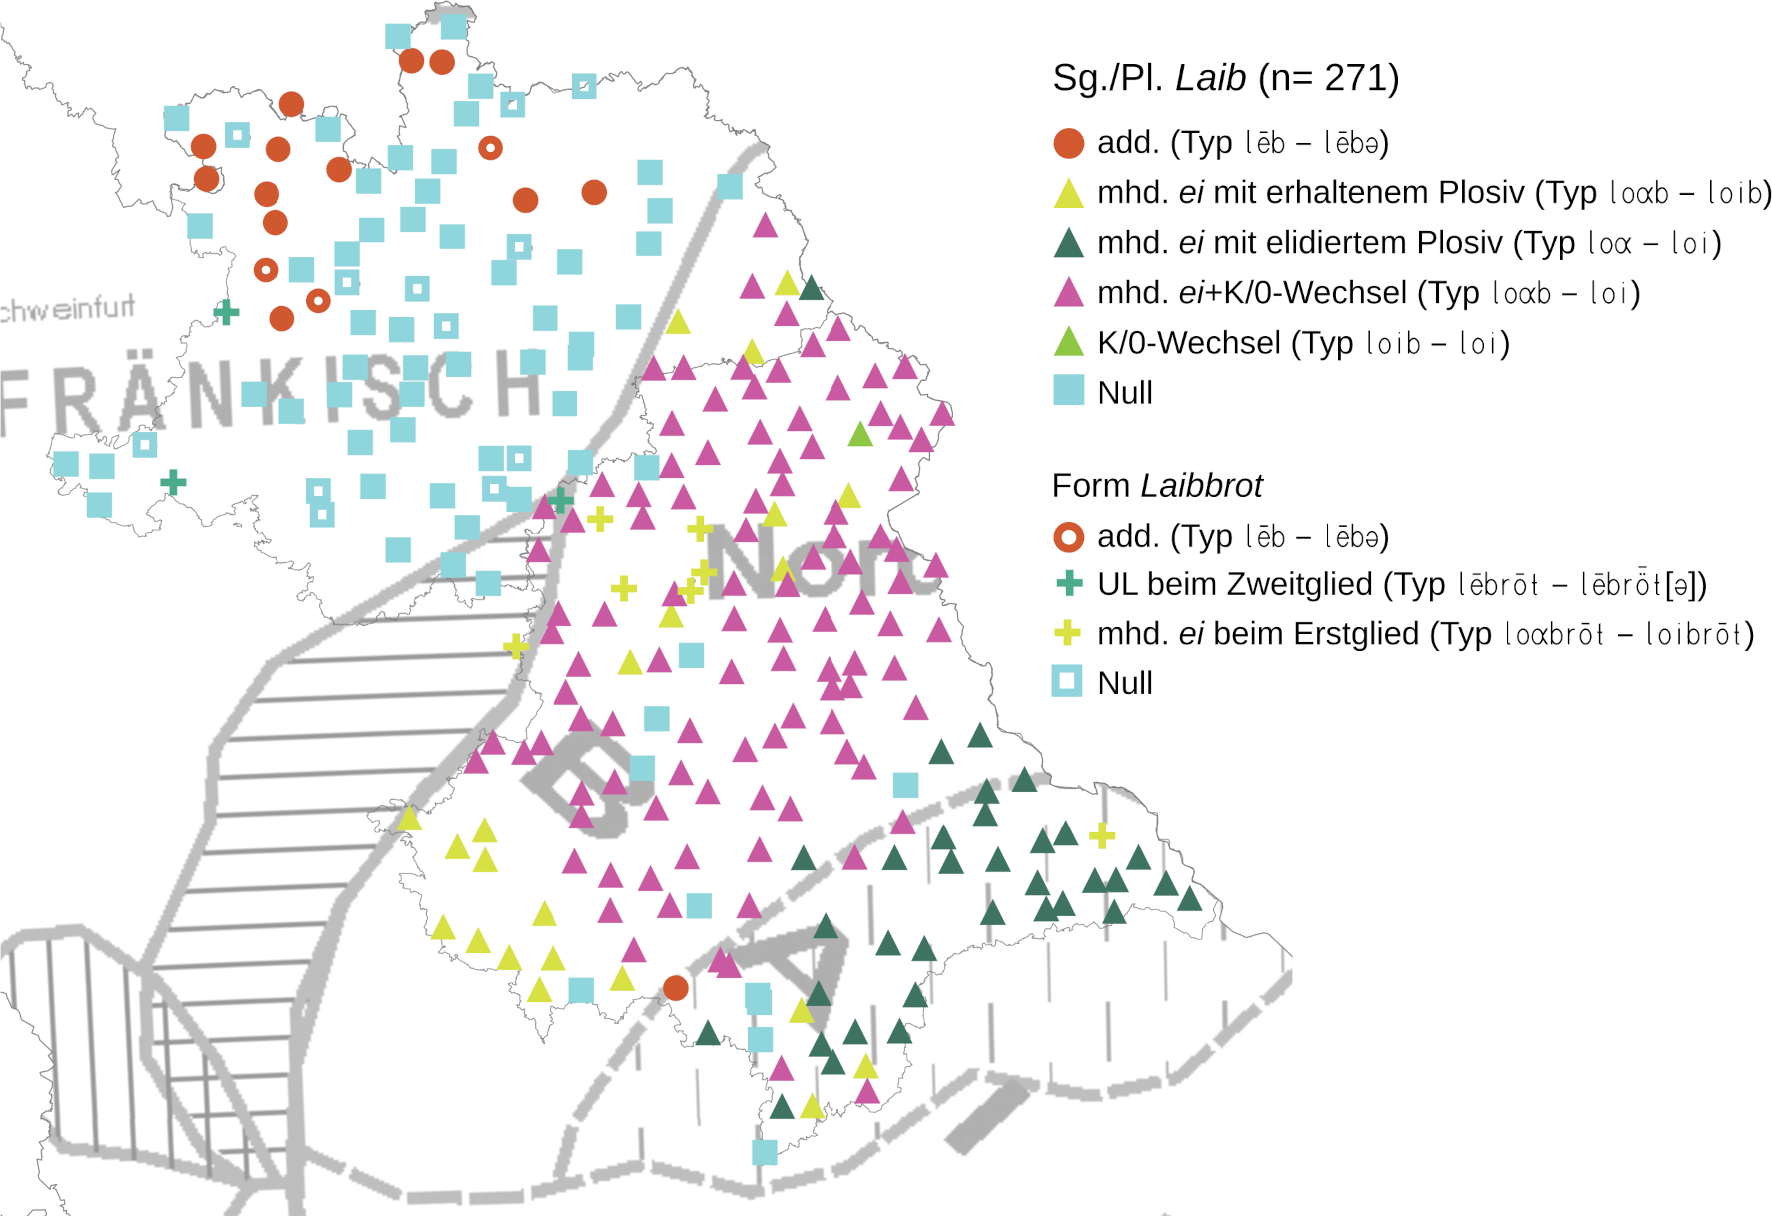
\includegraphics[width=\textwidth]{figures/Karte16.png}
\caption{Pluralmarkierung bei \textit{Laib} im SNOB}
\label{map:16}
\end{map}

Neben den 0/K-Alternationen in stammaffizierenden und additiven Pluralformen wurde in \mapref{map:15} auch die absolute Vorkommenshäufigkeit von K/0-""Al\-ter\-na\-tio\-nen dargestellt. Es zeigt sich, dass Alternationen des Typs \teuthoo{loAb}{loαb} -- \teuthoo{loi}{loi} ‚Laib‘ nur im mittleren und nördlichen Nordbair. vorkommen. In der Literatur werden für die K/0-Alternation im Nordbair. nur vereinzelte Belege angeführt (z.\,B. zum nordbair. Eslarn \citealt[86]{Bachmann2000}, für das Egerländische \citealt[122]{Roth1940}). Um die tatsächliche areale Verbreitung und areale Geltung dieser Form der Konsonantismusalternation zu ermitteln, habe ich sämtliche Rohdaten der entsprechenden Fragen zu Sg./Pl. \textit{Laib} für das nordostbayerische SNOB-Gebiet ausgewertet (\mapref{map:16}).\footnote{\textrm{Für 181 Untersuchungsorte des SNOB-Teilprojekts konnten keine Singular- und Pluralformen ausgewertet werden, da die Transkripte (noch) nicht in der} \textrm{\textit{BayDat}} \textrm{hinterlegt sind oder die Formen nicht abgefragt wurden. Zudem konnte ein Teil der Antworten der Gewährspersonen nicht berücksichtigt werden, da die Gewährspersonen ein Heteronym verwendet haben oder die Segmentierung der Transkripte nicht eindeutig war: Im Fragebuch wurde neben dem Simplex} \textrm{\textit{Laib}} \textrm{auch} \textrm{\textit{Laib Brot}} \textrm{und das Kompositum} \textrm{\textit{Laibbrot}} \textrm{suggeriert, das im SNOB-UG teilweise üblich ist. Wurde die Form} \textrm{\textit{Laibbrot}}\textrm{/}\textrm{\textit{Laib Brot}} \textrm{in nur einer der Formen realisiert, konnte der Beleg in der Regel nicht ausgewertet werden, da die Klassifikation der Realisierung des auslautenden Plosivs einzig anhand der} \textrm{\textit{BayDat}}\textrm{{}-Kodate nicht unsicher ist.}} Die Variantenverteilung in \mapref{map:16} illustriert, dass die K/0-Alternation für die Singular- und Pluralform von \textit{Laib} des Typs \teuthoo{loAb}{loαb} -- \teuthoo{loi}{loi} ein spezifisch nordbair. Phänomen. ist. Im gesamten nordbair. Teil des UG findet sich der umlautähnliche Diphthongwechsel von mhd. \textit{ei} (vgl. \sectref{sec:7.1.2.1.2}). Im nordbair.-mittelbair. Übergangsgebiet ist /b/ im primären und sekundären Auslaut entfallen (Typ \teuthoo{loA}{loα} -- \teuthoo{loi}{loi}), im Südwesten der Oberpfalz und vereinzelt im nördlichen Nordbair. ist /b/ im primären und sekundären Auslaut erhalten (Typ \teuthoo{loAb}{loαb} -- \teuthoo{loib}{loib}). Im Norden des ofr. Teils des UG wird der Plural von \textit{Laib} additiv gebildet, im übrigen Gebiet des Ofr. findet sich Nullplural (vereinzelt auch im Nordbair.).

Zwei weitere Belege für K/0-Wechsel im Nordbair. finden sich in den vorliegenden Daten für die Vokal-Konsonantenfolge /Vd/: \teuthoo{mo2Ad}{mōαd} -- \teuthoo{mo9.2i}{mo\klammeruntenpost{}̄ͅi} ‚Magd‘ und die suggerierte Form \teuthoo{ro2d}{rōd} -- \teuthoo{re42}{rẹ̄} ‚Rad‘ (neben \teuthoo{ra42dl@}{rạ̄dl̥} -- \teuthoo{ra42dl@n}{rạ̄dl̥n}) im nordbair. Nabburg. Die Pluralform für \textit{Magd} wird wie auch bei \textit{Laib} im nordbair. UG durch stammaffizierende Markierung gebildet, weshalb eine weitere Kartierung des gesamten SNOB-Materials als Vergleichskarte sinnvoll erschien.\footnote{Für das Neutrum \textit{Rad} finden sich vor allem Pluralformen des Typs \textit{Rad} -- \textit{Räder}. Eine erste Durchsicht der SNOB-Rohdaten in \textit{BayDat} hat allerdings eine weitere Form für ofr. Blankenberg (Thüringen) ergeben: \teuthoo{ro.ûud}{rỗ̃ͅ{\aufstrih}ud} -- \teuthoo{re:2}{re{\doubleogonek}̄} ‚Rad‘.} \mapref{map:17} zeigt, dass sich die Variante \teuthoo{moAd}{moαd} -- \teuthoo{moi}{moi} mit K/0-Alternation in einem ähnlichen, aber kleineren Areal findet wie bei \textit{Laib}. Im Nordosten des Nordbair. ist die Varianten mit erhaltenem Plosiv im primären und sekundären Auslaut belegt (Typ \teuthoo{moAd}{moαd} -- \teuthoo{moid}{moid}).\footnote{Vgl. \citet[124]{Roth1940} zur Konsonanten-Alternation K/0 im Egerländischen: „Die Form \textit{mei} ist nur im Ascher Land und in der nordöstlichen Übergangszone erhalten, sonst herrscht \textit{mēid}.“}

\begin{map}
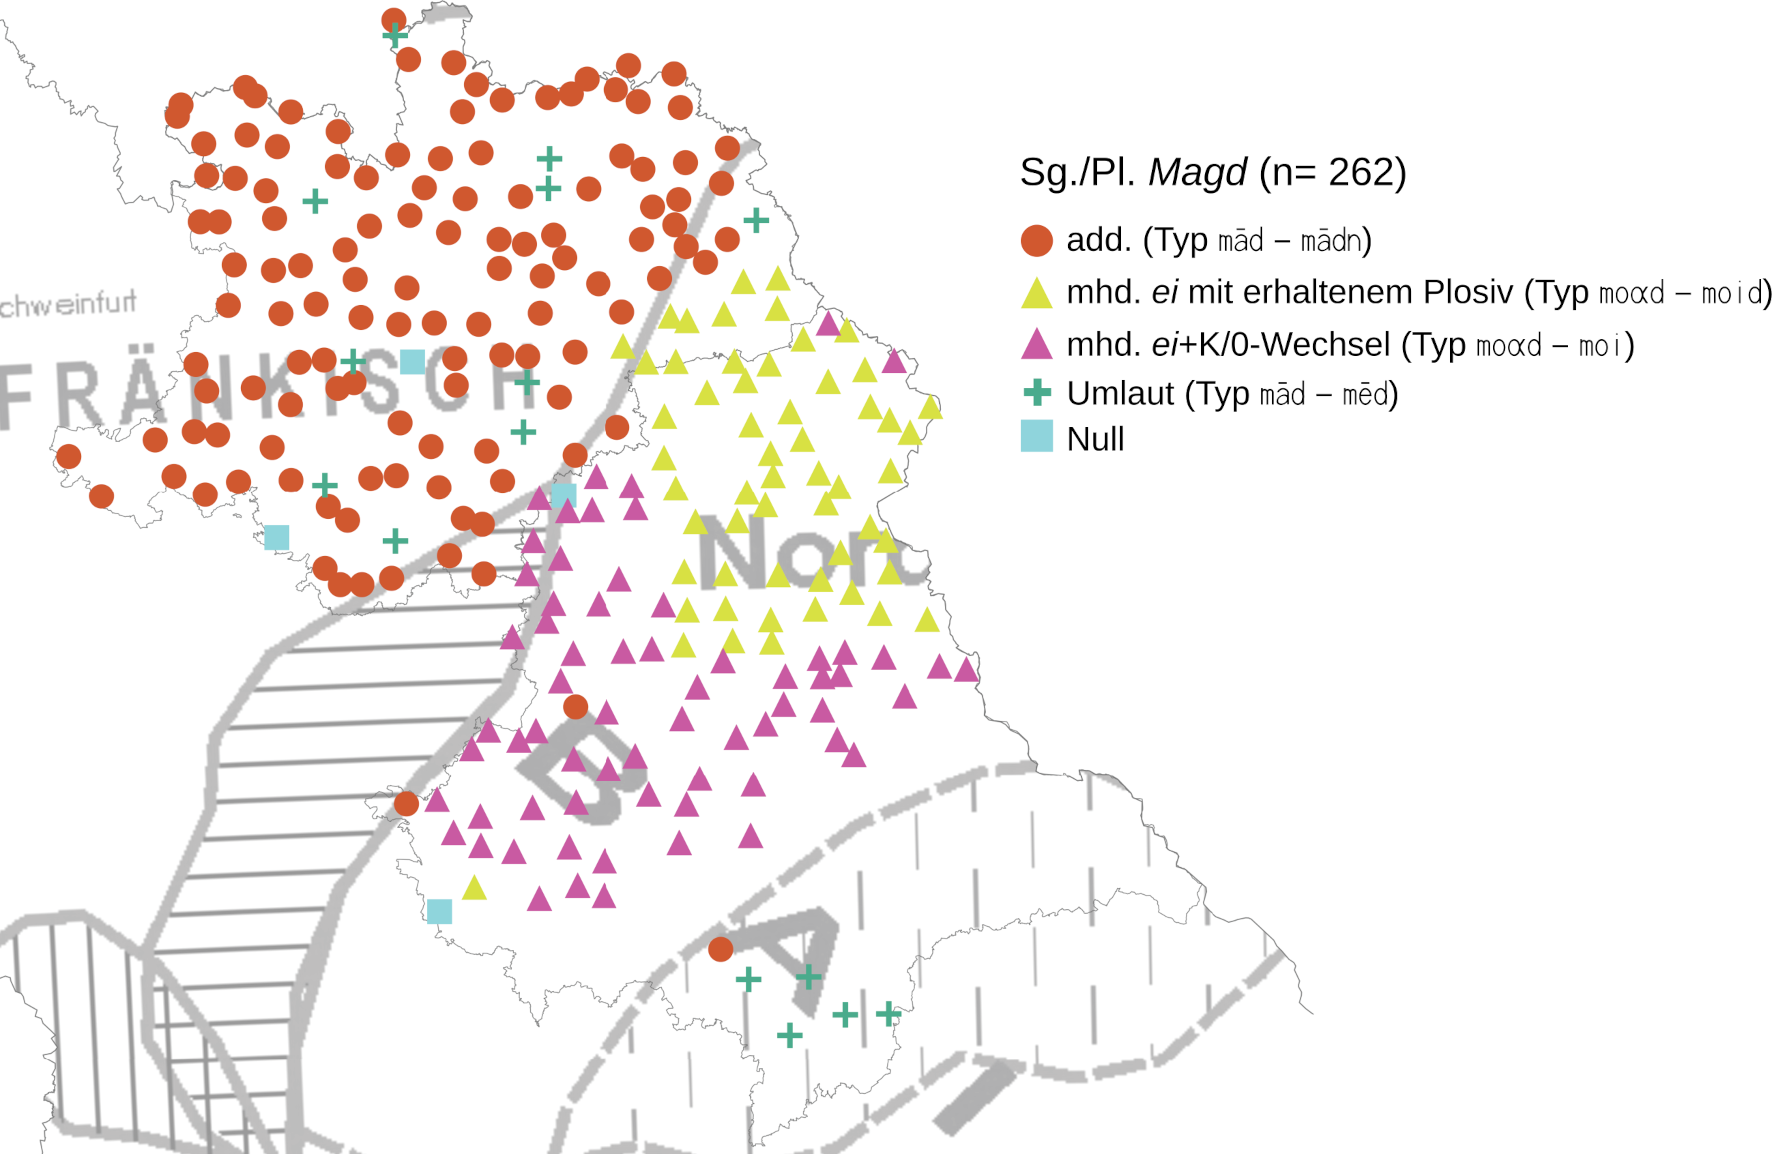
\includegraphics[width=\textwidth]{figures/Karte17.png}
\caption{Pluralmarkierung bei \textit{Magd} im SNOB\protect\footnote{Das Heteronym \textit{Dirn} im Süden des UGs wurde nicht kartiert.}}
\label{map:17}
\end{map}

Wie auch bei subtraktiver Morphologie im phonologischen Kontext von Vokal-Konsonant-Abfolgen sind die dargestellten innerparadigmatischen Konsonantismusalternationen das Ergebnis von Lenisierungen (vgl. \citealt[82]{Birkenes2014}). Anders als bei \citeauthor{Birkenes2014}' (\citeyear{Birkenes2014}) subtraktiven Flexionsformen ist Lenisierung im Bair. nicht nur in intervokalischer Umgebung, sondern auch im absoluten Auslaut wirksam; in unterschiedlichen phonologischen Umgebungen tritt sie im primären und im sekundären Auslaut ein. Bei Singular-/Pluralformen des 0/K-Typs ist der Konsonant im absoluten Auslaut der Singularform elidiert, in der (ehemals) intervokalischen Position der Pluralform aber erhalten (bzw. beim 0/0-Typ auch in dieser Position elidiert). In Teilen des Nordbair. ist -- lexemweise -- der auslautende Plosiv im primären Auslaut der Singularform erhalten, aber im sekundären Auslaut der Pluralform getilgt, weshalb die Formen mit K/0"=Konsonantenalternation in diesem Gebiet zu finden sind. Inwiefern diese Formen der Pluralmarkierung produktiv sind oder ob es sich um Relikte der phonologischen Prozesse der mittelbair. Konsonantenschwächung handelt, kann mit den vorliegenden Daten nicht beantwortet werden; zumindest konnten sie nicht außerhalb der bekannten phonologischen Kontexte nachgewiesen werden. Es scheint sich also um lexikalisierte morphophonologische Alternationen zu handeln. Während die 0/K"=Alternationen im Nord- und Mittelbair. als „längere“ Pluralformen mit erhaltenem Konsonanten dem Prinzip „Mehr Inhalt, mehr Form“ entsprechen, laufen K/0"=Alternationen -- wie subtraktive Pluralformen auch -- diesem Prinzip entgegen: Semantisches Mehr wird hier durch weniger Form kodiert.

\subsubsubsubsection{Elision des finalen Plosivs in Konsonantenclustern}\largerpage[-1]

Beide Muster der innerparadigmatischen Konsonantismusalternation (0/K, K/0) finden sich auch für die finalen Plosive in Konsonantenclustern, sie sind hier das Ergebnis von Konsonantenassimilation. Zwar können an dieser Stelle nur Tendenzen aufgezeigt und exemplarische Fälle diskutiert werden, da -- wie \mapref{map:18} illustriert -- in den BSA-Erhebungen für die einzelnen Konsonantencluster nur wenige Items abgefragt wurden. Gleichzeitig geben diese exemplarischen Fälle Einblicke in die spezifisch dialektale Formenbildung und eröffnen grundsätzlichere Fragen der Flexionsmorphologie, wie weiter unten gezeigt wird.

Für die einzelnen Lexeme mit finalem Konsonantencluster haben Konsonantismusalternationen im UG zum Teil großräumige, teilweise aber auch recht kleinräumige regionale Geltung. Innerparadigmatische Alternationen bei additiven Pluralformen finden sich für das Konsonantencluster /ld/ im Neutrum \textit{Feld} (K/0"=Alternation \teuthoo{vôe"?l.d.}{v{\aufstrih}ë̄lͅdͅ} -- \teuthoo{vôe.l.A}{v{\aufstrih}eͅlͅα} neben 0/K"=Alternation \teuthoo{ve.2i“.}{vēͅīͅ} -- \teuthoo{ve.2i“dA).}{vēͅīdα\klammeruntenpost{}ͅ}\footnote{Im Ofr. erfolgt für die /ld/-Abfolge teilweise die Assimilation des Dentalplosivs in intervokalischer Position, \citet[§28c]{Kranzmayer1956} nennt die assimilierten Formen daneben für das Nord- und Mittelbair. (mit Ausnahme weiter Teile Ober- und Niederbayerns, vgl. \citealt[400]{Schirmunski1962}, vgl. \citealt{WA}-Karte 524 „Felde“). Auch \citet[69f.]{Birkenes2014} führt die Assimilation für Teile des Ofr. und das Nordbair. an und kann für diesen Teil des UGs in den untersuchten Dialektgrammatiken für \textit{Feld} und \textit{Wald} auch subtraktive Dativformen nachweisen.} In Na\-sal+Plo\-siv-""Kon\-so\-nan\-ten\-clus\-tern ist die homorgane Sequenz aus Nasal und Plosiv (/mb/, /nd/) in intervokalischer Position in einem Teil des UGs assimiliert (vgl. \citealt[392--395]{Schirmunski1962}, \citealt[§28c2]{Kranzmayer1956}, \citealt{WA}-Karte 545 „hinten“). Im Ofr. und teilweise im Nordbair. ist der Dentalplosiv im absoluten Auslaut gleichzeitig erhalten, sodass K/0-Alternation bei den additiven Pluralformen von \textit{Kind} erscheinen, z.\,B. \teuthoo{A}{α} \teuthoo{gsu.nds}{ɡsuͅnds} \teuthoo{k\_i.nd}{kʰiͅnd} -- \teuthoo{di.}{diͅ} \teuthoo{k\_i.nA}{kʰiͅnα} (‚Kind‘, ofr. Mitteleschenbach).\footnote{In \citeauthor{Birkenes2014}' (\citeyear[56]{Birkenes2014}) Analyse entspricht das /nd/-Konsonantencluster der phonologischen Umgebung, für die sich die meisten Belege subtraktiver Morphologie nachweisen lassen (vgl. \sectref{sec:7.1.2.4} und die subtraktiven Pluralformen im ofr.-hess. Wiesthal). Schirmunski beschreibt für den ofr. Taubergrund die Assimilation von inlautendem \textit{nd} > \textit{n} auch nach Apokope des Schwa-Suffixes: \textit{hū\textsuperscript{n}}\textit{nt} -- \textit{hü\textsuperscript{n}}\textit{n} ‚Hund‘, \textit{wō\textsuperscript{n}}\textit{nt} --\textit{w}\textrm{\textit{e.}}\textit{\textsuperscript{n}}\textit{n} ‚Wand‘, \textit{kī\textsuperscript{n}}\textit{nt} -- \textit{ki\textsuperscript{n}}\textit{n} ‚Kind‘ (< mhd. \textit{kinde}, \citealt[394]{Schirmunski1962}).}



\begin{map}
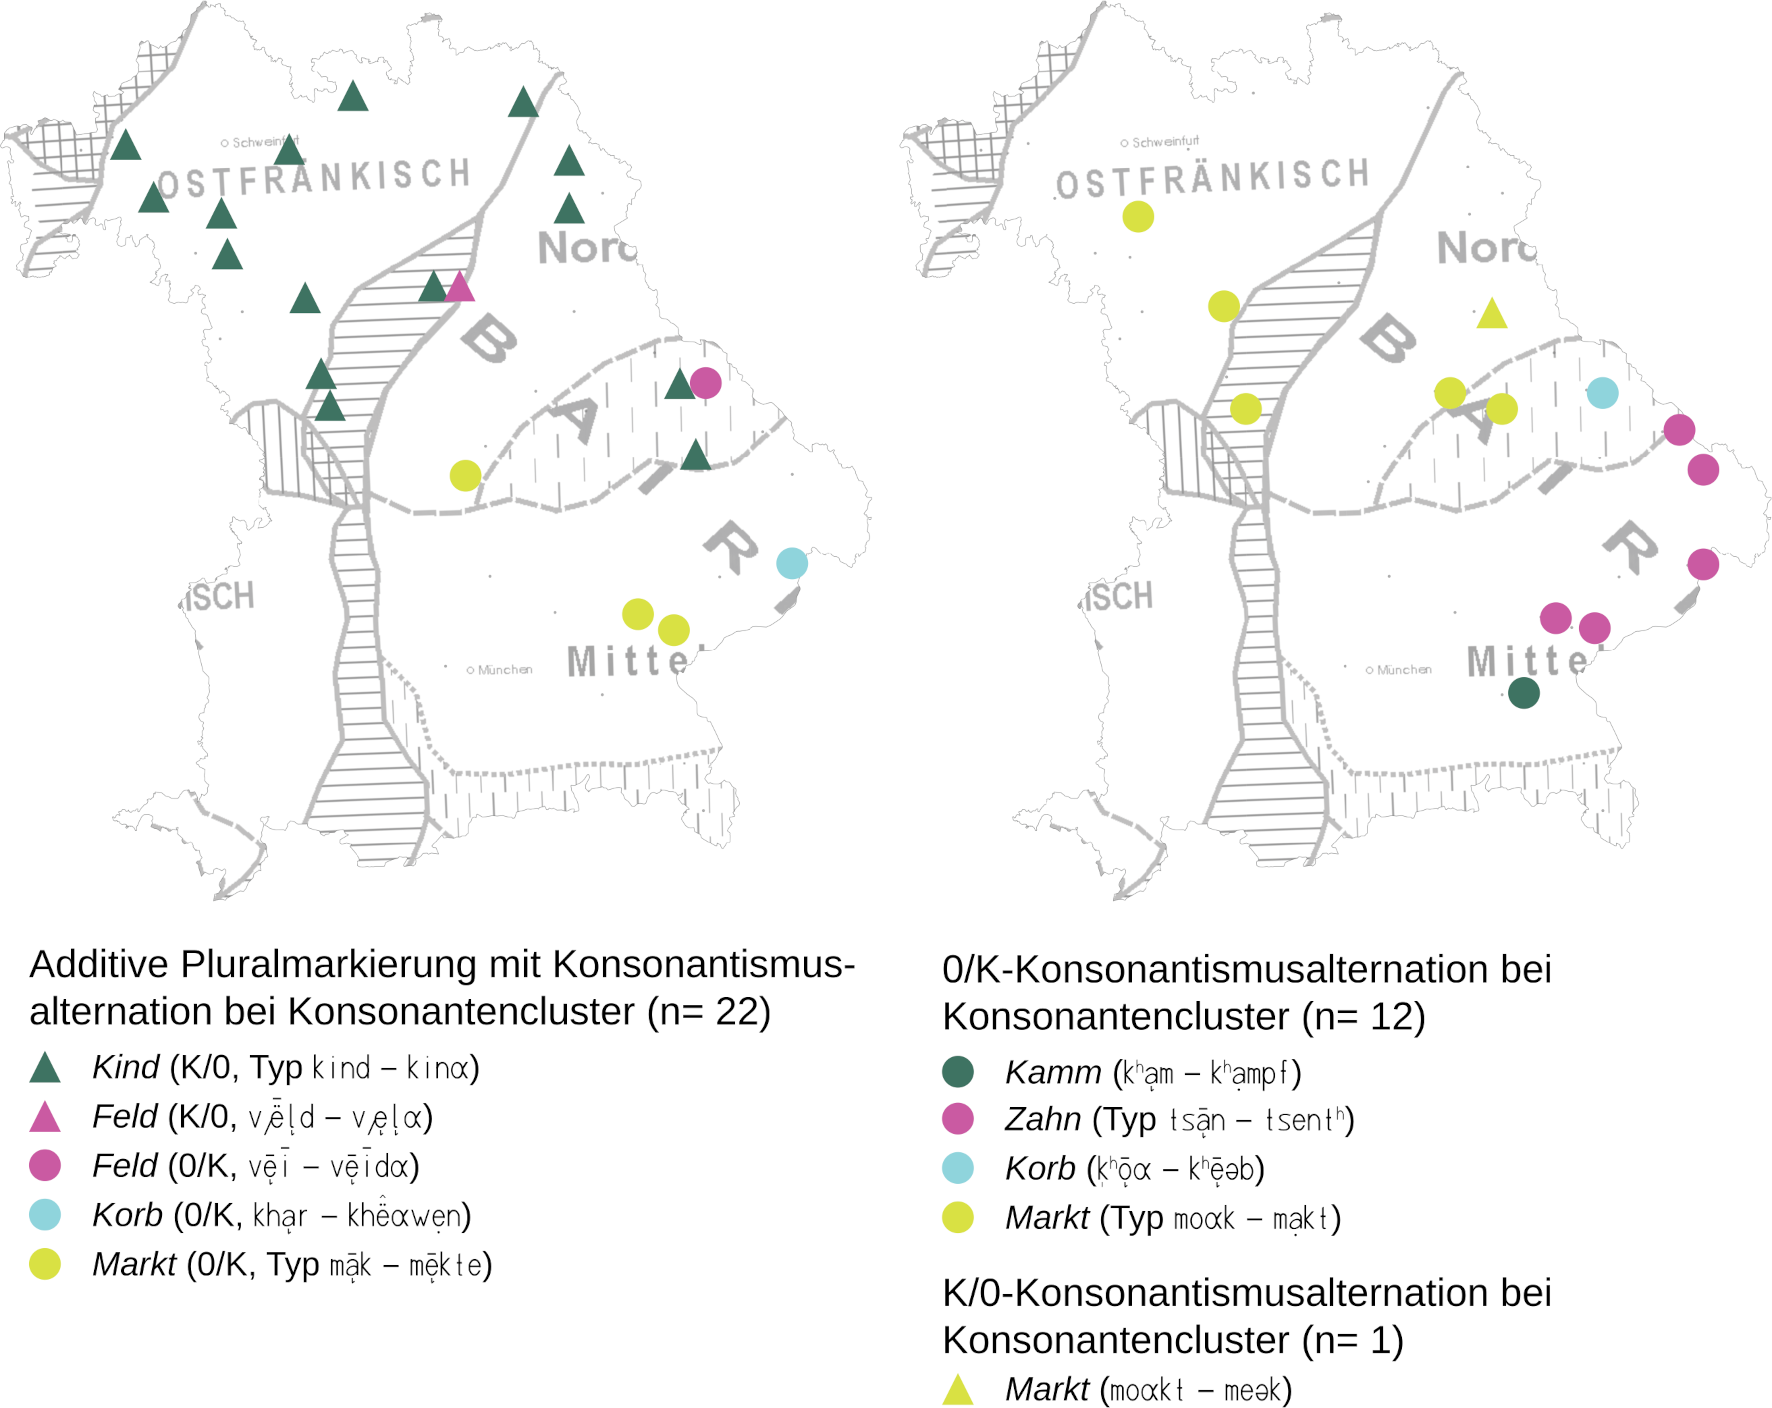
\includegraphics[width=\textwidth]{figures/Karte18.png}
\caption{Belege für Konsonantenelision bei Konsonantenclustern}
\label{map:18}
\end{map}


In stammaffizierenden Pluralformen treten innerparadigmatische Alternationen bei Konsonantenclustern eher im Bair. auf.\footnote{Nur für die Liquid+Plosivfolge in \textit{Markt} finden sich auch im Ofr. Formen mit elidiertem finalen /t/ in der Singularform von \textit{Markt} und erhaltenem /t/ im Plural (vgl. 	\tabref{tab:31}). \citet[127]{Roth1940} erwähnt daneben Fälle von Elision des auslautenden \textit{t} in der Umgebung von Fortisplosiven aus dem Egerländischen: \teuthoo{mo.Ek}{moͅək} ‚Markt‘, \teuthoo{lo.2Es}{lōͅəs} neben \teuthoo{lo.2sd}{lōͅsd} (Pl. \teuthoo{lo.isn4}{loͅisṇ}, ‚(Schuhmacher-)Leiste‘).} Trotz der geringen Belegdichte illustriert die Durchsicht von stammaffizierenden Markierungen bei Nasal-Plosiv-Abfolgen, in welchem Maße sich phonologische Prozesse und Pluralmarkierungsstrategien (respektive lexemspezifische Pluralformen) in den Dialekten bedingen. So ergeben sich im UG für die homorgane Sequenz aus Nasal und Dental in \textit{Kamm} (nhd. \textit{Kamm} < mhd. \textit{kamp} neben \textit{kam}, vgl. \citealt[I.783b]{Lexer1872-1878}) und \textit{Zahn} (ahd. \textit{zand}, mhd. \textit{zant} neben \textit{zan}, vgl. \citealt[III.848a]{Lexer1872-1878}) unterschiedliche Alternationsmuster mit erhaltenem vs. assimiliertem Finalplosiv je nach phontaktischer Position:\largerpage[-1]

\begin{itemize}
\item Für die /mb/-Abfolge in \textit{Kamm} erscheinen in einem Großteil der nieder-, mittel- und oberdeutschen Dialekte wie auch in der Standardsprache infolge der regelmäßig durchgeführten Assimilation des Labialplosivs im Aus- und Inlaut keine innerparadigmatische Alternation (Wechseltypus 0/0, z.\,B. \teuthoo{kha9.m}{kha\klammeruntenpost{}ͅm} -- \teuthoo{khe.m}{kheͅm} ‚Kamm‘, \teuthoo{khe94mA}{khe\klammeruntenpost{}̣mα} ‚kämmen‘ im ofr. Burgbernheim).
\item In Teilen des Ofr. (neben dem West- und Ostmitteldeutschen) ist die Assimilation von /mb/ in \textit{Kamm} nur im ehemaligen Inlaut (der additiven Pluralformen) durchgeführt, sodass synchron subtraktive Formen erscheinen: \teuthoo{kha."+mb\_}{khã̄ͅmbʰ} -- \teuthoo{khe.m}{kheͅm} ‚Kamm‘, \teuthoo{khemE}{khemə} ‚kämmen‘ im ofr.-hess. Wiesthal (vgl. \sectref{sec:7.1.2.4} sowie \citealt[76--78]{Birkenes2014}, \citealt[392--393]{Schirmunski1962}, \citealt[Karte 162]{SUF1}, \citealt[Karte 26]{SUF3}).
\item In konservativeren bair. Dialekten ist das Muster der Alternation ein anderes (mit anderen Worten: typisch bairisches), da das /b/ in der Finalposition im Singular assimiliert, in der Pluralform im sekundären Auslaut erhalten ist, z.\,B. \teuthoo{kha.m}{khaͅm} -- \teuthoo{kha4mb5\_}{khạmb̩ʰ} ‚Kamm‘, \teuthoo{k\_a94mb5e4n}{kʰa\klammeruntenpost{}̣mb̩ẹn} ‚kämmen‘ im nordbair.-mittelbair. Blaibach. Auch für die Nasal-Plosiv-Abfolge in \textit{Zahn} finden sich in Teilen des Bayerischen Waldes und des Rottals innerparadigmatische Alternationen durch Erhalt des ehemals intervokalischen /d/, z.\,B. \teuthoo{tSa2):n}{tʃā\klammeruntenpost{}{\doubleogonek}n} -- \teuthoo{tSe.nt\_}{tʃeͅntʰ} im nordbair.-mittelbair. Zwiesel (vgl. \citealt[§28c]{Kranzmayer1956}, \citealt[Karte 82]{SOB4}, \citealt[32 und 160]{SNiB4}).
\item Bei Erhalt des Plosivs auch im primären Auslaut erscheinen in den mittelbair. Tiefenbohrungspunkten lautgesetzlich entstandene Le\-nis-""For\-tis-""Kon\-tras\-te, z.\,B. \teuthoo{ka.<mb\%v\%}{kâͅmb͈v͈} -- \teuthoo{kha4mpf}{khạmpf} ‚Kamm‘ im mittelbair. Niedertaufkirchen, \mbox{\teuthoo{d5s5a.26d.}{d̩s̩ã̄ͅdͅ}} -- \teuthoo{tSe9.nt\_}{tʃe\klammeruntenpost{}ͅntʰ} im mittelbair. Waldhof.\footnote{Dass in den bair. Dialekten lexemweise eine hohe Varianz der formalen Realisierung \textrm{innerparadigmatischer Konsonantismusalternationen} im \textrm{interdialektalen Vergleich besteht,} zeigen auch \textrm{die Singular- und Pluralformen von} \textit{Korb}\textrm{. Ist der finale Plosiv der Liquid-Plosiv-Abfolge im Singular elidiert, in der (ehemals) intervokalischen Position des Plural aber erhalten, erscheinen innerparadigmatische Alternationen: \teuthoo{k,\_o.<A}{k͓ʰôͅα} -- \teuthoo{k\_e.<Eb5}{kʰêͅəb̩} im n}ordbair.-mittelbair. Grafenkirchen, \teuthoo{kha.r}{khaͅr} -- \teuthoo{khe>?Awe4n}{khë̂αwẹn} \textrm{im} mittelbair. Neukirchen am Inn. Ist der finale Plosiv in beiden Positionen erhalten, können innerparadigmatische Lenis-Fortis-Kontraste als Pluralmarkierungsstrategie funktionalisiert sein: \teuthoo{kho<Erb}{khôərb} -- \teuthoo{kherp}{kherp} im nordbair. Tirschenreuth.}
\end{itemize}

\subsubsubsubsection{Flexionsmorphologische Klassifikation der Obstruenten-Elision}
\begin{sloppypar}
Die konkrete formale Realisierung von stammaffizierenden Verfahren ist bei Stämmen mit auslautendem Obstruenten in hohem Maße durch das Eintreten (bzw. Nicht-Eintreten) von phonologischen Prozessen (Elision und Assimilation) bedingt. Da es hier für die einzelnen Lexeme im UG zum Teil großräumige, teilweise aber auch recht kleinräumige regionale Schwankungen gibt, ergibt sich ein ausgesprochen buntes Bild innerparadigmatischer Alternationen und der konkret belegten Pluralformen. Ist die Annahme eines Pluralmarkers „Konsonantismuskontrast“ hier sinnvoll, konstituiert er spezifische Deklinationsklassen? Für jene Fälle, die sich synchron „kaum auf einen gemeinsamen Nenner“ bringen lassen und regional stark schwanken, schlägt \citet[124]{Rowley1997} eine Klassifikation als (schwache) Suppletion vor.\footnote{\citet[217--218]{Schnabel2000} subsumiert in seiner synchronen Substantivklassifikation (die auch die Diminutivbildung einschließt) sogar Fälle als „schwache Suppletion“, die mit Blick auf die historisch-phonologische Entwicklung der Singular- und Pluralformen in dieser Arbeit als Konsonantismusalternationen (d.\,h. als stammaffizierende Markierung) gewertet werden würden, z.\,B. \teuthoo{gxI+"d}{ɡxı̃̄d} -- \teuthoo{gxine}{ɡxine} ‚Kind‘, \teuthoo{gxo+"b}{ɡxȭb} -- \teuthoo{gxem}{ɡxem} ‚Kamm‘, \teuthoo{bu2}{bū} -- \teuthoo{bum}{bum} ‚Bube‘.} Nur für das nordbair.-mittelbair. Übergangsgebiet im Bayerischen Wald führt \citet[124]{Rowley1997} so viele Fälle von innerparadigmatischer Konsonantenelision an, dass es „ökonomischer“ scheine, ein eigenes Flexionsmuster des Wechseltyps 0/K anzusetzen.
\end{sloppypar}

Alternativ zu dieser Klassifikation schlage ich eine Differenzierung innerparadigmatischer Konsonantismuselisionen bei additiven vs. stammaffizierenden Pluralmarkierungen vor, die die Formenbildung der Plural- und weniger die der Singularform fokussiert. 0/K-Alternationen in additiven Formen (Typ \teuthoo{vi“}{vī} -- \teuthoo{vi“cA}{vīXα}) sind -- ähnlich wie innerparadigmatische Spirantisierungen (\sectref{sec:7.1.2.3.3}) -- in stärkerem Maße phonologisch konditioniert, während 0/K- und K/0-""Al\-ter\-na\-tio\-nen als stammaffizierende Verfahren in den bair. Dialekten in kombinierten Markierungen (Typ \teuthoo{bao}{bao} -- \teuthoo{baeX}{baeꭗ}) oder als alleinige formale Marker der Pluralinformation (z.\,B. \teuthoo{we42}{wẹ̄} -- \teuthoo{we42g}{wẹ̄ɡ} ‚Weg‘ im nordbair.-mittelbair. Zwiesel) eher auf der morphologischen Ebene funktionalisiert sind. Damit ergibt sich für die bair. Dialekte ein spezifisches Flexionsmuster mit elidiertem Obstruenten im Singular und erhaltenem Obstruenten im Plural, die konkrete Realisierung ist dann möglicherweise lexemspezifisch im Lexikon abgespeichert.

\citet[19]{White1966} stellt bei jüngeren Sprechern des westmittelbair. Dialekts von Eisenhofen einen Abbau der innerparadigmatischen Alternationen zwischen elidiertem und erhaltenem Konsonanten fest („teils durch Systemzwang, teils infolge hochsprachlichen Einflußes“).\footnote{Bereits \citet[§111.2b]{Gebhardt1907} stellt den Abbau von Elisionen durch innerparadigmatischen Ausgleich für das Nürnberger Ofr. fest, z.\,B. in \textit{waib} ‚Weib‘, \textit{grob} ‚Grab’und \textit{loib} ‚Laib‘.} In additiven Pluralformen des Typs \teuthoo{we}{we} > \teuthoo{weg}{weɡ} -- \teuthoo{wega}{weɡa} ‚Weg‘ \citep[45]{White1966} entfällt durch den Dialektwandel zwar die innerparadigmatische Alternation, die Pluralform ist aber weiterhin distinkt. Es braucht weitere diachrone Daten, um zu zeigen, ob der Abbau des Dialektmerkmals auch in rein stammaffizierenden Formen des Typs \teuthoo{we42}{wẹ̄} -- \teuthoo{we42g}{wẹ̄ɡ} ‚Weg‘ stattfindet. Hier stellt die 0/-K-Alternation das einzige Pluralmerkmal dar, ein Abbau der Alternation würde den Wechsel in die Nullflexion bedeuten.

\subsubsubsubsection{Nasalelision}

Im gesamten UG (mit Ausnahme einiger Gebiete im Norden Bayerns, vgl. \citealt[59]{RennKönig2006}) ist die Elision von Nasal im Auslaut eingetreten (vgl. \citealt[§46]{Kranzmayer1956}, \citealt[125]{Rowley1997}, \citealt[112]{Roth1940}, \citealt[385]{Schirmunski1962}). Außer im Ofr. in Unterfranken und im Westen wird der Vokal „als Reflex des ursprünglichen Nasalkonsonanten“ (\citealt[59]{RennKönig2006}) nasaliert realisiert, z.\,B. \teuthoo{mo:"+}{mō{\doubleogonek}̃} ‚Mann‘ (nordbair. Nabburg), \teuthoo{s\#d\%o>+A+:"+}{šd͈ỗα̃̄{\doubleogonek}̃} ‚Stein‘ (mittelbair. Neukirchen am Inn).\footnote{Vgl. \citet[74]{Rowley1997}, \citet[128]{Schmeller1821} sowie \citet[11]{Schießl1909} zum Mittelbair. und zum Ofr. \citet[§95.1]{Gebhardt1907}.}  Erhalt vs. Elision des auslautenden Nasals wurde getrennt für die mhd. Kurz- und Langvokale und Diphthonge untersucht, da die Nasaltilgung sowohl in der Stellung nach kurzem wie langem Vokal für einzelne Wörter und „je nach der grammatischen Form und Funktion“ \citep[385]{Schirmunski1962} unterschiedlich erfolgt ist.

Für die mhd. Kurzvokale (im Korpus belegt sind nur Substantive mit Stammvokal mhd. \textit{a}) zeigt sich, dass die Art des Pluralmarkierungsverfahrens (additiv vs. rein stammaffizierend) den Erhalt bzw. die Tilgung des Nasals bedingt (vgl. \citealt[125]{Rowley1997}). Für \textit{Zahn} (mhd. \textit{zant}, \textit{zan}), das den Plural im UG durch Umlaut markiert, sind nur Formen ohne innerparadigmatische konsonantische Alternation als Wechseltypus 0/0 (Typ \teuthoo{dso2}{dsō} -- \teuthoo{dse2}{dsē} im Ofr. und Nordbair.) oder K/K (Typ \teuthoo{dsa2n}{dsān} -- \teuthoo{dse2n}{dsēn} im Mittelbair.) realisiert. (Ausgenommen werden hier die mittelbair. Formen mit Dentalplosiv im Auslaut, die innerparadigmatische Alternation durch Plosivelision aufweisen, vgl. \mapref{map:18}). Für das additiv-modulative Pluralverfahren des Belegworts \textit{Mann} wird in allen Ortspunkten die Singularform mit elidiertem Nasal, die Pluralform mit Nasal und Pluralsuffix realisiert, z.\,B. \teuthoo{ma."+}{mã̄ͅ} -- \teuthoo{ma."+nA}{mã̄ͅnα} (mittelbair. Waldhof, vgl. \citealt{WA}-Karte 46 „Mann“). Der Stammvokal der Singularform ist gedehnt, was nach \citet[385]{Schirmunski1962} mit der Nasalelision in der Stellung nach kurzem Vokal einhergeht, im Plural erscheint in den bair. Ortspunkten analogischer Langvokal. In den ofr. Ortspunkten wird im Plural Kurzvokal realisiert (z.\,B. \teuthoo{mo42+}{mọ̄̃} -- \teuthoo{me4nE}{mẹnə} in Wilhermsdorf), sodass es neben Kontrasten der Vokalqualität (Umlaut) auch Kontraste der Vokalquantität zwischen Singular und Plural gibt.


\begin{map}
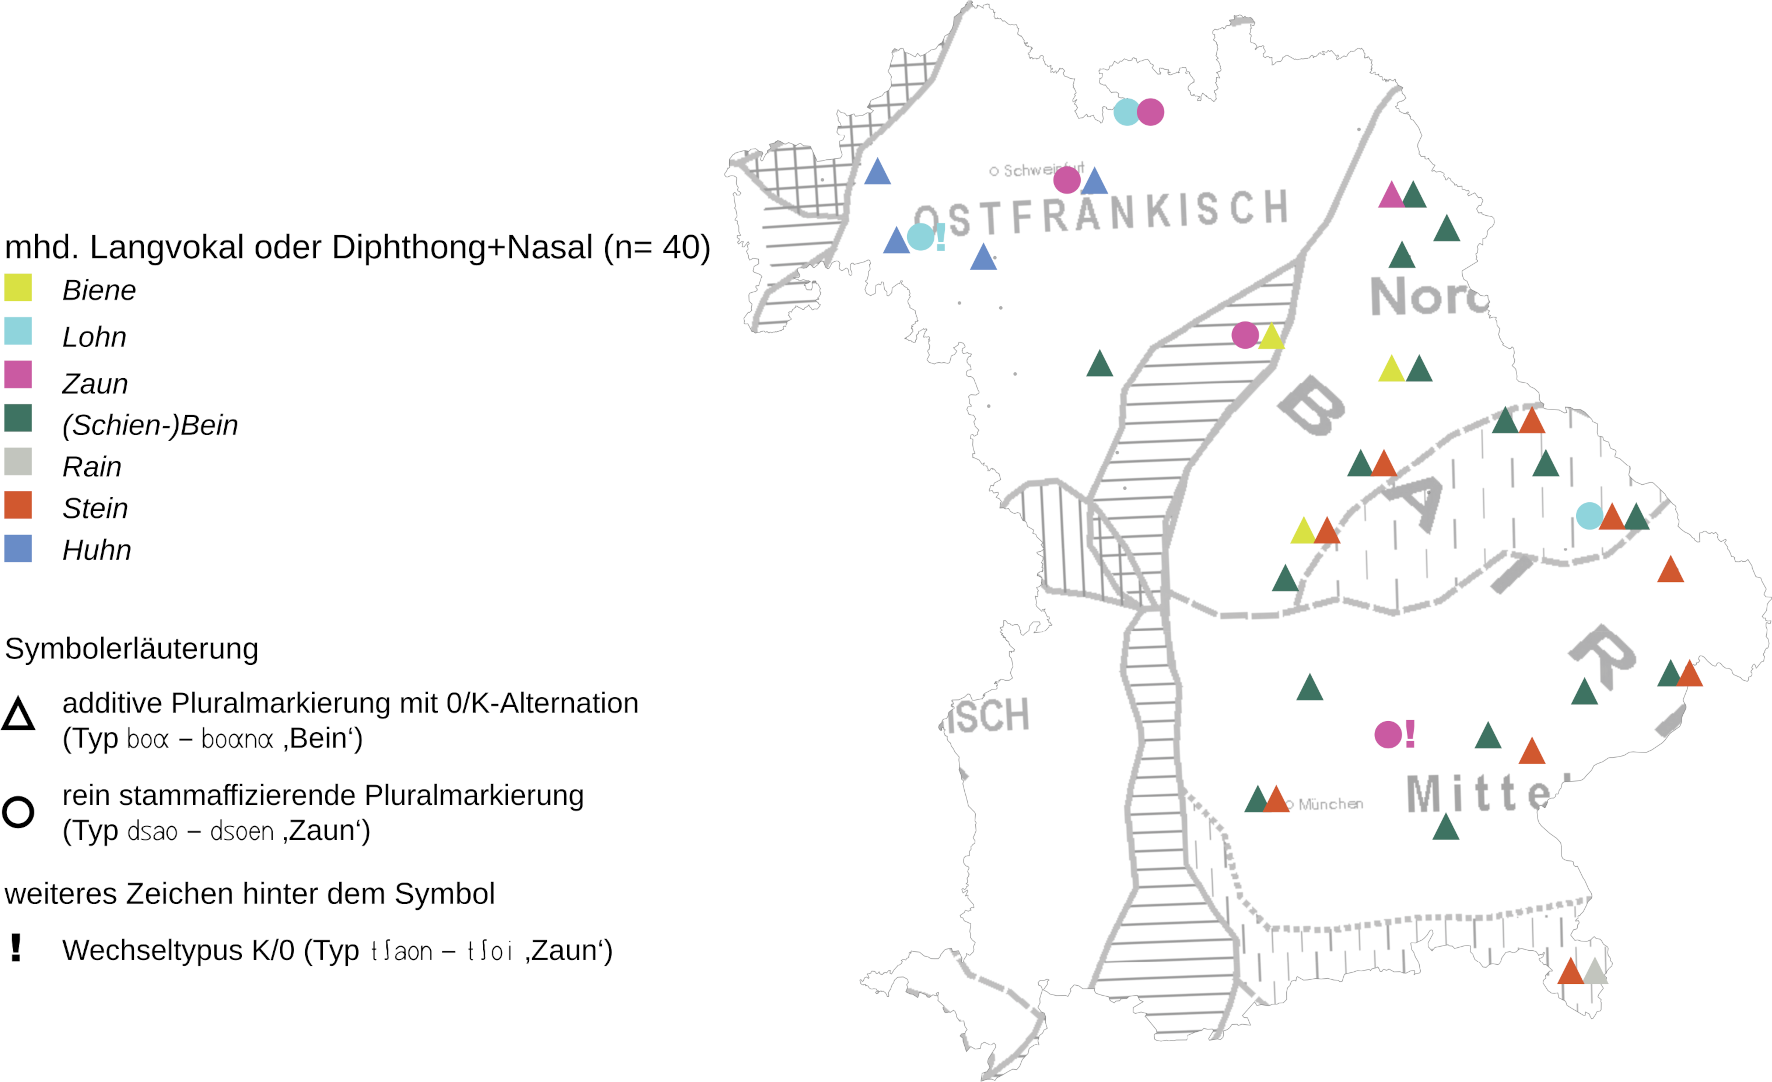
\includegraphics[width=\textwidth]{figures/Karte19.png}
\caption{Innerparadigmatischer Wechsel bei Nasalelision nach mhd. Langvokal und Diphthong im primären und sekundären Auslaut}
\label{map:19}
\end{map}

Auch bei den Substantiven mit mhd. Langvokal oder Diphthong im Stammvokal bedingt v.\,a. das Pluralverfahren, ob der Nasal in der Pluralform realisiert wird (vgl. \citealt{WA}-Karte 224 „Wein“): 83\,\% der Belege mit Nasalelision im Singular markieren den Plural additiv (neben möglicher Vokalmodulation), nur sieben der 40 Fälle (17\,\%) bilden die Pluralform durch ein rein stammaffizierendes Verfahren. \mapref{map:19} zeigt, dass innerparadigmatische Nasalelision lexemweise größere Areale umfasst und ortsdialektspezifisch sein kann.\footnote{Der Nasal nach mhd. \textit{ei} wird in den bair. Tiefenbohrungspunkten im Lexem \textit{Bein} (bzw. \textit{Schienbein}) im Singular überwiegend elidiert, im Mittelbair. und nordbair.-mittelbair. Übergangsgebiet außerdem bei \textit{Stein} sowie als Einzelbeleg \textit{Rain}. In anderen phonologischen Umgebungen (respektive Lexemen) tritt Nasal\-elision nur in einem kleinen Gebiet auf: \textit{Huhn} im Unterofr., \textit{Biene} vereinzelt im Nordbair. Es finden sich außerdem vereinzelte Belege für Nasaltilgung bei \textit{Lohn} und \textit{Zaun} (mit K/0-Alternation im mittelbair. Inning am Holz).} Daneben wird bei Einsilbern in der phonologischen Umgebung vor auslautendem Obstruenten (meist bei eingetretener Einsilberdehnung) der Nasal in einem Teil des UG in der Singularform elidiert: in einem relativ großen Areal im Ofr. und Mittelbair. bei \textit{Gans} sowie vereinzelt im Mittelbair. bei \textit{Gang}, \textit{Kind, Sense} und \textit{Zahn} (mit erhaltenem Plosiv im primären und sekundären Auslaut), z.\,B. \teuthoo{go:2s}{ɡo{\doubleogonek}̄s} (neben \teuthoo{ga):"(+nds}{ɡã̄{\doubleogonek}\klammerobenpost{}\klammeruntenpost{}nds}) -- \teuthoo{gends59}{ɡends̩\klammeruntenpost{}} ‚Gans‘ (ofr. Krum),\footnote{Das auslautende /s/ wird hier als Affrikate realisiert. \citet[§34h1]{Kranzmayer1956} beschreibt das epenthetische [d] zwischen Nasal oder Liquid und Frikativ für das Bair., insb. nach Kurzvokal sei die Epenthese „gemeinbair.“, vgl. Sg. \teuthoo{go.2ns}{ɡōͅns} vs. Pl. \teuthoo{ge.ntß}{ɡeͅntß} im Nord- und Mittelbair.} \teuthoo{s5a4>+s\%d\%\_}{s̩ậ̃s͈d͈ʰ} -- \teuthoo{s\%a4ns5n@}{s͈ạns̩n̥} ‚Sense‘ (mittelbair. Neukirchen am Inn).\footnote{Im Mittelbair. ist Nasalelision außerdem belegt bei \textit{Gang}, \textit{Kind,} und \textit{Zahn} (mit erhaltenem Plosiv im primären und sekundären Auslaut), z.\,B. \teuthoo{ga:"+g.}{ɡā{\doubleogonek}̃ɡͅ} -- \teuthoo{ga4N}{ɡạŋ} ‚Gang‘ (nordbair.-mittelbair. Grafenkirchen), \teuthoo{A}{α} \teuthoo{gás\%und5s5}{ɡ͈s͈und̩s̩} \teuthoo{khi4"4d5}{khị̣̄d̩} -- \teuthoo{k,hindA}{k͓hindα} ‚Kind‘ (mittelbair. Neukirchen am Inn), \teuthoo{d5s5a.26d.}{d̩s̩ã̄ͅdͅ} -- \teuthoo{tSe9.nt\_}{tʃe\klammeruntenpost{}ͅntʰ} ‚Zahn‘ (mittelbair. Waldhof). \citet[75, 125]{Rowley1997} führt außerdem Belege für \textit{Band, Hund} und \textit{Kamm} in Nordbayern an (vgl. \citealt{WA}-Karte 179 „Kind“ und 532 „Hund“; \citealt[§46e und Karte 23]{Kranzmayer1956}, \citealt[16/112]{Roth1940}, \citealt[74 und Karte 16]{Rowley1997}).}

\vfill
\begin{table}[H]
\begin{tabular}{lllll}
\lsptoprule
& {Singular} & {Plural} & {Diminutiv} & \\\midrule
Dorn\footnote{In Erlabrunn mit Nullmarkierung im Pl. (\teuthoo{do42rA94}{dọ̄rα\klammeruntenpost{}̣} - \teuthoo{do42rA94}{dọ̄rα\klammeruntenpost{}̣}).} & \teuthoo{do.2ArE.}{dōͅαrəͅ} & \teuthoo{do.<AnA94}{dôͅαnα\klammeruntenpost{}̣} &  & Gebsattel\\
& \teuthoo{do.2rE.}{dōͅrəͅ} & \teuthoo{dôo?:rnEr}{d{\aufstrih}ö{\doubleogonek}rnər} &  & Ochsenfurt\\
\tablevspace
Horn & \teuthoo{ho.2ArE.}{hōͅαrəͅ} & \teuthoo{h{\textasciitilde}ôo?.rnEr}{h{\aufstrih}öͅrnər} &  & Erlabrunn\\
& \teuthoo{h{\textasciitilde}ôo.2urE}{h{\aufstrih}ōͅurə} & \teuthoo{h{\textasciitilde}ôo.2urE}{h{\aufstrih}ōͅurə}, \teuthoo{hÔe.rnEr}{h{\doppelaufstrih}eͅrnər} & \teuthoo{hElE.}{hələͅ} & Gebsattel\\
& \teuthoo{ho.2rE}{hōͅrə} & \teuthoo{ho?.EnEr}{höͅənər} &  & Ochsenfurt\\
\tablevspace
Kern\footnote{In Gebsattel und Ochsenfurt mit Nullmarkierung im Pl.} & \teuthoo{k\_e.2rE}{kʰēͅrə} & \teuthoo{k\_e.<AnE}{kʰêͅαnə} &  & Gebsattel\\
\tablevspace
Korn & \teuthoo{khôo.2rE}{kh{\aufstrih}ōͅrə} & \teuthoo{kho?.rnE.y}{khöͅrnəͅ⅄} & \teuthoo{khôo>?:E.lE}{kh{\aufstrih}ö̂{\doubleogonek}əͅlə} & Erlabrunn\\
\lspbottomrule
\end{tabular}
\caption{Innerparadigmatische Alternation durch Nasalelision im westlichen Ofr.}
\label{tab:36}
\end{table}
\vfill\pagebreak

Im westlichen Ofr. findet sich für eine kleine Gruppe von Lexemen (\textit{Dorn}, \textit{Horn}, \textit{Kern}, \textit{Korn}) ein dialektraumspezifisches Muster innerparadigmatischer Alternationen (\tabref{tab:36}). In historischen Einsilbern kann hier (wie auch im Schwäbischen) in der phonologischen Umgebung /r/ vor Nasal im Auslaut ein epenthetisches Schwa erscheinen.\footnote{Vgl. \citealt[120 und Karten 60--61]{SBS3}, \citet[389]{Schirmunski1962}, \citealt[Karte 7]{SMF7}, \citealt{WA}-Karte 553 „Korn“; \citet[Karte 18]{Fischer1895}.} In den durch die Epenthese entstandenen zweisilbigen Formen wird der auslautende Nasal elidiert (bei gleichzeitiger Dehnung des Stammvokals in offener Tonsilbe, vgl. \citealt[120]{SBS3}). Da die Schwa-Epenthese nur historische Einsilber betraf, erscheint synchron eine innerparadigmatische Alternation zwischen Epenthese und Nasalelision im Singular und Nasalerhalt im Plural\footnote{In diese Reihe von Substantiven mit /r/-Nasal-Abfolge im Auslaut gehören ebenso \textit{Birne}, \textit{Stern}, \textit{Turm} (wobei \textit{Birne} kein „Sprossvokalwort“ ist, sondern auf mhd. \textit{bir(e)} zurückgeht, sich aber wie ehemalige Einsilber mit -\textit{rn}{}-Folge und Sprossvokal verhält, \citealt[120 und 154]{SBS3}). Die Pluralformen werden in den genannten Ortsdialekten jeweils mit Nullmarkierung bildet. Die Substantive \textit{Arm,} \textit{Darm} und \textit{Wurm} sind in den drei Ortspunkten jeweils mit konsonantischem Auslaut und ohne Sprossvokal belegt; nur im ebenfalls unterofr. Stadtschwarzach erscheint \textit{Arm} im Singular mit elidiertem Nasal (\teuthoo{a4rE}{ạrə} -- \teuthoo{arEm}{arəm}, aber \teuthoo{e.r}{eͅr} \teuthoo{ho.d}{hoͅd} \teuthoo{si.}{siͅ} \teuthoo{E.}{əͅ} \teuthoo{a.m}{aͅm} \teuthoo{gEbro4xN}{ɡəbrọxŋ}) und \textit{Darm} mit epenthetischem Schwa (\teuthoo{da4rEm}{dạrəm} -- \teuthoo{de.rmEr}{deͅrmər}, aber \teuthoo{a4r}{ạr} \teuthoo{ho.ds}{hoͅds} \teuthoo{i.}{iͅ} \teuthoo{dEr}{dər} \teuthoo{da4rm}{dạrm}).}

Die Zusammenschau aller Formen zeigt, dass innerparadigmatische Alternationen zwischen elidiertem vs. erhaltenem Nasal vor allem in additiven Pluralformen auftreten. Wie auch in den vorangegangenen Kapiteln zur innerparadigmatischen Alternation bei Obstruenten stellt sich die Frage: Wie können die verschiedenen Fälle aus flexionsmorphologischer Perspektive modelliert werden? Die Darstellung der lauthistorischen Entwicklung verdeutlicht, dass es sich einerseits um kleinräumige, dialektraumspezifische Entwicklungen handelt und dass die Alternation nur für eine kleine Gruppe von Lexemen gilt (vgl. die Nasalalternation des Typs \teuthoo{do2rE}{dōrə} -- \teuthoo{do?rnEr}{dörnər} im westlichen Ofr. und die stamminlautende Alternation des Typs \teuthoo{go2s}{ɡōs} -- \teuthoo{gens}{ɡens} im Ofr. und Mittelbair.). Für diese Fälle scheint \citegen[125]{Rowley1997} Klassifikation als „ein eigenes Flexionsmuster mit beschränkter Besetzung“ sinnvoll.


\begin{table}
\small
\begin{tabularx}{\textwidth}{QQ>{\raggedright\arraybackslash}p{.3\textwidth}p{.2\textwidth}}
\lsptoprule
{Singular} & {Plural} & &\\
\midrule
 \teuthoo{se.2X}{sēͅꭗ} & \teuthoo{se.2NA}{sēͅŋα} & ‚Säge‘ (Kallmünz) & \multirow[t]{2}{=}{Südl. Nordbair.}\\
 \teuthoo{nôo(+u(+d5}{n{\aufstrih}õ\klammerobenpost{}ũ\klammerobenpost{}d̩} & \teuthoo{nôo(+u(+nA}{n{\aufstrih}õ\klammerobenpost{}ũ\klammerobenpost{}nα} & ‚Naht‘ (Oberdolling) & \\
 \midrule
 \teuthoo{wo4<Na4kS}{wộŋạkʃ} & \teuthoo{wo4<Na4kSn@A}{wộŋạkʃn̥α} & ‚Achse‘ (Grafenkirchen) & \multirow[t]{4}{=}{Nordbair.-Mittelbair. Übergangsgebiet}\\
 \teuthoo{gbma4end5e4}{ɡbmạend̩ẹ} & \teuthoo{gbma4end5e4NA}{ɡbmạend̩ẹŋα} & ‚Gemeinde‘ (Blaibach) & \\
 \teuthoo{muEt,E}{muət͓ə} & \teuthoo{mu<EdAnE}{mûədαnə} & ‚Mutter‘ (Bernhardswald) & \\
 \teuthoo{bmuAtA}{bmuαtα} & \teuthoo{muAdAnA}{muαdαnα} & ‚Mutter‘ (Blaibach) & \\
 \midrule
 \teuthoo{A}{α} \teuthoo{d5e."+nA}{d̩ẽ̄ͅnα} & \teuthoo{de.>+nAne4}{dễͅnαnẹ} & ‚Tanne‘ (Grafenau) & \multirow[t]{2}{=}{Mittelbair.}\\
 \teuthoo{{d5}e}{d̩e} \teuthoo{d5i“4A}{d̩ị̄α} & \teuthoo{d5i“4AnA}{d̩ị̄αnα} & ‚Tür‘ (Kirchensur) & \\
 \tablevspace
 \teuthoo{E}{ə} \teuthoo{no\$i\^{}i:@}{nō̤{\aufstrih}i{\doubleogonek}} \teuthoo{gJo4kH}{ɡ{\lkreis}ọkhͯ} & \teuthoo{no\$i\^{}i:}{nō̤{\aufstrih}i{\doubleogonek}} \teuthoo{gJo4kHNA}{ɡ{\lkreis}ọkhͯŋα} & ‚Glocke‘ (Ramsau) & \multirow[t]{4}{=}{Mittelbair.-Südbair. Übergangsgebiet}\\
 \teuthoo{gmo>+A}{ɡmỗα} & \teuthoo{gmo2A2nA}{ɡmōᾱnα} & ‚Gemeinde‘ (Ramsau) & \\
 \teuthoo{fui.}{fuiͅ} & \teuthoo{fu9.i9.nA}{fu\klammeruntenpost{}ͅi\klammeruntenpost{}ͅnα} & ‚Furche‘ (Ramsau) & \\
 \teuthoo{s5a4<i:}{s̩ậi{\doubleogonek}} & \teuthoo{s5a4<i:nA}{s̩ậi{\doubleogonek}nα} & ‚Säule‘ (Ramsau) & \\
\lspbottomrule
\end{tabularx}
\caption{Pluralmuster Nasal+Tiefschwa der Feminina im Bair.}
\label{tab:37}
\end{table}

Für die meisten der additiven Pluralformen nehme ich indes ein eigenes Pluralbildungsmuster an, das -- zumindest für Feminina -- als solches auch kognitiv verankert und produktiv scheint, aber in der bisherigen Darstellung zur Nasalelision gefehlt hat. Dieses Muster entspricht auf der Formebene den „Doppelsuffigierungen“ des Typs \teuthoo{s\#tum}{štum} -- \teuthoo{s\#tumA}{štumα} ‚Stube‘ der zweisilbigen Feminina mit Nasalsuffix in der Singularform (vgl. \sectref{sec:7.1.1.3}). \citet[154]{Rowley1997} setzt hier eine Teilklasse Nasalsuffix im Plural mit Nasalschwund im Singular an, z.\,B. \teuthoo{mas\#i}{masī} -- \teuthoo{mas\#I2na}{mašı̄na} ‚Maschine‘, \teuthoo{rosI2}{rosı̄} -- \teuthoo{rosI2na}{rosı̄na} ‚Rosine‘. Auch die innerparadigmatische Nasalalternation in der Pluralform \teuthoo{gmo>+A+}{ɡmỗα̃} -- \teuthoo{gmo2A2nA}{ɡmōᾱnα} ‚Gemeinde‘ (mittelbair.-südbair. Ramsau) klassifiziert \citet[154]{Rowley1997} als Nasalelision des Typs 0/K.

In 	\tabref{tab:37} sind weitere Belege aus den bair. Tiefenbohrungspunkten aufgeführt, die diesem Muster ähneln. Es handelt sich um ein- oder zweisilbige Feminina, deren Singularstammformen unterschiedlich gebildet sind. Es gibt apokopierte Stämme, Stämme mit vokalisch realisierter \textit{n}{}-Erweiterung sowie die irregulär flektierenden Substantive \textit{Gemeinde}, \textit{Naht} und \textit{Mutter}.\footnote{Daneben wird im Ofr. und nördlichen Nordbair. der Nasal im Auslaut des unbetonten Movierungssuffixes -\textit{in} in \textit{Bäuerin} und \textit{Näherin} im Singular elidiert, in den additiven Pluralformen ist er vor dem Pluralsuffix erhalten, z. B. \teuthoo{ba4<e\$i\^E.ri.}{bậe̤ï̯əͅriͅ} -- \teuthoo{ba4<e4i\^E.ri.nA4}{bậẹi̯əͅriͅnα̣} (ofr. Wilhermsdorf), \teuthoo{na42dEre4.}{nạ̄dərẹͅ} -- \teuthoo{na2dEri.-nEn}{nādəriͅ{}͐nən} (nordbair. Tirschenreuth, vgl. \sectref{sec:8.3.4}).} Die Pluralformen dieser heterogenen Gruppe an Feminina entsprechen jeweils dem Muster Nasal+Tiefschwa. Da sich der Nasal historisch nicht durch den primären Stammauslaut erklären lässt (evtl. mit Ausnahme von \textit{Gemeinde} nach der Analyse von \citealt[154]{Rowley1997}), erscheint die Annahme eines eigenen Pluralbildungsmusters plausibel. Auf der Formebene entsprechen diese Plurale einer Art Doppelsuffigierung aus Nasal und vokalischem Pluralsuffix, sodass es hier -- trotz unterschiedlicher Tiefenstruktur -- sinnvoll erscheint, ein eigenes Flexionsmuster, also eine genusspezifische Plural-Outputstruktur der Feminina im Bair. anzunehmen (ausführlicher hierzu \sectref{sec:8.3.3.1}).

\subsubsubsection{Spirantisierung}
\label{sec:7.1.2.3.3}
In weiten Teilen des UGs wird mhd. \textit{b} im Auslaut als labialer Plosiv, im Inlaut zwischen zwei Vokalen und zwischen Vokal und Sonant als (bi-)labialer Frikativ realisiert: \teuthoo{go2bl@}{ɡōbl̥} vs. \teuthoo{go2wl@}{ɡōwl̥} ‚Gabel‘, \teuthoo{waebA}{waebα} vs. \teuthoo{waewA}{waewα} ‚Weiber‘. Durch die Spirantisierung (auch Frikativierung, vgl. \citealt[197]{Streck2012}) in intervokalischer Position ergibt sich in Flexionsformen ein innerparadigmatischer Wechsel \textit{b>w}, z.\,B. \teuthoo{gro9.2b}{ɡro\klammeruntenpost{}̄ͅb} -- \teuthoo{gra42wA}{ɡrạ̄wα} (mittelbair. Kirchensur).\footnote{Vgl. \citet[29f.]{Lessiak1933}, \citet[§25b/30b]{Kranzmayer1956}, \citet[69]{RennKönig2006}, \citet[79]{Rowley1997}, \citet[304]{Schirmunski1962}, \citet[218--219]{Steger1968}, \citet[453]{Wiesinger1990}.} \mapref{map:20} illustriert, dass die Spirantisierung von /b/ gleichermaßen in den ofr. und bair. Tiefenbohrungspunkten vorkommt, dass v.\,a. in den bair. Ortsdialekten die Singularform mit elidiertem Plosiv im Auslaut, die Pluralform mit erhaltenem und in intervokalischer Position spirantisiertem /b/ realisiert wird, z.\,B. \teuthoo{wâa<e\$<}{w{\aufstrih}âê̤} -- \teuthoo{twâa4<e\$+wA4}{tw{\aufstrih}ậẽ̤wα̣} ‚Weib‘ (mittelbair. Inning am Holz) oder \teuthoo{bu2A}{būα} -- \teuthoo{bu2AwE.4}{būαwə̣ͅ} ‚Bube‘ (ofr. Erlabrunn; vgl. \sectref{sec:7.1.2.3.2} zur Elision und \citealt[§30b3]{Kranzmayer1956}).\footnote{Die Variation in der arealen Distribution der einzelnen Lexeme mit stammauslautendem /b/ ergibt sich hier primär daraus, dass einzelne Lexem nicht im gesamten UG belegt sind (so etwa \textit{Sieb}, \textit{Kalb} wurde daneben vor allem in der Diminutiv-Form im Singular und Plural realisiert), daneben sind in anderen (grundsätzlich spirantisierenden) Ortsdialekten lexemweise keine additiven Pluralmarkierungen belegt (so etwa bei \textit{Laib}).}


\begin{map}
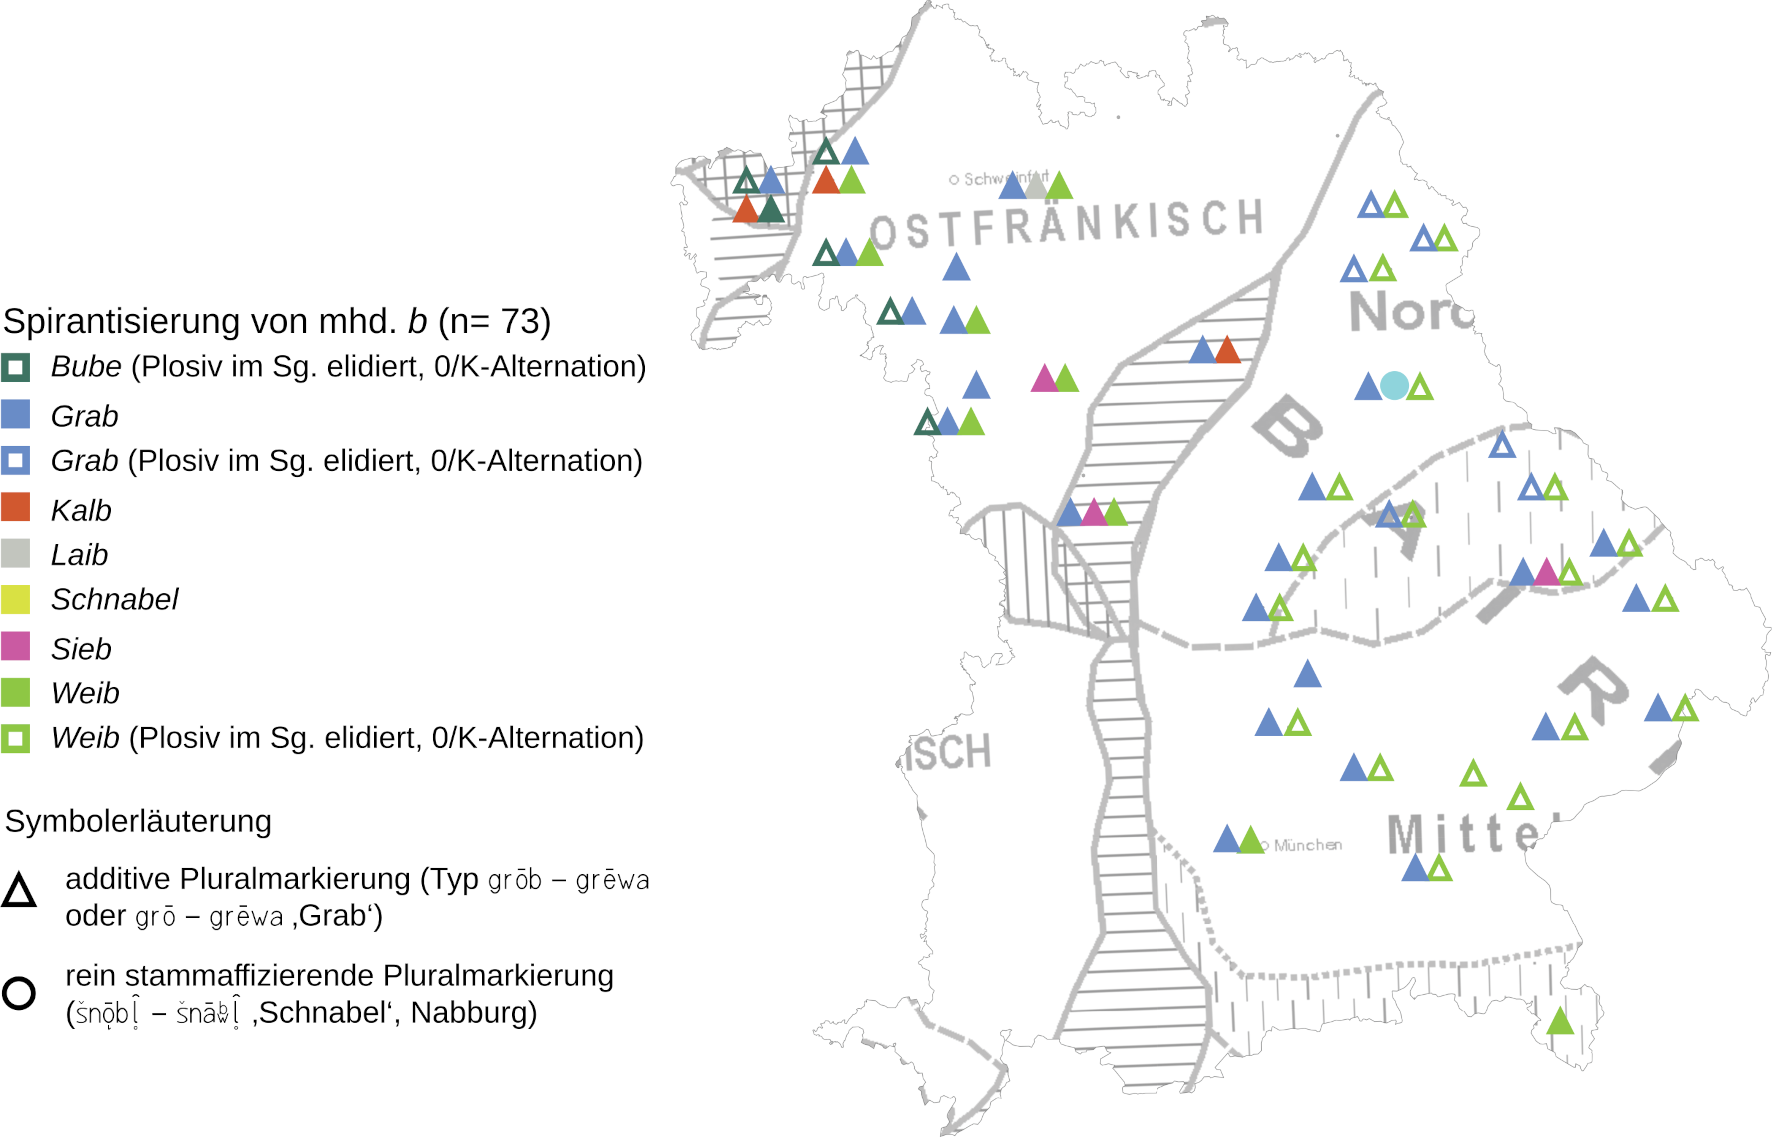
\includegraphics[width=\textwidth]{figures/Karte20.png}
\caption{Spirantisierung von intervokalischem /b/}
\label{map:20}
\end{map}

Spirantisierungen von intervokalischem /b/ in additiven Pluralformen stellen einen Fall kombinatorischer (positionsbedingter) Allophonie dar (vgl. \citealt[125]{Rowley1997}). Anders liegt der Fall bei der Spirantisierung von mhd. \textit{g} und mhd. \textit{c} (aus ahd. \textit{g} in Auslautverhärtung, vgl. \citealt[218--219]{SMF4}), da laut \citet[125]{Rowley1997} die in den Dialekten belegten Minimalpaare die Lösung als Allophonie „verbieten“. Mhd. \textit{g} und mhd. \textit{c} werden im ofr. und nordbair. Teil des UGs je nach Lautumgebung im Inlaut meist spirantisiert, im mittelbair. Teil nicht-spirantisiert (d.\,h. plosivisch) realisiert.\footnote{Im Ofr. erfolgt im In- und Auslaut weitestgehend Zusammenfall, im Nordbair. teilweiser Zusammenfall von mhd. \textit{g} und \textit{ch}, vgl. z.\,B. die Homonymie bei \textit{Tag} und \textit{Dach} in ofr. Erlabrunn (\teuthoo{da2x}{dāx}) und nordbair. Groschlattengrün (\teuthoo{do42X}{dọ̄ꭗ}, vgl. \citealt[Karte 29]{Gütter1971}, \citealt[§29]{Kranzmayer1956}, \citealt[79]{Rowley1997}, \citealt[216--219]{SMF4}, \citealt[241--250]{Steger1968}).} Im gesamten Datenmaterial gibt es nur zwei Belege für die innerparadigmatische Alternation durch Spirantisierung bei mhd. \textit{(c)h}. Im mittelbair. Inning am Holz wird auslautendes [g] in intervokalischer Position zu [x] in spirantisiert: \teuthoo{vu\$rgá\_}{vṳrɡ͈ʰ} -- \teuthoo{vu.yxA4n}{vuͅ⅄xα̣n} ‚Furche‘ (mhd. \textit{vurch}). Diese innerparadigmatische Alternation findet sich vereinzelt auch in umliegenden Ortsdialekten (vgl. \citealt[177 und Karten 40/41]{SNiB7}, \citealt[Karte 86]{SOB4}).\footnote{Auf Alternationen im Konsonantismus wurde bei der Typisierung der Singular- und Pluralformen (respektive der Pluralmarker) in der Auswertung und im Kommentar des SOB nicht eingegangen; die \textit{BayDat}-Vollformen-Karte im REDE-SprachGis zeigt aber, dass es auch hier Alternationen durch Spirantisierung zumindest vereinzelt gibt. Daneben findet sich im ofr.-nordbair. Mitteleschenbach (und bei weiteren Belegen im südlichen ofr.-nordbair. Übergangsgebiet) die innerparadigmatische Alternation zwischen Frikativ im Auslaut und plosivischer Realisierung vor Nasalsuffix bei \teuthoo{h{\textasciitilde}ôe.i.c}{h{\aufstrih}eͅiͅꭗ} -- \teuthoo{he.i.gN}{heͅiͅgŋ} ‚Höhe‘ (mhd. \textit{hœhe}, \textit{hœch}, vgl. \citealt[273]{SMF4}).} 

Spirantisierungen sind als morphophonologische Alternation auf der in der Einführung von \chapref{chap:7} vorgeschlagenen Skala zwischen den Polen lexikalisierte vs. produktive morphophonologische Alternationen zu verorten. Die Spirantisierung von /b/ ist aus synchronen phonologischen Regeln ableitbar und erscheint nur in additiven Pluralformen;\footnote{Die Spirantisierung der einzigen stammaffizierenden Pluralform in \mapref{map:20}, \teuthoo{s\#no.2bl@°}{šnōͅbl̥̑} -- \teuthoo{s\#na2æl@°}{šnā{\burgerbw}l̥̑} ‚Schnabel‘ im nordbair. Nabburg, ist als „Burger“ aus [b] und bilabialem Frikativ [w] im Plural transkribiert. Diese Zwischenwertnotation wurde gemäß den in \sectref{sec:6.3.1.2} dargestellten Typisierungsrichtlinien dem unteren Bestandteil zugeordnet und damit als Spirantisierung annotiert. Ich werte diese Realisierung eher als Beleg der graduellen Realisierung phonetischer Merkmale (hier von Spirantisierung) und weniger als Funktionalisierung als Pluralmarker.} damit liegt kein produktives Kodierungsverfahren vor. Die Spirantisierung von mhd. \textit{(c)h} scheint noch stärker lexikalisiert zu sein. Im Folgenden werden v.\,a. Spirantisierungen von /b/ trotz ihrer phonologischen Bedingtheit als morphologisch relevant berücksichtigt, da die Spirantisierung des Stammauslauts in Pluralformen des Typs \teuthoo{gro2b}{ɡrōb} -- \teuthoo{gre2wA}{ɡrēwα} ‚Grab‘ das folgende Pluralsuffix indiziert. Die Kookkurrenz von Konsonantismusalternation und Pluralsuffix symbolisiert als Ganzes die Pluralinformation, auch wenn es eine „Asymmetrie“ \citep[194]{Ronneberger-Sibold1990} zwischen beiden Einheiten gibt, da die Spirantisierung nicht distinktiv ist (siehe aber \sectref{sec:8.1} zur Konkomitanz von Spirantisierung und Suffix).

Ausgangspunkt dieser Überlegungen ist \citegen[194--201]{Ronneberger-Sibold1990} Modellierung der semiotisch-kommunikativen Rolle des Umlauts und seiner Verselbstständigung als distinktives Zeichen im Laufe des Sprachwandels. Im Falle der Spirantisierung liegt synchron zwar keine „Verselbstständigung“ vor, sie ist in den rezenten Dialekten phonologisch bedingt und damit Begleiterscheinung des Pluralsuffixes, doch ist die semiotische Funktion m.\,E. vergleichbar. Der Vorteil dieser Lösung besteht in meinen Augen darin, dass die phonologische und die morphologische Ebene sowohl in der mentalen Repräsentation als auch in der Perzeption nicht künstlich (nämlich durch ein linguistisches Modell von modularen Ebenen im Sprachsystem) voneinander geschieden werden.

\subsubsection{Subtraktion}
\label{sec:7.1.2.4}
Subtraktive Morphologie besteht in der Kürzung einer Wortform, d.\,h. in der Tilgung von phonologischem Material, um morphologische Information zu kodieren (vgl. \citealt[21]{Birkenes2014}, \citealt[581]{Dressler2000}, \citealt[143]{GolstonWiese1996}). \citet[582]{Dressler2000} versteht unter einer prototypischen Subtraktion „a reductive grammatical morphological process“: Der synchrone morphologische Prozess bestehe in der Reduktion eines Phonems am rechten Rand der Basis, zugleich symbolisiert die Subtraktion als einziger overter Marker eine morphologische Bedeutung (z.\,B. die Pluralinformation). Fälle nicht-prototypischer Subtraktion lassen sich definitorisch weniger eindeutig fassen, sie bestehen beispielsweise in der Reduktion von mehr als einem Phonem oder von weniger als einem Phonem, d.\,h. von einzelnen Phonemmerkmalen, beispielsweise in Form einer Vokalkürzung (bzw. im Schwund einer More, vgl. \citealt[25]{Birkenes2014}, \citealt[582]{Dressler2000}). Ich verwende im Folgenden die enge Definition von (prototypischer) Subtraktion, weshalb Kontraste der Vokalquantität als eigenständige Belege stammaffizierender Morphologie klassifiziert werden (vgl. \sectref{sec:7.1.2.2}).

Ob Singular- und Pluralformen des Typs \teuthoo{khe2nd}{khēnd} -- \teuthoo{khen}{khen} ‚Kind‘ (ofr.-hess. Wiesthal) tatsächlich einen synchronen morphologischen Prozess der Subtraktion im Deutschen und seinen Dialekten belegen, wurde in der Literatur kontrovers diskutiert (vgl. hierzu die Diskussion in \citealt[31--33]{Birkenes2014}). Nach \citet[582]{Dressler2000} setzt die Definition von Subtraktion als morphologischem Prozess „some minimum generality and regularity“ voraus. Letztlich, so \citet[583]{Dressler2000}, hänge der Status der subtraktiven Morphologie in den Dialekten des Deutschen von der Anzahl der involvierten Fälle ab. \citet[23]{Birkenes2014} analysiert subtraktive Formen in den deutschen Dialekten als „weitgehend lexikalisierte morphophonologische Alternationen“ und nicht in dem Sinne als morphologisches Verfahren (vgl. \citealt[184]{Birkenes2014}, \citealt[47]{Haas1988}).

Grundsätzlich setzt \citet[32]{Birkenes2014} folgende zwei phonologischen Entwicklungen an, deren Ergebnis die subtraktiven Plural- und Dativ-Formen sind (vgl. \citealt[47]{Haas1988}, \citealt[14]{Köhler1934}):

\begin{enumerate}[label=(\arabic*)]
\item Aufgrund des Pluralsuffixes steht der stammauslautende Obstruent in den Konsonantenclustern (/nd/, /mb/) bzw. Vokal-Konsonant-Folgen in intervokalischer Position. Er entfällt infolge von Assimilation und Lenisierung, z.\,B. \textit{hɛndə} > *\textit{hɛnə}.
\item Das wortfinale Schwa (und damit die Flexionsendung) wird apokopiert: *\textit{hɛnə} > \textit{hɛn}.
\end{enumerate}

\begin{sloppypar}
Laut \citet[32]{Birkenes2014} ist die Umkehrung der Chronologie der beiden phonologischen Entwicklungen „ausgeschlossen“. Zum einen entfällt der stammauslautende Obstruent in der Nominativ-Singular-Form nicht, zum anderen finden sich nur für jene Substantive subtraktive Formen, die vor Apokope ein Schwa-Suffix in der Nominativ-\slash Akkusativ-Plural- oder Dativ-Singular-Form aufgewiesen haben. Dass subtraktive Formen historisch auf Formen mit Schwa-Reduktionssilbe zurückzuführen sind, stellt dann auch einen zentralen Befund von \citeauthor{Birkenes2014}' (\citeyear{Birkenes2014}) Arbeit dar: „Erst nach der Apokope geht die phonologische Umgebung, in der die Stammtilgung stattgefunden hat, verloren und der Reduktionsprozess wird intransparent“ \citep[33]{Birkenes2014}. Formen des Typs \teuthoo{loAb}{loαb} -- \teuthoo{loi}{loi} ‚Laib‘ im Nordbair. sind gleichermaßen das Ergebnis von Lenisierungen, allerdings treten diese im Kontext der mittelbair. Konsonantenschwächung auch im absoluten Auslaut auf (vgl. \sectref{sec:7.1.2.3.2}). Auch wenn diese Formen formal subtraktiven Formen entsprechen, ist es im Kontext einer dialektgeographischen Darstellung sinnvoll, sie terminologisch (und konzeptuell) zunächst zu unterscheiden und die jeweiligen historischen phonologischen Prozesse zu berücksichtigen.\footnote{Im Rahmen der Datenannotation wurden auf der Ebene der Formenbildung dann auch Subtraktionen und Konsonantismuselisionen unterschieden (zur Klassifikation und Annotation der Deklinationsklassen siehe \sectref{sec:8.1}). Diese Lösung ist primär durch das dialektgeographische Erkenntnisinteresse motiviert, je nach Erkenntnisinteresse kann diese methodische Entscheidung auch anders ausfallen.}
\end{sloppypar}

Dass die diachrone Herleitung und Abgrenzung beider Typen nicht trivial ist, zeigen Belege von (formal) subtraktiven Formen bei \textit{Laib}/\textit{Leib} außerhalb des Bair. \citet[158, FN 6]{GolstonWiese1996} führen für zwei hessische Ortsdialekte die Form \textit{laib} -- \textit{lai} ‚Laib‘ an, die aber nicht den phonologischen Vorkommensbedingungen von subtraktiven Pluralformen entspricht
(\citealt[147]{GolstonWiese1996}). Auch \citet[93--94]{Birkenes2014} analysiert die Tilgung von intervokalischem /b/ in /Vb/-Abfolgen im Osthessischen und Thüringischen nicht als Subtraktionen, sondern als Ergebnis eines Sandhi-Phänomens. Um einen Hiatus zu vermeiden, wird Schwa u.\,a. vor der Präposition \textit{in} getilgt, sodass eine subtraktive Dativ-Singular-Form \textit{läi} ‚Leib‘ erscheint (neben Nom.Sg. \textit{laib} -- Nom.Pl. \textit{lai}, \citealt[350]{Alles1907/1908}, zitiert nach \citealt[94]{Birkenes2014}).

Aus Perspektive einer synchronen Flexionsmorphologie und auch für die mentale Repräsentation ist es auf den ersten Blick unerheblich, wie die nordbair. Pluralform \teuthoo{loAb}{loαb} -- \teuthoo{loi}{loi} und die hess. Form \textit{laib} -- \textit{lai} historisch zu erklären sind, da ihre Struktur in beiden Fällen subtraktiv ist. Doch auch in einer synchronen Flexionsmorphologie sind die beiden Fälle in meinen Augen verschieden zu gewichten, da ein unterschiedliches Verhältnis von Phonologie und Morphologie vorliegt. Die subtraktiven Formen des Hessischen und Thüringischen sind als Folge der Schwa-Apokope im Zuge einer Hiatus-Vermeidung phonologisch bedingt; in der Umgebung vor vokalischem Anlaut führt eine bessere phonologische Struktur zu einer schlechteren morphologischen Struktur (durch Apokope des Schwa-Flexivs des Dat.Sg.).\footnote{Ein Problem bei der Differenzierung der verschiedenen /Vb/-Tilgungen besteht grundsätzlich aber in der Datenlage. \citet[94]{Birkenes2014} führt acht Belege aus dem Thüringischen und Hessischen an, eine abschließende Klassifikation ist daher nur bedingt möglich. Hinzukommt, dass \citet[234]{Alles1907/1908} eine teilweise belegte Übertragung der subtraktiven Dativform in den Nom.Sg. erwähnt; in diesem Fall ist das Phänomen dann wiederum in der Morphologie zu verorten.} Zwar ist auch der nordbair. Typus \teuthoo{loAb}{loαb} -- \teuthoo{loi}{loi} durch phonologische Prozesse entstanden, doch erscheint die Elision hier unabhängig von der phonologischen Umgebung und Sandhi-Effekten; die morphophonologische Alternation ist lexikalisiert. Demgegenüber kann für die hess. und thüring. Dialekte phonologisch bedingte Variation angenommen werden, da die Tilgung (bzw. der Erhalt) des stammauslautenden /b/ je nach phonologischer Umgebung zu erfolgen scheint (vgl. \citealt[94]{Birkenes2014}).

Subtraktion muss des Weiteren von jenen Fällen abgegrenzt werden, in denen die Reduktion in der Opposition zwischen einem vorhandenen vs. einem fehlenden Affix besteht, wie es beispielsweise bei Genitiv-Pluralformen in slawischen Sprachen der Fall ist: russ. \textit{kniga} ‚Buch‘ vs. Gen.Pl. \textit{knig}, tsch. \textit{hodiny} ‚Stunde‘ vs. Gen.Pl. \textit{hodin} (\citealt[25]{Birkenes2014}, \citealt[583]{Dressler2000}). In diesen Fällen gehört das getilgte Element nicht zum Stamm der Nominativ-Singular-Form, sondern entspricht einem Flexionssuffix. Auch in der Form \textit{dona} ‚Frau‘ vs. Nom.Pl. \textit{don}, die \citet[26]{Birkenes2014} für einige norditalienische Dialekte anführt, kann das Fehlen des Affixes in der Pluralform nicht als Beleg eines subtraktiven Verfahrens analysiert werden. Dieses Beispiel entspricht vereinzelten Belegen im BSA-Korpus, bei denen in der Singularform ein vokalisch realisiertes Nasalsuffix erscheint, im Plural hingegen nicht: ofr. \teuthoo{gNi.“A}{ɡŋīͅα} -- \teuthoo{gNi.“}{ɡŋīͅ} ‚Knie‘ (Burgbernheim) und mittelbair. \teuthoo{roAfA}{roαfα} -- \teuthoo{reAf}{reαf} ‚Reif‘ (Pasing).\footnote{\textit{Reifen} wird im UG entweder in der Form \textit{Reif} oder in der Form \textit{Reifen} realisiert. Einzig im ofr. Gebsattel (\teuthoo{ra42v}{rạ̄v} -- \teuthoo{ra42vE}{rạ̄və}), im ofr. Ahorn (\teuthoo{då}{d{\burgeroalpha}} \teuthoo{ghu?md}{ɡhümd} \teuthoo{qA}{ʔα} \teuthoo{re.2v}{rēͅv} \teuthoo{ru?m}{rüm} -- \teuthoo{di}{di} \teuthoo{re.2vm@}{rēͅvm̥}) und im mittelbair. Inning am Holz (\teuthoo{ro4Av5}{rọαv̩} -- \teuthoo{ra4i.fn@}{rạiͅfn̥} neben \teuthoo{re4Av}{rẹαv}) ist Nasalsuffix (bzw. ein vokalisches Suffix) Pluralmarker.} Diese Alternationen sind nicht systematisch, weshalb ich dem Vorschlag von \citeauthor{Dressler2000} (\citeyear[583]{Dressler2000}, ähnlich \citealt[124]{Rowley1997}) folge und sie als (schwache) Suppletion klassifiziere. Als ebenfalls suppletive Pluralformen ordne ich verschiedene Baumbezeichnungen ein, die im ofr. Gemünden am Main als Komposita mit epenthetischem Schwa in der Singularform realisiert wurden: \teuthoo{danEba"(+mE}{danəbã̄\klammerobenpost{}mə} -- \teuthoo{da3nEbo§?4m}{dănəbọ̈̆m} ‚Tanne‘, \teuthoo{biErgEba"(+mE}{biərɡəbã̄\klammerobenpost{}mə} -- \teuthoo{biErgEbo?4m}{biərɡəbọ̈m} ‚Birke‘, \teuthoo{e9.3E.lEba"(+mE}{e\klammeruntenpost{}̆ͅəͅləbã̄\klammerobenpost{}mə} -- \teuthoo{e9.2ElEbo§?4m}{e\klammeruntenpost{}̄ͅələbọ̈̆m} ‚Erle‘, ohne Schwa-Epenthese aber der Simplex \teuthoo{dEr}{dər} \teuthoo{ba"(+m}{bã̄\klammerobenpost{}m} -- \teuthoo{di}{di} \teuthoo{bo§?4m}{bọ̈̆m} ‚Baum‘.\footnote{Vgl. die Form \teuthoo{ba2mE}{bāmə} ‚Baum‘ mit Nullplural bei \citet[21]{Köhler1934}. \citet[91, vgl. Karte 45]{Dietz1954} führt Formen mit epenthetischem Schwa für \teuthoo{ba2mE}{bāmə} ‚Baum‘ in einem Gebiet nördlich von Gemünden am Main an, daneben einen vereinzelten Beleg für die Epenthese bei Sg. \textit{Mann} (\teuthoo{mo.nE}{moͅnə}).} Diese Belege aus Gemünden am Main sind insofern bemerkenswert, als \citet{Köhler1934} in seiner Ortsgrammatik zum Gemündener Stadtteil Aschenroth Belege subtraktiver Pluralformen anführt: \textit{kind} -- \textit{kin} ‚Kind‘, die älteren, gelegentlich vorkommenden Pluralformen \textit{hānd} -- \textit{hen}\footnote{Laut \citet[14]{Köhler1934} ist diese Form nur in dem Sprichwort \textit{filə hen maχə bal ən en} ‚Viele Hände machen bald ein Ende‘ erhalten.} ‚Hand‘ (neben der Form \textit{hend}) und \textit{wānd} -- \textit{wen} ‚Wand‘ (neben \textit{wend}) sowie die Form \textit{lānd} ‚Garten‘ -- \textit{lenər}\footnote{Diese Form würde in der eigenen Analyse nicht als subtraktiver Plural, sondern als additive Pluralmarkierung mit Alternation des Konsonantismus (Plosivelision) klassifiziert werden (vgl. \sectref{sec:7.1.2.3.2}, vgl. \citealt[123--124]{Rowley1997}).} ‚Gartenbeete‘ \citep[14]{Köhler1934} sowie \teuthoo{s\#u2.Eg}{šūͅəɡ} -- \teuthoo{s\#u2}{šū} ‚Schuh‘, \teuthoo{flo.2Eg}{f‌lōͅəɡ} -- \teuthoo{flo?."E}{f‌lȫͅə} ‚Floh‘ \citep[19--20]{Köhler1934}. Hier hat sich Dialektwandel vollzogen, in den Daten der BSA-Erhebung weisen die von Köhler genannten Lexeme keine subtraktive Pluralmarkierung mehr auf: \teuthoo{do.s}{doͅs} \teuthoo{khind\_}{khindʰ} \teuthoo{i.}{iͅ} \teuthoo{gsund5\_}{ɡsund̩ʰ} -- \teuthoo{di}{di} \teuthoo{khinEr}{khinər} \teuthoo{s\#bi“lE}{šbīlə} \teuthoo{i.}{iͅ} \teuthoo{go.AdE}{ɡoͅαdə} ‚Kind‘, \teuthoo{ha"(+nd5\_}{hã̄\klammerobenpost{}nd̩ʰ} -- \teuthoo{he.nd5\_}{heͅnd̩ʰ} ‚Hand‘ und \teuthoo{wa"(+nd5\_}{wã̄\klammerobenpost{}nd̩ʰ} -- \teuthoo{we9.nd5\_}{we\klammeruntenpost{}ͅnd̩ʰ} ‚Wand‘.


\begin{table}
\begin{tabular}{ll}
\lsptoprule
\teuthoo{ha."+nd5\_}{hã̄ͅnd̩ʰ} -- \teuthoo{he.n}{heͅn} & ‚Hand‘\\
\teuthoo{ho4"(+nd}{họ̃̄\klammerobenpost{}nd} -- \teuthoo{ho?n}{hön} & ‚Hund‘\\
\teuthoo{kha."+mb\_}{khã̄ͅmbʰ} -- \teuthoo{khe.m}{kheͅm} & ‚Kamm‘\\
\teuthoo{vlo42gð\_}{vlọ̄ɡ̩ʰ} -- \teuthoo{vlo"?4}{vlọ̈̄} & ‚Floh‘\\
\teuthoo{E}{ə} \teuthoo{gEso94n}{ɡəso\klammeruntenpost{}̣n} \teuthoo{khe"+nd}{khẽ̄nd} -- \teuthoo{di}{di} \teuthoo{khen}{khen} \teuthoo{s\#bi“lE}{šbīlə} \teuthoo{i:m}{i{\doubleogonek}m} \teuthoo{go.<AdE}{ɡôͅαdə} & ‚Kind‘\\
\lspbottomrule
\end{tabular}
\caption{Subtraktive Pluralformen im ofr.-hess. Wiesthal}
\label{tab:38}
\end{table}

Nur in Wiesthal, dem Tiefenbohrungspunkt im ofr.-hess. Übergangsgebiet, lassen sich subtraktive Pluralformen in den BSA-Daten nachweisen (\tabref{tab:38}). Alle fünf Belege weisen im Singular einen stammauslautenden Plosiv auf, der in der Pluralform getilgt ist. Die Pluralformen von \textit{Hand}, \textit{Hund}, \textit{Kamm} und \textit{Floh} weisen neben der Subtraktion weitere stammaffizierende Verfahren in Form von Umlaut und Vokalquantitätskontrast auf. Die Beispiele aus Wiesthal stellen damit keine reine Subtraktion dar -- dies entspräche nach \citet{Dressler2000} dem prototypischen Typus von Subtraktion --, sondern belegen ein subtraktiv-modulatives Verfahren, was im Vergleich zur reinen Subtraktion in Birkenes‘ Korpusstudie das frequentere Pluralmarkierungsverfahren darstellt \citep[47]{Birkenes2014}.

Die phonologischen Umgebungen entsprechen den von \citet[31, 47]{Birkenes2014} beschriebenen: im Stammauslaut /nd/-Konsonantencluster in \textit{Hand}, \textit{Hund} und \textit{Kind} und dem Konsonantencluster /mb/ in \teuthoo{kha."+mb\_}{khã̄ͅmbʰ} ‚Kamm‘. Die Pluralform \teuthoo{vlo42gð\_}{vlọ̄ɡ̩ʰ} -- \teuthoo{vlo"?4}{vlọ̈̄} entspricht nur synchron der Abfolge Vo\-kal+""Kon\-so\-nant /Vg/. Diachron geht das Lexem \textit{Floh} (wie auch \textit{Schuh}) auf einen stimmlosen velaren Frikativ im Mhd. (mhd. \textit{schuoch} und \textit{vlôch}) und im Germ. (germ. \textit{x} aus idg. \textit{k}) zurück (vgl. \citealt[91--93]{Birkenes2014}, \citealt[364--365]{Schirmunski1962}). Während der Frikativ im Auslaut v.\,a. in obd., aber auch in md. Dialekten bewahrt und z.\,T. analogisch auf die intervokalische Position ausgedehnt ist,\footnote{Vgl. die Singular- und Pluralformen \teuthoo{vlôo:<o4X}{vl{\aufstrih}ô{\doubleogonek}ọꭗ} -- \teuthoo{vle<.i.c}{vlêͅiX} ‚Floh‘ in Groschlattengrün und weiteren nord- und mittelbair. Tiefenbohrungspunkten im eigenen Material.} ist (vermutlich seit dem Frühneuhochdeutschen) in den md. (nämlich hess., thüring. und sächs.) Dialekten der Plosiv \textit{k} (\textit{g}) anstelle des Frikativs im Auslaut verbreitet (vgl. \citealt[92]{Birkenes2014}, \citealt[365]{Schirmunski1962}).\footnote{Nach \citet[365]{Schirmunski1962} handelt es sich um eine „Adoption“, die durch Schwankungen in der Realisierung von germ. \textit{g} im Auslaut als Frikativ oder Plosiv begründet ist.} Im Mittelhochdeutschen, so \citet[92]{Birkenes2014}, sei dagegen noch der Frikativ anzunehmen (\textit{schuohe} und \textit{flœhe}), der nach Apokope des Schwa aber entfällt, woraus die synchrone subtraktive Pluralmarkierung \teuthoo{vlo42gð\_}{vlọ̄ɡ̩ʰ} -- \teuthoo{vlo"?4}{vlọ̈̄} im ofr.-hess. Tiefenbohrungspunkt resultiert. Da die Subtraktion bei \textit{Floh} (wie auch \textit{Schuh}) von anderen Fällen des /Vg/-Typs (\textit{Tag}, \textit{Pflug}) zu unterscheiden ist, sei die Subtraktion „in diesem Fall als historischer Zufall einzustufen“ \citep[93]{Birkenes2014}.

\subsection{Null}
\label{sec:7.1.3}
Als Verfahren der Pluralmarkierung umfasst der Nullplural Singular- und Pluralformen, die synchron keine formale Differenzierung aufweisen. Es handelt sich insofern um kein dialektraumspezifisches Verfahren, als synkretische Formen im gesamten UG zu finden sind. Dialektraumspezifisch ist indes der Anteil der Nullmarkierung in den einzelnen Ortsdialekten und die Zusammensetzung der Deklinationsklassen mit Nullmarkierung. \mapref{map:21} illustriert, dass eine Zweiteilung des UGs vorliegt mit einem höheren relativen Anteil im Ofr. und in Teilen des Nordbair. und einem geringeren Anteil von Nullpluralen im südlichen Nordbair., im Mittelbair. sowie den bair. Übergangsgebieten. Im mittelbair.-südbair. Ramsau ist der Anteil synkretischer Singular- und Pluralformen mit 14\,\% am geringsten. Dieser Befund ist auch aus theoretischer Sicht bemerkenswert, da deutlich wird, dass die Dialekte Unterschiede hinsichtlich einer formalen (d.\,h. distinkten) Kodierung der Pluralinformation am Substantiv und Numerussynkretismen aufweisen.


\begin{map}
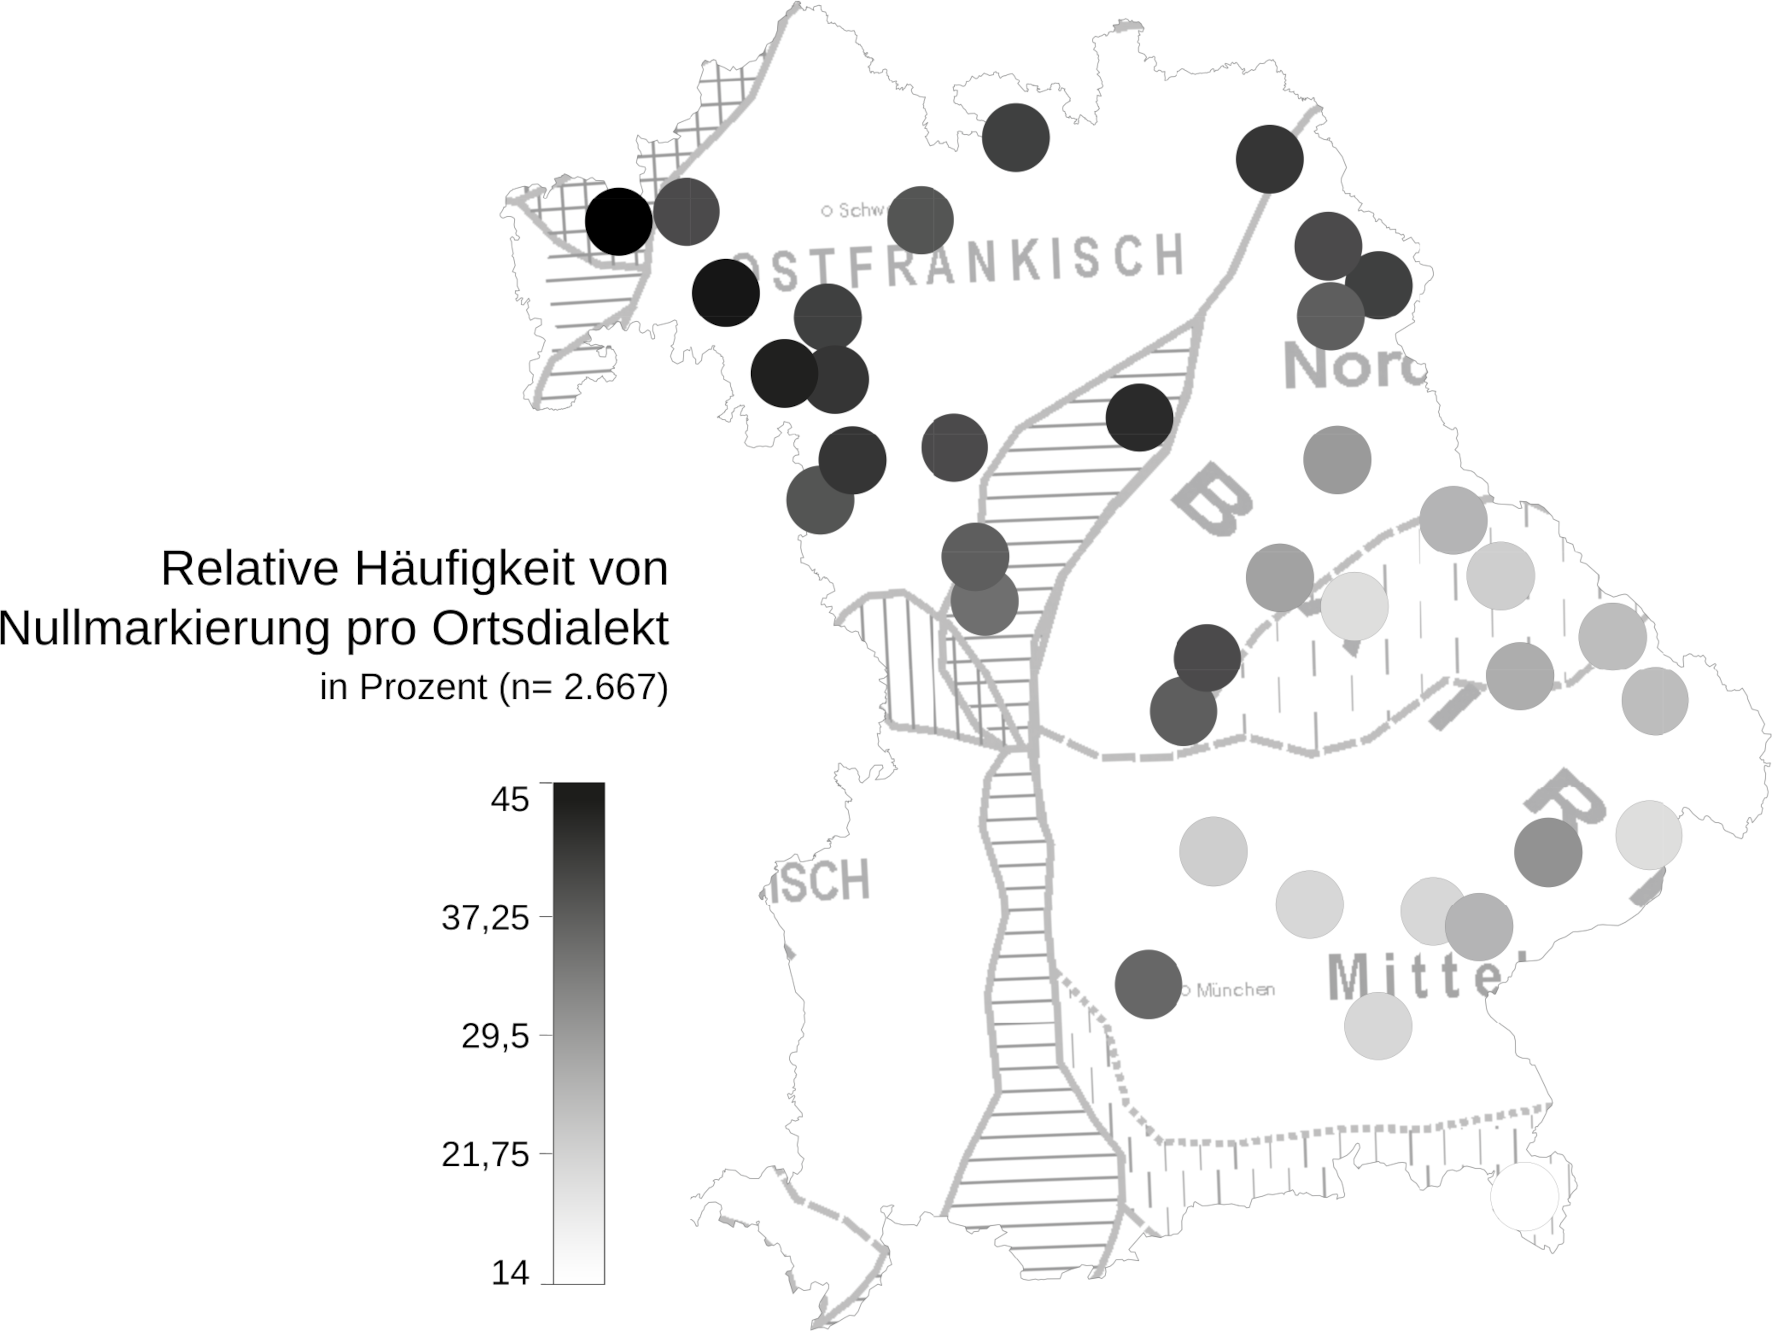
\includegraphics[width=\textwidth]{figures/Karte21.png}
\caption{Chloroplethkarte der relativen Häufigkeit von Nullmarkierung pro Ortsdialekt}
\label{map:21}
\end{map}

Aus diachroner Perspektive und mit Blick auf das historische Deklinationsklassensystem ist Nullmarkierung beispielsweise im Fall der historischen Zweisilber auf -\textit{el}, -\textit{er}, -\textit{en} entweder bereits im Mittelhochdeutschen vorhanden oder als Folge der Apokope des Schwa-Suffixes bei den historischen \textit{a}{}- und \textit{i}{}-Stämmen das Ergebnis eines phonologischen Prozesses (vgl. \sectref{sec:3.1.2}). Der interdialektale Vergleich zwischen Ramsau und (als Beispiel für Dialektsysteme mit einem höheren Anteil von Nullpluralen) dem ofr. Ahorn bestätigt exemplarisch für die mask. \textit{a}{}-Deklination und historische Zweisilber auf -\textit{el}, -\textit{en} den generellen Befund. Beide Substantivklassen weisen im ofr. Ahorn eher Numerussynkretismus auf, während Pluralformen im mittelbair.-südbair. Ramsau durch additive oder stammaffizierende Markierungsstrategien gebildet werden: \teuthoo{dê}{d{\burgereshwa}} \teuthoo{vis\#}{viš} -- \teuthoo{di}{di} \teuthoo{vis\#}{viš} ‚Fisch‘ in Ahorn vs. \teuthoo{vi“s\#5}{vīš̩} -- \teuthoo{viS'}{viʃ̌} in Ramsau, \teuthoo{dAq}{dαʔ} \teuthoo{å>Am}{{\burgerôalpha}αm} -- \teuthoo{di.}{diͅ} \teuthoo{å>Am}{{\burgerôalpha}αm} ‚Arm‘ in Ahorn vs. \teuthoo{o<Åm}{ô{\burgershwaalpha}m} -- \teuthoo{a4m}{ạm} in Ramsau, \teuthoo{A}{α} \teuthoo{ha)\$ovm@}{ha\klammeruntenpost{}̤ovm̥} -- \teuthoo{ha)\$ovm@}{ha\klammeruntenpost{}̤ovm̥} ‚Haufen‘ in Ahorn vs. \teuthoo{ha4<ofn@}{hậofn̥} -- \teuthoo{ha4<i.fn@}{hậiͅfn̥} in Ramsau, \teuthoo{s\#no<8ubl@}{šnô\klammerobenpost{}ubl̥} -- \teuthoo{s\#no<8ubl@}{šnô\klammerobenpost{}ubl̥} ‚Schnabel‘ in Ahorn vs. \teuthoo{s\#no<æi:}{šnô{\burgerbw}i{\doubleogonek}} -- \teuthoo{s\#na4<æen}{šnậ{\burgerbw}en} in Ramsau. Es handelt sich hier aber nur um Tendenzen, auch in Ahorn gibt es Belege für Deklinationsklassenwechsel der mask. \textit{a}{}-Stämme (z.\,B. \teuthoo{dÅ}{d{\burgershwaalpha}} \teuthoo{hu(+nd}{hũ\klammerobenpost{}nd} -- \teuthoo{hu6?nd}{hü̃nd} ‚Hund‘) und in Ramsau Belege für Nullplural (\teuthoo{we94<g@}{we\klammeruntenpost{}̣̂ɡ̥} -- \teuthoo{we94<g}{we\klammeruntenpost{}̣̂ɡ} ‚Weg‘).

Numerussynkretismus und stammaffizierende Markierung können somit die lautgesetzliche Entsprechung der mhd. Flexionsformen sein. In Dialekten mit Lenis-Fortis-Opposition im phonologischen System ist die Pluralvariante \teuthoo{vi“s\#5}{vīš̩} -- \teuthoo{viS'}{viʃ̌} die lautgesetzliche Form, in Dialekten ohne diese Opposition entspricht ihr hingegen die synkretische Form. Inwiefern synchrone Numerussynkretismen oder formale Numerusdifferenzierung für einzelne Substantive oder Substantivgruppen lautgesetzlich entstanden oder das Ergebnis von Deklinationsklassenwechsel sind, wird in Form einer kontrastiven Analyse des historischen und des synchronen Deklinationsklassensystems in \sectref{sec:8.2} behandelt.

\begin{sloppypar}
Daneben kann Numerussynkretismus das Ergebnis von morphologischen „Umschichtungen“ \citep[185]{Rowley1997} im Paradigma sein. Das Flexiv der obliquen Kasusformen oder der Pluralform dringt in die Form des Nom.Sg. ein, in der Folge erscheint Formensynkretismus. Im Falle mhd. schwacher Feminina sowie einiger schwacher Neutra erfolgt die Singularstammbildung durch Nasalsuffix (Typ \teuthoo{mu.gY}{muͅɡ{\klammerNG}} -- \teuthoo{mu.gY}{muͅɡ{\klammerNG}} ‚Mücke‘ im ofr. Burgbernheim, vgl. \sectref{sec:7.1.3.1}), bei einer relativ heterogenen Gruppe an Substantiven durch Umlaut (Typ \teuthoo{dA}{dα} \teuthoo{e?9.b5v5l.}{ë\klammeruntenpost{}ͅb̩v̩lͅ} -- \teuthoo{e?(9.b5v5l@}{ë\klammerobenpost{}\klammeruntenpost{}ͅb̩v̩l̥} ‚Apfel‘ im ofr. Hallerstein, vgl. \sectref{sec:7.1.3.2}).
\end{sloppypar}

\subsubsection{Singularstammbildung mit Nasalsuffix}
\label{sec:7.1.3.1}
Feminina, die synchron eine zweisilbige Struktur mit Reduktionssilbe auf Schwa aufweisen (Type \textit{Brücke}), werden in der Singularform im UG entweder mit apokopiertem Schwa realisiert (\teuthoo{bru.kx}{bruͅkx}, im mittelbair.-südbair. Ramsau) oder weisen Singularstammbildung mit Nasalsuffix auf (\teuthoo{A}{α} \teuthoo{bru?gN@}{brüɡŋ̥} im ofr. Ahorn, vgl. \cites[401]{Rowley1990a}[132--133]{Rowley1997}). Variation besteht in der formalen Realisierung des Nasalsuffixes, in Abhängigkeit vom vorausgehenden Laut wird
{}-\textit{en} zu [m] oder [ŋ] assimiliert oder vokalisch als [ɐ] realisiert (vgl. \sectref{sec:7.1.1.1}). Die \textit{n}{}-Erweiterung stellt dabei ein produktives morphologisches Verfahren der Singularstammbildung dar (z.\,B. \teuthoo{s\#a4tu<i.“4n}{šạtûị̄ͅn}, ‚Schatulle‘ im mittelbair. Neukirchen am Inn oder \textit{loɪb̥m̩} ‚Loipe‘ im Salzburger Lungau, \citealt[132]{Mauser2000}).

In der Literatur gibt es unterschiedliche Herangehensweisen hinsichtlich des Bezugssystems, vor dessen Hintergrund die Beschreibung der Singularstammbildung erfolgt. \citet[186]{Rowley1997} beispielsweise bezieht die Singularstammbildung auf die mhd. Klassen. Diese Lösung wurde mit Blick auf den diachronen Vergleich der Deklinationsklassenzugehörigkeit primär auch für diese Arbeit gewählt, wenngleich es sich um ein Bezugssystem handelt, für das mit Blick auf Pluralmarkierungsverfahren und Singularstammform bereits im Mittelhochdeutschen Variation angenommen werden muss (vgl. \citealt[3--4]{SBS9.1}). In den BSA-Bänden wurde für die nominale Flexionsmorphologie indes grundsätzlich das Neuhochdeutsche als primäres Bezugssystem herangezogen (vgl. \citealt[XXXVI]{SBS9.1}, \citealt[8]{SMF7}). Dies hat für die Singularstammform der Feminina (Apokope vs. \textit{n}{}-Erweiterung) den Vorteil, dass diese nhd. Substantivklasse formal einheitlich ist. \mapref{map:22} (Kartenbild links) zeigt für Feminina dieses Typs und das nhd. Bezugssystem die Häufigkeitsverteilung der Singularstammform im Korpus. Apokopierte und \textit{n}{}-erweiterte Stämme sind im gesamten UG zu finden, allerdings variieren die jeweiligen relativen Anteile. Die Stammbildung mit Nasalsuffix stellt das frequentere Verfahren dar, der Anteil der apokopierten Formen ist in den bair. Dialekten dabei tendenziell höher als im Ofr. Nur im mittelbair. Kirchensur und im mittelbair.-südbair. Ramsau werden die Singularformen mehrheitlich apokopiert realisiert. Gleichzeitig zeigt die Durchsicht sämtlicher Feminina mit \textit{n}{}-Erweiterung, dass diese Form der Singularstammbildung eben nicht nur nhd. zweisilbige Feminina auf Schwa umfasst, sondern ein produktives Verfahren für CVCV-Feminina insgesamt ist.


\begin{map}
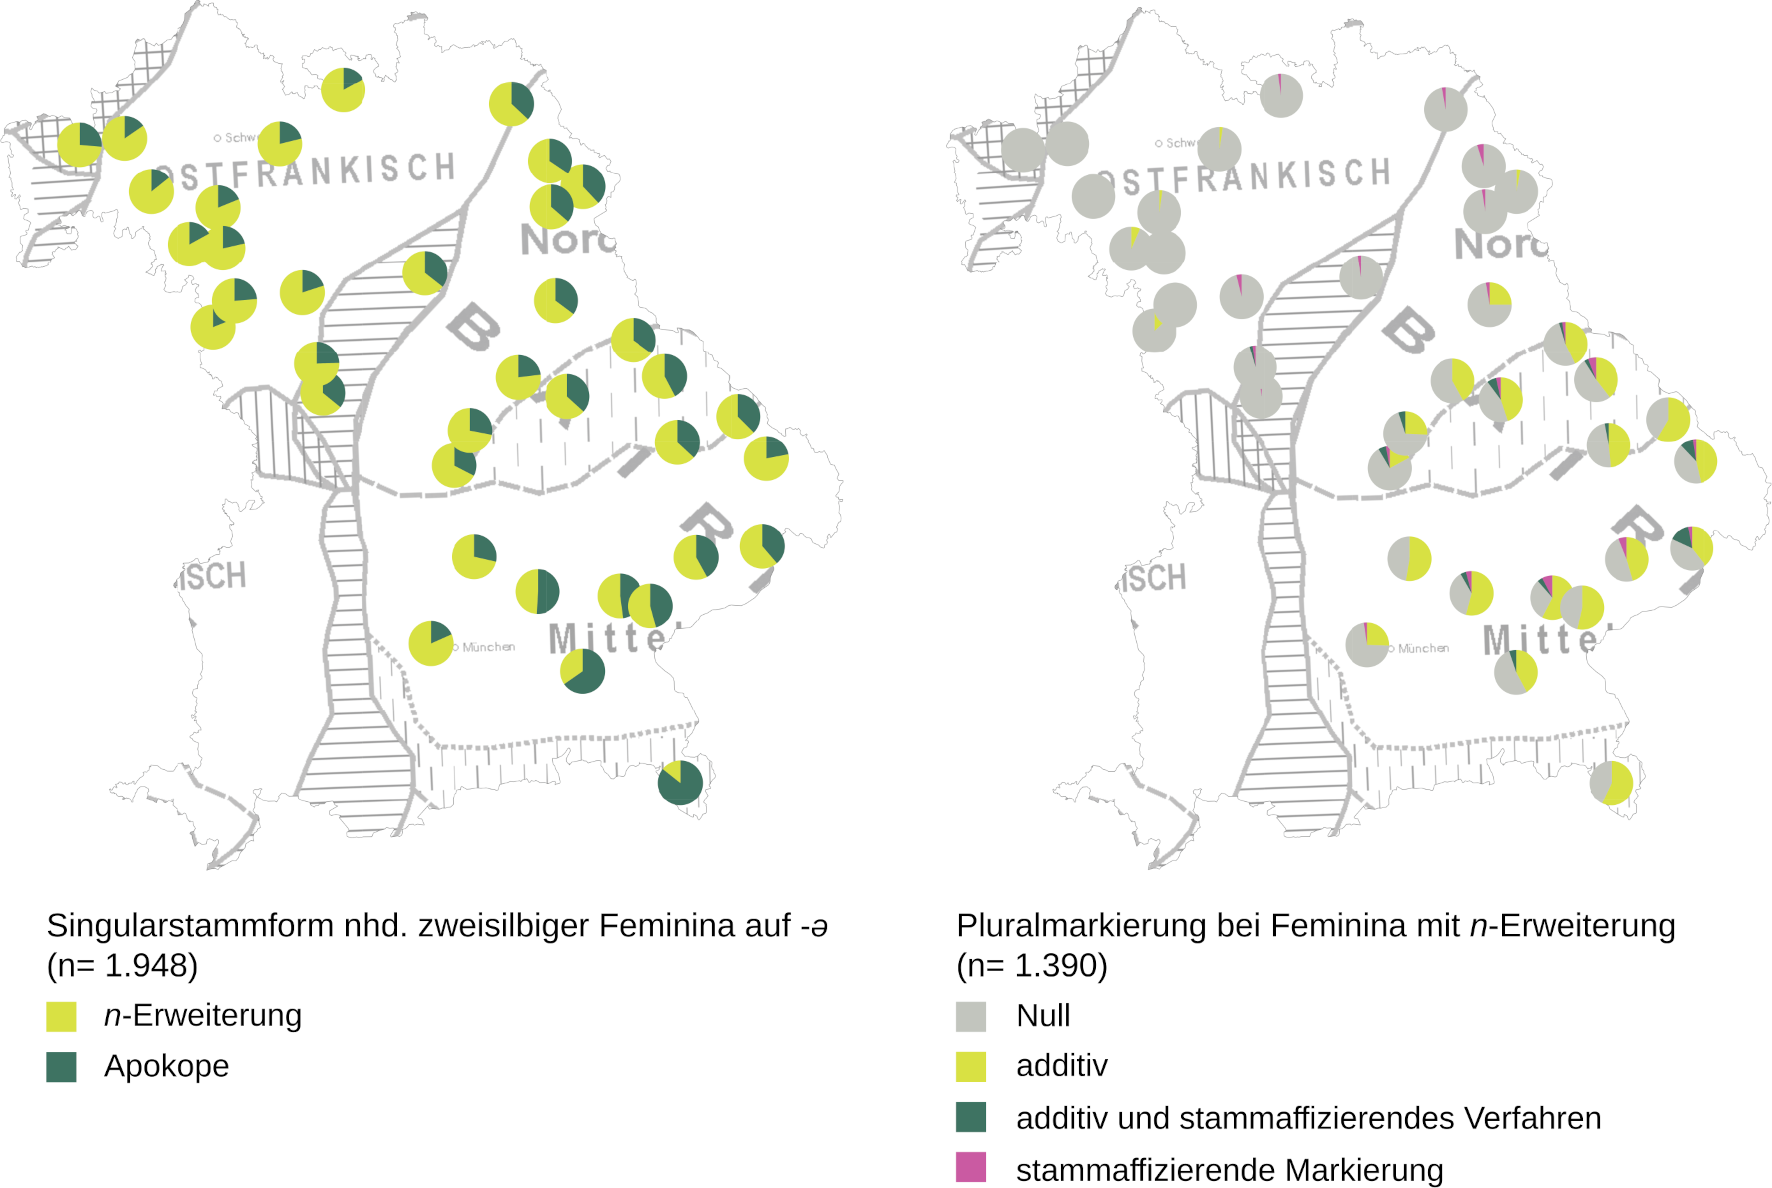
\includegraphics[width=\textwidth]{figures/Karte22.png}
\caption{Singularstammform nhd. zweisilbiger Feminina im Korpus und Häufigkeitsverteilung der Pluraltypen bei \textit{n-}erweiterten Feminina}
\label{map:22}
\end{map}

\begin{sloppypar}
Beide Stammformvarianten sind für die fem. Lexeme im Korpus belegt. Nur in wenigen Fällen findet sich ausschließlich eine der Stammformen, so wird \textit{Katze} nur apokopiert realisiert, \textit{Kette} und \textit{Latte} hingegen nur mit Nasalsuffix. Für das SBS-Arbeitsgebiet wurde die Verteilung von apokopierten vs. nicht-apokopierten Stämmen systematisch untersucht, wobei für die verschiedenen Varianten der Singularform „keine kategorisierenden Kriterien gefunden werden konnten“ (\citealt[147 und Karten 55, 62, 67]{SBS9.1}, vgl. auch \citealt[94]{Merkle1984}). Unter Berücksichtigung der historischen Klassen zeigt \citet[191--192]{Rowley1997} dagegen, dass die synchrone Formenbildung zunächst vor allem die Zugehörigkeit zur schwachen \textit{n}{}- vs. zur starken \textit{ô}{}-Deklination im Mittelhochdeutschen widerspiegelt, auf untergeordneter Ebene kommen dialektspezifisch semantische Aspekte hinzu (siehe hierzu ausführlicher \sectref{sec:8.2.3}).
\end{sloppypar}


\begin{sloppypar}
Die Darstellung der Häufigkeitsverteilung der Pluralmarkierungsstrategien bei sämtlichen \textit{n}{}-erweiterten Feminina in \mapref{map:22} (rechts) zeigt zudem, dass dialektspezifische Unterschiede hinsichtlich der Pluralform bestehen: Im Ofr. und im nördlichen Nordbair. finden sich fast ausschließlich Numerussynkretismen, während im südlichen Nordbair., im Mittelbair. sowie den bair. Übergangsgebieten additive Pluralmarkierung belegt ist und teilweise die frequentere Pluralmarkierungsstrategie darstellt. Hier lohnt es, die Form des Singularstammes neben dem Pluralmarkierungsverfahren als weiteres Merkmal der synchronen Deklinationsklassen heranzuziehen, um (1) den relativen Anteil \textit{n}{}-erweiterter Stämme am Null- bzw. am numerusdistinkten Pluralmarkierungsverfahren und (2) mögliche dialektspezifische Pluralmarkierungsstrategien für diese Struktur des Singularstammes zu ermitteln (Abschnitte~\ref{sec:8.3.1.3} und \ref{sec:8.3.3.1}).
\end{sloppypar}

Daneben findet sich die Generalisierung des Nasalsuffixes bei einigen mhd. his\-to\-risch schwachen und starken Maskulina und Neutra. Im Ofr. sind vereinzelt die Maskulina \textit{Backe,} \textit{Fleck,} \textit{Ochse} und \textit{Spatz} belegt,\footnote{\textit{Backe} und \textit{Fleck} wurden nur im SMF-Teilprojekt in der Singular- und Pluralform abgefragt.} in den bair. Dialekten finden sich die Neutra \textit{Auge}, \textit{Ohr} und das Maskulinum \textit{Hachse} (vgl. \citealt[§137]{Kollmer1987}, \citealt[8--9]{Mausser1915}, \citealt[190]{Rowley1997}, \citealt[121]{Steininger1994}, \citealt[147]{Wildfeuer2001}).

\subsubsection{Singularstammbildung mit Umlaut}
\label{sec:7.1.3.2}
Im gesamten UG (mit Ausnahme des ofr.-hess. Wiesthal, des mittelbair. Pasing und des mittelbair.-südbair. Ramsau) erscheinen die mhd. starken Feminina \textit{Bank}, \textit{Hand} und \textit{Wand} mit dem Umlaut des mhd. Pluralparadigmas bzw. der Obliquusformen des Singularparadigmas in der Nominativ-Singular-Form, z.\,B. \teuthoo{b5e.Nk\_}{b̩eͅŋkʰ} -- \teuthoo{b5e.Nk\_}{b̩eͅŋkʰ} ‚Bank‘ im nordbair. Groschlattengrün, \teuthoo{ve4nd}{vẹnd} -- \teuthoo{ve4nd}{vẹnd} ‚Wand‘ im ofr. Burgbernheim (vgl. \citealt[54]{Roth1940}, \citealt[190]{Rowley1997}, \citealt[443]{Schirmunski1962}, \citealt[§803]{Schmeller1821}).\footnote{\citet[325]{Schiepek1908} führt für das nordbair. Egerland außerdem noch die synkretischen Singular- und Pluralformen bei den Feminina \textit{Bráit} ‚Braut‘, \textit{Néit} ‚Nute‘ und \textit{Háit} ‚Haut‘ sowie \textit{Áks} (mit Umlaut) ‚Achse‘ u.a. an. Vgl. zudem die Darstellung in den Dialektgrammatiken von \citet[31]{Förster1912/13}, \citet[86]{Kemmeter1924}, \citet[285--284]{Schübel1955}.}  Da im Bair. -- laut \citet[331]{Zehetner1983} im „ländlichen Dialekt“ -- auch die Fortiskonsonanz des Plurals in den Singular eingedrungen ist, ist in den Singularformen der bair. Untersuchungsorte (nicht aber in der Diminutivform) teilweise neben Umlaut auch Fortiskonsonanz zu finden, z.\,B. \teuthoo{he.nt\_}{heͅntʰ} -- \teuthoo{he.nt\_}{heͅntʰ} --Dim. \teuthoo{he.nd5Al}{heͅnd̩αl} ‚Hand‘ im nordbair.-mittelbair. Blaibach. Im ofr.-hess./ofr.-rheinfränk. Teil des UGs, in dem subtraktive Formen belegt sind, sind die Subtraktionen der Pluralform auch in der Singularform zu finden, z.\,B. \teuthoo{hen}{hen} -- \teuthoo{di}{di} \teuthoo{hen}{hen} -- Dim. \teuthoo{henHEn}{henhͯən} ‚Hand‘ im ofr.-hess. Straßbessenbach (vgl. \citealt[12]{Hirsch1958}). Infolge des Eindringens der Pluralflexive in den Nom.Sg. weisen Singular- und Pluralformen keine Numerusdifferenzierung auf, allerdings sind großräumig \textit{Wand} und z.\,T. \textit{Bank} im Bair. und vereinzelt auch im Ofr. mit additiver Pluralmarkierung belegt, z.\,B. \teuthoo{be.Nk\_}{beͅŋkʰ} -- \teuthoo{be.NgN}{beͅŋɡŋ} ‚Bank‘ im ofr.-nordbair. Pfofeld, \teuthoo{we4nt}{wẹnt} -- \teuthoo{dwe4ntn@}{dwẹntn̥} ‚Wand‘ im nordbair. Kallmünz (vgl. \sectref{sec:8.2.3}).


\begin{map}
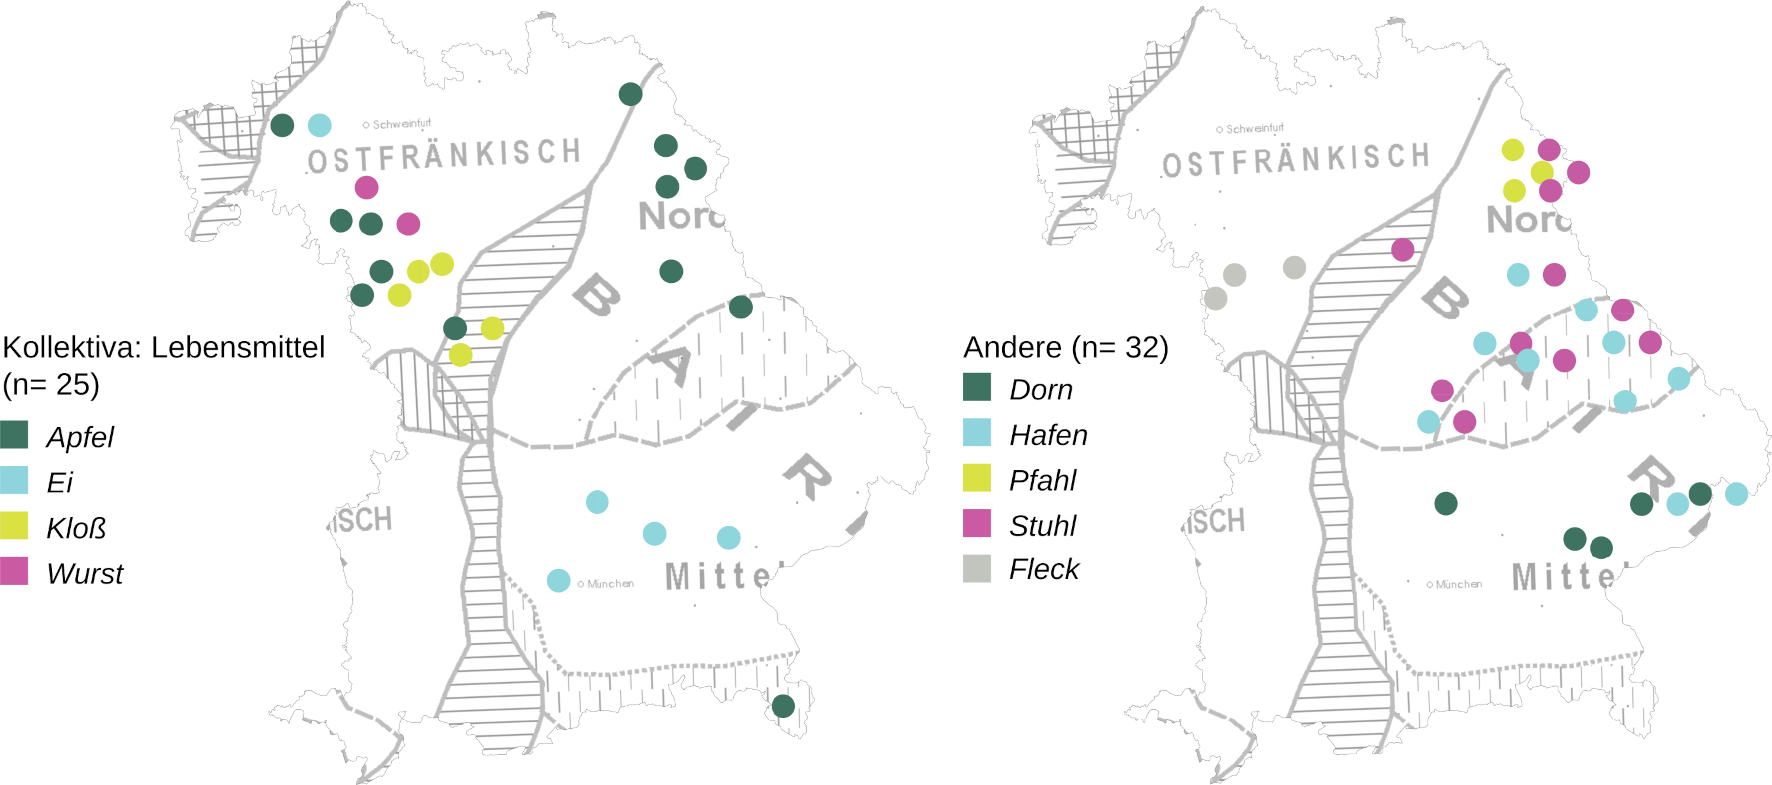
\includegraphics[width=\textwidth]{figures/Karte23.png}
\caption{Areale Verteilung von sogenannten Markiertheitsumkehrungen}
\label{map:23}
\end{map}

\citet[190]{Rowley1997} argumentiert, dass \textit{Bank}, \textit{Hand} und \textit{Wand} typischerweise in Lokativphrasen vorkommen („auf der Bank, an der Wand, in der Hand“), was zu einer „Primärspeicherung“ der Obliquusformen und in der Folge zu einer Generalisierung des Umlauts im gesamten Singularparadigma geführt haben kann (vgl. \citealt[54]{Roth1940}, \citealt[843]{Tiersma1982}). Zudem gehört \textit{Hand} zur semantischen Gruppe der paarigen Körperteile, in der auch die Neutra \textit{Auge} und \textit{Ohr} Numerussynkretismen aufweisen (vgl. \sectref{sec:8.3.2.1}). Das Vorkommen in Menge und damit die höhere Vorkommensfrequenz der Pluralform kann auch das Eindringen des Umlauts in die Singularform bei einer relativ heterogenen Gruppe an Substantiven erklären, die durch weitere Belege in Dialektgrammatiken noch ergänzt werden kann: die Lebensmittel \textit{Apfel}, \textit{Kloß}, \textit{Wurst}, daneben \textit{Dorn}, \textit{Hafen}, \textit{Pfahl} und \textit{Stuhl}\footnote{Vgl. \citet[Karte 99]{Brendel1962}.} sowie -- als Einzelbelege -- \textit{Bloch}, \textit{Darm}, \textit{Floh}, \textit{Furche}, \textit{Turm}, \textit{Zopf} (vgl. \citealt[189]{Rowley1997}, \citealt[324--325]{Schiepek1908}, \citealt[442--443]{Schirmunski1962}). \mapref{map:23} illustriert, dass die einzelnen Fälle teilweise für einzelne oder mehrere Dialekträume belegt sind, z.\,T. aber auch nur einem kleinen Gebiet vorkommen.

Ausgehend von ihrer Semantik und Gebrauchsfrequenz kann das Eindringen des Umlauts der Pluralform (im Fall von \textit{Ei} ist es das Eindringen des \textit{r}-Suffixes) in die Singularform als sogenannte Markiertheitsumkehrung im Sinne \citegen[48--58]{Mayerthaler1981} klassifiziert werden: Die Pluralform ist die frequentere und damit unmarkierte Form (ausführlicher hierzu \citealt{Bybee2010}). Wie bei den starken Feminina \textit{Wand} und \textit{Bank} finden sich auch hier neben Numerussynkretismen als Normalfall Belege für formale Numerusdifferenzierung wie die additive Markierung von \teuthoo{de.2n}{dēͅn} -- \teuthoo{de.2nA}{dēͅnα} ‚Dorn‘ im mittelbair. Wolfersdorf und \teuthoo{s\#dôe{\textasciitilde}îl}{šd{\aufstrih}e{\aufstrih}l}
 -- \teuthoo{s\#dôe{\textasciitilde}îln@}{šd{\aufstrih}e{\aufstrih}ln̥} ‚Stuhl‘ im nordbair.-mittelbair. Blaibach oder die stammaffizierende Form \teuthoo{he42vA}{hẹ̄vα} -- \teuthoo{the4vA}{thẹvα} ‚Hafen‘ im nordbair.-mittelbair. Grafenkirchen. Bemerkenswert ist hier die Form \teuthoo{dsi.“bv5}{dsīͅbv̩} (neben \teuthoo{dse\$2bv}{dsē̤bv}) ‚Zopf‘-- \teuthoo{di}{di} \teuthoo{la.NE}{laͅŋə} \teuthoo{dse4bv}{dsẹbv} ‚die langen Zöpfe‘ im ofr.-hess. Wiesthal.: Der innerparadigmatische Wechsel der Zungenhöhe zwischen \teuthoo{i.“}{īͅ} und \teuthoo{e.}{eͅ} ist historisch aus der Hebung von mhd. \textit{ö} in Dehnung in der Singularform und mhd. \textit{ö} in der Pluralform in Normalentwicklung entstanden (vgl. \sectref{sec:7.1.2.1.1}). Das Eindringen des Umlauts in die Singularform ist damit älter als die phonologischen Prozesse Einsilberdehnung und Hebung von mhd. \textit{ö}.

\subsection{Suppletion}
\label{sec:7.1.4}
Synchron ist eine Form dann suppletiv, „wenn sie nicht nach allgemeinen phonologischen oder morphologischen Regeln abgeleitet werden kann“ \citep[78]{Nübling1999}. \citet{Melcuk2000} fokussiert in seinem Überblicksartikel zur Suppletion zugleich den relationalen Charakter des Phänomens. Suppletiv ist weder eine linguistische Einheit noch eine linguistische Operation, sondern Suppletion beschreibt eine binäre Beziehung zwischen zwei sprachlichen Zeichen X und Y („X is suppletive with respect to Y“, \citealt[510]{Melcuk2000}). Im Bereich der Flexionsmorphologie wird Suppletion als „Extremfall von Irregularität“ \citep[77]{Nübling1999}, als „Störungen des grundlegenden Uniformitätsprinzips ‚eine Bedeutung -- eine Form‘“ häufig als marginales Phänomen behandelt und dargestellt. Forschung zu suppletiven Flexionsformen in der Standardsprache und zur diachronen Herausbildung suppletiver Formen in verschiedenen Sprachen zeigt indes, dass (1) Suppletion und eine hohe Gebrauchsfrequenz korrelieren und (2) suppletive Formen tendenziell kurz und komprimiert sind, was aus sprachökonomischer Perspektive einen Vorteil im Bereich der Performanz bedeutet (vgl. \citealt{Nübling1999}, \citealt{Plank1981}, \citealt{Ronneberger-Sibold1988}). Suppletion stellt dabei ein graduelles Phänomen dar (vgl. \citealt[514--515 und 517--519]{Melcuk2000}, \citealt[30]{Plank1981}, \citealt[129]{Rowley1997}). Hinsichtlich der Ähnlichkeit zwischen zwei Formen wird zwischen den Polen starke Suppletion (keine formale Ähnlichkeit) und schwache Suppletion (Teilähnlichkeiten) unterschieden.\footnote{\citet[517--518]{Melcuk2000} unterscheidet neben der Gradualität hinsichtlich der formalen Ähnlichkeit auch Gra\-dualität hinsichtlich der Regularität der semantischen Beziehung zwischen X und Y (flexivische Suppletion als semantisch stark, derivationelle Suppletion als semantisch schwach).}

Um Suppletion im Bereich der dialektalen Flexionsmorphologie adäquat erfassen und klassifizieren zu können, muss ein Aspekt fokussiert werden, der sich aus der oben genannten synchronen Minimaldefinition von Suppletion ergibt: Inwiefern kann eine über den Einzelfall hinausgehende allgemeine phonologische oder morphologische Regel formuliert werden? Als suppletiv behandelt beispielsweise \citet[129, 166]{Rowley1997} Pluralformen, die sich zwar mithilfe formaler Marker und flexivischer Prozesse beschreiben lassen, die aber mit Blick auf die Typenfrequenz Einzelfälle darstellen. Als suppletiv zu klassifizieren wären demnach isolierte Fälle von Quantitätskontrasten oder Konsonantismusalternationen (vgl. \citealt[124, 165]{Rowley1997}) respektive von Subtraktion \citep[583]{Dressler2000}; den Referenzpunkt bildet hier das jeweilige Dialektsystem. Lassen sich innerparadigmatische Alternationen hingegen „in eine stärker besetzte Modifikation“ (wie etwa den Diphthongwechsel bei mhd. \textit{ei}) einordnen, handele es sich nicht um Suppletion, sondern um ein eigenes Flexionsmuster \citep[129]{Rowley1997}. \citet[78]{Nübling1999} unterscheidet daneben suppletive Flexionsformen, bei denen ein reguläres Flexiv an die suppletive Wurzel tritt: Durch das segmentierbare Flexiv ist die gesamte Wortform „etwas weniger suppletiv“ als eine suppletive Wortform ohne Flexiv.

Insgesamt ist die Klassifikation von Suppletion damit in vielen Fällen eine Frage der Abwägung und letztlich auch der Granularität des Datenmaterials. Um festzustellen, ob eine irreguläre Pluralform tatsächlich einen isolierten Beleg darstellt und damit möglicherweise als suppletiv zu klassifizieren ist, braucht es ein ausreichend dichtes Ortsnetz und ein entsprechendes Korpus erhobener Flexionsformen. Vor dem Hintergrund der Zusammensetzung des BSA-Korpus, des interdialektalen Vergleichs der Formenbildung und der Typenfrequenz im gesamten Korpus wurden 78 Belege als suppletiv klassifiziert. Als schwächere Formen von Suppletion wurden klassifiziert:

\begin{itemize}\sloppy
\item reduzierte Formen des Lexems \textit{Gemeinde} im Singular, nicht-reduzierte Form im Plural ($n=16$), z.\,B. \teuthoo{gma42}{ɡmạ̄} -- \teuthoo{gEma4<e\$ndn@}{ɡəmậe̤ndn̥} (ofr. Burgbernheim)
\item reduzierte Formen des Kompositums \textit{Werktag} im Singular, nicht-reduzierte Form im Plural ($n=2$): \teuthoo{we94<ArE}{we\klammeruntenpost{}̣̂αrə} -- \teuthoo{weAgát;a42g}{weαɡ͈t͓͓ạ̄ɡ} (mittelbair. Neukirchen am Inn), \teuthoo{we9.<AdE}{we\klammeruntenpost{}̂ͅαdə} -- \teuthoo{we.Agt,o.g\_}{weͅαɡt͓oͅɡʰ} (mittelbair. Inning am Holz)
\item Variation in der Singular- und Pluralform zwischen den Wortstämmen \textit{Huhn} und \textit{Henne} ($n=2$, vgl. \citealt[129]{Rowley1997}): \teuthoo{he9.nA}{he\klammeruntenpost{}ͅnα} -- \teuthoo{hu§?nê}{hü̆n{\burgereshwa}} (ofr. Ahorn), \teuthoo{hena}{hena} -- \teuthoo{hi.“nEr}{hīͅnər} (ofr. Hallerstein)
\item Variation in der Singular- und Pluralform zwischen dem Simplex \textit{Breite} und der derivierten Form \textit{Breiting} ($n=2$): \teuthoo{A}{α} \teuthoo{b5ro9.2AdA2}{b̩ro\klammeruntenpost{}̄ͅαdᾱ} -- \teuthoo{b5ro9.2Adi:NA}{b̩ro\klammeruntenpost{}̄ͅαdi{\doubleogonek}ŋα} (nordbair.-mittelbair. Bernried), \teuthoo{bra42de4N}{brạ̄dẹŋ} -- \teuthoo{bra42d,E}{brạ̄d͓ə} (ofr.-hess. Wiesthal)
\item die in \sectref{sec:7.1.2.4} beschriebenen Fälle nicht-systematischer Subtraktion ($n=5$).
\end{itemize}

Starke Suppletion liegt vor, wenn die Pluralformen außerflexivisch realisiert wurden:

\begin{itemize}
\item Die Pluralform ist durch eine Wortbildung bzw. ein anderes Lexem realisiert ($n=9$), v.\,a. Frauenbezeichnungen wie \teuthoo{b5a42i.E@re\$}{b̩ạ̄iͅə̥re̤} -- \teuthoo{b5a42o4Enwa42i.BA.}{b̩ạ̄ọənwạ̄iͅ{\btilde}ᾳ} (nordbair. Groschlattengrün)\footnote{Im Nordbair. des Egerlandes weicht man \citet[320]{Schiepek1908} zufolge den Pluralformen movierter Feminina „gerne aus“, indem Komposita mit „-mädchen“ (\textit{Wéschəmài(d)lə} ‚Wäscherinnen‘) und „-weiber“ bildet, Formen wie \textit{Wéschərinnən} fänden sich „in der Stadt“.} und \teuthoo{ba<uEs\#vra.2}{bâuəšvrāͅ} -- \teuthoo{ba<u.Es\#wo.2iwE.}{bâuͅəšwōͅiwəͅ} ‚Bäuerin‘ (ofr.-hess. Wiesthal) und \teuthoo{va4<e\$b}{vậe̤b} -- \teuthoo{va4<e\$sbîi.“4l.dA}{vậe̤sb{\aufstrih}ị̄ͅlͅdα} ‚Weib‘ (ofr. Mitteleschenbach), daneben \teuthoo{sqo\$2A2}{sʔō̤ᾱ} -- \teuthoo{dqo\$2A2nwa4s\#\%l@}{dʔō̤ᾱnwạš͈l̥} ‚Ohr‘ (nordbair.-mittelbair. Bernhardswald) und \teuthoo{do.X2}{doͅꭗ̄} -- \teuthoo{da4xAra4<i:"}{dạxαrậī{\doubleogonek}} ‚Dach‘ (mittelbair. Inning am Holz), wobei die formale Ähnlichkeit zwischen Singular- und Pluralform von Fall zu Fall stärker oder schwächer ausfällt.
\item Die Pluralform ist als Diminutivform realisiert ($n=29$), z.\,B. \teuthoo{glo<s}{ɡlôs} -- \teuthoo{gla4<sl@}{ɡlậsl̥} ‚Glas‘ (mittelbair. Grafenau). Mehrfach belegt ist dieser Typ der starken Suppletion für die Lexeme \textit{Bach}, \textit{Brücke}, \textit{Draht}, \textit{Fest}, \textit{Glas}, \textit{Kalb}, \textit{Rad}.
\item Die Singularform ist als Diminutiv realisiert, die Pluralform als flektierte Form des Simplex ($n=10$), z.\,B. \teuthoo{mu.gáAl}{muͅɡ͈αl} -- \teuthoo{b5mu.gð-N@}{b̩muͅɡ̩{}͐ŋ̥} ‚Mücke‘ (nordbair.-mittelbair. Bernried).
\end{itemize}

Aufschlussreich sind hier die Fälle intra-individueller Variation und die vereinzelten Kommentare der Gewährspersonen im Datenmaterial. So hat die Gewährsperson im ofr. Burgbernheim die Pluralformen \teuthoo{v5e9.sd5\_}{v̩e\klammeruntenpost{}ͅsd̩ʰ} -- \teuthoo{v5e9.sdJi.}{v̩e\klammeruntenpost{}ͅsd{\lkreis}iͅ} neben der Form \teuthoo{v5e9.sdEr}{v̩e\klammeruntenpost{}ͅsdər} ‚Fest‘, \teuthoo{dra.2d5\_}{drāͅd̩ʰ} -- \teuthoo{dre.2dli.}{drēͅdliͅ} neben der Form \teuthoo{dre.2d5\_}{drēͅd̩ʰ} realisiert und die Diminutivformen jeweils mit „das ist die Mehrzahl“ kommentiert. Die Gewährsperson im ebenfalls ofr. Gebsattel hingegen hat die Pluralformen \teuthoo{k\_alb}{kʰalb} -- \teuthoo{k\_e.lBli.}{kʰeͅl{\btilde}liͅ} ‚Kalb‘, \teuthoo{bo.2x}{bōͅx} -- \teuthoo{be.Xli.}{beͅꭗliͅ} ‚Bach‘ gebildet und die suggerierten flektierten Simplexformen abgelehnt (vgl. \citealt[29]{SMF7}). Dass die Diminutivform damit eine reguläre, flexivische Pluralform zumindest in diesen (lexemspezifischen) Fällen ersetzen kann, legen die Gewährspersonenkommentare nahe und auch, dass es tendenziell die gleichen Substantive im Datenmaterial sind, deren Pluralform in Form eines Diminutivs gebildet werden. Interessant ist hier auch die Einschätzung im SMF: Die flexivischen Pluralformen sind „von den GPs [Gewährspersonen, GN] ganz eindeutig konstruiert und sind wohl in der entsprechenden Grundma. [Grundmundart, GN] nicht geläufig“, es bestehen „ohne Arealbildung gewisse Schwierigkeiten mit der Kategorie Plural“ (\citealt[29]{SMF7}). Suppletive Formen finden sich dabei vor allem im psychischen Nah- und „‚unmittelbaren Erfahrungsbereich‘ der Sprecher“ (\citealt[57]{Harnisch1990}, vgl. \citealt[520]{Melcuk2000}).

\section{Kasusmarkierung im UG}
\label{sec:7.2}
Dialektale Kasusmarkierung findet an der Schnittstelle von Morphologie und Syntax statt. Diachron ist die Markierung der Kasusinformation am Substantiv in den untersuchten Dialekten weitestgehend abgebaut worden, sodass die Singular- und Plural-Kasusparadigmen mehr oder weniger aus synkretischen Formen bestehen. In den Dialekten des UGs findet damit eine Entwicklung der Deflexion der Kasusinformation am Substantiv statt, die in den Dialekten des Deutschen insgesamt, aber auch für die Standardsprache belegt ist (vgl. \chapref{chap:4}). Gleichzeitig finden sich auch im Bereich der Kasusflexion dialektraumspezifische, nämlich v.\,a. nordbair. Markierungsstrategien im Dat.Pl. neben einem uniformen Nasalsuffix der obliquen Kasusformen (\sectref{sec:7.2.1}). In \sectref{sec:7.2.2} werden die verschiedenen Konstellationen von distinkten vs. synkretischen Formen im Kasusparadigma behandelt, die sich in den untersuchten Dialekten nachweisen lassen. Da dabei nicht nur die Formenbildung des Substantivs, sondern auch die der Substantivbegleiter relevant ist, wird hier immer wieder ein Vorgriff auf die Morphosyntax der Nominalphrase notwendig sein, die systematisch erst in \chapref{chap:9} dargestellt wird.\largerpage

\begin{sloppypar}
Die Auswertung der Kasusbildung erfolgt auch hier in der Word-and-par\-a\-digm-Per\-spek\-ti\-ve. Aus methodischen Gründen bilden zunächst die standardsprachlichen Abfrage-Items im Akkusativ oder Dativ des BSA-Fragebuchs den Referenzpunkt. Von den insgesamt 8.129 Singular- und Pluralformen im Nominativ sind 700 Items auch im Akkusativ und 761 Items im Dativ belegt (1.461 Kasusformen insgesamt). Für 179 Datensätze liegen sowohl Dativ- als auch Akkusativ-Items vor. Damit ist der Anteil der Substantive, für die ein Flexionsparadigma zumindest in Teilen aufgestellt werden kann, ausgesprochen gering. Zugleich variiert die Gewichtung der syntaktischen Funktionen und morphosyntaktischen Kontexte, die für die einzelnen Kasus abgefragt wurden. Erhoben wurden 29 Formen im Akk.Sg. (hiervon 11 historisch schwache Substantive\footnote{\textit{Backe}, \textit{Bauer}, \textit{Bube}, \textit{Hase}, \textit{Hecht}, \textit{Karpfen}, \textit{Ochse}, \textit{Rabe}, \textit{Spatz}, \textit{Specht} und \textit{Zecke}.} sowie 4 Präpositionalphrasen) und 8 im Akk.Pl., 14 Formen im Dat.Sg. (davon 13 Präpositionalphrasen) sowie 19 im Dat.Pl. (13 Präpositionalphrasen).\footnote{Gezählt und ausgewertet wurden hier nur jene Frage-Items, für die auch eine Nominativ-Singular- und/oder
{}-Pluralform erhoben wurde.}
\end{sloppypar}

\begin{sloppypar}
Idealiter sollte sich die Analyse der dialektalen Kasusrelationen bottom-up ausgehend von den syntaktischen Funktionen, tatsächlich realisierten Flexionsformen und der Rektion durch Präpositionen und Verben ergeben. Dies ist dann nicht möglich, wenn Kasusformen nur als isolierte Formen und ohne weiteren morphosyntaktischen Kontext erhoben oder trans\-kri\-biert wurden. In diesen Fällen erfolgt die Analyse nur top-down ausgehend vom BSA-Fragebuch, d.\,h. über die schriftsprachliche Kasusmorphologie und syntaktischen Funktionen, ggf. über die Verb\-va\-lenz. Auch hinsichtlich der formalen Variation in den Daten ist es bedauerlich, dass von den abgefragten Syntagmen bisweilen nur jene Teile trans\-kri\-biert wurden, die für den zu erhebenden Phänomenbereich relevant waren -- wenngleich dies mit Blick auf das extensive Fragebuch und die Erhebungspraxis verständlich ist.
\end{sloppypar}

Vor allem vor dem Hintergrund einer Klassifikation morphophonologischer Markierungsstrategien zeigen die Fälle von formaler Variation, die zwischen einzelnen Formen im Paradigma zu finden sind, wie schwierig die Abgrenzung von phonetisch-phonologisch bedingten (und eventuell auch freien) Alternationen und morphophonologisch funktionalisierten Alternationen ist. So bleibt offen, in welchem Umfang Sandhi-Effekte die innerparadigmatische Alternation von erhaltenem und elidiertem Konsonanten beeinflussen, z.\,B. Nom.Sg. \teuthoo{s\#do942d\_}{šdo\klammeruntenpost{}̣̄dʰ} ‚Stadt‘ -- Akk.Sg. \teuthoo{i.}{iͅ} \teuthoo{ho24}{họ̄} \teuthoo{inds,do24}{inds͓dọ̄} \teuthoo{k,E(+I(+.}{k͓ə̃\klammerobenpost{}ı̃\klammerobenpost{}ͅ} \teuthoo{mE<i.n}{mə̂iͅn} ‚ich habe in die Stadt gehen müssen‘ im nordbair. Windischeschenbach, Nom.Sg. \teuthoo{ma.+}{mãͅ} ‚Mann‘ -- Dat.Sg. \teuthoo{de+n}{dẽn} \teuthoo{oi.dn@}{oiͅdn̥} \teuthoo{ma.+n}{mãͅn} \teuthoo{ge4<m}{ɡệm} ‚dem alten Mann gegeben‘ im mittelbair. Neukirchen am Inn. Daneben besteht Variation in der Realisierung von innerparadigmatischen Kontrasten der Vokalquantität und Lenis-Fortis-Konsonanz, z.\,B. Nom.Sg. \teuthoo{d5muAt,A}{d̩muαt͓α} -- Dat.Sg. \teuthoo{da4}{dạ} \teuthoo{mu.<Ad5A}{mûͅαd̩α} \teuthoo{gðs5o9.gád\%5}{ɡ̩s̩o\klammeruntenpost{}ͅɡ͈d͈̩} ‚der Mutter gesagt‘ im nordbair. Riedenburg und Nom.Sg. \teuthoo{k\_ob5v\%}{kʰob̩v͈} -- Akk.Sg. \teuthoo{e.}{eͅ} \teuthoo{ho.d\%}{hoͅd͈} \teuthoo{s\%e-An}{s͈e{}͐αn} \teuthoo{kho24b5v\%}{khọ̄b̩v͈} \teuthoo{a.+>kho<4u.d5}{ẫͅkhộuͅd̩} ‚er hat sich den Kopf angehaut‘ im mittelbair. Neukirchen am Inn. Der Quantitätskontrast zwischen den Singularformen im Nominativ und Akkusativ bzw. Dativ stellt keine formale Markierung der Kasusinformation dar, sondern bestätigt vielmehr die Beobachtung in \sectref{sec:7.1.2.3.1}, dass Kontraste der Vokalquantität und auch Lenis/-Fortis-Kontraste innerhalb eines phonetischen Spektrums stattfinden und dass sie, zumindest teilweise, das Ergebnis von Transkriptionseffekten sein können. Aufgrund der wenigen Items, die pro Ort und pro Sprecher mehrfach oder für verschiedene Paradigmenstellen abgefragt wurden, ist keine systematische Analyse solcher Effekte und der phonetisch-phonologischen Vorkommensbedingungen möglich. Es zeigt sich aber auch hier, in welchem Maße Flexionsmorphologie, genauer: abstrakte morphophonologische Markierungsstrategien, in der konkreten phonetischen Form variiert. Im Folgenden werden Varianten dieses Typs, die sich also aus dem Vergleich der belegten Formen ergeben und keine Kasusmarkierungsstrategien repräsentieren, ausgeblendet.

\subsection{Kasusmarkierungsstrategien und Kasusmarkerinventar}\label{sec:7.2.1}
\begin{sloppypar}
Eine formale Kodierung der Kasusinformation erfolgt in den untersuchten Dialekten durch additive Markierung. Im Dativ Singular der starken Maskulina und Neutra waren historisch auch stammaffizierende Markierungen im UG zu finden, die hier das Ergebnis lautgesetzlicher Entwicklungen infolge der innerparadigmatischen Alternation von einsilbigen Nominativ- und zweisilbigen Dativformen mit Schwa-Suffix (Typ \textit{dem Kind-e}) waren und damit in denselben phonologischen Umgebungen erscheinen wie die Alternationen zwischen Singular- und Pluralformen: Kontraste der Vokalquantität (in Kombination mit Lenis-Fortis-Kontrasten), der Diphthongwechsel von mhd. \textit{ei} sowie Subtraktion. In den Dialekten mit Einsilberdehnung unterbleibt die Dehnung in der zweisilbigen Dativform auf \textit{{}-ə}, infolge der Apokope des Schwa erscheinen rein stammaffizierende Kasusformen mit innerparadigmatischer Alternation zwischen Lang- und Kurzvokal (im Bair. in Kombination mit Lenis-Fortis-Kontrasten, vgl. Abschnitte~\ref{sec:7.1.2.2} und \ref{sec:7.1.2.3.1}). \citet[§34k3]{Kranzmayer1956} führt für die „abseitigeren Landstrich[e] des Nordbair.“ sowie für den Basisdialekt im Ofr. und im Bayer- und im Böhmerwald Belege innerparadigmatischer Quantitätskontraste zwischen Nom.Sg. und Dat.Sg. an, z.\,B. Nom.Sg. \teuthoo{dI2s\#}{dı̄š} -- Dat.Sg. \teuthoo{diS'}{diʃ̌} -- Nom.Pl. \teuthoo{diS'}{diʃ̌} ‚Tisch‘. Doch bereits \citet[51]{Roth1940} gibt in seiner Dialektgrammatik zum nordbair. Egerland an, dass die jüngere Form \teuthoo{a.}{aͅ} \teuthoo{to2x}{tōx} ‚am Dach‘ (mit innerparadigmatischem Ausgleich von Vokalquantität) die ältere, lautgesetzliche Form am \teuthoo{to.c}{toͅX} ablöst.\footnote{\citet[71]{Roth1940} führt auch für die obliquen Singular-Formen von \textit{Dorf} eine Verdrängung der lautgesetzlichen Dativ-Singularform \teuthoo{am toErf}{am toərf} ‚am Dorf‘ an (diese sei vor allem „in der gefühlsbetonten Rede“ noch zu finden), allerdings sei auch die Akkusativ-Präpositionalphrase \teuthoo{afs}{afs} \teuthoo{toEf}{toəf} ‚aufs Dorf‘ belegt, wo die lautgesetzliche Kürze der Dativ-Singular- auch auf die Akkusativ-Singular-Form übertragen ist.} In den vorliegenden Daten finden sich, mit Ausnahme der Form Nom.Sg. \teuthoo{bo.2x}{bōͅx} -- Dat.Sg. \teuthoo{do.3}{dŏͅ} \teuthoo{dri“m}{drīm} \teuthoo{i“bAn}{ībαn} \teuthoo{bo4X}{bọꭗ} ‚da drüben überm Bach‘ -- Nom.Pl. \teuthoo{be.x}{beͅx} ‚Bach’ im ofr. Hallerstein, keine Belege für innerparadigmatische Quantitätskontraste der Kasusmarkierung.\footnote{Gemeint sind hier systematische Alternationen; Alternationen zwischen Kurz- und Langvokal gibt es (in beide Richtungen) häufiger, sie scheinen aber durch phonetische Variation bedingt zu sein.}  Auch \citet[94--95]{Rowley1997} findet keine Belege für ein produktives Flexionsmuster, sondern nur „relikthafte“ Belege in idiomatisierten Wendungen mit Dat.Sg., z.\,B. \teuthoo{a.}{aͅ} \teuthoo{diS'}{diʃ̌} ‚auf dem Tisch‘ vs. \teuthoo{dsweNs}{dsweŋs} \teuthoo{dean}{dean} \teuthoo{åltn}{{\burgeroalpha}ltn} \teuthoo{di2s\#}{dīš} ‚wegen dem alten Tisch‘ im nordbair. Tirschenreuth, für das sich in den vorliegenden Daten im Singular nur Formen mit innerparadigmatischem Ausgleich von Vokalquantität und Lenis-Fortis-Konsonanz finden (Nom.Sg. \teuthoo{d5i“s\#}{d̩īš} -- Dat.Sg. \teuthoo{Am}{αm} \teuthoo{di“s\#}{dīš} -- Nom.Pl. \teuthoo{diS'}{diʃ̌}).\footnote{Laut \citet[16]{Köhler1934} „wirken“ auch im unterofr. Aschenroth innerparadigmatische Quantitätskontraste im Singularparadigma nicht „nach“. Den Befund, dass innerparadigmatische Alternationen im UG als Kasusmarkierung nicht funktionalisiert (bzw. überhaupt belegt) sind, bestätigen zudem die Auswertungen des SMF (\citealt[116--117]{SMF7}, vgl. \citealt[§283]{Gebhardt1907}).}
\end{sloppypar}

Auch für die innerparadigmatische Alternation von mhd. \textit{ei} in der einsilbigen Nominativ-Singular-Form und der historisch zweisilbigen Dativ-Singular-Form im Bair. führt \citet[94--95]{Rowley1997} nur noch relikthafte Belege an, und zwar vor allem in Ortsnamen.\footnote{In den BSA-Erhebungen wurden keine Dativ-Singular-Formen der starken Maskulina und Neutra mit mhd. \textit{ei} erhoben. Bei dem abgefragten Syntagma „das Brot zu Laib(en) formen“ wurde nicht notiert, ob die Singular- oder die Pluralform realisiert wurde -- hier sind in den Orten mit umlautähnlichem Vokalwechsel jeweils Formen mit \teuthoo{o.}{oͅ}, d.\,h. mit innerparadigmatischer Alternation, belegt.} Im ofr.-hess. Wiesthal, für das subtraktive Pluralformen nachgewiesen wurden, wird der Dat.Sg. von \textit{Hand} nicht durch Subtraktion gebildet, wenngleich hier historisch dieselben phonologischen Voraussetzungen bestanden haben: Nom.Sg. \teuthoo{ha."+nd5\_}{hã̄ͅnd̩ʰ} -- Dat.Sg. \teuthoo{e.E}{eͅə} \teuthoo{s\#yo.<i.bd}{š⅄ôͅiͅbd} \teuthoo{a.lEs5}{aͅləs̩} \teuthoo{me\$dE}{me̤də} \teuthoo{leNgá\_}{leŋɡ͈ʰ} \teuthoo{ha:2nd5\_}{ha{\doubleogonek}̄nd̩ʰ} ‚er schreibt alles mit der linken Hand‘ (vgl. \sectref{sec:7.1.2.4}). \citet[63--65]{Birkenes2014} zeigt in seiner Studie, dass subtraktive Dative für das /nd/-Konsonantencluster bereits um 1900 relativ selten waren (und vor allem in idiomatisierten Wendungen erhalten sind) und dass hier innerparadigmatischer Ausgleich zugunsten der Nominativform stattgefunden haben dürfte. Ein Blick jenseits des oobd. Dialektraums zeigt indes, dass der innerparadigmatische Ausgleich auch zugunsten der subtraktiven Form verlaufen kann, so finden sich beispielsweise im rheinfränk. Großostheim die Formen Nom.Sg. \teuthoo{di}{di} \teuthoo{he.n}{heͅn} -- Dat.Sg. \teuthoo{midE}{midə} \teuthoo{liNgð\_}{liŋɡ̩ʰ} \teuthoo{he9.n}{he\klammeruntenpost{}ͅn} -- Nom.Pl. \teuthoo{he.n}{heͅn}. Infolge der Markiertheitsumkehrung im Nom.Sg. erscheinen hier synkretische Formen im Singular und im Plural. Haben innerparadigmatische Ausgleichsprozesse bezüglich Vokalquantität, -qualität oder subtraktive Formen nur im Singularparadigma stattgefunden, besteht der Synkretismus nur im Singularparadigma, die Pluralformen sind durch Erhalt der stammaffizierenden Markierung distinkt.

Die einzigen innerparadigmatischen Alternationen, die innerhalb des Pluralparadigmas auch synchron in den Dialekten des UGs belegt sind, betreffen nach \citet[143]{Rowley1997} eine geschlossene Lexemgruppe im Ofr.: \textit{Bein}, \textit{Stein}, \textit{Pferd}, \textit{Schuh}, \textit{Zahn}. Die Dativ-Plural-Formen weisen hier jeweils einen Kurzvokal auf, die Nominativ-Plural-Formen hingegen Langvokal: Nom.Pl. \teuthoo{dse2}{dsē} -- Dat.Pl. \teuthoo{dsena}{dsena} im ofr. Stadtsteinach (Typ (b1) in 	\tabref{tab:23}). In den vorliegenden Daten finden sich zwar auch Alternationen dieses Musters (und zwar im Ofr. und im Bair., n= 8), allerdings betreffen diese andere als die genannten Lexeme, sodass von keiner morphophonologisch relevanten Alternation ausgegangen wird, z.\,B. Nom.Sg. \teuthoo{A}{α} \teuthoo{ghi“Adn@}{ɡhīαdn̥} -- Nom.Pl. \teuthoo{ghi“Adn@}{ɡhīαdn̥} -- Dat.Pl. \teuthoo{mid}{mid} \teuthoo{ghedn@}{ɡhedn̥} ‚mit Ketten‘ (mit lautgesetzlich ausgebliebener Hebung des Kurzvokals) im ofr. Ahorn, Nom.Sg. \teuthoo{dE}{də} \teuthoo{la.N}{laͅŋ} \teuthoo{o<.sd5@}{ôͅsd̩̥} -- Nom.Pl. \teuthoo{dE}{də} \teuthoo{la.NA}{laͅŋα} \teuthoo{e<s5d5}{ês̩d̩} -- Dat.Pl. \teuthoo{A}{α} \teuthoo{de4}{dẹ} \teuthoo{\_e4s\%t,\_}{ʰẹs͈t͓ʰ} ‚Ast‘ im mittelbair. Neukirchen am Inn.

\begin{sloppypar}
Da in den apokopierenden Dialekten des UGs das Schwa-Suffix nicht erhalten ist, erscheinen die starken Maskulina und Neutra ohne formale Markierung im Dat.Sg. im rezenten Dialekt (vgl. \citealt[45]{Mausser1915}, \citealt[437]{Schirmunski1962}, \citealt[§221]{Schmeller1821}).\footnote{Jenseits einzeltextabhängiger Befunde geben \citet[91]{KleinEtAl2018} bereits für das 14. Jahrhundert an, dass Texte im Bair. und im bair.-alem. Übergangsgebiet zu 100\,\% Apokope des Schwa-Suffixes im Dat.Sg. aufweisen.} Eine distinkte Form des Dat.Sg. findet sich in Form additiver Markierung mit Nasalsuffix teilweise bei den mhd. schwachen Substantiven, z.\,B. Nom.Sg. \teuthoo{he.EtS}{heͅətʃ} -- Dat.Sg. \teuthoo{a.m}{aͅm} \teuthoo{he.EtSn@}{heͅətʃn̥} -- Nom.Pl. \teuthoo{he.EtSn@}{heͅətʃn̥} ‚Herz‘ im nordbair.-mittelbair. Grafenkirchen, Nom.Sg. \teuthoo{kha.mEr}{khaͅmər} -- Dat.Sg. \teuthoo{mi.“4E}{mị̄ͅə} \teuthoo{se4n}{sẹn} \teuthoo{i.n}{iͅn} \teuthoo{dE}{də} \linebreak\teuthoo{kha):mEn}{kha\klammeruntenpost{}{\doubleogonek}mən} ‚wir sind in der Kammer‘ -- Nom.Pl. \teuthoo{kha9.mEn}{kha\klammeruntenpost{}ͅmən} ‚Kammer‘ im ofr. Krum (siehe \sectref{sec:7.2.2} zu den Paradigmenkonstellationen, vgl. \citealt[440]{Schirmunski1962}, \citealt{WA}-Karte 477 „Herzen“). Bemerkenswert ist hier das starke Maskulinum \textit{Baum} mit Nasalsuffix im nordbair. Windischeschenbach: Nom.Sg. \teuthoo{ba4m}{bạm} -- Dat.Sg. \teuthoo{a.m}{aͅm} \teuthoo{ba4<mEn}{bậmən} ‚am Baum‘ -- Nom.Pl. \teuthoo{ba<\$i.m}{bâ̤iͅm}. In den mittelbair. Dialekten (inklusive Übergangsgebiete) erscheint auch \textit{Mutter} mit dem Flexiv der schwachen Flexion (z.\,B. Nom.Sg. \teuthoo{bmuAtA}{bmuαtα} -- Dat.Sg. \teuthoo{e.}{eͅ} \teuthoo{ho.s}{hoͅs} \teuthoo{dA}{dα} \teuthoo{muAtAn}{muαtαn} \teuthoo{ksa.gðd5}{ksaͅɡ̩d̩} ‚er hat es der Mutter gesagt‘ -- Nom.Pl. \teuthoo{muAdAnA}{muαdαnα} im nordbair.-mittelbair. Blaibach).
\end{sloppypar}

Nasalsuffix findet sich im Singular auch in der Markierung der obliquen Kasus mhd. schwacher Maskulina (Typ Nom.Sg. \teuthoo{ho.s}{hoͅs} -- Akk.Sg. \teuthoo{ho2sn}{hōsn} -- Nom.Pl. \teuthoo{ho2sn}{hōsn} ‚Hase‘, vgl. \citealt[117]{SMF7}, \citealt[37]{Steinbruckner1976}).\footnote{Die folgende Darstellung bezieht sich jeweils nur auf die Akkusativ-Singular-Form, da nur diese, nicht aber Dat.Sg. erhoben wurde (vgl. hierzu die Paradigmenkonstellationen in \sectref{sec:6.2.2}).} Im westlichen Ofr. und im Unterofr. wird das Flexionssuffix im Akk.Sg. vokalisch als Schwa oder Tiefschwa realisiert, z.\,B. Nom.Sg. \teuthoo{ha.2s5}{hāͅs̩}-- Akk.Sg. An \teuthoo{ha2.sA}{hāͅsα} -- Nom.Pl. \teuthoo{ha:2sA}{ha{\doubleogonek}̄sα} ‚Hase‘ im ofr. Erlabrunn (vgl. \sectref{sec:7.1.1.1}, \citealt[Karte 42]{SUF3}). Aus systematischer sowie dialektgeografischer Sicht ist interessant, dass das Erscheinen des Nasalsuffixes morphophonologisch bedingt sein kann. In Teilen des Nordbair. und in den un\-ter\-ofr. Dialekten wird die Reduktionssilbe mhd. -\textit{en} der Singularform von \textit{Karpfen} im Nom./Akk.Sg. gleichermaßen vokalisch realisiert, doch nur im nordbair. Kallmünz wird die Akkusativ-Singular-Form mit Nasalsuffix markiert, sodass eine Art Doppelsuffigierung entsteht: Nom.Sg. \teuthoo{k,\_a.rpfA}{k͓ʰaͅrpfα} -- Akk.Sg. \teuthoo{An}{αn} \teuthoo{k,\_a.rpfAn}{kʰaͅrpfαn} -- Nom.Pl. \teuthoo{k\_arpfAn}{kʰarpfαn}. Im Unterofr. erscheinen synkretische Akkusativformen, z.\,B. im ofr. Ochsenfurt Nom./Akk.Sg. \teuthoo{ka4rb5v5E}{kạrb̩v̩ə} -- Nom.Pl. \teuthoo{ka4rb5v5E}{kạrb̩v̩ə}. Im nordbair.-mittelbair. Grafenkirchen erscheint die Doppelsuffigierung nur in der Pluralform: Nom.Sg. \teuthoo{k,\_a4p,f,A}{k͓ʰạp͓f͓α} -- Akk.Sg. \mbox{\teuthoo{k,\_a4pfA}{k͓ʰạpfα}} -- Nom.Pl. \teuthoo{k,\_a4p,f,An}{k͓ʰạp͓f͓αn}. Dass im Falle des mhd. schwachen \textit{Karpfen} im Nordbair. eine formal distinkte Form im Akk.Sg. und/""oder Nom.Pl. zur Verfügung steht, ist durch das spezifisch bair. Markierungsmuster bei Reduktionssilbe -\textit{α} und Nasalsuffix begründet (vgl. \sectref{sec:7.1.1.3}). Inwiefern es Präferenzen hinsichtlich der Paradigmenkonstellation in den bair. Dialekten gibt (Synkretismus im Singular/distinkte Pluralform in Grafenkirchen, distinkte No\-mi\-na\-tiv-Sin\-gu\-lar-Form\slash Synkretismus im Akk.Sg. und Nom.Pl.\footnote{Diese Konstellation für \textit{Karpfen} findet sich auch im nordbair. Windischeschenbach bei apokopiertem Singularstamm: Nom.Sg. \teuthoo{g\_arpf}{ɡʰarpf} -- Akk.Sg. \teuthoo{g\_arpfm@}{ɡʰarpfm̥} -- Nom.Pl. \teuthoo{g\_arpfm@}{ɡʰarpfm̥}.} in Kallmünz), muss mit Blick auf die wenigen Belege offenbleiben (siehe auch \sectref{sec:7.2.2}).

Ebenso offenbleiben muss, inwiefern die Singularstammbildung (Apokope vs. \textit{n}{}-Erweiterung) der mhd. schwachen Feminina bzw. nhd. zweisilbigen Feminina auf Schwa eine formale Markierung im Akk.Sg. bedingen kann. So finden sich im mittelbair. Reischach die Formen Nom.Sg. \teuthoo{o.<Ax}{ôͅαx} -- Akk.Sg. \teuthoo{a4<o4v5}{ậọv̩} \teuthoo{do.<AxAn}{dôͅαxαn} \teuthoo{a4<o4<v5e4}{ậộv̩ẹ} \teuthoo{gás\#5di.“4N}{ɡ͈š̩dị̄ͅŋ} ‚auf die Eiche aufhin gestiegen‘-- Dat.Sg. \teuthoo{unt,A}{unt͓α} \teuthoo{dA}{dα} \teuthoo{o.<AX}{ôͅαꭗ} -- Nom.Pl. \teuthoo{o.<AxAn}{ôͅαxαn} ‚Eiche‘. Im nordbair.-mittelbair. Grafenkirchen ist das Nasalsuffix der \textit{n}{}-Erweiterung von \textit{Eiche} vokalisch realisiert, sodass sich auch bei den Feminina die Frage stellt, in welchem Umfang Akk.Sg. bei Singularstämmen dieses Musters formal markiert wird: Nom.Sg. \teuthoo{o.ic1A}{oͅiX\⚬α} -- Akk.Sg. \teuthoo{a4<v}{ậv} \teuthoo{dqo.iX!An}{dʔoͅiꭖαn} \teuthoo{a4fi:}{ạf‌i{\doubleogonek}} \teuthoo{gra4kl@d}{ɡrạkl̥d} -- Nom.Pl. \teuthoo{o.ic1An}{oͅiX\⚬αn} (vgl. \sectref{sec:6.2.2}).

Die formale Markierung des Dativ Plural am Substantiv ist im größten Teil der untersuchten Ortsdialekte abgebaut (\mapref{map:24}, vgl. \citealt[Karte 24]{SMF7}). In jenen Dialekten, in denen im Dat.Pl. distinkte Formen belegt sind, finden sich -- zumindest teilweise -- dialektraumspezifische Markierungsstrategien oder eine dialektraumspezifische Distribution der Allomorphe (vgl. \citealt[139--143 und Karten 26, 35]{Rowley1997}).

\vfill
\begin{map}[H]
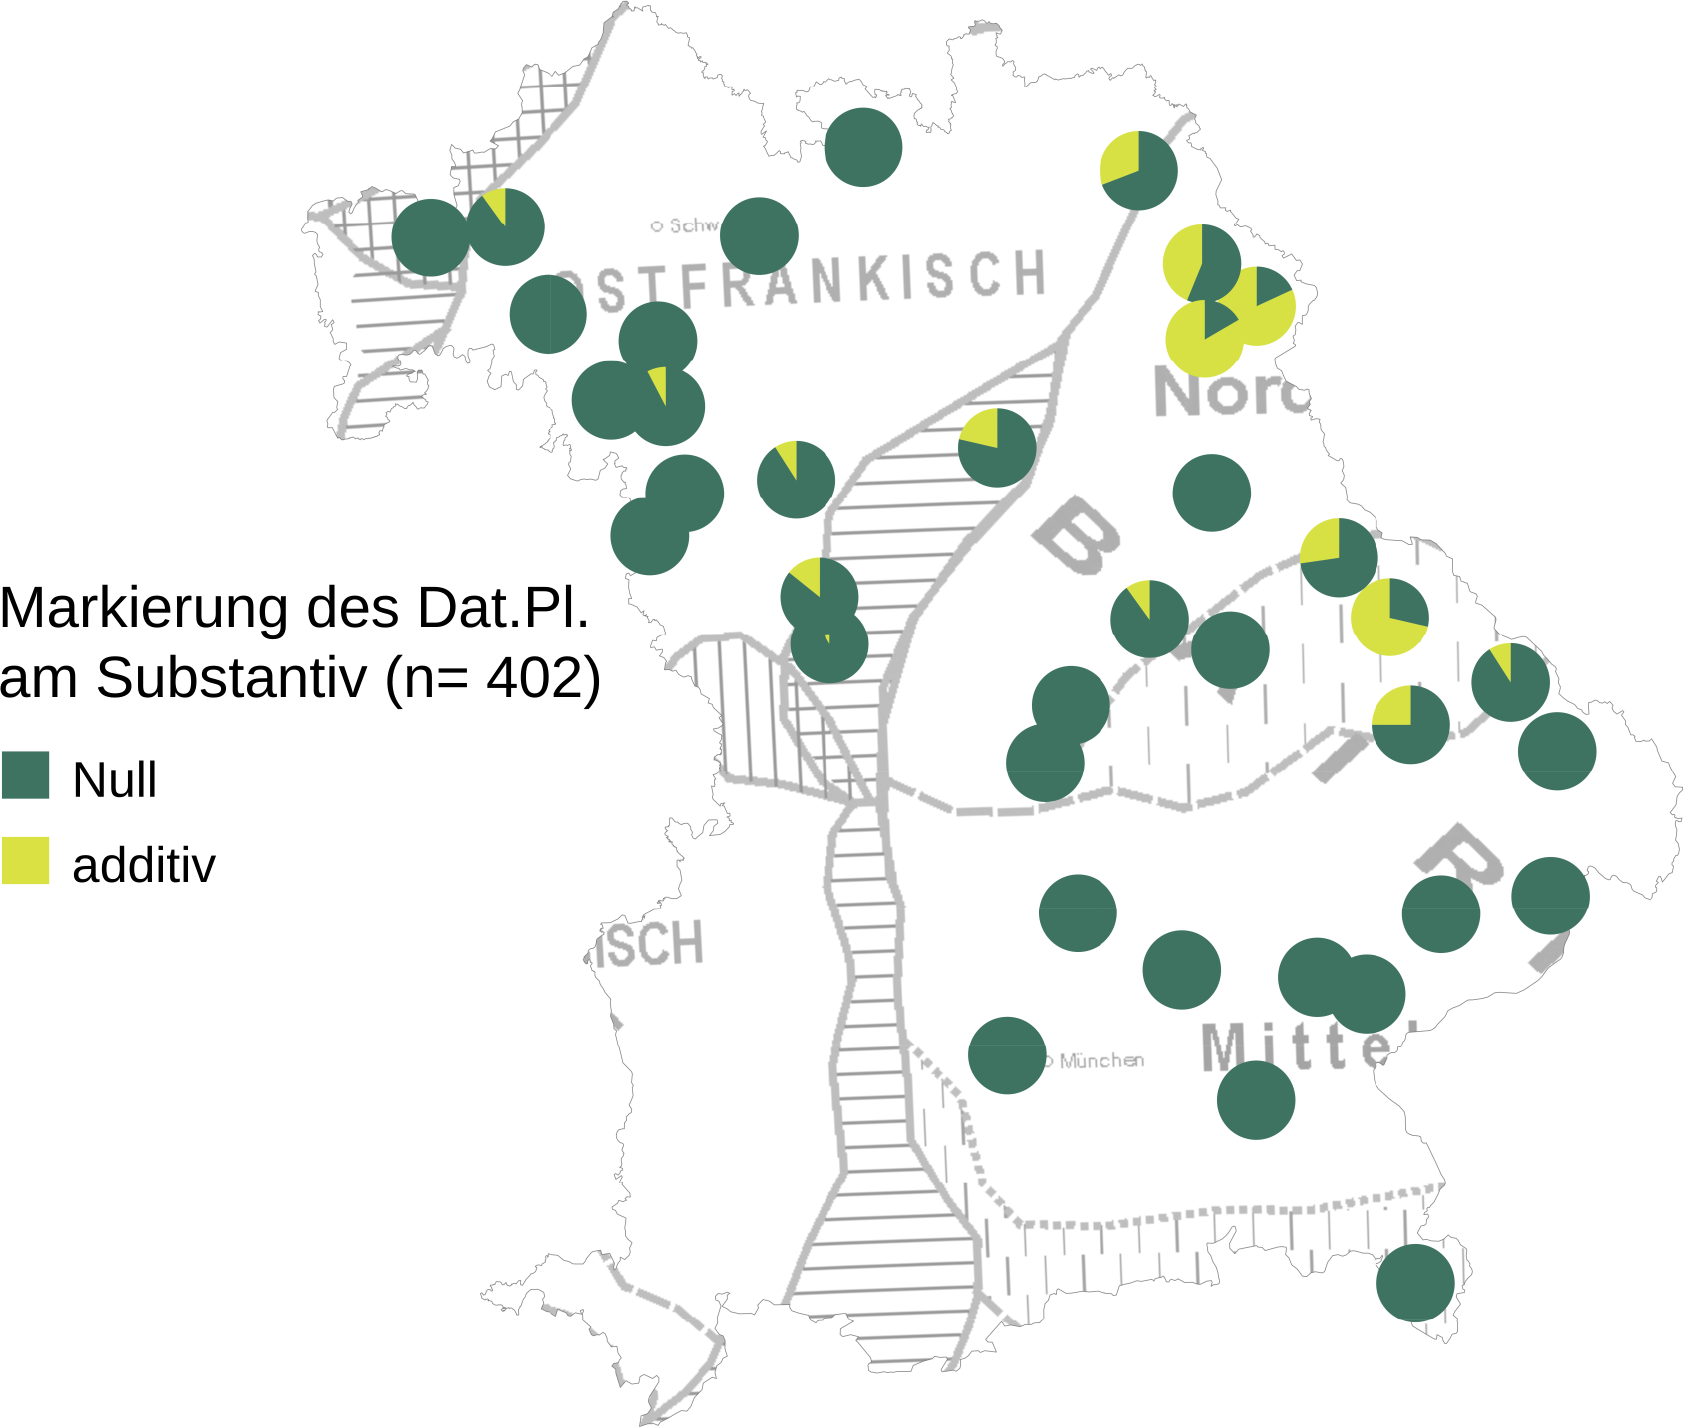
\includegraphics[width=.75\textwidth]{figures/Karte24.png}
\caption{Distinkte und synkretische Formen des Dat.Pl.}
\label{map:24}
\end{map}
\vfill\pagebreak

Im östlichen Ofr. (Tiefenbohrungspunkt Hallerstein) markiert das Suffix -\textit{na} den Dat.Pl. (bei Nasal im Auslaut des Nom.Pl. erscheint -\textit{α}, vgl. \citealt[139]{Rowley1997}): Nom.Pl. \teuthoo{k\_i“}{kʰī} -- Dat.Pl. \teuthoo{na}{na} \teuthoo{k\_ina}{kʰina} ‚Kühe‘, Nom.Pl. \teuthoo{ma942dla94}{ma\klammeruntenpost{}̣̄dla\klammeruntenpost{}̣} -- Dat.Pl. \teuthoo{den}{den} \teuthoo{glan}{ɡlan} \teuthoo{ma2dlana}{mādlana} ‚Mädchen‘, Nom.Pl. \teuthoo{di}{di} \teuthoo{k\_inEr}{kʰinər} -- Dat.Pl. \teuthoo{wel.An}{welͅαn} \teuthoo{k\_inana}{kʰinana} \teuthoo{ho.s}{hoͅs} \teuthoo{dus}{dus} \teuthoo{ge42m}{ɡẹ̄m} ‚welchen Kindern hast du es gegeben‘.\footnote{\citet[139]{Rowley1997} ebenso wie \citet[177]{Hermann1957} führen die Dativ-Plural-Form mit \textit{na}{}-Suffix auch für den Coburger Dialekt an, im Tiefenbohrungspunkt Ahorn finden sich indes nur synkretische Formen. Daneben gibt es Belege für Dativ-Plural-Formen mit \textit{na}{}-Suffix in historischen Dialektgrammatiken für das Ofr. Nürnbergs und Bambergs sowie das nördliche Nordbair. in Selb \textrm{(vgl. \citealt[§11]{Frommann1857}, \citealt[322--323]{Franke1895}, \citealt[262]{Schübel1955}, \citealt[32]{Vogt1930}).}} Von diesem dialektspezifischen Markierungstyp unterscheiden sich die nordbair. Dialekte systematisch, da hier einerseits die Form des Dativ-Plural-Markers variiert (distinkte Dativ-Plural-Formen enden auf Nasal, vgl. \citealt[139]{Rowley1997}) und es variiert -- zumindest im südlichen Nordbair. -- die präferierte Silbenstruktur: Auf die Stammsilbe können niemals zwei Reduktionssilben (Typ \teuthoo{ma2dlana}{mādlana}) folgen, sodass nach Nominativ-Plural-Formen mit den Reduktionssilben -\textit{α} und -\textit{el} ausschließlich das unsilbische Suffix \textit{{}-n} erscheint (\citealt[§147.2a]{Kollmer1987}, \citealt[140]{Rowley1997}).\footnote{Grundsätzlich ist es mit Blick auf die geringen Belegzahlen von distinkten Dativ-Plural-Formen pro Ortsdialekt schwierig, Aussagen über die Arealität der Verteilung zu treffen, es handelt sich allenfalls um Tendenzen. Erschwerend kommt hinzu, dass im bair. Teil, d.\,h. in den Teilprojekten SOB und SNiB weniger Dativ-Plural-Items abgefragt wurden als in den übrigen Projekten.} Dass diese Präferenz der Silbenstruktur auch innerhalb des Nordbair. variiert, zeigen \citegen[141]{Rowley1997} Belege aus dem nördlichen Nordbair.: Dat.Pl. \teuthoo{a4kanan}{ạkanan} ‚Äckern‘ (nordbair. Tirschenreuth), Dat.Pl. \teuthoo{autonan}{autonan} ‚Autos‘ (nordbair. Arzberg).\largerpage[2]

Ein weiterer systematischer Unterschied besteht innerhalb des Nordbair. hinsichtlich synkretischer vs. distinkter Dativ-Plural-Formen nach Reduktionssilbe -\textit{en}. Im mittleren und südlichen Nordbair. bilden Nominativ-Plural-Formen auf -\textit{en} keine distinkte Dativ-Plural-Form (z.\,B. im nordbair.-mittelbair. Blaibach Nom.Pl. \teuthoo{unsAne4}{unsαnẹ} \teuthoo{k\_a9.tSn@}{kʰa\klammeruntenpost{}ͅtʃn̥} -- Dat.Pl. \teuthoo{mid}{mid} \teuthoo{unsene4}{unsenẹ} \teuthoo{kha).tSn@}{kha\klammeruntenpost{}ͅtʃn̥} ‚mit unseren Katzen‘, vgl. \citealt[87]{Bachmann2000}, \citealt[§147.2b]{Kollmer1987}, \citealt[140]{Rowley1997}). Im nördlichen Nordbair. ersetzt das Dativ-Plural-Suffix {}-\textit{αn} das Nasalsuffix -\textit{n} der Nominativ-Plural-Form bei mhd. schwachen Feminina und Maskulina sowie bei zweisilbigen Maskulina mit Reduktionssilbe -\textit{en}: Nom.Pl. \teuthoo{unE}{unə} \teuthoo{g\_åtSn@}{ɡʰ{\burgeroalpha}tʃn̥} -- Dat.Pl. \teuthoo{mid}{mid} \teuthoo{unEn}{unən} \teuthoo{g\_åtSAn@}{ɡʰ{\burgeroalpha}tʃαn̥} ‚Katzen‘ (Groschlattengrün), Nom.Pl. \teuthoo{khi“En}{khīən} -- Dat.Pl. \teuthoo{midn@}{midn̥} \teuthoo{k\_ôe.ikhi“EdAn}{kʰ{\aufstrih}eͅikhīədαn} ‚mit den Kuhketten‘ (Tirschenreuth), Nom.Pl. \teuthoo{bôo<u.m}{b{\aufstrih}ôuͅm} -- Dat.Pl. \teuthoo{min}{min} \teuthoo{b5ôo>?(?u.BAn}{b̩{\aufstrih}ö̂̈\klammerobenpost{}uͅ{\btilde}αn} ‚mit den Buben‘ (Windischeschenbach, vgl. \citealt[20]{Micko1933}, \citealt[142]{Rowley1997}, \citealt[§574]{Schmeller1821}). \citet[174]{Schnabel2000} führt diese Form der Suffixalternation auch für das ofr. Weingarts an, wenngleich diese Form der Formenbildung „zurückgedrängt“ werde, z.\,B. Nom./
Akk.Pl. \teuthoo{xo2sn}{xōsn} -- Dat.Pl. \teuthoo{xo2se.n}{xōseͅn} ‚Hase‘. Wie auch im Bereich der additiven Pluralmarkierung stellt die Suffixalternation hier einen Grenzfall des additiven Verfahrens dar (ausführlicher hierzu \sectref{sec:7.1.1.4}).

Im nördlichen Nordbair. (Tiefenbohrungspunkte Groschlattengrün, Tirschenreuth, Windischeschenbach) weisen distinkte Dativ-Plural-Formen eine (mindestens) zweisilbige Outputstruktur mit Reduktionssilbe -\textit{αn} auf, die durch die Addition unsilbischer und silbischer Kasussuffixe bzw. durch Suffixalternation gebildet wird:

\begin{itemize}
\item {}-\textbf{\textit{n}} nach der Reduktionssilbe -\textit{α} im Nom.Pl.: Nom.Pl. \teuthoo{mo<i.d49ýA}{môiͅḍ\klammeruntenpost{}ɫα} -- Dat.Pl. \teuthoo{deAn}{deαn} \teuthoo{glo+i.6n}{ɡlõĩͅn} \teuthoo{mo<8i.d49lAn}{mô\klammerobenpost{}iͅḍ\klammeruntenpost{}lαn} \teuthoo{ge4<m}{ɡệm} ‚den kleinen Mädchen gegeben‘ (nordbair. Windischeschenbach), Nom.Pl. \teuthoo{ta4rmA}{tạrmα} -- Dat.Pl. \teuthoo{i.}{iͅ} \teuthoo{t,a4rmAn}{t͓ạrmαn} ‚in den Därmen‘ (nordbair. Tirschenreuth)
\item {}-\textbf{\textit{αn}} bei einsilbigen Pluralformen oder nach Reduktionssilbe -\textit{el}: Nom.Pl. \teuthoo{the94nt\_}{the\klammeruntenpost{}̣ntʰ} -- Dat.Pl. \teuthoo{ån}{{\burgeroalpha}n} \teuthoo{hentAn}{hentαn} ‚an den Händen‘ (nordbair. Windischeschenbach), Nom.Pl. \teuthoo{gð\_E<i.}{ɡ̩ʰə̂iͅ} -- Dat.Pl. \teuthoo{unEn}{unən} \teuthoo{g\_E<i.En}{ɡʰə̂iͅən} ‚unseren Kühen‘ (nordbair. Windischeschenbach), Nom.Pl. \teuthoo{vi“Egl@}{vīəɡl̥} -- Dat.Pl. \teuthoo{vi“EglAn}{vīəɡlαn} ‚Vögel‘ (nordbair. Tirschenreuth, vgl. \citealt[142]{Rowley1997})
\item Suffixalternation \textbf{{}-}\textbf{\textit{n}} > \textbf{-\textit{αn}} nach Reduktionssilbe -\textit{en} im Nom.Pl.
\end{itemize}

Neben dieser präferierten Outputstruktur des nördlichen Nordbair. kann die Distribution der Dativ-Plural-Allomorphe durch den Auslaut der No\-mi\-na\-tiv-""Plu\-ral-""Form bedingt sein. So erscheint nach \citet[87]{Bachmann2000} im nordbair. Eslarn beispielsweise das Allomorph {}-\textit{nαn} nach Dentalplosiv (vgl. Nom.Sg./Nom.Pl. \teuthoo{he.nt\_}{heͅntʰ} -- Dat.Pl. \teuthoo{i.}{iͅ} \teuthoo{he.ndnAn}{heͅndnαn} ‚an den Händen‘ im nord\-bair.-""mit\-tel\-bair. Blaibach).\footnote{Vgl. hierzu \citealt{WA}-Karte 543 „Leuten“: Im nordbair. Kallmünz ist die Dativ-Plural-Form als \textit{mit’n Leunan} übersetzt. Der Dentalplosiv des Stammauslauts ist hier an das Kasusflexiv -\textit{nαn} assimiliert, was laut \citet[143]{Rowley1997} nach besonders frequenten Lexemen wie \textit{Leute} und \textit{Tag} auftritt.} Das Allomorph -\textit{αn} erscheint nach \citet[141]{Rowley1997} im mittleren und südlichen Nordbair. regelmäßig nach nasaliertem Vokal oder Diphthong: Nom.Pl. \teuthoo{k,\_ôe2i“}{k͓ʰ{\aufstrih}ēī} -- Dat.Pl. \teuthoo{An}{αn} \teuthoo{k\_ôeiAn}{kʰ{\aufstrih}eiαn} ‚Kühe‘ im nordbair. Kallmünz (vgl. \citealt[§147]{Kollmer1987}). Die Zusammenschau der eigenen Daten und der Darstellungen in Dialektgrammatiken zeigt indes, dass die Distribution der Allomorphe zumindest teilweise lexikalisch bedingt oder frei zu sein scheint \citep[142]{Rowley1997}.

Dass im Bair. die Allomorphe -\textit{αn}, -\textit{nan} und (mit elidiertem auslautendem Nasal) -\textit{na} im Ofr., teilweise auch im nördlichen Nordbair. für den Dat.Pl. zur Verfügung stehen, ist das Ergebnis eines dialektraumspezifischen diachronen Prozesses. Für das Mittelhochdeutsche modellieren \citet[125]{KleinEtAl2018} die Regel, dass Dat.Pl. in der Regel mit -\textit{(e)n} markiert wird, nur nach mhd. -\textit{en} in der Reduktionssilbe des Singularstammes (Typ mhd. \textit{wagen}) oder als Pluralmarker erscheint das Kasusflexiv nicht (trotz gelegentlicher Belege, vgl. \citealt[127--128]{KleinEtAl2018}). Diese Restriktion ist, wie oben dargestellt, im UG teilweise aufgehoben, die Ausdehnung der Dativ-Plural-Markierung nach Reduktionssilbe -\textit{en} führt diachron zur Herausbildung dialektspezifischer Marker der Kasusinformation, die schließlich auf alle Genera und Umgebungen ausgedehnt werden (\citealt[§285]{Gebhardt1907}, \citealt[§56]{Kollmer1985}, \citealt[§810]{Schmeller1821}). \citet[441--442]{Schirmunski1962} bezeichnet die Suffigierung mit dem Suffix -\textit{αn} als „‚potenzierte‘ Endung“ (< \textit{en-en}), für die er Belege aus dem Nordbair., dem ostmittelbair. Neuenkirchen und daneben auch im Ostmitteldeutschen anführt (vgl. \citealt[§863]{Schmeller1821}, der den „ostlechischen Dialekt“ als Verbreitungsgebiet angibt). Diese Form der Dativ-Plural-Markierung erscheint damit in jenen Dialekten, die die Tendenz einer synkretischen Form der Kasusmarkierung von Dativ und Akkusativ zugunsten des Akkusativs aufweisen, das potenzierte Dativ-Plural-Suffix markiert eine „Tendenz zur Festigung der morphologisch differenzierten Kasusform“ (\citealt[442]{Schirmunski1962}, vgl. \sectref{sec:7.2.2} sowie \citealt[§145]{Kollmer1987}, \citealt[§20]{Micko-Repp1933}, \citealt[327--328]{Schiepek1908}). Die jüngeren Daten der BSA-Erhebungen (und hierin auch die Gewährspersonenkommentare) zeigen indes, dass sich das Dialektmerkmal eines erweiterten Nasalsuffixes {}-\textit{nen} zumindest im UG des SMF im Abbau befindet (\citealt[120]{SMF7}).

\subsection{Kasusmarkierung und Kasussynkretismen}\label{sec:7.2.2}\largerpage
\begin{sloppypar}
Die Inventarisierung der Kasusmarkierungsstrategien und -marker in \sectref{sec:7.2.1} hat gezeigt, dass im Bereich der dialektalen Kasusmarkierung zwei zentrale Befunde zu konstatieren sind: Diachron findet ein Abbau der Kasusmarkierung am Substantiv statt, innerparadigmatische Synkretismen nehmen zu. Gleichzeitig gibt es dialektspezifische Marker (im Dat.Pl.) sowie dialektspezifische, morphophonologisch bedingte Muster (Nom.Sg. \teuthoo{k,\_a.rpfA}{k͓ʰaͅrpfα} -- Akk.Sg. \teuthoo{An}{αn} \teuthoo{k,\_a.rpfAn}{k͓ʰaͅrpfαn} im Nordbair.). In \sectref{sec:7.1.3.1} wurde bereits im Fall rezenter Nullplurale gezeigt, dass die Neutralisierung distinkter Formen ein kontrastives Phänomen darstellt: Synchrone Synkretismen ergeben sich im diachronen Vergleich oder aus dem Vergleich synchroner Diasysteme (vgl. \citealt[1170]{Panzer1983}). Synchrone Synkretismen sind auch mit Blick auf die areale Dimension von Morphologie interessant, da sich Dialektsysteme dieselben Flexionskategorien teilen, aber die Konstellationen von distinkten und synkretischen Formen im Paradigma variieren: „paradigmatic distinctions contribute notably to the constitution of linguistic areas“ \citep[808]{Rabanus2010}. Im Bereich der Kasusmorphologie gilt (auch mit Blick auf die Entwicklung des Neuhochdeutschen), dass Kasusmarkierung zwar am Substantiv, nicht aber gänzlich abgebaut wird; die Markierung geht von der morphologischen in die morphosyntaktische Domäne über.
\end{sloppypar}

Das synchrone Kasussystem der untersuchten Dialekte ist auf drei Kasus reduziert: Nominativ, Akkusativ, Dativ. Hinsichtlich der syntaktischen Funktion werden Subjekt, direktes und indirektes Objekt unterschieden. Der Genitiv erscheint „völlig isoliert“ \citep[90]{Rowley1997} und ist nur noch in wenigen festen Wendungen erhalten, weshalb er im Folgenden nicht behandelt wird. Für die verbleibenden Kasus können für die drei Genera synchron die in  \figref{fig:8} dargestellten Paradigmenkonstellationen im Singular und Plural beschrieben werden. Die Auswertung der Kasusformen zeigt, dass für das Paradigma der Maskulina und -- zumindest im Bair. -- bei den Feminina im Singular und für das Pluralparadigma jeweils zwei Varianten angesetzt werden können: (1) weist jeweils völligen Kasussynkretismus auf, in (2) sind distinkte Formen in den obliquen Kasus der Maskulina bzw. im Dativ bewahrt. Bei den Neutra sind markierte Formen in den untersuchten Dialekten nur vereinzelt im Dat.Sg. belegt (durch die Schraffierung symbolisiert). Laut \citet[88]{Rowley1997} konnte die distinkte Dativ-Singular-Form des Neutrums \textit{Herz} nur in der idiomatisierten Wendung „von Herzen“ elizitiert werden, in den eigenen Daten ist sie als Einzelbeleg mit Nasalflexiv nur im nordbair.-mittelbair. Grafenkirchen belegt, die übrigen Dativ-Singular-Formen von \textit{Herz} weisen Nullmarkierung auf: Nom.Sg. \teuthoo{he.EtS}{heͅətʃ} -- Dat.Sg. \teuthoo{a.m}{aͅm} \teuthoo{he.EtSn@}{heͅətʃn̥} -- Nom.Pl. \teuthoo{he.EtSn@}{heͅətʃn̥} (vgl. \citealt{WA}-Karte 477 „Herzen“).


\begin{figure}%abb.7.6
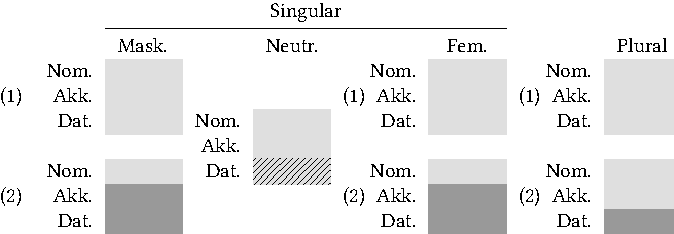
\includegraphics[width=\textwidth]{figures/fig7-6.pdf}
\caption{Paradigmenkonstellation der Substantivflexion im Singular und Plural (vgl. \citealt[88]{Rowley1997})}
\label{fig:8}
\end{figure}

Das distinkte Singular-Kasusparadigma (2) der Feminina umfasst nur eine kleine Klasse: die Verwandtschaftsbezeichnungen \textit{Mutter} und \textit{Schwester}. Nach \citet[137]{Rowley1997} flektieren auch \textit{Tochter} und \textit{Schwieger} ‚Schwiegermutter‘ sowie die mask. Verwandtschaftsbezeichnungen \textit{Bruder}, \textit{Gevatter}, \textit{Schwager}, \textit{Vater}, \textit{Vetter} nach dem Muster der schwachen Deklination, sodass im südlichen Nordbair. und im Mittelbair. eine semantisch konditionierte Deklinationsklasse ‚enge Verwandtschaftsbezeichnungen‘ anzusetzen ist (vgl. \citealt[122]{Steininger1994} und \sectref{sec:8.3.2.2}.). \mapref{map:25} zeigt, dass sich diese Paradigmenkonstellation nur im nord\-bair.-""mit\-tel\-bair. Übergangsgebiet und vereinzelt im Mittelbair. findet, die Paradigmenkonstellation (1) mit synkretischem Singularparadigma und Plural mit Nasalsuffix ist im Nordbair. und in Teilen des Ofr. belegt.{\interfootnotelinepenalty=10000\footnote{In den BSA-Erhebungen wurde für \textit{Mutter} nur die Dativ-Singular-Form abgefragt. Nach \citet[137]{Rowley1997} stellen die schwach flektierenden Feminina insofern eine Besonderheit dar, als die Akkusativ-Singular-Form (als bei den schwachen Maskulina) keine Markierung aufweist. Der vermutete Synkretismus in den eigenen Tiefenbohrungspunkten wird durch Schraffur dargestellt.}}
Daneben ist vereinzelt im Mittelbair. eine Art Mischparadigma mit Nasalflexiv im Dat.Sg. und Umlautplural belegt.\footnote{Ein solches Mischparadigma führt \citet[88]{Eich1925} auch für das Maskulinum \textit{Tropf} „‚nichtswürdiger Kerl‘“ an: schwache Deklination (d.\,h. vokalisch realisiertem Nasalsuffix) im Singular, Umlautmarkierung im Plural (Dat.Sg. \teuthoo{mI5de.An}{mideͅαn} \teuthoo{dro3bfe}{drŏbfe}, Pl. \teuthoo{dre3bf}{drĕbf}).}

\begin{map}
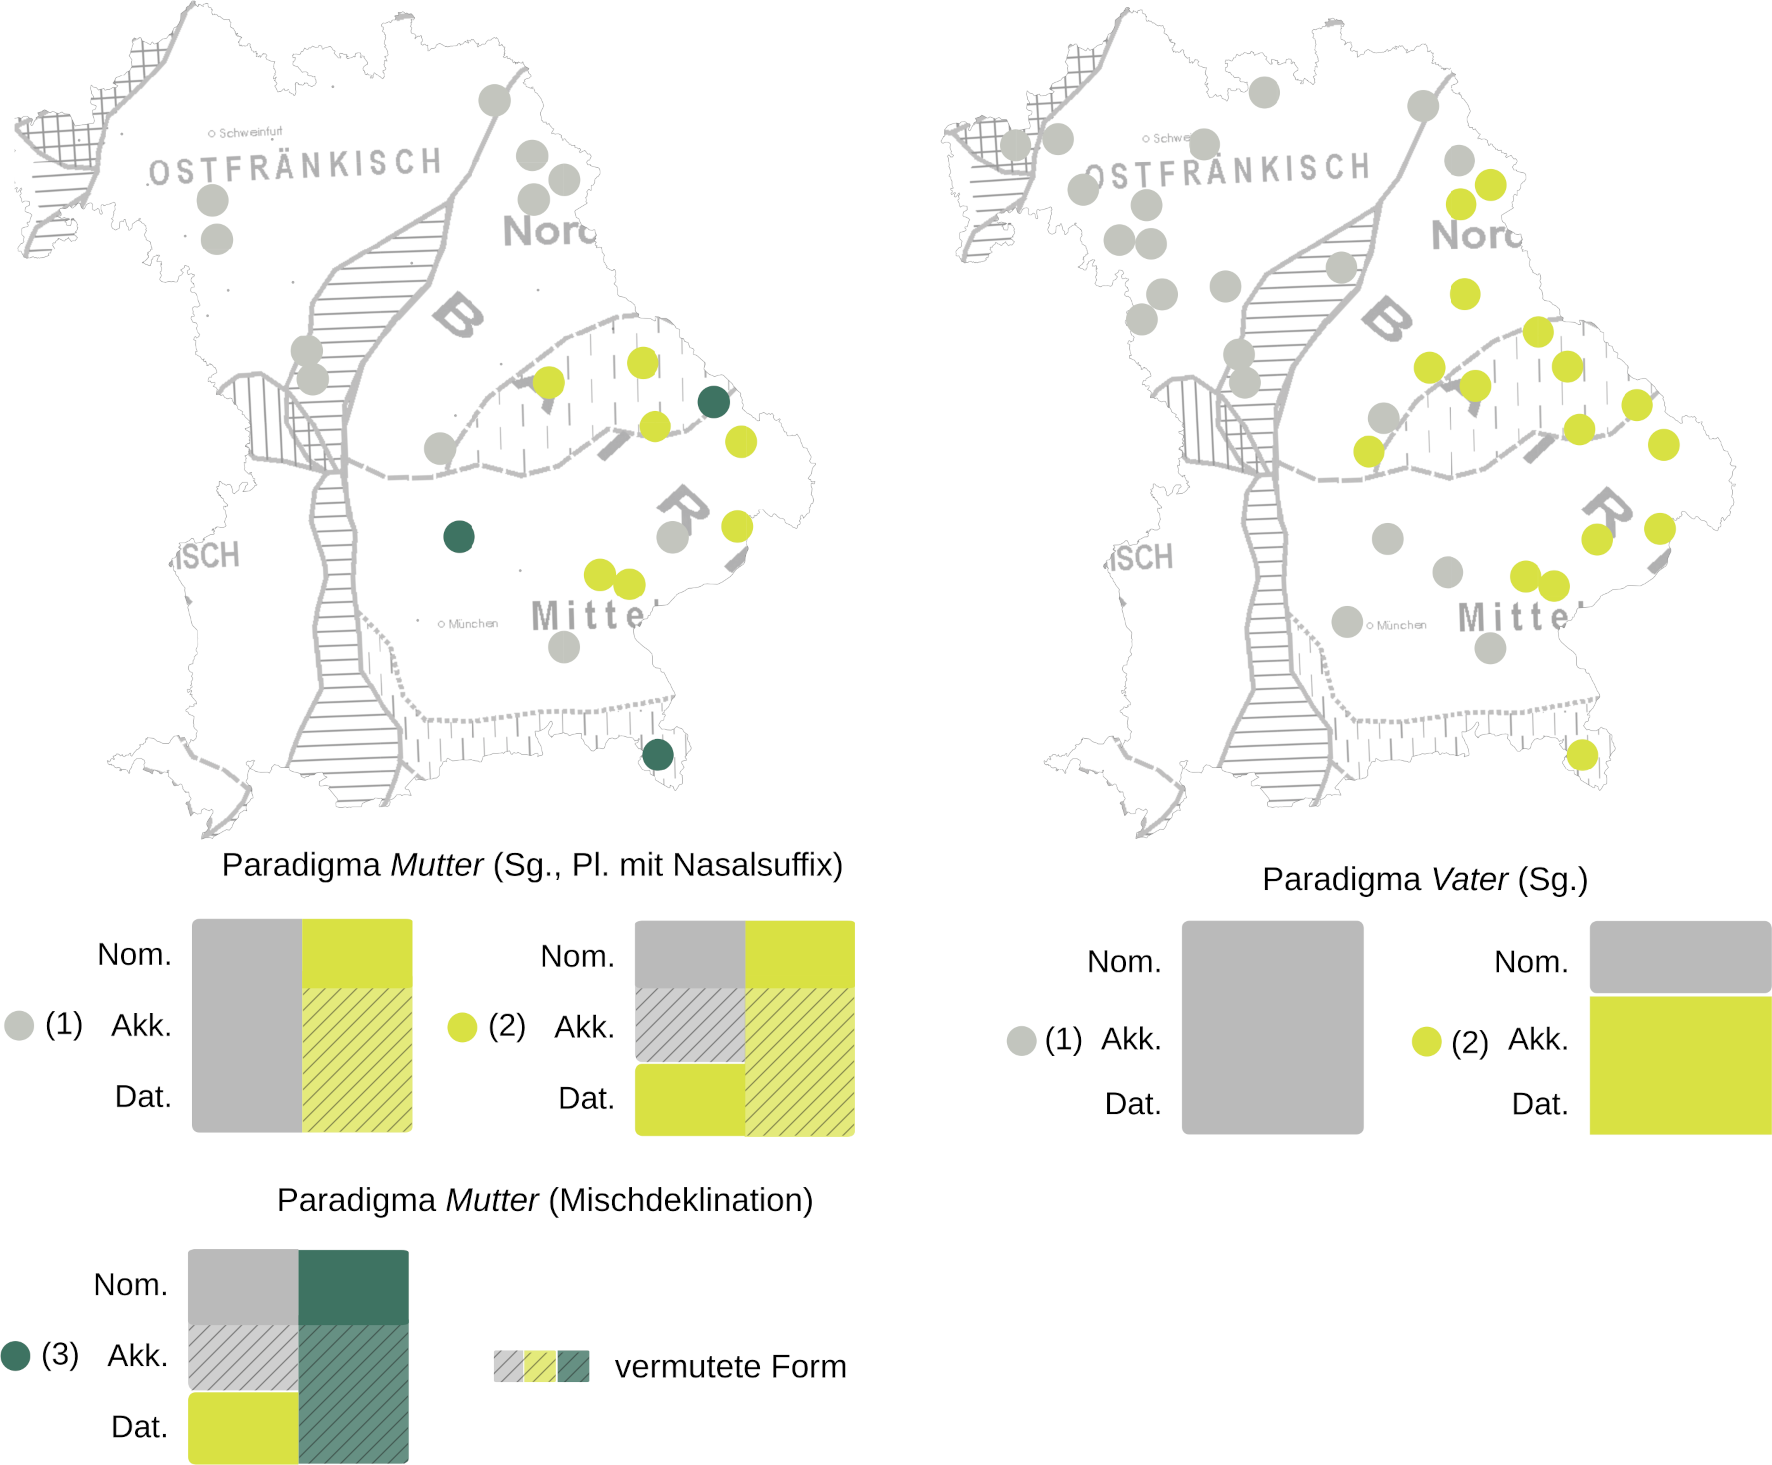
\includegraphics[width=\textwidth]{figures/Karte25.png}
\caption{Areale Verteilung der Paradigmen der schwachen Verwandtschaftsbezeichnungen \textit{Mutter} und \textit{Vater}}
\label{map:25}
\end{map}


Das Maskulinum \textit{Vater} gehört ebenfalls zu der semantisch konditionierten Deklinationsklasse „Verwandtschaftsbezeichnungen“. Die Verbreitung der distinkten Akkusativ- und Dativ-Singular-Formen ist hier noch größer als bei \textit{Mutter} (Pluralformen wurden in den BSA-Erhebungen nicht abgefragt). Bemerkenswert sind die Fälle von intraindividueller Variation, die sich (zumindest vor der Folie der schriftsprachlichen Kasusrelationen) für die in verschiedenen Kontexten abgefragten obliquen Kasusformen von \textit{Vater} und auch in der Form der Artikel in den bair. Ortsdialekten ergeben, z.\,B. exemplarisch im nordbair. Windischeschenbach \teuthoo{dEi.}{dəiͅ} \teuthoo{ho)4m}{ho\klammeruntenpost{}̣m} \teuthoo{unEm}{unəm} \teuthoo{våtEn}{v{\burgeroalpha}tən} \teuthoo{g\_ul.d5}{ɡʰulͅd̩} ‚sie haben unseren Vater vom Feld geholt‘, \teuthoo{dEi.}{dəiͅ} \teuthoo{hôo2.o4d}{h{\aufstrih}ōͅọd} \teuthoo{qi>ErEm}{ʔîərəm} \teuthoo{våtA}{v{\burgeroalpha}tα} \teuthoo{qå"glu.<EN}{ʔ{\burgeroalphamakron}ɡlûͅəŋ} ‚sie hat ihren Vater angelogen‘, \teuthoo{i“BA}{ī{\btilde}α} \teuthoo{qi>ErEn}{ʔîərən} \teuthoo{våtAn}{v{\burgeroalpha}tαn} \teuthoo{gs\#imb5f,d}{ɡšimb̩f͓d} ‚über ihren Vater geschimpft‘.

Neben den schwachen Flexionsformen dieser kleinen Klasse von Substantiven finden sich Paradigmenkonstellationen dieses Typs bei den mhd. schwachen Maskulina. Eine Schwierigkeit bei der Auswertung der schwachen Maskulina besteht in der Datenlage. Nicht alle Lexeme wurden in allen Teilprojekten in der Akkusativ-Singular-Form abgefragt, für die SNiB- und SOB-""Tie"-fen"-boh"-rungs"-punk"-te sind nur ein bis zwei Formen belegt, sodass die Datenauswertung für dieses Gebiet unbefriedigend bleibt.


\begin{map}
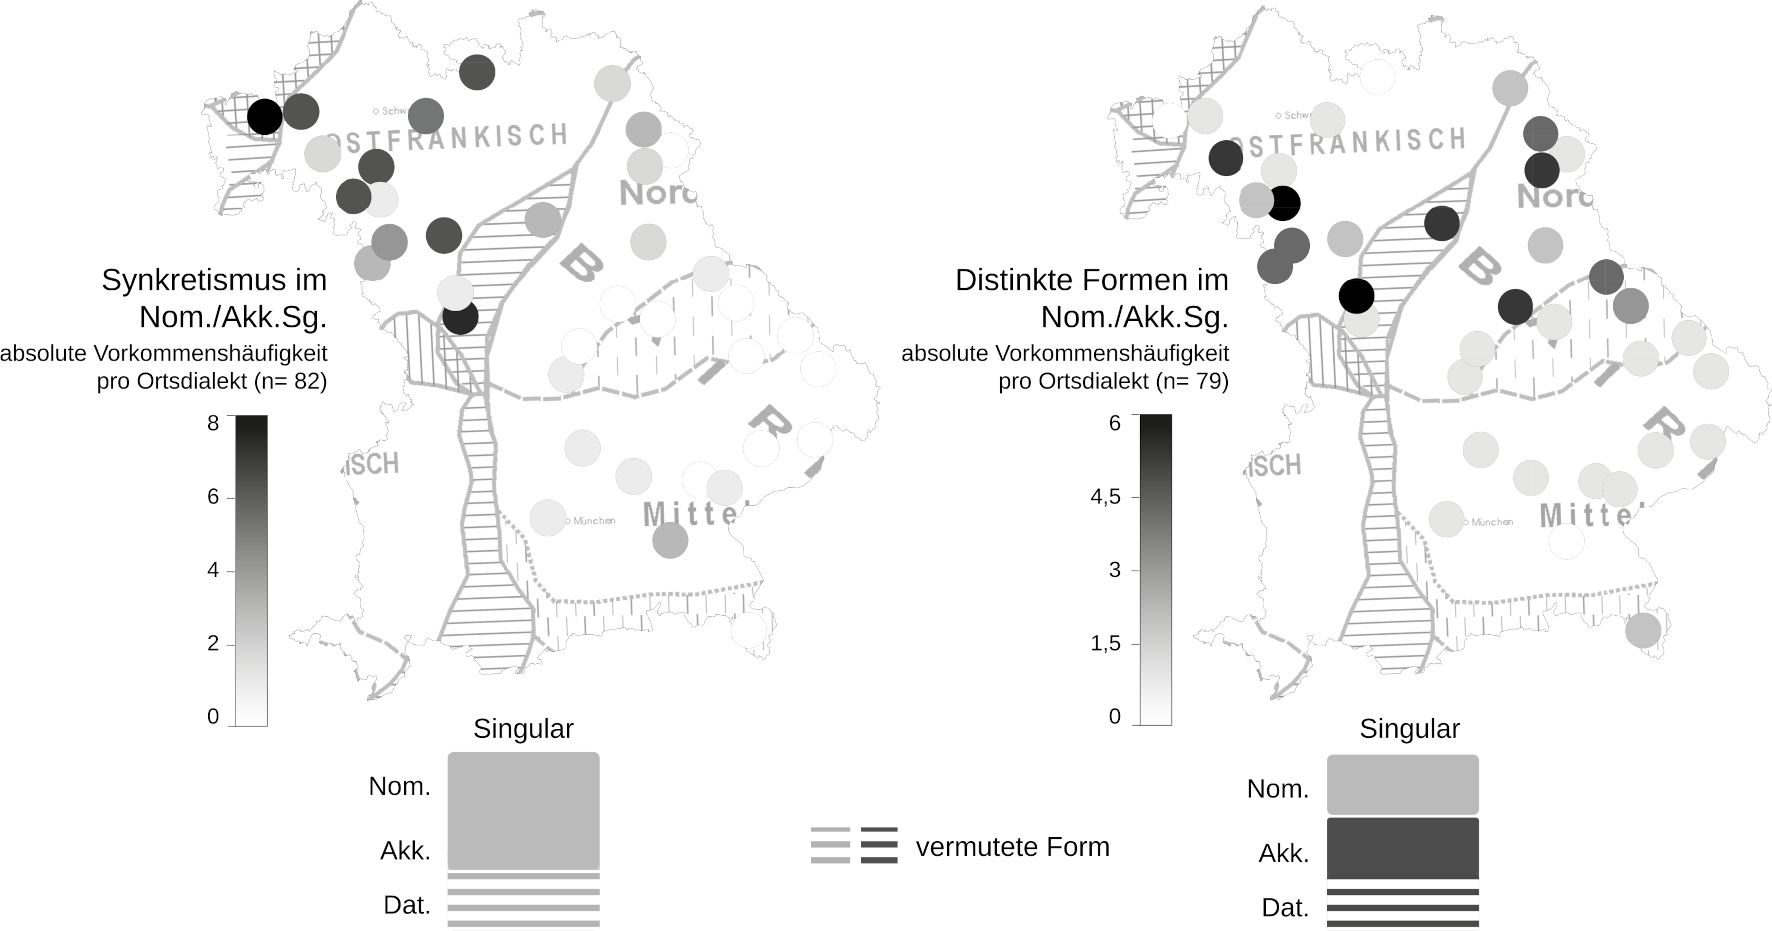
\includegraphics[width=\textwidth]{figures/Karte26.png}
\caption{Synkretismen und Distinktionen Singularparadigma der schwachen Maskulina (\teuthoo{n=}{ǹ} 161)}
\label{map:26}
\end{map}

\mapref{map:26} visualisiert in Form von Chloroplethkarten die Verteilung der beiden möglichen Paradigmenkonstellationen in absoluten Zahlen (Synkretismus durch Nullmarkierung im Akk.Sg. und Dat.Sg. vs. Distinktion durch additive Markierung).\footnote{Die Dativ-Singular-Form wurde in den BSA-Erhebungen leider nicht abgefragt, siehe aber beispielsweise \citet[§20]{Micko-Repp1933} oder \citet[§7]{Schübel1955} zu vollständigen Paradigmen.}  Im Ofr. gibt es die Tendenz zu Synkretismen. Im ofr. Ahorn und im ofr. Wiesthal gibt es keine Belege für distinkte Singularparadigmen; die Markierung der obliquen Singularkasus ist hier abgebaut. In den nordbair. Tiefenbohrungspunkten mit guter Datenlage gibt es eine eindeutige Tendenz zu distinkten Paradigmen, während es im westlichen Streifen des Ofr. ein Nebeneinander synkretischer und distinkter Formen gibt, das durch die semantische Distinktion [+belebt] und [${\pm}$menschlich] konditioniert ist (hierzu ausführlicher \sectref{sec:8.3.2.2}).

Auch \citet[183]{HarnischRowley1990} zeigen, dass die areale Verteilung distinkter obliquer Formen in der schwachen Deklination durch die semantischen Merkmale [+belebt] und [+menschlich] gesteuert ist. In einem südlichen oberofr. Gebiet (um Bamberg, Kronach) erscheint eine distinkte Markierung bei belebten Maskulina (\textit{Bube}, \textit{Hase}), im nordöstlichen oberofr. Gebiet um Coburg (Tiefenbohrungspunkt Ahorn) erscheinen synkretischen Formen. In einer Übergangszone (um Marktgraitz, Lichtenfels) zwischen diesen beiden Gebieten mit distinkter vs. synkretischer Form werden nur belebte, menschliche Denotate schwach flektiert (d.\,h. \textit{Bube}, nicht aber \textit{Hase}, vgl. \citealt[155 und 191]{Rowley1997}). Das Mosaik-Plot in  \figref{fig:9} visualisiert die Variablen Lexem, Form der Markierung im Akk.Sg. und absolute Häufigkeit. Die Größe der Flächen der Rechtecke ist dabei relativ zur Häufigkeit der Lexeme in den Daten zu lesen. Damit bestätigt das Plot -- ohne Berücksichtigung der arealen Dimension -- den Befund, dass Maskulina mit der Semantik [+belebt] und [+menschlich] eher distinkte Akkusativ-Singular-Formen aufweisen, aber auch, dass synkretische vs. distinkte Paradigmen darüber hinaus lexikalisch oder durch Frequenzeffekte bedingt zu sein scheinen (vgl. \mapref{map:30} für die areale Dimension).\footnote{Daneben werden „Abweichungen“ vom „vorherrschenden Kasussynkretismus“ im SMF auf Unsicherheiten der Gewährspersonen zurückgeführt \citealt[19]{SMF7}).}


\begin{figure}
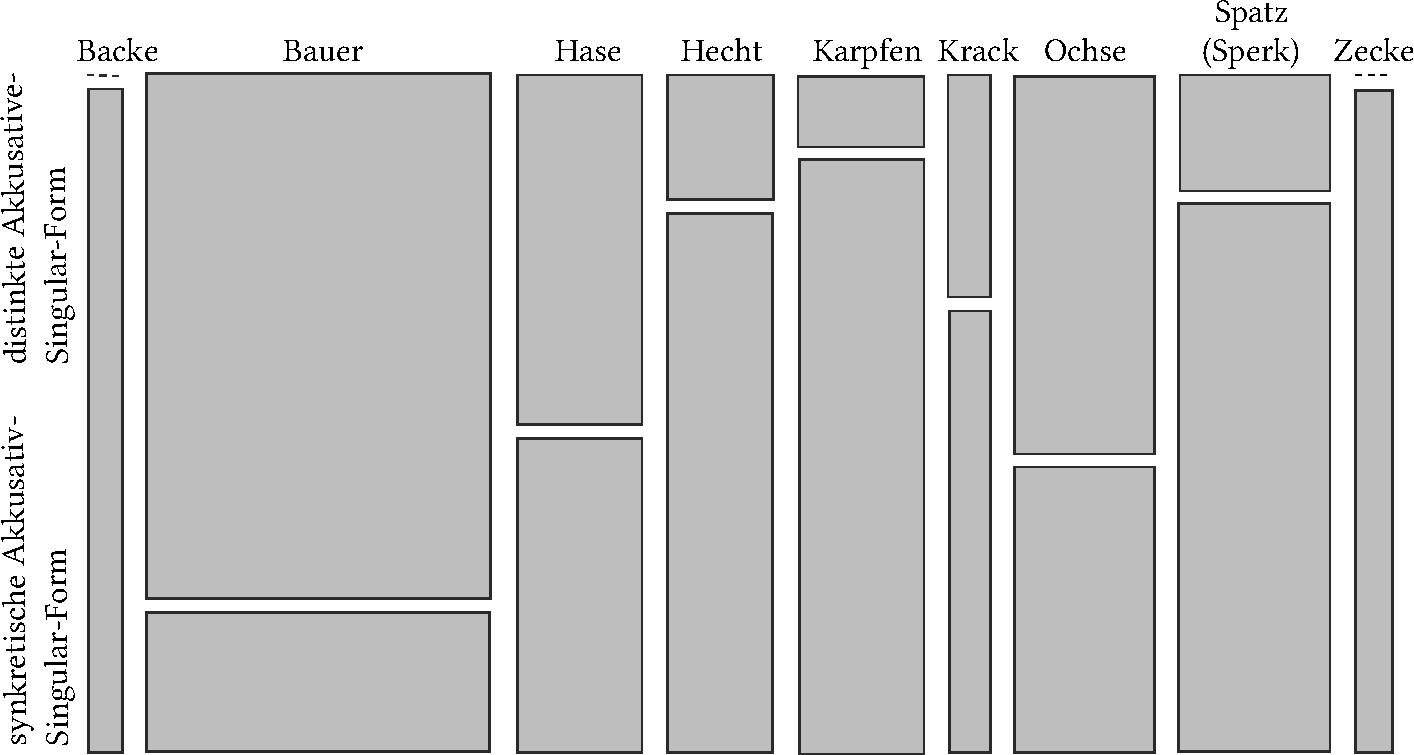
\includegraphics[width=\textwidth]{figures/revisedNickelNominalmorphologie-img038.pdf}
\caption{Mosaik-Plot mit Häufigkeitsverteilung der Akkusativ-Singular-Markierung der schwachen Maskulina ($n=164$)}
\label{fig:9}
\end{figure}

Daneben bedingt im Falle von \textit{Karpfen} die zweisilbige Struktur auf Reduktionssilbe mhd. -\textit{en} die Markierung im Ofr. und im Nordbair. und damit die Paradigmenzusammensetzung aus distinkten und synkretischen Formen (vgl. \sectref{sec:7.2.1}). Im Ofr. liegt Paradigmenkonstellation (1) mit völligem Synkretismus von Numerus und Kasus (Typ \textit{Karpfen} -- \textit{Karpfen}) vor, in Teilen des Nordbair. hingegen ergibt sich ein distinktes (dialektspezifisches) Paradigma (2) mit schwacher Markierung in den obliquen Kasus im Singular und im Plural (\figref{fig:10}). Vergleicht man diese Konstellation nun mit dem Paradigma von \textit{Eiche}, so ergeben sich ähnliche und wiederum dialektspezifische Konstellationen. \textit{Eiche} gehört im Mittelhochdeutschen zur starken Deklination, in den rezenten Dialekten des UGs flektiert es wie die nhd. Klasse der zweisilbigen Feminina mit Schwa-Reduktionssilbe (siehe \sectref{sec:7.1.3.1} zur Problematik des Bezugssystems). Im Ofr. findet sich völliger Synkretismus in Numerus und Kasus, in den bair. Ortsdialekten ist mehrheitlich Paradigma (2) mit einer distinkten Form im Plural belegt (Typ \teuthoo{oAxA}{oαxα} -- \teuthoo{oAxAn}{oαxαn}). Daneben finden sich im Bair. zwei distinkte Paradigmen: (3) im nordbair.-mittelbair. Grafenkirchen und (4) im mittelbair. Reischach. Damit sind distinkte Paradigmen bei den Feminina nicht nur bei Verwandtschaftsbezeichnungen anzunehmen, sondern auch bei nhd. zweisilbigen Feminina mit Schwa-Reduktionssilbe -- in welchem Umfang muss mit Blick auf die Datenlage leider offenbleiben.

\begin{figure}%7.8
\begin{tabular}{@{}p{0.5\textwidth}@{}p{0.5\textwidth}@{}}
  \vspace{0pt} 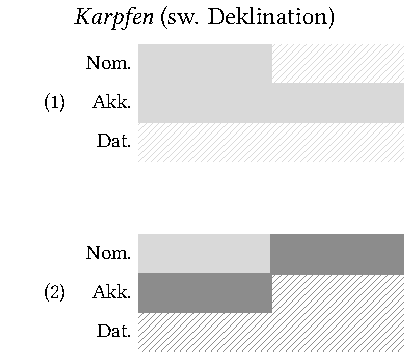
\includegraphics[width=0.49\textwidth]{figures/fig7-8-1.pdf} &
  \vspace{0pt} 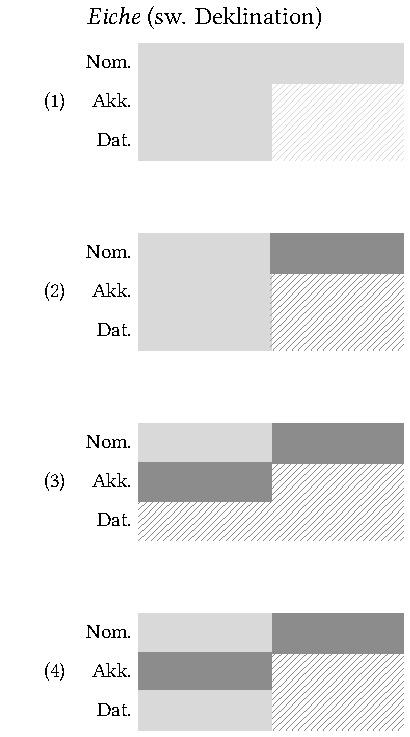
\includegraphics[width=0.49\textwidth]{figures/fig7-8-2.pdf}
\end{tabular}
\caption{Schwache Paradigmenkonstellation bei Reduktionssilbe mhd. -\textit{en}}
\label{fig:10}
\end{figure}

Laut \citet[91]{Rowley1997} werden Akkusativ und Dativ in ihren jeweiligen syntaktischen Funktionen als direktes bzw. indirektes Objekt in den Dialekten seines nordostbayrischen UGs differenziert, wenngleich sich eine Aufhebung der formalen (d.\,h. morphologischen) Distinktion beider Kasus andeute.\footnote{Auch für das unterofr. Aschenroth (Tiefenbohrungspunkt Gemünden am Main) gibt \citet[16]{Köhler1934} einen fast durchgehenden Zusammenfall von Dativ und Akkusativ an, bemerkt aber, dass der Dativ trotzdem „im Sprachgefühl noch vom Akkusativ unterschieden“ werde.}  Im Ofr. und im Regensburger Umland sei das Elizitieren additiver Dativ-Plural-Formen schwieriger als im nördlichen Nordbair. gewesen (d.\,h. in jenem Gebiet, für das \mapref{map:24} den höchsten Anteil distinkter Dativ-Plural-Formen ausweist), junge Dialektsprecher im ofr. Bayreuth und Coburg sowie im nordbair. Amberg und Regensburg hielten die additiven Formen für falsch und nicht basisdialektal \citep[95]{Rowley1997}. Für den Dat.Pl. führt \citet[441]{Schirmunski1962} im Mittelbair. eine Verdrängung durch den Akkusativ an, und auch \citet[83]{Bachmann2000} berichtet für das nordbair. Eslarn von einem intergenerationellen Wandel: Bei jüngeren Sprechern wird Dativ zunehmend durch die Akkusativform ersetzt (\textit{mitːi moe̯tlə} ‚mit den Mädchen‘), ältere und zum Teil mittelalte Sprecher verwenden die Dativform: \textit{mi moe̯tlən} (vgl. \citealt[32]{Vogt1930}).\footnote{Auch für den ofr. Dialekt Schweinfurts führt \citet[67]{Kemmeter1924} einen Zusammenfall von Dat. und Akk.Pl. zugunsten des Akkusativs an: \teuthoo{i}{i} \teuthoo{so2xs}{sōxs} \teuthoo{mainE}{mainə} \teuthoo{gro.sE}{ɡroͅsə} \teuthoo{brü"EdE}{br{\burgershwaumakron}ədə} ‚ich sag’s meinen großen Brüdern‘, \teuthoo{i}{i} \teuthoo{ho.s}{hoͅs} \teuthoo{dE}{də} \teuthoo{a.ldE}{aͅldə} \teuthoo{lo.it}{loͅit} \teuthoo{gam}{ɡam} ‚ich habe es den alten Leuten gegeben‘.} Gleichzeitig werden Formen des Akkusativs \citet[88]{Bachmann2000} zufolge noch seltener verwendet als die des Dativs, auch bei der älteren Eslarner Generation wird stattdessen die Nominativform verwendet.\footnote{Den Zusammenfall von Akkusativ und Nominativ beschreibt \citet[35]{Hirsch1958} teilweise auch für den ofr./ofr.-hess. Spessart, z.\,B. \textit{gā mor əmōl dar hōmr} ‚gib mir mal den Hammer‘.} Nur bei den schwach deklinierenden Maskulina werde Akkusativ am Substantiv markiert. Daneben interpretiert \citet[§51]{Hain1936} für das ofr. Rednitzgebiet die Markierung der Form \textit{giwin di laid} ‚gib den Leuten‘ als eine Art Übergangsform: Nachdem die Dativ-Plural-Markierung der Form \textit{gibn laidna} als „nicht mehr deutlich genug“ wahrgenommen wurde, wurde der Artikel zusätzlich zum klitisierten Artikel in \textit{giwin} noch einmal in der synkretischen Nominativ-/Akkusativform \textit{di} gesetzt, die additive Dativ-Plural-Markierung am Substantiv (\textit{laidna}) hingegen abgebaut.

Ausgehend von diesen Beobachtungen eines Wandels der Kasusmarkierung am Substantiv in den untersuchten Dialekten lautet -- mit Blick auf die Morphosyntax der Nominalphrase und den Sprachgebrauch -- eine Forschungsfrage: \textit{Inwieweit tolerieren Flexionssysteme Synkretismen?} \citet[440]{Schirmunski1962} stellt für die Dialekte des Deutschen fest, „daß eine einheitliche Tendenz zur Festigung dieser Kasusform dort wirksam ist, wo sie als indirektes Objekt ohne Präpositionen verwendet wird und ihre alten morphologischen Merkmale verloren hat.“ In den Dialekten des UGs besteht ein Nebeneinander von distinkten und synkretischen Substantivformen, die Tendenz geht in Richtung eines Abbaus der Markierung am Substantiv. Anhand des Dat.Pl. zeigt \citet[96]{Rowley1997}, dass es „im weiteren Sinne pragmatische Faktoren“ (d.\,h. den morphosyntaktischen Kontext betreffende Faktoren) sind, die die Wahl von distinkten oder synkretischen Formen bedingen können. Distinkte Dativ-Plural-Formen sind im Rahmen der Datenerhebung demnach leichter zu elizitieren und häufiger belegt (1) in Syntagmen ohne Artikel (z.\,B. nach Präposition, vgl. \teuthoo{mi}{mi} \teuthoo{k\_i“ErAn}{kʰīərαn} ‚mit Ketten‘ im nordbair. Windischeschenbach) und (2) im Vorfeld des Satzes (z.\,B. „\textit{den Kühen} habe ich’s gegeben“, „\textit{den Mädchen} werde ich’s sagen“, \citealt[96]{Rowley1997}). Im Satzvorfeld markiert die distinkte „Sonderform“ \citet[96]{Rowley1997} zufolge die syntaktische Funktion als Dativobjekt (und eben nicht als Subjekt), in artikellosen Syntagmen disambiguiert das Dativ-Plural-Suffix die Numerusinformation, vgl. die synkretischen Formen für ‚Kette‘ im nordbair. Windischeschenbach: Nom.Sg. \teuthoo{g\_i“En}{ɡʰīən} -- Dat.Sg. \teuthoo{mitE}{mitə} \teuthoo{g\_i“En@}{ɡʰīən̥} -- Nom.Pl. \teuthoo{g\_i“En@}{ɡʰīən̥} vs. die distinkte Form \teuthoo{mi}{mi} \teuthoo{k\_i“ErAn}{kʰīərαn} (siehe hierzu auch \sectref{sec:9.1}). Diese fakultative Form der Verwendung, um die Numerusinformation in Dativ-Plural-Formen auf Nasal zu disambiguieren, beschreiben auch \citet[§13]{Schübel1955} für das ofr. Stadtsteinach und \citet[§12]{Weitzenböck1942} für das mittelbair. Mühlheim: ofr. \textit{en báuen kǫsdɒ šö dráun} ‚dem Bauern kannst du schon trauen‘ vs. \textit{en báuenɒ} (oder \textit{di báuen}) \textit{kǫsdɒ šö dráun} ‚den Bauern kannst du schon trauen‘, mittelbair. \teuthoo{mim}{mim} \teuthoo{bu2Am}{būαm} in der Bedeutung ‚mit dem‘ oder ‚mit den Buben‘ neben Dat.Pl. \teuthoo{mim}{mim} \teuthoo{bu2AmA+n}{būαmα̃n}. Bemerkenswert ist an Schübels Beispiel \textit{en báuen}/\textit{en báuenɒ} und ebenso bei der distinkten Dativ-Plural-Form \teuthoo{den}{den} \teuthoo{glan}{ɡlan} \teuthoo{ma2dlana}{mādlana} ‚den kleinen Mädchen (habe ich’s gegeben)‘ (ofr. Hallerstein), wo das Dativobjekt jeweils im Satzvorfeld erscheint, dass die Kasusinformation des Dat.Pl. durch die Artikelform markiert wird. Eine fakultative Markierung disambiguiert in diesen Fällen weniger die syntaktische Funktion (Subjekt vs. Objekt), sondern die Numerusinformation (vgl. Schübels Variante Nom./Akk.Pl. \textit{di báuen kǫsdɒ šö dráun}). Eine fakultative distinkte Dativ-Plural-Form entspräche demnach weniger \citegen[97]{Rowley1997} Formel „Dat.Pl. nur dort flektiert, wo keine andere Kasusexponenz vorliegt“, sondern der fakultativen Pluralmarkierung, wie sie in den bair. Dialekten beispielsweise bei den mhd. schwachen Feminina zu finden ist (ausführlicher hierzu \sectref{sec:9.2}).
